\chapter{Background}
%Starting my final year project at the Electronic Vision(s) group, I soon realized the diversity of their research. 
The required knowledge to work in the field of neuromorphic computing is broad and manifold, ranging from the biological view of the human brain to electronic circuit laws further to machine learning algorithms. In the next sections, I will introduce the most important concepts and physical backgrounds upon which the presented research in this thesis is based on. Starting with deep learning and an overview of the biological neuron, the transition to neuron models, neuronal coding schemes and their training approaches will be given before introducing the neuromorphic \gls{bss2} platform.
\section{Deep Learning}
\label{deeplearning}
Deep learning is among the most useful and powerful tools machine learning has provided to the scientific community. Image or pattern recognition are in general hard to solve tasks for traditional computation concepts. Deep learning abstracts such task in terms of a hierarchy of concepts. Each concept is based upon a combination of simpler ones. Going down on a hypothetical ladder towards the easiest concept available, creates a deep structure with many layers. This is why it is called \emph{deep learning} (\citealp{Goodfellow-et-al-2016}).

A popular example for deep learning is the \gls{mlp}, a deep feed-forward network. As the name suggests, the information is forwarded from one layer to another. At each layer $l$ the input $\mathbf{x}^{(l)}$ is mapped to an output $\mathbf{y}^{(l)} = \gls{activation}(\mathbf{x}^{(l)}, \mathbf{\theta}^{(l)})$ with the activation function \gls{activation} and a set of parameters $\mathbf{\theta}^{(l)}$. The output of the layer then determines the input of the next layer, i.e. $\mathbf{x}^{(l+1)} = \mathbf{y}^{(l)}$, and so forth. The layer structure of such a network is inspired by biological neural networks and therefore such networks are often referred to as \glsfirst{ann}.

In machine learning, one discriminates between supervised, and unsupervised learning algorithms. Yet, drawing a consequent line to categorize machine learning methods is difficult, as the approaches are sometimes combined into hybrid forms too. Without a supervisor, an algorithm looks for structures and useful properties within the input data. To this end, unsupervised learning algorithms try to observe the underlying probability distribution of the input data. In supervised learning, on the other side, each input vector $x$ is associated with a target vector $\textbf{y}^*$. In this case, the algorithm is trained to predict a target for a given input.

This thesis will explore the performance of supervised deep learning techniques on neuromorphic hardware.

%Given the task to identify a picture of cat, any computer will have a hard time to map the essential information of the camera's sensor data to the class \textit{cat}. An \gls{ann} solves the problem by learning how to describe the raw data in terms of simpler representations and essentially by combining these simpler representations into a meaningful solution in the last layer - the output layer. The first layer is called input layer and all other layers in between are named hidden layers, since they are usually not visible from the outside.\\


\subsection{Supervised Training}
\label{supervisedtraining}
%\begin{wrapfigure}{R}{0.45\textwidth}
\begin{figure}
	\centering
	\pgfmathsetseed{123456789}%
\tikzset{expressed/.style={-stealth,shorten <=4pt,shorten >=6pt,ultra thick}}%
\tikzset{potential/.style={-stealth,shorten <=4pt,shorten >=6pt,very thick,dotted}}%
\usetikzlibrary{calc}

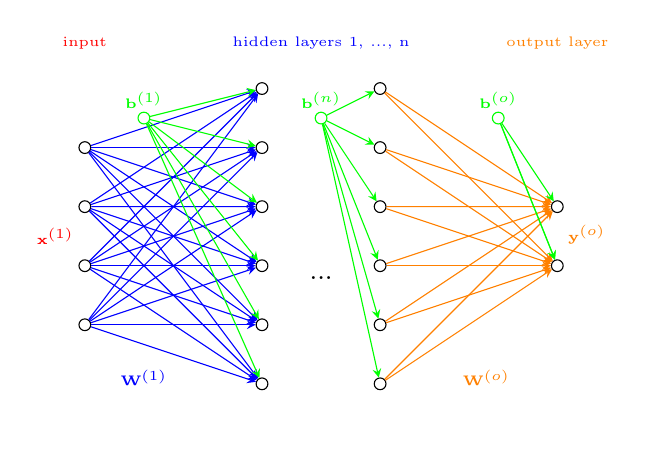
\begin{tikzpicture}[scale=1.5] 
\foreach \i in {0,...,3} \node[draw,circle,inner sep=1.5pt] (input\i) at (0,\the\numexpr0.5*\i+.5+0.75) {};
\foreach \i in {0,...,5} \node[draw,circle,inner sep=1.5pt] (hidden\i) at (1.5,\the\numexpr0.5*\i+0.75) {};
\foreach \i in {0,...,5} \node[draw,circle,inner sep=1.5pt] (hiddenl\i) at (2.5,\the\numexpr0.5*\i+0.75) {};
\foreach \i in {0,...,1} \node[draw,circle,inner sep=1.5pt] (output\i) at (4,\the\numexpr0.5*\i+1+.75) {};

% connectors input -> hidden
\foreach \i in {0,...,3}
\foreach \j in {0,...,5} \draw[-stealth,blue!100!white] (input\i) -- (hidden\j);

% connectors hidden -> output
\foreach \i in {0,...,5}
\foreach \j in {0,...,1} \draw[-stealth,orange!100!white] (hiddenl\i) -- (output\j);

% labels
\draw (input3) ++ (0.0,0.25+.5) node[red,above] {\tiny input};
\draw (output1) ++ (0.0,0.25+1.) node[orange,above] {\tiny output layer};
\draw (hidden5) ++ (0.5,0.25) node[blue,above] {\tiny hidden layers 1, ..., n};

%\draw (input0) ++ (-0.25,-0.20) node[red!100!white,above] {\tiny $x_1$};
\draw (input1) ++ (-0.25,.10) node[red!100!white,above] {\tiny $\mathbf{x}^{(1)}$};

%\draw (input1) ++ (-0.25,-0.20) node[red!100!white,above] {\tiny $x_0$};
%\draw (hiddenl5) ++ (0.0,0.25) node[blue,above] {\tiny hidden (n)};
\draw (output0) ++ (0.25,.10) node[orange,above] {\tiny $\mathbf{y}^{(o)}$};	
\draw (output0) ++ (0.25-2.25,-0.20) node[black,above] {...};	

% bias nodes
\node[color=green,draw,circle,inner sep=1.5pt] (bias1) at (0.5,5*0.5+0.5) {};
\draw (bias1) ++ (0.0,0.0) node[green,above] {\tiny $\textbf{b}^{\text{(1)}}$};

\node[color=green,draw,circle,inner sep=1.5pt] (bias3) at (0.5+1.5,5*0.5+0.5) {};
\draw (bias3) ++ (0.0,0.0) node[green,above] {\tiny $\textbf{b}^{\text{(n)}}$};

\node[color=green,draw,circle,inner sep=1.5pt] (bias2) at (2.25+1.25,5*0.5+0.5) {};
\draw (bias2) ++ (0.0,0.0) node[green,above] {\tiny $\textbf{b}^{\text{(o)}}$};

% bias connectors
\foreach \i in {0,...,5} \draw[-stealth,green!100!white] (bias1) -- (hidden\i);
\foreach \i in {0,...,5} \draw[-stealth,green!100!white] (bias3) -- (hiddenl\i);
\foreach \i in {0,...,1} \draw[-stealth,green!100!white] (bias2) -- (output\i);
\draw[-stealth,green!100!white] (bias2) -- (output0);

% weight labels
\draw (input0) ++ (0.5,-.6) node[blue!100!white,above] {\tiny $\textbf{W}^{\text{(1)}}$};
\draw (hiddenl0) ++ (.9,-0.1) node[orange!100!white,above] {\tiny $\textbf{W}^{\text{(o)}}$};

\node[draw,color=white] (dummy) at (0,0.5) {};
\end{tikzpicture}
	\caption[Single Hidden Layer Network]{Single Hidden Layer Network. The has two input, six hidden and one output unit. The sizes of the individual layers and the shape of the network is chosen to suit a target task.} 
	\label{hxcloseup}
\end{figure}
%\end{wrapfigure}
The training process of an \gls{ann} can be divided into a \emph{forward pass} where the output of all nodes is evaluated and a \emph{backward pass} which is responsible for the learning.

In the \textbf{forward pass}, the input $\mathbf{x}^{(l)}$ of a layer $l$ sums to a net input $\mathbf{a}^{(l)}$ of
\begin{align*}
\mathbf{a}^{(l)} = W^{(l)} \, \mathbf{x}^{(l)} + \mathbf{b}^{(l)} + \left(\text{noise}\right), 
\end{align*}
with the weight matrix $W^{(l)}$, the bias $\mathbf{b}^{(l)}$ and an optional noise term. The output $\mathbf{y}^{(l)}$ of the layer is then given by the activation function $\phi$, e.g. a sigmoid
\begin{equation*}
\mathbf{y}^{(l)} = \phi(\mathbf{a}^{(l)}) = \frac{1}{1 + e^{(-\beta \mathbf{a}^{(l)})}},
\end{equation*}
with a slope parameter $\beta$ of the sigmoid. Popular choices for the activation function are among others a \gls{relu}, a hyperbolic tangent ($\tanh$) or a sigmoid (see \cref{deeplearning_activation_functions} for comparison). For the context of this thesis, the sigmoid is the preferred option, which is mainly due to past usage of the function in internal projects.

However, it is important that the chosen function is non-linear. A linear activation function makes the layer structure redundant, as the composition of linear linear functions yields again a linear function and therefore all layers of a deep network could be merged into a single one.

Depending on the task, the bias as well as the optional noise term can be vital: the individual biases for instance allow the network to adjust the dynamic range of each neuron and the injection of artificial noise can significantly increase the training performance.

The same principle is then applied to all other layers to complete the forward pass, i.e. the result of the previous layer is the input for the current layer. The weight matrix $W^{\text{(l)}}$ connecting layer $l$ with $l-1$ has the appropriate shape to fit the number of input nodes $n^{\text{(l-1)}}_\text{nodes}$ and output nodes $n^{\text{(l)}}_\text{nodes}$.

\begin{figure}
	\begin{subfigure}[c]{0.5\textwidth}
		\centering
		\caption{}
		\inputpgf{figures}{deeplearning_activation_functions.pgf}
		\label{dltransfer}
	\end{subfigure}
	\begin{subfigure}[c]{0.5\textwidth}
		\centering
		\caption{}
		\inputpgf{figures}{deeplearning_activation_functions_derivative.pgf}	
		\label{dltransfergradient}
	\end{subfigure}
	\caption[Popular shapes for activation functions in deep learning.]{Popular shapes for activation functions in deep learning. \textbf{(\subref{dltransfer})}: Some of the most popular shapes for the activation function are a \gls{relu}, $\tanh$ or sigmoid. \textbf{(\subref{dltransfergradient})}: Training with a linear function would not work, because the gradient is a constant and does not discriminate between different inputs. A non-linear activation function is thus vital to the training. The \gls{relu} is, despite appearing to be a linear function at first glance, non-linear since it bends at $x=0$.}
	\label{deeplearning_activation_functions}
\end{figure}

In deep learning, gradient descent is probably the most popular algorithm to perform the \textbf{backward pass} on a network (\citealp{Goodfellow-et-al-2016}). A differentiable loss function $\loss(\mathbf{\mathbf{x}, y^*, \theta})$ for a given target $\textbf{y}^*$ is minimized by moving along the negative gradient of the loss with respect to the network's parameters $\mathbf{\theta}$. To avoid extensive computational costs, the gradient is estimated by a uniformly drawn subset of the full training data set, a \emph{minibatch}. In particular, if the size of the minibatch equals one, one speaks of \gls{sgd}.

Here, the loss function is chosen to be a binary cross-entropy loss
\begin{equation*}
\mathcal{L} = - \frac{1}{N} \sum_{i=1}^N \textbf{y}^* \log(\textbf{y}_i + (1-\textbf{y}^*) \log(1 - \textbf{y}_i), 
\end{equation*}
with a minibatch of size $N$ and the target $\textbf{y}^*$ being scaled between 0 and 1. In combination with a sigmoid-shaped activation function, this choice becomes convenient when computing the new set of parameters $\mathbf{\theta}'$ which is given by
\begin{equation}
\mathbf{\theta'} = \mathbf{\theta} - \eta \, \nabla_\theta\loss(\mathbf{\mathbf{x}, y^*, \mathbf{\theta}}),
\label{stochasticgradientdescent}
\end{equation}
with the learning rate $\eta$. As an example, the updates of the weight matrices of a single hidden layer network are computed in the next paragraphs using \gls{sgd}. 

First, the derivative of the cross entropy loss function in the output layer $l\equiv o$ is computed
\begin{equation*}
\frac{\partial\mathcal{L}}{\partial \mathbf{y}^{(o)}} = 
- \frac{\mathbf{y}^*}{\mathbf{y}^{(o)}} + 
\frac{1 - \mathbf{y}^*}{1 - \mathbf{y}^{(o)}},
\end{equation*}
The gradient of the loss can then be rewritten in terms of the error $\mathbf{e}^{(o)} = \mathbf{y}^* - \mathbf{y}^{(o)}$ by using the derivative of the activation function
\begin{align*}
\frac{\partial \mathbf{y}^{(o)}}{\partial \mathbf{a}^{(o)}} = \frac{\partial \gls{activation}(\mathbf{a}^{(o)})}{\partial \mathbf{a}^{(o)}} = \gls{activation} (1 - \gls{activation}),\\
\Rightarrow \quad \frac{\partial\mathcal{L}}{\partial \mathbf{a}^{(o)}} =
\frac{\partial\mathcal{L}}{\partial \mathbf{y}^{(o)}} 
\; \frac{\partial \mathbf{y}^{(o)}}{\partial \mathbf{a}^{(o)}} =
\mathbf{y}^* - \mathbf{y}^{(o)} = \mathbf{e}^{(o)}.
\end{align*}

According to \cref{stochasticgradientdescent}, the final update of the weight matrix is given by
\begin{equation}
\delta W^{(o)} = - \eta \frac{\partial \mathcal{L}}{\partial W^{(o)}} 
= - \eta \;
\frac{\partial\mathcal{L}}{\partial \mathbf{y}^{(o)}} \;
\frac{\partial \mathbf{a}^{(o)}}{\partial W^{(o)}}
= - \eta \, \left(\mathbf{e}^{(o)} \mathbf{x}^{(o),T}\right),
\label{backpropupdate}
\end{equation}

The computation for the hidden layer ($l\equiv h$) can be done in a similar fashion. Again, the gradient of the loss function is computed
\begin{equation*}
\frac{\partial\mathcal{L}}{\partial \mathbf{a}^{(h)}} = \mathbf{e}^{(h)} \;
\frac{\partial \mathbf{y}^{(h)} }{\partial \mathbf{a}^{(h)}},
\end{equation*}
and the error of the hidden layer $\mathbf{e}^{(h)}$ is propagated backwards as $\mathbf{e}^{(h)}=W^{(o),T}\mathbf{e}^{(o)}$ yielding a total update of
\begin{equation*}
\delta W^{\text{(h)}} = - \eta \;
\left(W^{\text{(o)}T} \mathbf{e}^{(o)}\right) \;
\frac{\partial \mathbf{y}^{(h)} }{\partial \mathbf{a}^{(h)}} \; \mathbf{x}^{(h), T}.
\end{equation*}

The backward propagation of the error is eponymous for the method's name \textit{backpropagation}. Despite the great performance for many deep learning tasks, the biological plausibility of propagating the error signal backward has been questioned ever since.

A simple but effective adjustment was suggested by \citealp{lillicrap2016random} which is also known as \textit{feedback alignment}. Instead of the transpose of the feed-forward weight matrix a fixed random matrix $B$ is chosen to propagate the error backwards. Compared to the backpropagation variant from \cref{backpropupdate} the update in the hidden layer changes to
\begin{equation*}
\delta W^{(h)} = - \eta \;
(B \mathbf{e}^{(o)}) \;
\frac{\partial \mathbf{y}^{(h)}}{\partial \mathbf{a}^{(h)}} \;
\mathbf{x}^{(h),T}.
\end{equation*}
The only constraints to $B$ are that $\mathbf{e}^{(o)T} W^{(o)} B \mathbf{e}^{(o)} > 0$ has to be fulfilled on average, meaning that geometrically, the new feedback signal $B \mathbf{e}^{(o)}$ for the hidden layer lies within $90^{\circ}$ of the one used by backprogation, $W^{\text{(o)}T} \mathbf{e}^{(o)}$.

%Q:Überleitung zu biologischem neuron hier?

\section{The Biological Neuron}

Biological neural networks have been a great inspiration for deep learning algorithms and \glspl{ann}. It is estimated that the human brain contains around $10^{11}$ neurons of different shape, size and functions (\citealp{numberofneurons}). By the use of \emph{synapses}, neurons create complex network structures throughout the brain. Usually a neuron has up to $10^4$ partners. The connections vary from dense clusters with nearby neurons to linking distant brain regions with each other.

The intercommunication is established by the use of short electrical pulses (spikes) and neurotransmitters. At most synapses, a small physical gap separates the neurons from each other, dividing them into a \emph{presynaptic} and \emph{postsynaptic} neuron. An electrical pulse of the presynaptic neuron releases various neurotransmitter to overcome this synaptic cleft. Once a transmitter has docked to a corresponding receptor on the other side, activated ion channels convert the chemical transmission back into an electrical signal. Depending on the type of neuro\-transmitters the excitation  can be excitatory or inhibitory. According to Dale's principle a presynaptic neuron releases always the same type of neurotransmitter. To that end, a neuron's output is either inhibitory or excitatory but not both. The input, on the other side, is not restricted to a single type of excitation, as various presynaptic partners can be connected.

On the postsynaptic side, the inputs of all presynaptic partners are then gathered by the \emph{dendrites} before they are forwarded to the \emph{soma} where the information is processed (c.f. \cref{biosynapse}). In particular, the soma integrates the currents induced by the input spikes, which can be tracked by measuring the course of the soma's membrane potential. The impact of each spike corresponds to a \gls{psp}. Once a certain threshold potential is reached, a mechanism gets triggered that initiates a fire response, the so-called action potential or spike. The neuron's membrane becomes hyperpolarized and decreases even below the resting potential as shown in \cref{actionpotential}. The neuron is in a so called \emph{refractory state} and due to the ongoing hyperpolarization it is hard but not impossible to fire. The action potentials are then relayed by the axon to its connected partners and the described course of communication starts over. 

\begin{figure}
	\begin{subfigure}{0.5\textwidth}
		\centering
		\caption{}
		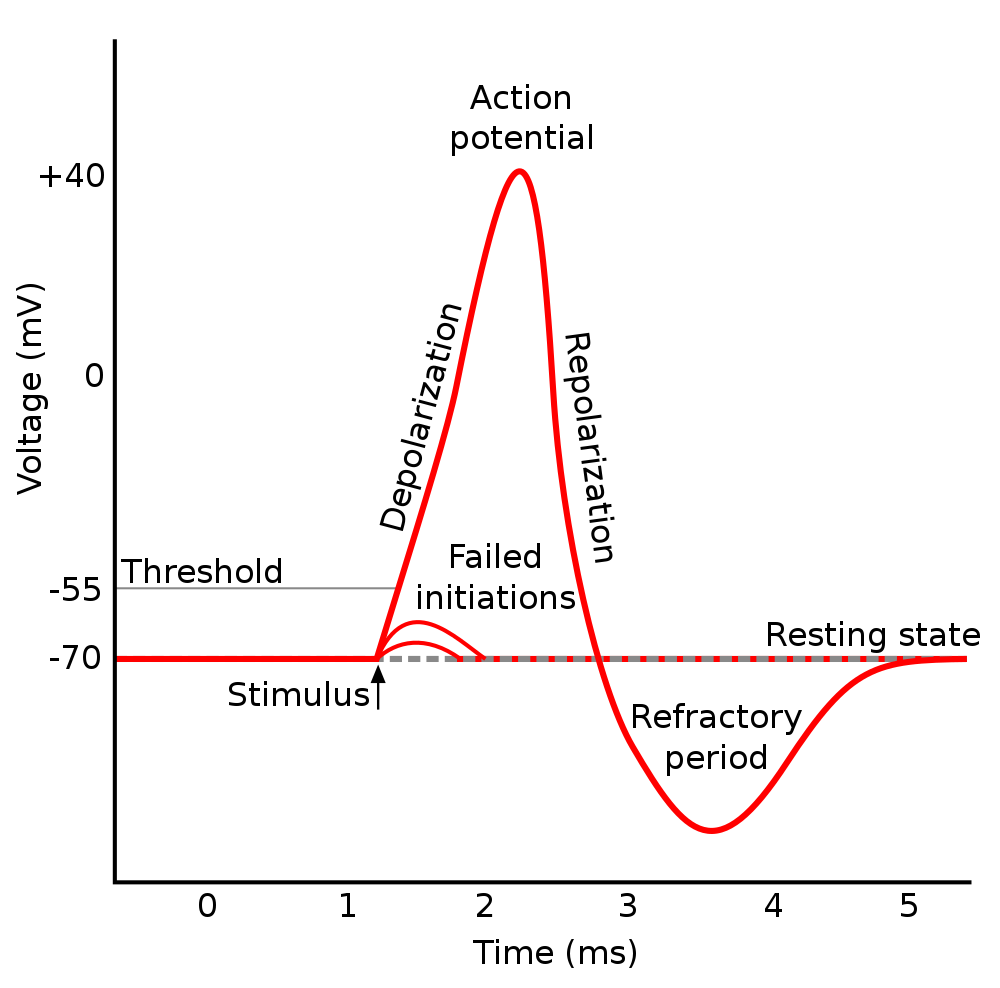
\includegraphics[width=0.8\linewidth, valign=t]{figures/action_potential.png}
		\label{actionpotential}
	\end{subfigure}
	\begin{subfigure}{0.5\textwidth}
		\centering
		\caption{}
		\vspace{0.5cm}
		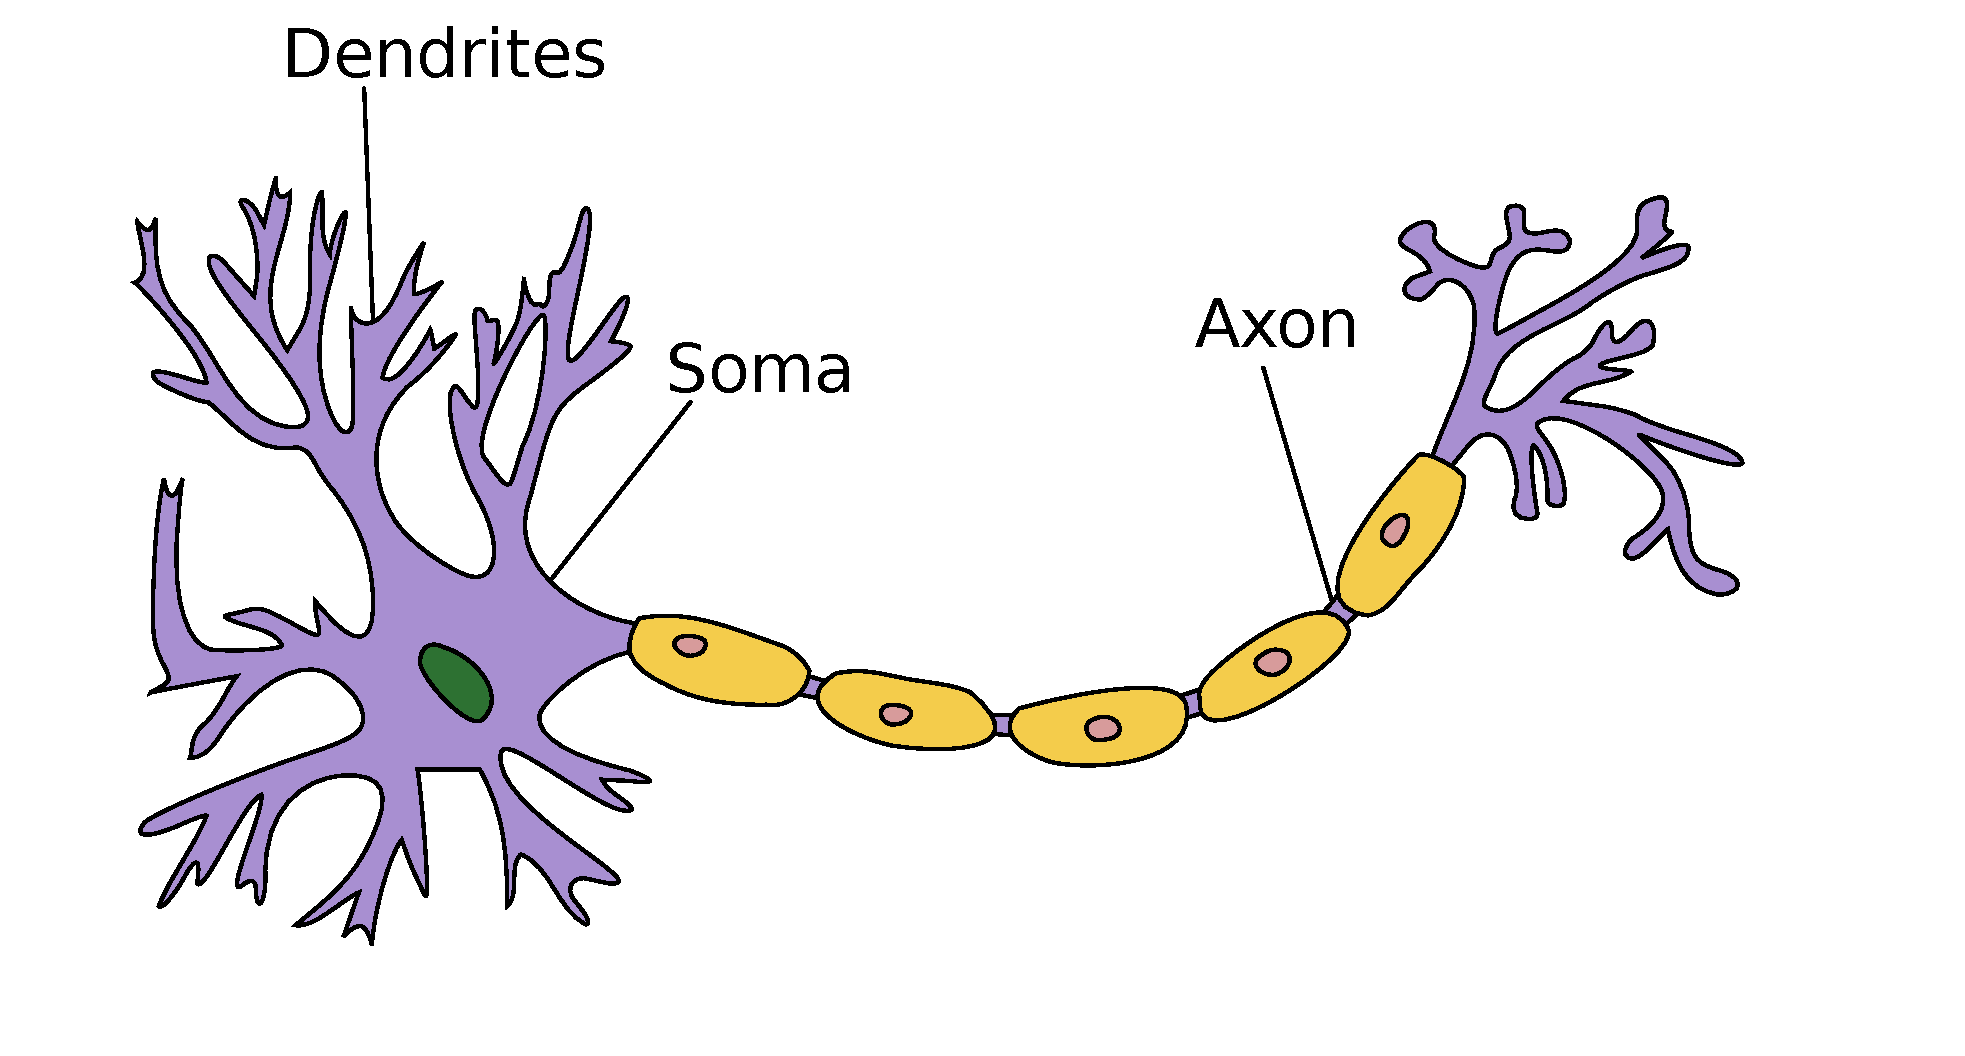
\includegraphics[width=\linewidth, valign=t]{figures/Neuron.pdf}
		\vspace{1.5cm}	
		\label{biosynapse}
	\end{subfigure}
	\caption[Schematics of an action potential and a biological neuron]{Schematics of a biological neuron and an action potential. \textbf{(\subref{actionpotential})} The response of neuron after exceeding the threshold is called action potential. After a phase of depolarization, the membrane repolarizes and enters the refractory state. Figure taken from \citealp{picture_actionpotential}. \textbf{(\subref{biosynapse})} Schematics of a biological neuron can be split into three main functional parts: the dendrites which are responsible to collect all inputs, the soma integrates the evoked \glspl{psp} and eventually triggers a fire response and the axon relays the fire responses to other neurons. Figure adapted from \citealp{picture_neuron}.}
	\label{biologicalneuron}
	
\end{figure}

Over time the unbalanced ion concentration in and outside the membrane is restored by the membranes permeability and additional ion pumps. In the equilibrated state, the membrane potential is then referred to as the \emph{resting potential}. The neurotransmitters are recycled as well. Otherwise, if their resources were depleted and heavily used synapses would be quickly silenced.

A wide-spread assumption in the field of neuroscience is that the exact shape of a spike doesn't carry any relevant information and therefore all spikes can be modeled by a stereotypical shape. The communication between neurons is then encoded in the frequency (\emph{rate coding}) or timing (\emph{time coding}) of exciting and inhibiting spikes. A more detailed description of neural coding schemes is presented in section \ref{neuralcoding}. However, recent research has already suggested that the small variations in the action potential contain vital information (\citealp{debanne2013mechanisms}).

The brain has a ability to continuously change the topology of its synaptic wiring, to create new synapses, to alter the chemical properties of the synaptic receptors or to simply strengthen and weaken the synaptic efficacy. With these plasticity mechanism the brain is able to learn and adapt as a reaction to stimulation or even damage.

One way of learning and forming memory is known as synaptic plasticity where the synaptic strength is changed over time. According to Hebb's theory ``neurons that fire together wire together" (\citealp{hebb1949organization}). An experimental proof of such activity-dependent plasticity was found by \citealp{bliss1973long}, where they discovered that a short but high frequency stimulation lead to a long lasting change in the synapse's efficacy. This is also referred to as \gls{ltp}. Reducing the stimulus to a low frequency, on the other hand, resulted in the opposite effect: \gls{ltd}. In combination they can carve out certain region in the brain which is related  to a stimulus and thereby create memory. 

A better understanding of \gls{ltp} and \gls{ltd} was provided by the introduction of \gls{stdp}. \gls{stdp} shows in principle that a presynaptic activity just before a postsynaptic response leads to an increase synaptic strength. If  presynaptic activity occurs right after a postsynaptic spike, the synapses is weakened (\citealp{poo98stdp}). 

%It is worth mentioning that synaptic plasticity between two neurons can also be induced by activity of an independent pathway. 

Developing biologically inspired and plausible learning algorithms is a dedicated goal in the field of modern neuroscience. In the next section a practicable neuron model is presented, which is the basis of the experimental part in this thesis.

\section{The \acrlong{lif} Model}

An early but successful description of the biological neuron dynamics was accomplished by the \glsfirst{lif} neuron, first described by \citealp{lapicque1907recherches}. Despite some strong simplifications, the main dynamics of the membrane potential are well described by the model and it thus has been a popular and portable choice for neuromorphic hardware implementations.

In biology, the observation of similar shaped individual action potentials lead to the assumption that the shape of a spike does not transport any information. The \gls{lif} model is based upon this theory and thus every spike can be replaced by a stereotypical shape.

Another observation in biology is that neurons vary much in their shape and size fulfilling different functions. The spatial component plays an important role for the dynamics of a neuron. For instance, the strategic positioning of certain excitatory or inhibitory inputs on the dendrites, either closer or farther away from the soma, give rise to non-linear behavior in the course of the membrane potential. However, extensive spatial dependencies are difficult and costly to implement in a model. Therefore, the \gls{lif} neuron neglects the topology of the neuron and is approximated as a point-like integrator. 

In the model, the incoming spike train $S_j(t)$ from various presynaptic partners $j$ is described by a series of spikes $s$ at times $t_j^{(s)}$
\begin{equation*}
S_j(t) = \sum_s \delta(t - t_j^{(s)}),
\end{equation*}
with the $\delta$-function denoted as $\delta$. 

Each spike of the input spike train evokes a \gls{psp}. The impact of the \glspl{psp} depends on the individual synaptic weights $w_j$. For simplicity, the excitatory or inhibitory nature of the synapses is encoded by a sign in the synaptic weight as well. Summing over all input sources yields a total synaptic input current that is seen by the postsynaptic neuron
\begin{equation}
\gls{isyn}(t) = \sum_j w_j \left(\epsilon \ast S_j(t)\right),
\label{synaptic_input}
\end{equation}
with an exponential kernel $\epsilon$ describing the shape of the \gls{psp}. Popular choices for the kernel are single or double-exponentials
\begin{align*}
\epsilon_\text{double}(t) 	&=\frac{1}{\mathcal{N}} \left(\epsilon_\text{rise} \ast \epsilon_\text{fall}\right)(t) \\
&=\frac{1}{\mathcal{N}}\exp \left(-\frac{t}{\tau_\text{rise}} \right)  \ast \exp \left(-\frac{t}{\tau_\text{fall}} \right), 
%\label{exponentialkernels)}
\end{align*}
with a rising and falling temporal constant $\tau_\text{rise}$ and $\tau_\text{fall}$ respectively. A constant $\mathcal{N}$ norms the kernel to unity. As the rising constant goes to zero $\tau_\text{rise} \rightarrow 0$ the double exponential turns into a single exponential kernel $\epsilon_\text{single} = \epsilon_\text{fall}$.

The membrane potential \gls{v_mem} changes with the continuous synaptic input causing an unbalanced ion concentration inside the membrane. Passive as well as active processes are permanently restoring the membrane potential back to its equilibrium state which is associated with the resting potential \gls{v_leak}. In the \gls{lif} model, the temporal scale of these restoring processes is defined by the membranes capacitance $C_\text{m}$ and the leakage conductance $g_\text{leak}$ yielding the membrane's time constant $\gls{tau_m} = \frac{C_\text{m}}{g_\text{leak}}$. The dynamics of membrane are then given by a single differential equation
\begin{align}
\label{lifeq}
C_{\text{m}} \frac{d\gls{v_mem}}{dt} &= -g_{\text{leak}} (\gls{v_mem} - \gls{v_leak}) + \gls{isyn}.
\end{align}

As for a biological neuron, the postsynaptic \gls{lif} neuron $i$ triggers a spike once a certain threshold \gls{thres} is crossed following the condition
\begin{equation*}
V_{\text{m}, i}\left(t_i^{(s)}\right) \ge \gls{thres} \Leftrightarrow \text{neuron \textit{i} fires at time } t_i^{(s)}.
\end{equation*}

Then the membrane is set to a reset potential \gls{v_reset} where it remains unchanged for a refractory period of \gls{refrac}
\begin{equation*}
V_{\text{m}, i}(t) = \gls{v_reset} \quad \forall t \in \left(t_i^{(s)}, t_i^{(s)} + \gls{refrac}\right].
\end{equation*}
Unlike for its biological counterpart, the modeled neuron cannot spike during the refractory period.

\begin{figure}
	\centering
	\scalebox{0.93}{%% Creator: Matplotlib, PGF backend
%%
%% To include the figure in your LaTeX document, write
%%   \input{<filename>.pgf}
%%
%% Make sure the required packages are loaded in your preamble
%%   \usepackage{pgf}
%%
%% Figures using additional raster images can only be included by \input if
%% they are in the same directory as the main LaTeX file. For loading figures
%% from other directories you can use the `import` package
%%   \usepackage{import}
%% and then include the figures with
%%   \import{<path to file>}{<filename>.pgf}
%%
%% Matplotlib used the following preamble
%%   \usepackage[utf8]{inputenc}
%%   \usepackage[T1]{fontenc}
%%   \usepackage{textcomp}
%%
\begingroup%
\makeatletter%
\begin{pgfpicture}%
\pgfpathrectangle{\pgfpointorigin}{\pgfqpoint{4.902605in}{2.799288in}}%
\pgfusepath{use as bounding box, clip}%
\begin{pgfscope}%
\pgfsetbuttcap%
\pgfsetmiterjoin%
\pgfsetlinewidth{0.000000pt}%
\definecolor{currentstroke}{rgb}{0.000000,0.000000,0.000000}%
\pgfsetstrokecolor{currentstroke}%
\pgfsetstrokeopacity{0.000000}%
\pgfsetdash{}{0pt}%
\pgfpathmoveto{\pgfqpoint{0.000000in}{0.000000in}}%
\pgfpathlineto{\pgfqpoint{4.902605in}{0.000000in}}%
\pgfpathlineto{\pgfqpoint{4.902605in}{2.799288in}}%
\pgfpathlineto{\pgfqpoint{0.000000in}{2.799288in}}%
\pgfpathclose%
\pgfusepath{}%
\end{pgfscope}%
\begin{pgfscope}%
\pgfsetbuttcap%
\pgfsetmiterjoin%
\pgfsetlinewidth{0.000000pt}%
\definecolor{currentstroke}{rgb}{0.000000,0.000000,0.000000}%
\pgfsetstrokecolor{currentstroke}%
\pgfsetstrokeopacity{0.000000}%
\pgfsetdash{}{0pt}%
\pgfpathmoveto{\pgfqpoint{0.585105in}{2.064876in}}%
\pgfpathlineto{\pgfqpoint{4.847605in}{2.064876in}}%
\pgfpathlineto{\pgfqpoint{4.847605in}{2.744288in}}%
\pgfpathlineto{\pgfqpoint{0.585105in}{2.744288in}}%
\pgfpathclose%
\pgfusepath{}%
\end{pgfscope}%
\begin{pgfscope}%
\pgfsetbuttcap%
\pgfsetroundjoin%
\definecolor{currentfill}{rgb}{0.200000,0.200000,0.200000}%
\pgfsetfillcolor{currentfill}%
\pgfsetlinewidth{0.803000pt}%
\definecolor{currentstroke}{rgb}{0.200000,0.200000,0.200000}%
\pgfsetstrokecolor{currentstroke}%
\pgfsetdash{}{0pt}%
\pgfsys@defobject{currentmarker}{\pgfqpoint{0.000000in}{-0.048611in}}{\pgfqpoint{0.000000in}{0.000000in}}{%
\pgfpathmoveto{\pgfqpoint{0.000000in}{0.000000in}}%
\pgfpathlineto{\pgfqpoint{0.000000in}{-0.048611in}}%
\pgfusepath{stroke,fill}%
}%
\begin{pgfscope}%
\pgfsys@transformshift{0.585105in}{2.064876in}%
\pgfsys@useobject{currentmarker}{}%
\end{pgfscope}%
\end{pgfscope}%
\begin{pgfscope}%
\pgfsetbuttcap%
\pgfsetroundjoin%
\definecolor{currentfill}{rgb}{0.200000,0.200000,0.200000}%
\pgfsetfillcolor{currentfill}%
\pgfsetlinewidth{0.803000pt}%
\definecolor{currentstroke}{rgb}{0.200000,0.200000,0.200000}%
\pgfsetstrokecolor{currentstroke}%
\pgfsetdash{}{0pt}%
\pgfsys@defobject{currentmarker}{\pgfqpoint{0.000000in}{-0.048611in}}{\pgfqpoint{0.000000in}{0.000000in}}{%
\pgfpathmoveto{\pgfqpoint{0.000000in}{0.000000in}}%
\pgfpathlineto{\pgfqpoint{0.000000in}{-0.048611in}}%
\pgfusepath{stroke,fill}%
}%
\begin{pgfscope}%
\pgfsys@transformshift{1.153438in}{2.064876in}%
\pgfsys@useobject{currentmarker}{}%
\end{pgfscope}%
\end{pgfscope}%
\begin{pgfscope}%
\pgfsetbuttcap%
\pgfsetroundjoin%
\definecolor{currentfill}{rgb}{0.200000,0.200000,0.200000}%
\pgfsetfillcolor{currentfill}%
\pgfsetlinewidth{0.803000pt}%
\definecolor{currentstroke}{rgb}{0.200000,0.200000,0.200000}%
\pgfsetstrokecolor{currentstroke}%
\pgfsetdash{}{0pt}%
\pgfsys@defobject{currentmarker}{\pgfqpoint{0.000000in}{-0.048611in}}{\pgfqpoint{0.000000in}{0.000000in}}{%
\pgfpathmoveto{\pgfqpoint{0.000000in}{0.000000in}}%
\pgfpathlineto{\pgfqpoint{0.000000in}{-0.048611in}}%
\pgfusepath{stroke,fill}%
}%
\begin{pgfscope}%
\pgfsys@transformshift{1.721772in}{2.064876in}%
\pgfsys@useobject{currentmarker}{}%
\end{pgfscope}%
\end{pgfscope}%
\begin{pgfscope}%
\pgfsetbuttcap%
\pgfsetroundjoin%
\definecolor{currentfill}{rgb}{0.200000,0.200000,0.200000}%
\pgfsetfillcolor{currentfill}%
\pgfsetlinewidth{0.803000pt}%
\definecolor{currentstroke}{rgb}{0.200000,0.200000,0.200000}%
\pgfsetstrokecolor{currentstroke}%
\pgfsetdash{}{0pt}%
\pgfsys@defobject{currentmarker}{\pgfqpoint{0.000000in}{-0.048611in}}{\pgfqpoint{0.000000in}{0.000000in}}{%
\pgfpathmoveto{\pgfqpoint{0.000000in}{0.000000in}}%
\pgfpathlineto{\pgfqpoint{0.000000in}{-0.048611in}}%
\pgfusepath{stroke,fill}%
}%
\begin{pgfscope}%
\pgfsys@transformshift{2.290105in}{2.064876in}%
\pgfsys@useobject{currentmarker}{}%
\end{pgfscope}%
\end{pgfscope}%
\begin{pgfscope}%
\pgfsetbuttcap%
\pgfsetroundjoin%
\definecolor{currentfill}{rgb}{0.200000,0.200000,0.200000}%
\pgfsetfillcolor{currentfill}%
\pgfsetlinewidth{0.803000pt}%
\definecolor{currentstroke}{rgb}{0.200000,0.200000,0.200000}%
\pgfsetstrokecolor{currentstroke}%
\pgfsetdash{}{0pt}%
\pgfsys@defobject{currentmarker}{\pgfqpoint{0.000000in}{-0.048611in}}{\pgfqpoint{0.000000in}{0.000000in}}{%
\pgfpathmoveto{\pgfqpoint{0.000000in}{0.000000in}}%
\pgfpathlineto{\pgfqpoint{0.000000in}{-0.048611in}}%
\pgfusepath{stroke,fill}%
}%
\begin{pgfscope}%
\pgfsys@transformshift{2.858438in}{2.064876in}%
\pgfsys@useobject{currentmarker}{}%
\end{pgfscope}%
\end{pgfscope}%
\begin{pgfscope}%
\pgfsetbuttcap%
\pgfsetroundjoin%
\definecolor{currentfill}{rgb}{0.200000,0.200000,0.200000}%
\pgfsetfillcolor{currentfill}%
\pgfsetlinewidth{0.803000pt}%
\definecolor{currentstroke}{rgb}{0.200000,0.200000,0.200000}%
\pgfsetstrokecolor{currentstroke}%
\pgfsetdash{}{0pt}%
\pgfsys@defobject{currentmarker}{\pgfqpoint{0.000000in}{-0.048611in}}{\pgfqpoint{0.000000in}{0.000000in}}{%
\pgfpathmoveto{\pgfqpoint{0.000000in}{0.000000in}}%
\pgfpathlineto{\pgfqpoint{0.000000in}{-0.048611in}}%
\pgfusepath{stroke,fill}%
}%
\begin{pgfscope}%
\pgfsys@transformshift{3.426772in}{2.064876in}%
\pgfsys@useobject{currentmarker}{}%
\end{pgfscope}%
\end{pgfscope}%
\begin{pgfscope}%
\pgfsetbuttcap%
\pgfsetroundjoin%
\definecolor{currentfill}{rgb}{0.200000,0.200000,0.200000}%
\pgfsetfillcolor{currentfill}%
\pgfsetlinewidth{0.803000pt}%
\definecolor{currentstroke}{rgb}{0.200000,0.200000,0.200000}%
\pgfsetstrokecolor{currentstroke}%
\pgfsetdash{}{0pt}%
\pgfsys@defobject{currentmarker}{\pgfqpoint{0.000000in}{-0.048611in}}{\pgfqpoint{0.000000in}{0.000000in}}{%
\pgfpathmoveto{\pgfqpoint{0.000000in}{0.000000in}}%
\pgfpathlineto{\pgfqpoint{0.000000in}{-0.048611in}}%
\pgfusepath{stroke,fill}%
}%
\begin{pgfscope}%
\pgfsys@transformshift{3.995105in}{2.064876in}%
\pgfsys@useobject{currentmarker}{}%
\end{pgfscope}%
\end{pgfscope}%
\begin{pgfscope}%
\pgfsetbuttcap%
\pgfsetroundjoin%
\definecolor{currentfill}{rgb}{0.200000,0.200000,0.200000}%
\pgfsetfillcolor{currentfill}%
\pgfsetlinewidth{0.803000pt}%
\definecolor{currentstroke}{rgb}{0.200000,0.200000,0.200000}%
\pgfsetstrokecolor{currentstroke}%
\pgfsetdash{}{0pt}%
\pgfsys@defobject{currentmarker}{\pgfqpoint{0.000000in}{-0.048611in}}{\pgfqpoint{0.000000in}{0.000000in}}{%
\pgfpathmoveto{\pgfqpoint{0.000000in}{0.000000in}}%
\pgfpathlineto{\pgfqpoint{0.000000in}{-0.048611in}}%
\pgfusepath{stroke,fill}%
}%
\begin{pgfscope}%
\pgfsys@transformshift{4.563438in}{2.064876in}%
\pgfsys@useobject{currentmarker}{}%
\end{pgfscope}%
\end{pgfscope}%
\begin{pgfscope}%
\pgfpathrectangle{\pgfqpoint{0.585105in}{2.064876in}}{\pgfqpoint{4.262500in}{0.679412in}} %
\pgfusepath{clip}%
\pgfsetrectcap%
\pgfsetroundjoin%
\pgfsetlinewidth{0.803000pt}%
\definecolor{currentstroke}{rgb}{0.690196,0.690196,0.690196}%
\pgfsetstrokecolor{currentstroke}%
\pgfsetstrokeopacity{0.300000}%
\pgfsetdash{}{0pt}%
\pgfpathmoveto{\pgfqpoint{0.585105in}{2.214661in}}%
\pgfpathlineto{\pgfqpoint{4.847605in}{2.214661in}}%
\pgfusepath{stroke}%
\end{pgfscope}%
\begin{pgfscope}%
\pgfsetbuttcap%
\pgfsetroundjoin%
\definecolor{currentfill}{rgb}{0.200000,0.200000,0.200000}%
\pgfsetfillcolor{currentfill}%
\pgfsetlinewidth{0.803000pt}%
\definecolor{currentstroke}{rgb}{0.200000,0.200000,0.200000}%
\pgfsetstrokecolor{currentstroke}%
\pgfsetdash{}{0pt}%
\pgfsys@defobject{currentmarker}{\pgfqpoint{-0.048611in}{0.000000in}}{\pgfqpoint{0.000000in}{0.000000in}}{%
\pgfpathmoveto{\pgfqpoint{0.000000in}{0.000000in}}%
\pgfpathlineto{\pgfqpoint{-0.048611in}{0.000000in}}%
\pgfusepath{stroke,fill}%
}%
\begin{pgfscope}%
\pgfsys@transformshift{0.585105in}{2.214661in}%
\pgfsys@useobject{currentmarker}{}%
\end{pgfscope}%
\end{pgfscope}%
\begin{pgfscope}%
\definecolor{textcolor}{rgb}{0.200000,0.200000,0.200000}%
\pgfsetstrokecolor{textcolor}%
\pgfsetfillcolor{textcolor}%
\pgftext[x=0.240968in,y=2.166833in,left,base]{\color{textcolor}\rmfamily\fontsize{10.000000}{12.000000}\selectfont \(\displaystyle -60\)}%
\end{pgfscope}%
\begin{pgfscope}%
\pgfpathrectangle{\pgfqpoint{0.585105in}{2.064876in}}{\pgfqpoint{4.262500in}{0.679412in}} %
\pgfusepath{clip}%
\pgfsetrectcap%
\pgfsetroundjoin%
\pgfsetlinewidth{0.803000pt}%
\definecolor{currentstroke}{rgb}{0.690196,0.690196,0.690196}%
\pgfsetstrokecolor{currentstroke}%
\pgfsetstrokeopacity{0.300000}%
\pgfsetdash{}{0pt}%
\pgfpathmoveto{\pgfqpoint{0.585105in}{2.690272in}}%
\pgfpathlineto{\pgfqpoint{4.847605in}{2.690272in}}%
\pgfusepath{stroke}%
\end{pgfscope}%
\begin{pgfscope}%
\pgfsetbuttcap%
\pgfsetroundjoin%
\definecolor{currentfill}{rgb}{0.200000,0.200000,0.200000}%
\pgfsetfillcolor{currentfill}%
\pgfsetlinewidth{0.803000pt}%
\definecolor{currentstroke}{rgb}{0.200000,0.200000,0.200000}%
\pgfsetstrokecolor{currentstroke}%
\pgfsetdash{}{0pt}%
\pgfsys@defobject{currentmarker}{\pgfqpoint{-0.048611in}{0.000000in}}{\pgfqpoint{0.000000in}{0.000000in}}{%
\pgfpathmoveto{\pgfqpoint{0.000000in}{0.000000in}}%
\pgfpathlineto{\pgfqpoint{-0.048611in}{0.000000in}}%
\pgfusepath{stroke,fill}%
}%
\begin{pgfscope}%
\pgfsys@transformshift{0.585105in}{2.690272in}%
\pgfsys@useobject{currentmarker}{}%
\end{pgfscope}%
\end{pgfscope}%
\begin{pgfscope}%
\definecolor{textcolor}{rgb}{0.200000,0.200000,0.200000}%
\pgfsetstrokecolor{textcolor}%
\pgfsetfillcolor{textcolor}%
\pgftext[x=0.240968in,y=2.642444in,left,base]{\color{textcolor}\rmfamily\fontsize{10.000000}{12.000000}\selectfont \(\displaystyle -40\)}%
\end{pgfscope}%
\begin{pgfscope}%
\pgftext[x=0.185413in,y=2.404582in,,bottom,rotate=90.000000]{\rmfamily\fontsize{10.000000}{12.000000}\selectfont \(\displaystyle V^\mathrm{LIF}_\mathrm{m}\) [mV]}%
\end{pgfscope}%
\begin{pgfscope}%
\pgfpathrectangle{\pgfqpoint{0.585105in}{2.064876in}}{\pgfqpoint{4.262500in}{0.679412in}} %
\pgfusepath{clip}%
\pgfsetrectcap%
\pgfsetroundjoin%
\pgfsetlinewidth{0.501875pt}%
\definecolor{currentstroke}{rgb}{0.400000,0.400000,0.400000}%
\pgfsetstrokecolor{currentstroke}%
\pgfsetdash{}{0pt}%
\pgfpathmoveto{\pgfqpoint{0.585105in}{2.214661in}}%
\pgfpathlineto{\pgfqpoint{1.153438in}{2.214661in}}%
\pgfpathlineto{\pgfqpoint{1.165373in}{2.248444in}}%
\pgfpathlineto{\pgfqpoint{1.177308in}{2.275828in}}%
\pgfpathlineto{\pgfqpoint{1.189812in}{2.298970in}}%
\pgfpathlineto{\pgfqpoint{1.202315in}{2.317542in}}%
\pgfpathlineto{\pgfqpoint{1.215387in}{2.333049in}}%
\pgfpathlineto{\pgfqpoint{1.229027in}{2.345844in}}%
\pgfpathlineto{\pgfqpoint{1.243803in}{2.356644in}}%
\pgfpathlineto{\pgfqpoint{1.259717in}{2.365526in}}%
\pgfpathlineto{\pgfqpoint{1.277903in}{2.373054in}}%
\pgfpathlineto{\pgfqpoint{1.298932in}{2.379227in}}%
\pgfpathlineto{\pgfqpoint{1.323938in}{2.384135in}}%
\pgfpathlineto{\pgfqpoint{1.355197in}{2.387892in}}%
\pgfpathlineto{\pgfqpoint{1.397253in}{2.390571in}}%
\pgfpathlineto{\pgfqpoint{1.462043in}{2.392233in}}%
\pgfpathlineto{\pgfqpoint{1.594465in}{2.392939in}}%
\pgfpathlineto{\pgfqpoint{1.727455in}{2.393008in}}%
\pgfpathlineto{\pgfqpoint{1.739390in}{2.359226in}}%
\pgfpathlineto{\pgfqpoint{1.751325in}{2.331843in}}%
\pgfpathlineto{\pgfqpoint{1.763828in}{2.308702in}}%
\pgfpathlineto{\pgfqpoint{1.776332in}{2.290131in}}%
\pgfpathlineto{\pgfqpoint{1.789403in}{2.274624in}}%
\pgfpathlineto{\pgfqpoint{1.803043in}{2.261830in}}%
\pgfpathlineto{\pgfqpoint{1.817820in}{2.251031in}}%
\pgfpathlineto{\pgfqpoint{1.833733in}{2.242149in}}%
\pgfpathlineto{\pgfqpoint{1.851920in}{2.234621in}}%
\pgfpathlineto{\pgfqpoint{1.872948in}{2.228448in}}%
\pgfpathlineto{\pgfqpoint{1.897955in}{2.223540in}}%
\pgfpathlineto{\pgfqpoint{1.929213in}{2.219784in}}%
\pgfpathlineto{\pgfqpoint{1.971270in}{2.217105in}}%
\pgfpathlineto{\pgfqpoint{2.036060in}{2.215443in}}%
\pgfpathlineto{\pgfqpoint{2.168482in}{2.214737in}}%
\pgfpathlineto{\pgfqpoint{2.869805in}{2.214661in}}%
\pgfpathlineto{\pgfqpoint{2.881740in}{2.263309in}}%
\pgfpathlineto{\pgfqpoint{2.893675in}{2.302742in}}%
\pgfpathlineto{\pgfqpoint{2.905610in}{2.334705in}}%
\pgfpathlineto{\pgfqpoint{2.917545in}{2.360615in}}%
\pgfpathlineto{\pgfqpoint{2.930048in}{2.382511in}}%
\pgfpathlineto{\pgfqpoint{2.942552in}{2.400083in}}%
\pgfpathlineto{\pgfqpoint{2.955623in}{2.414754in}}%
\pgfpathlineto{\pgfqpoint{2.969832in}{2.427305in}}%
\pgfpathlineto{\pgfqpoint{2.984608in}{2.437421in}}%
\pgfpathlineto{\pgfqpoint{3.001090in}{2.445997in}}%
\pgfpathlineto{\pgfqpoint{3.017572in}{2.452415in}}%
\pgfpathlineto{\pgfqpoint{3.018708in}{2.095759in}}%
\pgfpathlineto{\pgfqpoint{3.074405in}{2.095759in}}%
\pgfpathlineto{\pgfqpoint{3.086340in}{2.166928in}}%
\pgfpathlineto{\pgfqpoint{3.098275in}{2.224617in}}%
\pgfpathlineto{\pgfqpoint{3.110210in}{2.271379in}}%
\pgfpathlineto{\pgfqpoint{3.122145in}{2.309283in}}%
\pgfpathlineto{\pgfqpoint{3.134080in}{2.340008in}}%
\pgfpathlineto{\pgfqpoint{3.146015in}{2.364913in}}%
\pgfpathlineto{\pgfqpoint{3.158518in}{2.385960in}}%
\pgfpathlineto{\pgfqpoint{3.171590in}{2.403534in}}%
\pgfpathlineto{\pgfqpoint{3.184662in}{2.417497in}}%
\pgfpathlineto{\pgfqpoint{3.198870in}{2.429440in}}%
\pgfpathlineto{\pgfqpoint{3.214215in}{2.439390in}}%
\pgfpathlineto{\pgfqpoint{3.231265in}{2.447710in}}%
\pgfpathlineto{\pgfqpoint{3.243768in}{2.452406in}}%
\pgfpathlineto{\pgfqpoint{3.244905in}{2.095759in}}%
\pgfpathlineto{\pgfqpoint{3.300602in}{2.095759in}}%
\pgfpathlineto{\pgfqpoint{3.312537in}{2.166928in}}%
\pgfpathlineto{\pgfqpoint{3.324472in}{2.224617in}}%
\pgfpathlineto{\pgfqpoint{3.336407in}{2.271379in}}%
\pgfpathlineto{\pgfqpoint{3.348342in}{2.309283in}}%
\pgfpathlineto{\pgfqpoint{3.360277in}{2.340008in}}%
\pgfpathlineto{\pgfqpoint{3.372212in}{2.364913in}}%
\pgfpathlineto{\pgfqpoint{3.384715in}{2.385960in}}%
\pgfpathlineto{\pgfqpoint{3.397787in}{2.403534in}}%
\pgfpathlineto{\pgfqpoint{3.410858in}{2.417497in}}%
\pgfpathlineto{\pgfqpoint{3.425067in}{2.429440in}}%
\pgfpathlineto{\pgfqpoint{3.440412in}{2.439390in}}%
\pgfpathlineto{\pgfqpoint{3.457462in}{2.447710in}}%
\pgfpathlineto{\pgfqpoint{3.469965in}{2.452406in}}%
\pgfpathlineto{\pgfqpoint{3.471102in}{2.095759in}}%
\pgfpathlineto{\pgfqpoint{3.526798in}{2.095759in}}%
\pgfpathlineto{\pgfqpoint{3.538733in}{2.166928in}}%
\pgfpathlineto{\pgfqpoint{3.550668in}{2.224617in}}%
\pgfpathlineto{\pgfqpoint{3.562603in}{2.271379in}}%
\pgfpathlineto{\pgfqpoint{3.574538in}{2.309283in}}%
\pgfpathlineto{\pgfqpoint{3.586473in}{2.340008in}}%
\pgfpathlineto{\pgfqpoint{3.598408in}{2.364913in}}%
\pgfpathlineto{\pgfqpoint{3.610912in}{2.385960in}}%
\pgfpathlineto{\pgfqpoint{3.623983in}{2.403534in}}%
\pgfpathlineto{\pgfqpoint{3.637055in}{2.417497in}}%
\pgfpathlineto{\pgfqpoint{3.651263in}{2.429440in}}%
\pgfpathlineto{\pgfqpoint{3.666608in}{2.439390in}}%
\pgfpathlineto{\pgfqpoint{3.683658in}{2.447710in}}%
\pgfpathlineto{\pgfqpoint{3.696162in}{2.452406in}}%
\pgfpathlineto{\pgfqpoint{3.697298in}{2.095759in}}%
\pgfpathlineto{\pgfqpoint{3.752995in}{2.095759in}}%
\pgfpathlineto{\pgfqpoint{3.764930in}{2.166928in}}%
\pgfpathlineto{\pgfqpoint{3.776865in}{2.224617in}}%
\pgfpathlineto{\pgfqpoint{3.788800in}{2.271379in}}%
\pgfpathlineto{\pgfqpoint{3.800735in}{2.309283in}}%
\pgfpathlineto{\pgfqpoint{3.812670in}{2.340008in}}%
\pgfpathlineto{\pgfqpoint{3.824605in}{2.364913in}}%
\pgfpathlineto{\pgfqpoint{3.837108in}{2.385960in}}%
\pgfpathlineto{\pgfqpoint{3.850180in}{2.403534in}}%
\pgfpathlineto{\pgfqpoint{3.863252in}{2.417497in}}%
\pgfpathlineto{\pgfqpoint{3.877460in}{2.429440in}}%
\pgfpathlineto{\pgfqpoint{3.892805in}{2.439390in}}%
\pgfpathlineto{\pgfqpoint{3.909855in}{2.447710in}}%
\pgfpathlineto{\pgfqpoint{3.922358in}{2.452406in}}%
\pgfpathlineto{\pgfqpoint{3.923495in}{2.095759in}}%
\pgfpathlineto{\pgfqpoint{3.979192in}{2.095759in}}%
\pgfpathlineto{\pgfqpoint{3.991127in}{2.166928in}}%
\pgfpathlineto{\pgfqpoint{4.003062in}{2.224617in}}%
\pgfpathlineto{\pgfqpoint{4.012155in}{2.261119in}}%
\pgfpathlineto{\pgfqpoint{4.026932in}{2.250482in}}%
\pgfpathlineto{\pgfqpoint{4.042845in}{2.241734in}}%
\pgfpathlineto{\pgfqpoint{4.061032in}{2.234320in}}%
\pgfpathlineto{\pgfqpoint{4.082060in}{2.228240in}}%
\pgfpathlineto{\pgfqpoint{4.107067in}{2.223407in}}%
\pgfpathlineto{\pgfqpoint{4.138893in}{2.219657in}}%
\pgfpathlineto{\pgfqpoint{4.181518in}{2.217021in}}%
\pgfpathlineto{\pgfqpoint{4.247445in}{2.215401in}}%
\pgfpathlineto{\pgfqpoint{4.384982in}{2.214727in}}%
\pgfpathlineto{\pgfqpoint{4.848173in}{2.214661in}}%
\pgfpathlineto{\pgfqpoint{4.848173in}{2.214661in}}%
\pgfusepath{stroke}%
\end{pgfscope}%
\begin{pgfscope}%
\pgfsetrectcap%
\pgfsetmiterjoin%
\pgfsetlinewidth{0.803000pt}%
\definecolor{currentstroke}{rgb}{0.200000,0.200000,0.200000}%
\pgfsetstrokecolor{currentstroke}%
\pgfsetdash{}{0pt}%
\pgfpathmoveto{\pgfqpoint{0.585105in}{2.064876in}}%
\pgfpathlineto{\pgfqpoint{0.585105in}{2.744288in}}%
\pgfusepath{stroke}%
\end{pgfscope}%
\begin{pgfscope}%
\pgfsetrectcap%
\pgfsetmiterjoin%
\pgfsetlinewidth{0.803000pt}%
\definecolor{currentstroke}{rgb}{0.200000,0.200000,0.200000}%
\pgfsetstrokecolor{currentstroke}%
\pgfsetdash{}{0pt}%
\pgfpathmoveto{\pgfqpoint{0.585105in}{2.064876in}}%
\pgfpathlineto{\pgfqpoint{4.847605in}{2.064876in}}%
\pgfusepath{stroke}%
\end{pgfscope}%
\begin{pgfscope}%
\definecolor{textcolor}{rgb}{0.200000,0.200000,0.200000}%
\pgfsetstrokecolor{textcolor}%
\pgfsetfillcolor{textcolor}%
\pgftext[x=0.670355in,y=2.642376in,left,top]{\color{textcolor}\rmfamily\fontsize{10.000000}{12.000000}\selectfont (a)}%
\end{pgfscope}%
\begin{pgfscope}%
\pgfsetbuttcap%
\pgfsetmiterjoin%
\pgfsetlinewidth{0.000000pt}%
\definecolor{currentstroke}{rgb}{0.000000,0.000000,0.000000}%
\pgfsetstrokecolor{currentstroke}%
\pgfsetstrokeopacity{0.000000}%
\pgfsetdash{}{0pt}%
\pgfpathmoveto{\pgfqpoint{0.585105in}{1.249582in}}%
\pgfpathlineto{\pgfqpoint{4.847605in}{1.249582in}}%
\pgfpathlineto{\pgfqpoint{4.847605in}{1.928994in}}%
\pgfpathlineto{\pgfqpoint{0.585105in}{1.928994in}}%
\pgfpathclose%
\pgfusepath{}%
\end{pgfscope}%
\begin{pgfscope}%
\pgfsetbuttcap%
\pgfsetroundjoin%
\definecolor{currentfill}{rgb}{0.200000,0.200000,0.200000}%
\pgfsetfillcolor{currentfill}%
\pgfsetlinewidth{0.803000pt}%
\definecolor{currentstroke}{rgb}{0.200000,0.200000,0.200000}%
\pgfsetstrokecolor{currentstroke}%
\pgfsetdash{}{0pt}%
\pgfsys@defobject{currentmarker}{\pgfqpoint{0.000000in}{-0.048611in}}{\pgfqpoint{0.000000in}{0.000000in}}{%
\pgfpathmoveto{\pgfqpoint{0.000000in}{0.000000in}}%
\pgfpathlineto{\pgfqpoint{0.000000in}{-0.048611in}}%
\pgfusepath{stroke,fill}%
}%
\begin{pgfscope}%
\pgfsys@transformshift{0.585105in}{1.249582in}%
\pgfsys@useobject{currentmarker}{}%
\end{pgfscope}%
\end{pgfscope}%
\begin{pgfscope}%
\pgfsetbuttcap%
\pgfsetroundjoin%
\definecolor{currentfill}{rgb}{0.200000,0.200000,0.200000}%
\pgfsetfillcolor{currentfill}%
\pgfsetlinewidth{0.803000pt}%
\definecolor{currentstroke}{rgb}{0.200000,0.200000,0.200000}%
\pgfsetstrokecolor{currentstroke}%
\pgfsetdash{}{0pt}%
\pgfsys@defobject{currentmarker}{\pgfqpoint{0.000000in}{-0.048611in}}{\pgfqpoint{0.000000in}{0.000000in}}{%
\pgfpathmoveto{\pgfqpoint{0.000000in}{0.000000in}}%
\pgfpathlineto{\pgfqpoint{0.000000in}{-0.048611in}}%
\pgfusepath{stroke,fill}%
}%
\begin{pgfscope}%
\pgfsys@transformshift{1.153438in}{1.249582in}%
\pgfsys@useobject{currentmarker}{}%
\end{pgfscope}%
\end{pgfscope}%
\begin{pgfscope}%
\pgfsetbuttcap%
\pgfsetroundjoin%
\definecolor{currentfill}{rgb}{0.200000,0.200000,0.200000}%
\pgfsetfillcolor{currentfill}%
\pgfsetlinewidth{0.803000pt}%
\definecolor{currentstroke}{rgb}{0.200000,0.200000,0.200000}%
\pgfsetstrokecolor{currentstroke}%
\pgfsetdash{}{0pt}%
\pgfsys@defobject{currentmarker}{\pgfqpoint{0.000000in}{-0.048611in}}{\pgfqpoint{0.000000in}{0.000000in}}{%
\pgfpathmoveto{\pgfqpoint{0.000000in}{0.000000in}}%
\pgfpathlineto{\pgfqpoint{0.000000in}{-0.048611in}}%
\pgfusepath{stroke,fill}%
}%
\begin{pgfscope}%
\pgfsys@transformshift{1.721772in}{1.249582in}%
\pgfsys@useobject{currentmarker}{}%
\end{pgfscope}%
\end{pgfscope}%
\begin{pgfscope}%
\pgfsetbuttcap%
\pgfsetroundjoin%
\definecolor{currentfill}{rgb}{0.200000,0.200000,0.200000}%
\pgfsetfillcolor{currentfill}%
\pgfsetlinewidth{0.803000pt}%
\definecolor{currentstroke}{rgb}{0.200000,0.200000,0.200000}%
\pgfsetstrokecolor{currentstroke}%
\pgfsetdash{}{0pt}%
\pgfsys@defobject{currentmarker}{\pgfqpoint{0.000000in}{-0.048611in}}{\pgfqpoint{0.000000in}{0.000000in}}{%
\pgfpathmoveto{\pgfqpoint{0.000000in}{0.000000in}}%
\pgfpathlineto{\pgfqpoint{0.000000in}{-0.048611in}}%
\pgfusepath{stroke,fill}%
}%
\begin{pgfscope}%
\pgfsys@transformshift{2.290105in}{1.249582in}%
\pgfsys@useobject{currentmarker}{}%
\end{pgfscope}%
\end{pgfscope}%
\begin{pgfscope}%
\pgfsetbuttcap%
\pgfsetroundjoin%
\definecolor{currentfill}{rgb}{0.200000,0.200000,0.200000}%
\pgfsetfillcolor{currentfill}%
\pgfsetlinewidth{0.803000pt}%
\definecolor{currentstroke}{rgb}{0.200000,0.200000,0.200000}%
\pgfsetstrokecolor{currentstroke}%
\pgfsetdash{}{0pt}%
\pgfsys@defobject{currentmarker}{\pgfqpoint{0.000000in}{-0.048611in}}{\pgfqpoint{0.000000in}{0.000000in}}{%
\pgfpathmoveto{\pgfqpoint{0.000000in}{0.000000in}}%
\pgfpathlineto{\pgfqpoint{0.000000in}{-0.048611in}}%
\pgfusepath{stroke,fill}%
}%
\begin{pgfscope}%
\pgfsys@transformshift{2.858438in}{1.249582in}%
\pgfsys@useobject{currentmarker}{}%
\end{pgfscope}%
\end{pgfscope}%
\begin{pgfscope}%
\pgfsetbuttcap%
\pgfsetroundjoin%
\definecolor{currentfill}{rgb}{0.200000,0.200000,0.200000}%
\pgfsetfillcolor{currentfill}%
\pgfsetlinewidth{0.803000pt}%
\definecolor{currentstroke}{rgb}{0.200000,0.200000,0.200000}%
\pgfsetstrokecolor{currentstroke}%
\pgfsetdash{}{0pt}%
\pgfsys@defobject{currentmarker}{\pgfqpoint{0.000000in}{-0.048611in}}{\pgfqpoint{0.000000in}{0.000000in}}{%
\pgfpathmoveto{\pgfqpoint{0.000000in}{0.000000in}}%
\pgfpathlineto{\pgfqpoint{0.000000in}{-0.048611in}}%
\pgfusepath{stroke,fill}%
}%
\begin{pgfscope}%
\pgfsys@transformshift{3.426772in}{1.249582in}%
\pgfsys@useobject{currentmarker}{}%
\end{pgfscope}%
\end{pgfscope}%
\begin{pgfscope}%
\pgfsetbuttcap%
\pgfsetroundjoin%
\definecolor{currentfill}{rgb}{0.200000,0.200000,0.200000}%
\pgfsetfillcolor{currentfill}%
\pgfsetlinewidth{0.803000pt}%
\definecolor{currentstroke}{rgb}{0.200000,0.200000,0.200000}%
\pgfsetstrokecolor{currentstroke}%
\pgfsetdash{}{0pt}%
\pgfsys@defobject{currentmarker}{\pgfqpoint{0.000000in}{-0.048611in}}{\pgfqpoint{0.000000in}{0.000000in}}{%
\pgfpathmoveto{\pgfqpoint{0.000000in}{0.000000in}}%
\pgfpathlineto{\pgfqpoint{0.000000in}{-0.048611in}}%
\pgfusepath{stroke,fill}%
}%
\begin{pgfscope}%
\pgfsys@transformshift{3.995105in}{1.249582in}%
\pgfsys@useobject{currentmarker}{}%
\end{pgfscope}%
\end{pgfscope}%
\begin{pgfscope}%
\pgfsetbuttcap%
\pgfsetroundjoin%
\definecolor{currentfill}{rgb}{0.200000,0.200000,0.200000}%
\pgfsetfillcolor{currentfill}%
\pgfsetlinewidth{0.803000pt}%
\definecolor{currentstroke}{rgb}{0.200000,0.200000,0.200000}%
\pgfsetstrokecolor{currentstroke}%
\pgfsetdash{}{0pt}%
\pgfsys@defobject{currentmarker}{\pgfqpoint{0.000000in}{-0.048611in}}{\pgfqpoint{0.000000in}{0.000000in}}{%
\pgfpathmoveto{\pgfqpoint{0.000000in}{0.000000in}}%
\pgfpathlineto{\pgfqpoint{0.000000in}{-0.048611in}}%
\pgfusepath{stroke,fill}%
}%
\begin{pgfscope}%
\pgfsys@transformshift{4.563438in}{1.249582in}%
\pgfsys@useobject{currentmarker}{}%
\end{pgfscope}%
\end{pgfscope}%
\begin{pgfscope}%
\pgfpathrectangle{\pgfqpoint{0.585105in}{1.249582in}}{\pgfqpoint{4.262500in}{0.679412in}} %
\pgfusepath{clip}%
\pgfsetrectcap%
\pgfsetroundjoin%
\pgfsetlinewidth{0.803000pt}%
\definecolor{currentstroke}{rgb}{0.690196,0.690196,0.690196}%
\pgfsetstrokecolor{currentstroke}%
\pgfsetstrokeopacity{0.300000}%
\pgfsetdash{}{0pt}%
\pgfpathmoveto{\pgfqpoint{0.585105in}{1.399367in}}%
\pgfpathlineto{\pgfqpoint{4.847605in}{1.399367in}}%
\pgfusepath{stroke}%
\end{pgfscope}%
\begin{pgfscope}%
\pgfsetbuttcap%
\pgfsetroundjoin%
\definecolor{currentfill}{rgb}{0.200000,0.200000,0.200000}%
\pgfsetfillcolor{currentfill}%
\pgfsetlinewidth{0.803000pt}%
\definecolor{currentstroke}{rgb}{0.200000,0.200000,0.200000}%
\pgfsetstrokecolor{currentstroke}%
\pgfsetdash{}{0pt}%
\pgfsys@defobject{currentmarker}{\pgfqpoint{-0.048611in}{0.000000in}}{\pgfqpoint{0.000000in}{0.000000in}}{%
\pgfpathmoveto{\pgfqpoint{0.000000in}{0.000000in}}%
\pgfpathlineto{\pgfqpoint{-0.048611in}{0.000000in}}%
\pgfusepath{stroke,fill}%
}%
\begin{pgfscope}%
\pgfsys@transformshift{0.585105in}{1.399367in}%
\pgfsys@useobject{currentmarker}{}%
\end{pgfscope}%
\end{pgfscope}%
\begin{pgfscope}%
\definecolor{textcolor}{rgb}{0.200000,0.200000,0.200000}%
\pgfsetstrokecolor{textcolor}%
\pgfsetfillcolor{textcolor}%
\pgftext[x=0.240968in,y=1.351539in,left,base]{\color{textcolor}\rmfamily\fontsize{10.000000}{12.000000}\selectfont \(\displaystyle -60\)}%
\end{pgfscope}%
\begin{pgfscope}%
\pgfpathrectangle{\pgfqpoint{0.585105in}{1.249582in}}{\pgfqpoint{4.262500in}{0.679412in}} %
\pgfusepath{clip}%
\pgfsetrectcap%
\pgfsetroundjoin%
\pgfsetlinewidth{0.803000pt}%
\definecolor{currentstroke}{rgb}{0.690196,0.690196,0.690196}%
\pgfsetstrokecolor{currentstroke}%
\pgfsetstrokeopacity{0.300000}%
\pgfsetdash{}{0pt}%
\pgfpathmoveto{\pgfqpoint{0.585105in}{1.874977in}}%
\pgfpathlineto{\pgfqpoint{4.847605in}{1.874977in}}%
\pgfusepath{stroke}%
\end{pgfscope}%
\begin{pgfscope}%
\pgfsetbuttcap%
\pgfsetroundjoin%
\definecolor{currentfill}{rgb}{0.200000,0.200000,0.200000}%
\pgfsetfillcolor{currentfill}%
\pgfsetlinewidth{0.803000pt}%
\definecolor{currentstroke}{rgb}{0.200000,0.200000,0.200000}%
\pgfsetstrokecolor{currentstroke}%
\pgfsetdash{}{0pt}%
\pgfsys@defobject{currentmarker}{\pgfqpoint{-0.048611in}{0.000000in}}{\pgfqpoint{0.000000in}{0.000000in}}{%
\pgfpathmoveto{\pgfqpoint{0.000000in}{0.000000in}}%
\pgfpathlineto{\pgfqpoint{-0.048611in}{0.000000in}}%
\pgfusepath{stroke,fill}%
}%
\begin{pgfscope}%
\pgfsys@transformshift{0.585105in}{1.874977in}%
\pgfsys@useobject{currentmarker}{}%
\end{pgfscope}%
\end{pgfscope}%
\begin{pgfscope}%
\definecolor{textcolor}{rgb}{0.200000,0.200000,0.200000}%
\pgfsetstrokecolor{textcolor}%
\pgfsetfillcolor{textcolor}%
\pgftext[x=0.240968in,y=1.827150in,left,base]{\color{textcolor}\rmfamily\fontsize{10.000000}{12.000000}\selectfont \(\displaystyle -40\)}%
\end{pgfscope}%
\begin{pgfscope}%
\pgftext[x=0.185413in,y=1.589288in,,bottom,rotate=90.000000]{\rmfamily\fontsize{10.000000}{12.000000}\selectfont \(\displaystyle V^\mathrm{AdEx}_\mathrm{m}\) [mV]}%
\end{pgfscope}%
\begin{pgfscope}%
\pgfpathrectangle{\pgfqpoint{0.585105in}{1.249582in}}{\pgfqpoint{4.262500in}{0.679412in}} %
\pgfusepath{clip}%
\pgfsetrectcap%
\pgfsetroundjoin%
\pgfsetlinewidth{0.501875pt}%
\definecolor{currentstroke}{rgb}{0.400000,0.400000,0.400000}%
\pgfsetstrokecolor{currentstroke}%
\pgfsetdash{}{0pt}%
\pgfpathmoveto{\pgfqpoint{0.585105in}{1.399367in}}%
\pgfpathlineto{\pgfqpoint{0.828352in}{1.399630in}}%
\pgfpathlineto{\pgfqpoint{1.153438in}{1.399615in}}%
\pgfpathlineto{\pgfqpoint{1.165373in}{1.433548in}}%
\pgfpathlineto{\pgfqpoint{1.177308in}{1.460921in}}%
\pgfpathlineto{\pgfqpoint{1.189243in}{1.482877in}}%
\pgfpathlineto{\pgfqpoint{1.201178in}{1.500383in}}%
\pgfpathlineto{\pgfqpoint{1.213682in}{1.514830in}}%
\pgfpathlineto{\pgfqpoint{1.226753in}{1.526490in}}%
\pgfpathlineto{\pgfqpoint{1.240393in}{1.535659in}}%
\pgfpathlineto{\pgfqpoint{1.255170in}{1.542869in}}%
\pgfpathlineto{\pgfqpoint{1.271652in}{1.548335in}}%
\pgfpathlineto{\pgfqpoint{1.290407in}{1.552096in}}%
\pgfpathlineto{\pgfqpoint{1.312572in}{1.554162in}}%
\pgfpathlineto{\pgfqpoint{1.340988in}{1.554419in}}%
\pgfpathlineto{\pgfqpoint{1.383613in}{1.552317in}}%
\pgfpathlineto{\pgfqpoint{1.521718in}{1.544306in}}%
\pgfpathlineto{\pgfqpoint{1.609810in}{1.542256in}}%
\pgfpathlineto{\pgfqpoint{1.728023in}{1.539722in}}%
\pgfpathlineto{\pgfqpoint{1.740527in}{1.504303in}}%
\pgfpathlineto{\pgfqpoint{1.752462in}{1.476876in}}%
\pgfpathlineto{\pgfqpoint{1.764397in}{1.454836in}}%
\pgfpathlineto{\pgfqpoint{1.776332in}{1.437338in}}%
\pgfpathlineto{\pgfqpoint{1.788267in}{1.423613in}}%
\pgfpathlineto{\pgfqpoint{1.800770in}{1.412555in}}%
\pgfpathlineto{\pgfqpoint{1.813842in}{1.403930in}}%
\pgfpathlineto{\pgfqpoint{1.828050in}{1.397244in}}%
\pgfpathlineto{\pgfqpoint{1.843963in}{1.392305in}}%
\pgfpathlineto{\pgfqpoint{1.862150in}{1.389071in}}%
\pgfpathlineto{\pgfqpoint{1.884315in}{1.387484in}}%
\pgfpathlineto{\pgfqpoint{1.913868in}{1.387735in}}%
\pgfpathlineto{\pgfqpoint{1.966723in}{1.390819in}}%
\pgfpathlineto{\pgfqpoint{2.062772in}{1.396187in}}%
\pgfpathlineto{\pgfqpoint{2.148590in}{1.398471in}}%
\pgfpathlineto{\pgfqpoint{2.281580in}{1.399484in}}%
\pgfpathlineto{\pgfqpoint{2.774325in}{1.399615in}}%
\pgfpathlineto{\pgfqpoint{2.869805in}{1.399615in}}%
\pgfpathlineto{\pgfqpoint{2.881740in}{1.448483in}}%
\pgfpathlineto{\pgfqpoint{2.893675in}{1.487951in}}%
\pgfpathlineto{\pgfqpoint{2.905610in}{1.519737in}}%
\pgfpathlineto{\pgfqpoint{2.917545in}{1.545332in}}%
\pgfpathlineto{\pgfqpoint{2.930048in}{1.566879in}}%
\pgfpathlineto{\pgfqpoint{2.943120in}{1.584916in}}%
\pgfpathlineto{\pgfqpoint{2.956760in}{1.599992in}}%
\pgfpathlineto{\pgfqpoint{2.971537in}{1.613084in}}%
\pgfpathlineto{\pgfqpoint{2.988018in}{1.624765in}}%
\pgfpathlineto{\pgfqpoint{3.007342in}{1.635683in}}%
\pgfpathlineto{\pgfqpoint{3.030643in}{1.646204in}}%
\pgfpathlineto{\pgfqpoint{3.063607in}{1.658404in}}%
\pgfpathlineto{\pgfqpoint{3.109642in}{1.675541in}}%
\pgfpathlineto{\pgfqpoint{3.126123in}{1.684068in}}%
\pgfpathlineto{\pgfqpoint{3.138058in}{1.692663in}}%
\pgfpathlineto{\pgfqpoint{3.147152in}{1.702020in}}%
\pgfpathlineto{\pgfqpoint{3.153972in}{1.712182in}}%
\pgfpathlineto{\pgfqpoint{3.159655in}{1.724777in}}%
\pgfpathlineto{\pgfqpoint{3.164202in}{1.740565in}}%
\pgfpathlineto{\pgfqpoint{3.167612in}{1.760146in}}%
\pgfpathlineto{\pgfqpoint{3.170453in}{1.790580in}}%
\pgfpathlineto{\pgfqpoint{3.172158in}{1.829874in}}%
\pgfpathlineto{\pgfqpoint{3.173295in}{1.898111in}}%
\pgfpathlineto{\pgfqpoint{3.173863in}{1.280464in}}%
\pgfpathlineto{\pgfqpoint{3.174432in}{1.283463in}}%
\pgfpathlineto{\pgfqpoint{3.187503in}{1.346038in}}%
\pgfpathlineto{\pgfqpoint{3.200575in}{1.397661in}}%
\pgfpathlineto{\pgfqpoint{3.213078in}{1.438396in}}%
\pgfpathlineto{\pgfqpoint{3.225582in}{1.472041in}}%
\pgfpathlineto{\pgfqpoint{3.238653in}{1.500914in}}%
\pgfpathlineto{\pgfqpoint{3.251725in}{1.524495in}}%
\pgfpathlineto{\pgfqpoint{3.265365in}{1.544536in}}%
\pgfpathlineto{\pgfqpoint{3.279573in}{1.561450in}}%
\pgfpathlineto{\pgfqpoint{3.294350in}{1.575658in}}%
\pgfpathlineto{\pgfqpoint{3.310263in}{1.587951in}}%
\pgfpathlineto{\pgfqpoint{3.327882in}{1.598764in}}%
\pgfpathlineto{\pgfqpoint{3.347773in}{1.608299in}}%
\pgfpathlineto{\pgfqpoint{3.369938in}{1.616433in}}%
\pgfpathlineto{\pgfqpoint{3.395513in}{1.623414in}}%
\pgfpathlineto{\pgfqpoint{3.425067in}{1.629138in}}%
\pgfpathlineto{\pgfqpoint{3.459735in}{1.633522in}}%
\pgfpathlineto{\pgfqpoint{3.500087in}{1.636321in}}%
\pgfpathlineto{\pgfqpoint{3.547827in}{1.637335in}}%
\pgfpathlineto{\pgfqpoint{3.607502in}{1.636258in}}%
\pgfpathlineto{\pgfqpoint{3.708665in}{1.631786in}}%
\pgfpathlineto{\pgfqpoint{3.830857in}{1.627091in}}%
\pgfpathlineto{\pgfqpoint{3.939977in}{1.625306in}}%
\pgfpathlineto{\pgfqpoint{4.012155in}{1.625014in}}%
\pgfpathlineto{\pgfqpoint{4.028637in}{1.555638in}}%
\pgfpathlineto{\pgfqpoint{4.041140in}{1.512787in}}%
\pgfpathlineto{\pgfqpoint{4.053075in}{1.479846in}}%
\pgfpathlineto{\pgfqpoint{4.064442in}{1.454779in}}%
\pgfpathlineto{\pgfqpoint{4.075808in}{1.434905in}}%
\pgfpathlineto{\pgfqpoint{4.087175in}{1.419362in}}%
\pgfpathlineto{\pgfqpoint{4.098542in}{1.407390in}}%
\pgfpathlineto{\pgfqpoint{4.110477in}{1.397954in}}%
\pgfpathlineto{\pgfqpoint{4.122980in}{1.390835in}}%
\pgfpathlineto{\pgfqpoint{4.136620in}{1.385601in}}%
\pgfpathlineto{\pgfqpoint{4.151965in}{1.382103in}}%
\pgfpathlineto{\pgfqpoint{4.170152in}{1.380302in}}%
\pgfpathlineto{\pgfqpoint{4.193453in}{1.380393in}}%
\pgfpathlineto{\pgfqpoint{4.227553in}{1.383018in}}%
\pgfpathlineto{\pgfqpoint{4.355428in}{1.394585in}}%
\pgfpathlineto{\pgfqpoint{4.423628in}{1.397504in}}%
\pgfpathlineto{\pgfqpoint{4.517403in}{1.399104in}}%
\pgfpathlineto{\pgfqpoint{4.707795in}{1.399616in}}%
\pgfpathlineto{\pgfqpoint{4.848173in}{1.399620in}}%
\pgfpathlineto{\pgfqpoint{4.848173in}{1.399620in}}%
\pgfusepath{stroke}%
\end{pgfscope}%
\begin{pgfscope}%
\pgfsetrectcap%
\pgfsetmiterjoin%
\pgfsetlinewidth{0.803000pt}%
\definecolor{currentstroke}{rgb}{0.200000,0.200000,0.200000}%
\pgfsetstrokecolor{currentstroke}%
\pgfsetdash{}{0pt}%
\pgfpathmoveto{\pgfqpoint{0.585105in}{1.249582in}}%
\pgfpathlineto{\pgfqpoint{0.585105in}{1.928994in}}%
\pgfusepath{stroke}%
\end{pgfscope}%
\begin{pgfscope}%
\pgfsetrectcap%
\pgfsetmiterjoin%
\pgfsetlinewidth{0.803000pt}%
\definecolor{currentstroke}{rgb}{0.200000,0.200000,0.200000}%
\pgfsetstrokecolor{currentstroke}%
\pgfsetdash{}{0pt}%
\pgfpathmoveto{\pgfqpoint{0.585105in}{1.249582in}}%
\pgfpathlineto{\pgfqpoint{4.847605in}{1.249582in}}%
\pgfusepath{stroke}%
\end{pgfscope}%
\begin{pgfscope}%
\definecolor{textcolor}{rgb}{0.200000,0.200000,0.200000}%
\pgfsetstrokecolor{textcolor}%
\pgfsetfillcolor{textcolor}%
\pgftext[x=0.670355in,y=1.827082in,left,top]{\color{textcolor}\rmfamily\fontsize{10.000000}{12.000000}\selectfont (b)}%
\end{pgfscope}%
\begin{pgfscope}%
\pgfsetbuttcap%
\pgfsetmiterjoin%
\pgfsetlinewidth{0.000000pt}%
\definecolor{currentstroke}{rgb}{0.000000,0.000000,0.000000}%
\pgfsetstrokecolor{currentstroke}%
\pgfsetstrokeopacity{0.000000}%
\pgfsetdash{}{0pt}%
\pgfpathmoveto{\pgfqpoint{0.585105in}{0.434288in}}%
\pgfpathlineto{\pgfqpoint{4.847605in}{0.434288in}}%
\pgfpathlineto{\pgfqpoint{4.847605in}{1.113700in}}%
\pgfpathlineto{\pgfqpoint{0.585105in}{1.113700in}}%
\pgfpathclose%
\pgfusepath{}%
\end{pgfscope}%
\begin{pgfscope}%
\pgfsetbuttcap%
\pgfsetroundjoin%
\definecolor{currentfill}{rgb}{0.200000,0.200000,0.200000}%
\pgfsetfillcolor{currentfill}%
\pgfsetlinewidth{0.803000pt}%
\definecolor{currentstroke}{rgb}{0.200000,0.200000,0.200000}%
\pgfsetstrokecolor{currentstroke}%
\pgfsetdash{}{0pt}%
\pgfsys@defobject{currentmarker}{\pgfqpoint{0.000000in}{-0.048611in}}{\pgfqpoint{0.000000in}{0.000000in}}{%
\pgfpathmoveto{\pgfqpoint{0.000000in}{0.000000in}}%
\pgfpathlineto{\pgfqpoint{0.000000in}{-0.048611in}}%
\pgfusepath{stroke,fill}%
}%
\begin{pgfscope}%
\pgfsys@transformshift{0.585105in}{0.434288in}%
\pgfsys@useobject{currentmarker}{}%
\end{pgfscope}%
\end{pgfscope}%
\begin{pgfscope}%
\definecolor{textcolor}{rgb}{0.200000,0.200000,0.200000}%
\pgfsetstrokecolor{textcolor}%
\pgfsetfillcolor{textcolor}%
\pgftext[x=0.585105in,y=0.337066in,,top]{\color{textcolor}\rmfamily\fontsize{10.000000}{12.000000}\selectfont \(\displaystyle 0\)}%
\end{pgfscope}%
\begin{pgfscope}%
\pgfsetbuttcap%
\pgfsetroundjoin%
\definecolor{currentfill}{rgb}{0.200000,0.200000,0.200000}%
\pgfsetfillcolor{currentfill}%
\pgfsetlinewidth{0.803000pt}%
\definecolor{currentstroke}{rgb}{0.200000,0.200000,0.200000}%
\pgfsetstrokecolor{currentstroke}%
\pgfsetdash{}{0pt}%
\pgfsys@defobject{currentmarker}{\pgfqpoint{0.000000in}{-0.048611in}}{\pgfqpoint{0.000000in}{0.000000in}}{%
\pgfpathmoveto{\pgfqpoint{0.000000in}{0.000000in}}%
\pgfpathlineto{\pgfqpoint{0.000000in}{-0.048611in}}%
\pgfusepath{stroke,fill}%
}%
\begin{pgfscope}%
\pgfsys@transformshift{1.153438in}{0.434288in}%
\pgfsys@useobject{currentmarker}{}%
\end{pgfscope}%
\end{pgfscope}%
\begin{pgfscope}%
\definecolor{textcolor}{rgb}{0.200000,0.200000,0.200000}%
\pgfsetstrokecolor{textcolor}%
\pgfsetfillcolor{textcolor}%
\pgftext[x=1.153438in,y=0.337066in,,top]{\color{textcolor}\rmfamily\fontsize{10.000000}{12.000000}\selectfont \(\displaystyle 100\)}%
\end{pgfscope}%
\begin{pgfscope}%
\pgfsetbuttcap%
\pgfsetroundjoin%
\definecolor{currentfill}{rgb}{0.200000,0.200000,0.200000}%
\pgfsetfillcolor{currentfill}%
\pgfsetlinewidth{0.803000pt}%
\definecolor{currentstroke}{rgb}{0.200000,0.200000,0.200000}%
\pgfsetstrokecolor{currentstroke}%
\pgfsetdash{}{0pt}%
\pgfsys@defobject{currentmarker}{\pgfqpoint{0.000000in}{-0.048611in}}{\pgfqpoint{0.000000in}{0.000000in}}{%
\pgfpathmoveto{\pgfqpoint{0.000000in}{0.000000in}}%
\pgfpathlineto{\pgfqpoint{0.000000in}{-0.048611in}}%
\pgfusepath{stroke,fill}%
}%
\begin{pgfscope}%
\pgfsys@transformshift{1.721772in}{0.434288in}%
\pgfsys@useobject{currentmarker}{}%
\end{pgfscope}%
\end{pgfscope}%
\begin{pgfscope}%
\definecolor{textcolor}{rgb}{0.200000,0.200000,0.200000}%
\pgfsetstrokecolor{textcolor}%
\pgfsetfillcolor{textcolor}%
\pgftext[x=1.721772in,y=0.337066in,,top]{\color{textcolor}\rmfamily\fontsize{10.000000}{12.000000}\selectfont \(\displaystyle 200\)}%
\end{pgfscope}%
\begin{pgfscope}%
\pgfsetbuttcap%
\pgfsetroundjoin%
\definecolor{currentfill}{rgb}{0.200000,0.200000,0.200000}%
\pgfsetfillcolor{currentfill}%
\pgfsetlinewidth{0.803000pt}%
\definecolor{currentstroke}{rgb}{0.200000,0.200000,0.200000}%
\pgfsetstrokecolor{currentstroke}%
\pgfsetdash{}{0pt}%
\pgfsys@defobject{currentmarker}{\pgfqpoint{0.000000in}{-0.048611in}}{\pgfqpoint{0.000000in}{0.000000in}}{%
\pgfpathmoveto{\pgfqpoint{0.000000in}{0.000000in}}%
\pgfpathlineto{\pgfqpoint{0.000000in}{-0.048611in}}%
\pgfusepath{stroke,fill}%
}%
\begin{pgfscope}%
\pgfsys@transformshift{2.290105in}{0.434288in}%
\pgfsys@useobject{currentmarker}{}%
\end{pgfscope}%
\end{pgfscope}%
\begin{pgfscope}%
\definecolor{textcolor}{rgb}{0.200000,0.200000,0.200000}%
\pgfsetstrokecolor{textcolor}%
\pgfsetfillcolor{textcolor}%
\pgftext[x=2.290105in,y=0.337066in,,top]{\color{textcolor}\rmfamily\fontsize{10.000000}{12.000000}\selectfont \(\displaystyle 300\)}%
\end{pgfscope}%
\begin{pgfscope}%
\pgfsetbuttcap%
\pgfsetroundjoin%
\definecolor{currentfill}{rgb}{0.200000,0.200000,0.200000}%
\pgfsetfillcolor{currentfill}%
\pgfsetlinewidth{0.803000pt}%
\definecolor{currentstroke}{rgb}{0.200000,0.200000,0.200000}%
\pgfsetstrokecolor{currentstroke}%
\pgfsetdash{}{0pt}%
\pgfsys@defobject{currentmarker}{\pgfqpoint{0.000000in}{-0.048611in}}{\pgfqpoint{0.000000in}{0.000000in}}{%
\pgfpathmoveto{\pgfqpoint{0.000000in}{0.000000in}}%
\pgfpathlineto{\pgfqpoint{0.000000in}{-0.048611in}}%
\pgfusepath{stroke,fill}%
}%
\begin{pgfscope}%
\pgfsys@transformshift{2.858438in}{0.434288in}%
\pgfsys@useobject{currentmarker}{}%
\end{pgfscope}%
\end{pgfscope}%
\begin{pgfscope}%
\definecolor{textcolor}{rgb}{0.200000,0.200000,0.200000}%
\pgfsetstrokecolor{textcolor}%
\pgfsetfillcolor{textcolor}%
\pgftext[x=2.858438in,y=0.337066in,,top]{\color{textcolor}\rmfamily\fontsize{10.000000}{12.000000}\selectfont \(\displaystyle 400\)}%
\end{pgfscope}%
\begin{pgfscope}%
\pgfsetbuttcap%
\pgfsetroundjoin%
\definecolor{currentfill}{rgb}{0.200000,0.200000,0.200000}%
\pgfsetfillcolor{currentfill}%
\pgfsetlinewidth{0.803000pt}%
\definecolor{currentstroke}{rgb}{0.200000,0.200000,0.200000}%
\pgfsetstrokecolor{currentstroke}%
\pgfsetdash{}{0pt}%
\pgfsys@defobject{currentmarker}{\pgfqpoint{0.000000in}{-0.048611in}}{\pgfqpoint{0.000000in}{0.000000in}}{%
\pgfpathmoveto{\pgfqpoint{0.000000in}{0.000000in}}%
\pgfpathlineto{\pgfqpoint{0.000000in}{-0.048611in}}%
\pgfusepath{stroke,fill}%
}%
\begin{pgfscope}%
\pgfsys@transformshift{3.426772in}{0.434288in}%
\pgfsys@useobject{currentmarker}{}%
\end{pgfscope}%
\end{pgfscope}%
\begin{pgfscope}%
\definecolor{textcolor}{rgb}{0.200000,0.200000,0.200000}%
\pgfsetstrokecolor{textcolor}%
\pgfsetfillcolor{textcolor}%
\pgftext[x=3.426772in,y=0.337066in,,top]{\color{textcolor}\rmfamily\fontsize{10.000000}{12.000000}\selectfont \(\displaystyle 500\)}%
\end{pgfscope}%
\begin{pgfscope}%
\pgfsetbuttcap%
\pgfsetroundjoin%
\definecolor{currentfill}{rgb}{0.200000,0.200000,0.200000}%
\pgfsetfillcolor{currentfill}%
\pgfsetlinewidth{0.803000pt}%
\definecolor{currentstroke}{rgb}{0.200000,0.200000,0.200000}%
\pgfsetstrokecolor{currentstroke}%
\pgfsetdash{}{0pt}%
\pgfsys@defobject{currentmarker}{\pgfqpoint{0.000000in}{-0.048611in}}{\pgfqpoint{0.000000in}{0.000000in}}{%
\pgfpathmoveto{\pgfqpoint{0.000000in}{0.000000in}}%
\pgfpathlineto{\pgfqpoint{0.000000in}{-0.048611in}}%
\pgfusepath{stroke,fill}%
}%
\begin{pgfscope}%
\pgfsys@transformshift{3.995105in}{0.434288in}%
\pgfsys@useobject{currentmarker}{}%
\end{pgfscope}%
\end{pgfscope}%
\begin{pgfscope}%
\definecolor{textcolor}{rgb}{0.200000,0.200000,0.200000}%
\pgfsetstrokecolor{textcolor}%
\pgfsetfillcolor{textcolor}%
\pgftext[x=3.995105in,y=0.337066in,,top]{\color{textcolor}\rmfamily\fontsize{10.000000}{12.000000}\selectfont \(\displaystyle 600\)}%
\end{pgfscope}%
\begin{pgfscope}%
\pgfsetbuttcap%
\pgfsetroundjoin%
\definecolor{currentfill}{rgb}{0.200000,0.200000,0.200000}%
\pgfsetfillcolor{currentfill}%
\pgfsetlinewidth{0.803000pt}%
\definecolor{currentstroke}{rgb}{0.200000,0.200000,0.200000}%
\pgfsetstrokecolor{currentstroke}%
\pgfsetdash{}{0pt}%
\pgfsys@defobject{currentmarker}{\pgfqpoint{0.000000in}{-0.048611in}}{\pgfqpoint{0.000000in}{0.000000in}}{%
\pgfpathmoveto{\pgfqpoint{0.000000in}{0.000000in}}%
\pgfpathlineto{\pgfqpoint{0.000000in}{-0.048611in}}%
\pgfusepath{stroke,fill}%
}%
\begin{pgfscope}%
\pgfsys@transformshift{4.563438in}{0.434288in}%
\pgfsys@useobject{currentmarker}{}%
\end{pgfscope}%
\end{pgfscope}%
\begin{pgfscope}%
\definecolor{textcolor}{rgb}{0.200000,0.200000,0.200000}%
\pgfsetstrokecolor{textcolor}%
\pgfsetfillcolor{textcolor}%
\pgftext[x=4.563438in,y=0.337066in,,top]{\color{textcolor}\rmfamily\fontsize{10.000000}{12.000000}\selectfont \(\displaystyle 700\)}%
\end{pgfscope}%
\begin{pgfscope}%
\pgftext[x=2.716355in,y=0.158855in,,top]{\rmfamily\fontsize{10.000000}{12.000000}\selectfont Time [ms]}%
\end{pgfscope}%
\begin{pgfscope}%
\pgfpathrectangle{\pgfqpoint{0.585105in}{0.434288in}}{\pgfqpoint{4.262500in}{0.679412in}} %
\pgfusepath{clip}%
\pgfsetrectcap%
\pgfsetroundjoin%
\pgfsetlinewidth{0.803000pt}%
\definecolor{currentstroke}{rgb}{0.690196,0.690196,0.690196}%
\pgfsetstrokecolor{currentstroke}%
\pgfsetstrokeopacity{0.300000}%
\pgfsetdash{}{0pt}%
\pgfpathmoveto{\pgfqpoint{0.585105in}{0.490906in}}%
\pgfpathlineto{\pgfqpoint{4.847605in}{0.490906in}}%
\pgfusepath{stroke}%
\end{pgfscope}%
\begin{pgfscope}%
\pgfsetbuttcap%
\pgfsetroundjoin%
\definecolor{currentfill}{rgb}{0.200000,0.200000,0.200000}%
\pgfsetfillcolor{currentfill}%
\pgfsetlinewidth{0.803000pt}%
\definecolor{currentstroke}{rgb}{0.200000,0.200000,0.200000}%
\pgfsetstrokecolor{currentstroke}%
\pgfsetdash{}{0pt}%
\pgfsys@defobject{currentmarker}{\pgfqpoint{-0.048611in}{0.000000in}}{\pgfqpoint{0.000000in}{0.000000in}}{%
\pgfpathmoveto{\pgfqpoint{0.000000in}{0.000000in}}%
\pgfpathlineto{\pgfqpoint{-0.048611in}{0.000000in}}%
\pgfusepath{stroke,fill}%
}%
\begin{pgfscope}%
\pgfsys@transformshift{0.585105in}{0.490906in}%
\pgfsys@useobject{currentmarker}{}%
\end{pgfscope}%
\end{pgfscope}%
\begin{pgfscope}%
\definecolor{textcolor}{rgb}{0.200000,0.200000,0.200000}%
\pgfsetstrokecolor{textcolor}%
\pgfsetfillcolor{textcolor}%
\pgftext[x=0.418438in,y=0.443078in,left,base]{\color{textcolor}\rmfamily\fontsize{10.000000}{12.000000}\selectfont \(\displaystyle 0\)}%
\end{pgfscope}%
\begin{pgfscope}%
\pgfpathrectangle{\pgfqpoint{0.585105in}{0.434288in}}{\pgfqpoint{4.262500in}{0.679412in}} %
\pgfusepath{clip}%
\pgfsetrectcap%
\pgfsetroundjoin%
\pgfsetlinewidth{0.803000pt}%
\definecolor{currentstroke}{rgb}{0.690196,0.690196,0.690196}%
\pgfsetstrokecolor{currentstroke}%
\pgfsetstrokeopacity{0.300000}%
\pgfsetdash{}{0pt}%
\pgfpathmoveto{\pgfqpoint{0.585105in}{1.057082in}}%
\pgfpathlineto{\pgfqpoint{4.847605in}{1.057082in}}%
\pgfusepath{stroke}%
\end{pgfscope}%
\begin{pgfscope}%
\pgfsetbuttcap%
\pgfsetroundjoin%
\definecolor{currentfill}{rgb}{0.200000,0.200000,0.200000}%
\pgfsetfillcolor{currentfill}%
\pgfsetlinewidth{0.803000pt}%
\definecolor{currentstroke}{rgb}{0.200000,0.200000,0.200000}%
\pgfsetstrokecolor{currentstroke}%
\pgfsetdash{}{0pt}%
\pgfsys@defobject{currentmarker}{\pgfqpoint{-0.048611in}{0.000000in}}{\pgfqpoint{0.000000in}{0.000000in}}{%
\pgfpathmoveto{\pgfqpoint{0.000000in}{0.000000in}}%
\pgfpathlineto{\pgfqpoint{-0.048611in}{0.000000in}}%
\pgfusepath{stroke,fill}%
}%
\begin{pgfscope}%
\pgfsys@transformshift{0.585105in}{1.057082in}%
\pgfsys@useobject{currentmarker}{}%
\end{pgfscope}%
\end{pgfscope}%
\begin{pgfscope}%
\definecolor{textcolor}{rgb}{0.200000,0.200000,0.200000}%
\pgfsetstrokecolor{textcolor}%
\pgfsetfillcolor{textcolor}%
\pgftext[x=0.418438in,y=1.009254in,left,base]{\color{textcolor}\rmfamily\fontsize{10.000000}{12.000000}\selectfont \(\displaystyle 1\)}%
\end{pgfscope}%
\begin{pgfscope}%
\pgftext[x=0.158855in,y=0.773994in,,bottom,rotate=90.000000]{\rmfamily\fontsize{10.000000}{12.000000}\selectfont \(\displaystyle I_\mathrm{stim}\) [nA]}%
\end{pgfscope}%
\begin{pgfscope}%
\pgfpathrectangle{\pgfqpoint{0.585105in}{0.434288in}}{\pgfqpoint{4.262500in}{0.679412in}} %
\pgfusepath{clip}%
\pgfsetrectcap%
\pgfsetroundjoin%
\pgfsetlinewidth{0.501875pt}%
\definecolor{currentstroke}{rgb}{0.400000,0.400000,0.400000}%
\pgfsetstrokecolor{currentstroke}%
\pgfsetdash{}{0pt}%
\pgfpathmoveto{\pgfqpoint{0.585105in}{0.490906in}}%
\pgfpathlineto{\pgfqpoint{1.152870in}{0.490906in}}%
\pgfpathlineto{\pgfqpoint{1.154007in}{0.773994in}}%
\pgfpathlineto{\pgfqpoint{1.726887in}{0.773994in}}%
\pgfpathlineto{\pgfqpoint{1.728023in}{0.490906in}}%
\pgfpathlineto{\pgfqpoint{2.869237in}{0.490906in}}%
\pgfpathlineto{\pgfqpoint{2.870373in}{0.898553in}}%
\pgfpathlineto{\pgfqpoint{4.011587in}{0.898553in}}%
\pgfpathlineto{\pgfqpoint{4.012723in}{0.490906in}}%
\pgfpathlineto{\pgfqpoint{4.848173in}{0.490906in}}%
\pgfpathlineto{\pgfqpoint{4.848173in}{0.490906in}}%
\pgfusepath{stroke}%
\end{pgfscope}%
\begin{pgfscope}%
\pgfsetrectcap%
\pgfsetmiterjoin%
\pgfsetlinewidth{0.803000pt}%
\definecolor{currentstroke}{rgb}{0.200000,0.200000,0.200000}%
\pgfsetstrokecolor{currentstroke}%
\pgfsetdash{}{0pt}%
\pgfpathmoveto{\pgfqpoint{0.585105in}{0.434288in}}%
\pgfpathlineto{\pgfqpoint{0.585105in}{1.113700in}}%
\pgfusepath{stroke}%
\end{pgfscope}%
\begin{pgfscope}%
\pgfsetrectcap%
\pgfsetmiterjoin%
\pgfsetlinewidth{0.803000pt}%
\definecolor{currentstroke}{rgb}{0.200000,0.200000,0.200000}%
\pgfsetstrokecolor{currentstroke}%
\pgfsetdash{}{0pt}%
\pgfpathmoveto{\pgfqpoint{0.585105in}{0.434288in}}%
\pgfpathlineto{\pgfqpoint{4.847605in}{0.434288in}}%
\pgfusepath{stroke}%
\end{pgfscope}%
\begin{pgfscope}%
\definecolor{textcolor}{rgb}{0.200000,0.200000,0.200000}%
\pgfsetstrokecolor{textcolor}%
\pgfsetfillcolor{textcolor}%
\pgftext[x=0.670355in,y=1.011788in,left,top]{\color{textcolor}\rmfamily\fontsize{10.000000}{12.000000}\selectfont (c)}%
\end{pgfscope}%
\end{pgfpicture}%
\makeatother%
\endgroup%
}
	\caption[Membrane dynamics of the \gls{lif} and \gls{adex} given a constant input.]{Membrane dynamics of the \gls{lif} and \gls{adex} given a constant input. \textbf{(a)} The membrane potential of the \gls{lif} model $V_\text{m}^\text{LIF}$ evolves in response to a small input current, which is not strong enough to trigger a spike. A more intense stimulation yields a repetitive and equidistant spiking pattern. \textbf{(b)} Given a small step current, the shape of the \gls{adex} neuron's potential $V_\text{m}^\text{AdEx}$ is similar to the \gls{lif} model. At higher inputs, a negative adaption inhibits a repetitive spiking pattern after the first spike. The peak resembles the positive exponential voltage feedback simulating an action potential. \textbf{(c)} The stimulation current $I_\text{stim}$ is used for both models to show the course of the membrane potential. Figure taken from \citealp{stradmann2019msc}}
	\label{lifvsadex}
\end{figure}

A \gls{lif} neuron doesn't keep track of any previous spikes once a spike is released, given that the time constant of the synaptic input is shorter than the one of the membrane potential, in particular if $\tau_\text{m} > \tau_\text{fall}$. These limitations make it impossible for the model to correctly describe neuronal behavior such as spike bursts (\citealp{gerstner2014dynamics}).

The constraints of the \gls{lif} neuron led to a demand of a more detailed model, namely the \glsfirst{adex} model, which is an extension to the \gls{lif} model featuring an additional adaption state variable that provides post-spike memory to the membrane. Depending on the sign of the adaption, the neuron is either inhibited or engaged to fire again after having spiked at least once.


%Apart from the additional state variable the \gls{adex} neuron features a positive exponential voltage feedback. on the other hand, enables the neuron to have a more complex behavior in the (\gls{v_mem}, w?) phase space.

For the scope of this thesis a more advanced model is not yet required. All experiments are done using the simpler \gls{lif} model. However, an \gls{adex} based implementation of similar experiments are part of a future project (see \cref{futureprojects}).
%(see \cref{lifvsadex}).

\section{Spiking Neural Networks}
\label{neuralcoding}

%A neuron's primary way to exchange information with another is to send and receive spikes.
\Glspl{snn} take the biological inspiration for \glspl{ann} further by conveying and processing information using spikes and neuronal models such as the \gls{lif} neuron. As mentioned before, spikes are assumed to have a stereotypical shape, leaving the temporal dimension to communicate. In the context of large multilayer networks, the topology itself, i.e. the types of synapses, the synaptic strength, the pre- and postsynaptic partners, encodes information as well.

In the following, the different training approaches for rate and temporal coding with a feed-forward multi-layer \glspl{snn} using \gls{lif} neurons are presented.

\subsection{Rate Coding}
\label{ratecoding}
In an attempt to explain computational process of the brain, the activation of an artificial neuron has already been mapped onto the spike rate of a spiking neuron (\citealp{rieke1999spikes}). This is based on the assumption that spikes follow a Poisson process and therefore the fire rate of a neuron is well described by a Poisson distribution in most cases (\citealp{averbeck2009poisson}), which in turn legitimates the use of a mean fire rate and a certain accuracy.

The exact definition and interpretation of the spike rate can vary. The most apparent approach to define a neuron's spike rate $\nu$ is to count the number of spikes $n_\text{spikes}$ fired within a period $T$
\begin{equation*}
\nu = \frac{n_\text{spikes}}{T}.
\label{eqratecoding}
\end{equation*}

From a practical point of view, this method is time consuming and can therefore not be the basis upon which fast decisions are taken by the brain. In another approach, the period $T$ is shortened to $\Delta T$ resulting in a more inaccurate fire rate. By repeating the measurement multiple times, the average rate improves the accuracy, but the total measurement duration is prolonged again. Moreover, it is not really feasible that the exact same situation occurs multiple times in a real world problem. To solve both issues, the population average rate $\nu_\text{pop}$ can be used. A population of $n$ neurons experiences a situation simultaneously. The averaged fire rate over the whole population $\left\langle\nu \right\rangle_\text{pop}$ yields an accurate rate despite the reduced measurement time
\begin{equation*}
\left\langle\nu \right\rangle_\text{pop} = \frac{\sum_i n_{\text{spikes},i}}{nT}.
\end{equation*}
%As this thesis targets neuronal networks of smaller size, the following paragraphs focus on the temporal dimension of neural coding.

In the terminology of the \gls{lif} model, a presynaptic spiketrain $S_j$ can be associated with a mean fire rate $\nu_j$ assuming it is Poisson based. In this way the time average of the synaptic input can be expressed in terms of fire rates 
\begin{equation*}
\left\langle \gls{isyn} \right\rangle = \sum_j w_j \nu_{\text{in}, j}.
\end{equation*}



\subsection{Supervised Training with Rate Coding}
\label{ratebasedtraining}
The similarity to \glspl{ann} implies that typical training methods such as \acrfull{sgd} will work with rate-based \glspl{snn} too. In a spiking feed-forward network the output of a node is determined by the activation function \gls{activation}, which is given by the neuron model in place.
% In case of the \gls{lif} neuron, the activation function is similar to a \gls{relu}, with a significant difference, that the rate will no keep increasing but rather saturates quickly at a maximum frequency $\nu_\text{max}$ which is limited by the refractory period $\nu_\text{max} = \nicefrac{1}{\gls{refrac}}$.
The choice for a sigmoid activation function in combination with a cross entropy loss have already been motivated in \cref{supervisedtraining}. With a few adjustments the activation function can be implemented for a \gls{lif} model and rate-based coding.

The stimulation of a \gls{lif} neuron can be expressed by the synaptic input currents \gls{isyn} or the corresponding input fire rate $\nu_\text{in}$. In analogy to the activation of an \gls{ann} the synaptic current can be split up into an input and bias term $\gls{isyn} = I_\text{in} + I_\text{bias}$. The input spike rate $\nu_\text{in}$ of the neuron scales linear with the synaptic current and therefore $\nu_\text{in} \propto I_\text{in}$. The activation function of the \gls{lif} neuron is then approximated by 
\begin{equation}
\frac{1}{\gls{activation}(\nu_\text{in})} = \frac{1}{\nu_\text{out}} \approx \gls{refrac} + \gls{tau_m} \frac{\gls{thres} - \gls{v_reset}}{\gls{isyn}},
\label{fireratehigh}
\end{equation}
given that the input rate is high and the time constants \gls{tau_m} and \gls{tau_syn} are smaller than \gls{refrac} (c.f. \citealp{brunel2000dynamics}).
The output rate saturates at the maximum rate $\nu_\text{max} = \nicefrac{1}{\gls{refrac}}$ if the input rate is high enough.

In the limit $\gls{thres} - \gls{isyn} \gg \sigma$, i.e. for low input rates, the activation function yields
\begin{equation}
\nu_\text{out} \approx \frac{(\gls{thres} - \gls{isyn})}{\gls{tau_m}\sigma \sqrt{\pi}} \exp\left(-\frac{(\gls{thres} - \gls{isyn})^2}{\sigma^2}\right),
\label{fireratelow}
\end{equation}
with the fluctuations of a single excitatory input source $\sigma$. 
Without external noise, the fluctuations are small, reflecting only the intrinsic noise of the hardware and thus the activation function shows a sudden increase, similar to a \gls{relu} activation function. One way to smoothen the course of the activation function is to increase $\sigma$, e.g. by injecting a continuous stream of inhibitory and excitatory Poisson spikes.

\begin{figure}
	\begin{center}
		%% Creator: Matplotlib, PGF backend
%%
%% To include the figure in your LaTeX document, write
%%   \input{<filename>.pgf}
%%
%% Make sure the required packages are loaded in your preamble
%%   \usepackage{pgf}
%%
%% Figures using additional raster images can only be included by \input if
%% they are in the same directory as the main LaTeX file. For loading figures
%% from other directories you can use the `import` package
%%   \usepackage{import}
%% and then include the figures with
%%   \import{<path to file>}{<filename>.pgf}
%%
%% Matplotlib used the following preamble
%%   \usepackage{amsmath} \usepackage{pifont} \usepackage{xcolor} \definecolor{green}{HTML}{467821} \definecolor{red}{HTML}{CF4457} \usepackage[detect-all]{siunitx}
%%   \usepackage{fontspec}
%%
\begingroup%
\makeatletter%
\begin{pgfpicture}%
\pgfpathrectangle{\pgfpointorigin}{\pgfqpoint{3.229604in}{2.793578in}}%
\pgfusepath{use as bounding box, clip}%
\begin{pgfscope}%
\pgfsetbuttcap%
\pgfsetmiterjoin%
\pgfsetlinewidth{0.000000pt}%
\definecolor{currentstroke}{rgb}{0.000000,0.000000,0.000000}%
\pgfsetstrokecolor{currentstroke}%
\pgfsetstrokeopacity{0.000000}%
\pgfsetdash{}{0pt}%
\pgfpathmoveto{\pgfqpoint{0.000000in}{0.000000in}}%
\pgfpathlineto{\pgfqpoint{3.229604in}{0.000000in}}%
\pgfpathlineto{\pgfqpoint{3.229604in}{2.793578in}}%
\pgfpathlineto{\pgfqpoint{0.000000in}{2.793578in}}%
\pgfpathclose%
\pgfusepath{}%
\end{pgfscope}%
\begin{pgfscope}%
\pgfsetbuttcap%
\pgfsetmiterjoin%
\pgfsetlinewidth{0.000000pt}%
\definecolor{currentstroke}{rgb}{0.000000,0.000000,0.000000}%
\pgfsetstrokecolor{currentstroke}%
\pgfsetstrokeopacity{0.000000}%
\pgfsetdash{}{0pt}%
\pgfpathmoveto{\pgfqpoint{0.417104in}{0.383578in}}%
\pgfpathlineto{\pgfqpoint{3.129604in}{0.383578in}}%
\pgfpathlineto{\pgfqpoint{3.129604in}{2.693578in}}%
\pgfpathlineto{\pgfqpoint{0.417104in}{2.693578in}}%
\pgfpathclose%
\pgfusepath{}%
\end{pgfscope}%
\begin{pgfscope}%
\pgfsetbuttcap%
\pgfsetroundjoin%
\definecolor{currentfill}{rgb}{0.317647,0.317647,0.317647}%
\pgfsetfillcolor{currentfill}%
\pgfsetlinewidth{0.501875pt}%
\definecolor{currentstroke}{rgb}{0.317647,0.317647,0.317647}%
\pgfsetstrokecolor{currentstroke}%
\pgfsetdash{}{0pt}%
\pgfsys@defobject{currentmarker}{\pgfqpoint{0.000000in}{-0.020833in}}{\pgfqpoint{0.000000in}{0.000000in}}{%
\pgfpathmoveto{\pgfqpoint{0.000000in}{0.000000in}}%
\pgfpathlineto{\pgfqpoint{0.000000in}{-0.020833in}}%
\pgfusepath{stroke,fill}%
}%
\begin{pgfscope}%
\pgfsys@transformshift{0.595339in}{0.383578in}%
\pgfsys@useobject{currentmarker}{}%
\end{pgfscope}%
\end{pgfscope}%
\begin{pgfscope}%
\definecolor{textcolor}{rgb}{0.317647,0.317647,0.317647}%
\pgfsetstrokecolor{textcolor}%
\pgfsetfillcolor{textcolor}%
\pgftext[x=0.595339in,y=0.334967in,,top]{\color{textcolor}\rmfamily\fontsize{6.664000}{7.996800}\selectfont \(\displaystyle -1.0\)}%
\end{pgfscope}%
\begin{pgfscope}%
\pgfsetbuttcap%
\pgfsetroundjoin%
\definecolor{currentfill}{rgb}{0.317647,0.317647,0.317647}%
\pgfsetfillcolor{currentfill}%
\pgfsetlinewidth{0.501875pt}%
\definecolor{currentstroke}{rgb}{0.317647,0.317647,0.317647}%
\pgfsetstrokecolor{currentstroke}%
\pgfsetdash{}{0pt}%
\pgfsys@defobject{currentmarker}{\pgfqpoint{0.000000in}{-0.020833in}}{\pgfqpoint{0.000000in}{0.000000in}}{%
\pgfpathmoveto{\pgfqpoint{0.000000in}{0.000000in}}%
\pgfpathlineto{\pgfqpoint{0.000000in}{-0.020833in}}%
\pgfusepath{stroke,fill}%
}%
\begin{pgfscope}%
\pgfsys@transformshift{1.150248in}{0.383578in}%
\pgfsys@useobject{currentmarker}{}%
\end{pgfscope}%
\end{pgfscope}%
\begin{pgfscope}%
\definecolor{textcolor}{rgb}{0.317647,0.317647,0.317647}%
\pgfsetstrokecolor{textcolor}%
\pgfsetfillcolor{textcolor}%
\pgftext[x=1.150248in,y=0.334967in,,top]{\color{textcolor}\rmfamily\fontsize{6.664000}{7.996800}\selectfont \(\displaystyle -0.5\)}%
\end{pgfscope}%
\begin{pgfscope}%
\pgfsetbuttcap%
\pgfsetroundjoin%
\definecolor{currentfill}{rgb}{0.317647,0.317647,0.317647}%
\pgfsetfillcolor{currentfill}%
\pgfsetlinewidth{0.501875pt}%
\definecolor{currentstroke}{rgb}{0.317647,0.317647,0.317647}%
\pgfsetstrokecolor{currentstroke}%
\pgfsetdash{}{0pt}%
\pgfsys@defobject{currentmarker}{\pgfqpoint{0.000000in}{-0.020833in}}{\pgfqpoint{0.000000in}{0.000000in}}{%
\pgfpathmoveto{\pgfqpoint{0.000000in}{0.000000in}}%
\pgfpathlineto{\pgfqpoint{0.000000in}{-0.020833in}}%
\pgfusepath{stroke,fill}%
}%
\begin{pgfscope}%
\pgfsys@transformshift{1.705157in}{0.383578in}%
\pgfsys@useobject{currentmarker}{}%
\end{pgfscope}%
\end{pgfscope}%
\begin{pgfscope}%
\definecolor{textcolor}{rgb}{0.317647,0.317647,0.317647}%
\pgfsetstrokecolor{textcolor}%
\pgfsetfillcolor{textcolor}%
\pgftext[x=1.705157in,y=0.334967in,,top]{\color{textcolor}\rmfamily\fontsize{6.664000}{7.996800}\selectfont \(\displaystyle 0.0\)}%
\end{pgfscope}%
\begin{pgfscope}%
\pgfsetbuttcap%
\pgfsetroundjoin%
\definecolor{currentfill}{rgb}{0.317647,0.317647,0.317647}%
\pgfsetfillcolor{currentfill}%
\pgfsetlinewidth{0.501875pt}%
\definecolor{currentstroke}{rgb}{0.317647,0.317647,0.317647}%
\pgfsetstrokecolor{currentstroke}%
\pgfsetdash{}{0pt}%
\pgfsys@defobject{currentmarker}{\pgfqpoint{0.000000in}{-0.020833in}}{\pgfqpoint{0.000000in}{0.000000in}}{%
\pgfpathmoveto{\pgfqpoint{0.000000in}{0.000000in}}%
\pgfpathlineto{\pgfqpoint{0.000000in}{-0.020833in}}%
\pgfusepath{stroke,fill}%
}%
\begin{pgfscope}%
\pgfsys@transformshift{2.260067in}{0.383578in}%
\pgfsys@useobject{currentmarker}{}%
\end{pgfscope}%
\end{pgfscope}%
\begin{pgfscope}%
\definecolor{textcolor}{rgb}{0.317647,0.317647,0.317647}%
\pgfsetstrokecolor{textcolor}%
\pgfsetfillcolor{textcolor}%
\pgftext[x=2.260067in,y=0.334967in,,top]{\color{textcolor}\rmfamily\fontsize{6.664000}{7.996800}\selectfont \(\displaystyle 0.5\)}%
\end{pgfscope}%
\begin{pgfscope}%
\pgfsetbuttcap%
\pgfsetroundjoin%
\definecolor{currentfill}{rgb}{0.317647,0.317647,0.317647}%
\pgfsetfillcolor{currentfill}%
\pgfsetlinewidth{0.501875pt}%
\definecolor{currentstroke}{rgb}{0.317647,0.317647,0.317647}%
\pgfsetstrokecolor{currentstroke}%
\pgfsetdash{}{0pt}%
\pgfsys@defobject{currentmarker}{\pgfqpoint{0.000000in}{-0.020833in}}{\pgfqpoint{0.000000in}{0.000000in}}{%
\pgfpathmoveto{\pgfqpoint{0.000000in}{0.000000in}}%
\pgfpathlineto{\pgfqpoint{0.000000in}{-0.020833in}}%
\pgfusepath{stroke,fill}%
}%
\begin{pgfscope}%
\pgfsys@transformshift{2.814976in}{0.383578in}%
\pgfsys@useobject{currentmarker}{}%
\end{pgfscope}%
\end{pgfscope}%
\begin{pgfscope}%
\definecolor{textcolor}{rgb}{0.317647,0.317647,0.317647}%
\pgfsetstrokecolor{textcolor}%
\pgfsetfillcolor{textcolor}%
\pgftext[x=2.814976in,y=0.334967in,,top]{\color{textcolor}\rmfamily\fontsize{6.664000}{7.996800}\selectfont \(\displaystyle 1.0\)}%
\end{pgfscope}%
\begin{pgfscope}%
\definecolor{textcolor}{rgb}{0.317647,0.317647,0.317647}%
\pgfsetstrokecolor{textcolor}%
\pgfsetfillcolor{textcolor}%
\pgftext[x=1.773354in,y=0.197222in,,top]{\color{textcolor}\rmfamily\fontsize{6.664000}{7.996800}\selectfont membrane potential \(\displaystyle V_\mathrm{m} \; (\si{\V})\)}%
\end{pgfscope}%
\begin{pgfscope}%
\pgfsetbuttcap%
\pgfsetroundjoin%
\definecolor{currentfill}{rgb}{0.317647,0.317647,0.317647}%
\pgfsetfillcolor{currentfill}%
\pgfsetlinewidth{0.501875pt}%
\definecolor{currentstroke}{rgb}{0.317647,0.317647,0.317647}%
\pgfsetstrokecolor{currentstroke}%
\pgfsetdash{}{0pt}%
\pgfsys@defobject{currentmarker}{\pgfqpoint{-0.020833in}{0.000000in}}{\pgfqpoint{0.000000in}{0.000000in}}{%
\pgfpathmoveto{\pgfqpoint{0.000000in}{0.000000in}}%
\pgfpathlineto{\pgfqpoint{-0.020833in}{0.000000in}}%
\pgfusepath{stroke,fill}%
}%
\begin{pgfscope}%
\pgfsys@transformshift{0.417104in}{0.383578in}%
\pgfsys@useobject{currentmarker}{}%
\end{pgfscope}%
\end{pgfscope}%
\begin{pgfscope}%
\definecolor{textcolor}{rgb}{0.317647,0.317647,0.317647}%
\pgfsetstrokecolor{textcolor}%
\pgfsetfillcolor{textcolor}%
\pgftext[x=0.238670in,y=0.351461in,left,base]{\color{textcolor}\rmfamily\fontsize{6.664000}{7.996800}\selectfont \(\displaystyle 0.0\)}%
\end{pgfscope}%
\begin{pgfscope}%
\pgfsetbuttcap%
\pgfsetroundjoin%
\definecolor{currentfill}{rgb}{0.317647,0.317647,0.317647}%
\pgfsetfillcolor{currentfill}%
\pgfsetlinewidth{0.501875pt}%
\definecolor{currentstroke}{rgb}{0.317647,0.317647,0.317647}%
\pgfsetstrokecolor{currentstroke}%
\pgfsetdash{}{0pt}%
\pgfsys@defobject{currentmarker}{\pgfqpoint{-0.020833in}{0.000000in}}{\pgfqpoint{0.000000in}{0.000000in}}{%
\pgfpathmoveto{\pgfqpoint{0.000000in}{0.000000in}}%
\pgfpathlineto{\pgfqpoint{-0.020833in}{0.000000in}}%
\pgfusepath{stroke,fill}%
}%
\begin{pgfscope}%
\pgfsys@transformshift{0.417104in}{0.655343in}%
\pgfsys@useobject{currentmarker}{}%
\end{pgfscope}%
\end{pgfscope}%
\begin{pgfscope}%
\definecolor{textcolor}{rgb}{0.317647,0.317647,0.317647}%
\pgfsetstrokecolor{textcolor}%
\pgfsetfillcolor{textcolor}%
\pgftext[x=0.238670in,y=0.623226in,left,base]{\color{textcolor}\rmfamily\fontsize{6.664000}{7.996800}\selectfont \(\displaystyle 0.2\)}%
\end{pgfscope}%
\begin{pgfscope}%
\pgfsetbuttcap%
\pgfsetroundjoin%
\definecolor{currentfill}{rgb}{0.317647,0.317647,0.317647}%
\pgfsetfillcolor{currentfill}%
\pgfsetlinewidth{0.501875pt}%
\definecolor{currentstroke}{rgb}{0.317647,0.317647,0.317647}%
\pgfsetstrokecolor{currentstroke}%
\pgfsetdash{}{0pt}%
\pgfsys@defobject{currentmarker}{\pgfqpoint{-0.020833in}{0.000000in}}{\pgfqpoint{0.000000in}{0.000000in}}{%
\pgfpathmoveto{\pgfqpoint{0.000000in}{0.000000in}}%
\pgfpathlineto{\pgfqpoint{-0.020833in}{0.000000in}}%
\pgfusepath{stroke,fill}%
}%
\begin{pgfscope}%
\pgfsys@transformshift{0.417104in}{0.927107in}%
\pgfsys@useobject{currentmarker}{}%
\end{pgfscope}%
\end{pgfscope}%
\begin{pgfscope}%
\definecolor{textcolor}{rgb}{0.317647,0.317647,0.317647}%
\pgfsetstrokecolor{textcolor}%
\pgfsetfillcolor{textcolor}%
\pgftext[x=0.238670in,y=0.894991in,left,base]{\color{textcolor}\rmfamily\fontsize{6.664000}{7.996800}\selectfont \(\displaystyle 0.4\)}%
\end{pgfscope}%
\begin{pgfscope}%
\pgfsetbuttcap%
\pgfsetroundjoin%
\definecolor{currentfill}{rgb}{0.317647,0.317647,0.317647}%
\pgfsetfillcolor{currentfill}%
\pgfsetlinewidth{0.501875pt}%
\definecolor{currentstroke}{rgb}{0.317647,0.317647,0.317647}%
\pgfsetstrokecolor{currentstroke}%
\pgfsetdash{}{0pt}%
\pgfsys@defobject{currentmarker}{\pgfqpoint{-0.020833in}{0.000000in}}{\pgfqpoint{0.000000in}{0.000000in}}{%
\pgfpathmoveto{\pgfqpoint{0.000000in}{0.000000in}}%
\pgfpathlineto{\pgfqpoint{-0.020833in}{0.000000in}}%
\pgfusepath{stroke,fill}%
}%
\begin{pgfscope}%
\pgfsys@transformshift{0.417104in}{1.198872in}%
\pgfsys@useobject{currentmarker}{}%
\end{pgfscope}%
\end{pgfscope}%
\begin{pgfscope}%
\definecolor{textcolor}{rgb}{0.317647,0.317647,0.317647}%
\pgfsetstrokecolor{textcolor}%
\pgfsetfillcolor{textcolor}%
\pgftext[x=0.238670in,y=1.166755in,left,base]{\color{textcolor}\rmfamily\fontsize{6.664000}{7.996800}\selectfont \(\displaystyle 0.6\)}%
\end{pgfscope}%
\begin{pgfscope}%
\pgfsetbuttcap%
\pgfsetroundjoin%
\definecolor{currentfill}{rgb}{0.317647,0.317647,0.317647}%
\pgfsetfillcolor{currentfill}%
\pgfsetlinewidth{0.501875pt}%
\definecolor{currentstroke}{rgb}{0.317647,0.317647,0.317647}%
\pgfsetstrokecolor{currentstroke}%
\pgfsetdash{}{0pt}%
\pgfsys@defobject{currentmarker}{\pgfqpoint{-0.020833in}{0.000000in}}{\pgfqpoint{0.000000in}{0.000000in}}{%
\pgfpathmoveto{\pgfqpoint{0.000000in}{0.000000in}}%
\pgfpathlineto{\pgfqpoint{-0.020833in}{0.000000in}}%
\pgfusepath{stroke,fill}%
}%
\begin{pgfscope}%
\pgfsys@transformshift{0.417104in}{1.470637in}%
\pgfsys@useobject{currentmarker}{}%
\end{pgfscope}%
\end{pgfscope}%
\begin{pgfscope}%
\definecolor{textcolor}{rgb}{0.317647,0.317647,0.317647}%
\pgfsetstrokecolor{textcolor}%
\pgfsetfillcolor{textcolor}%
\pgftext[x=0.238670in,y=1.438520in,left,base]{\color{textcolor}\rmfamily\fontsize{6.664000}{7.996800}\selectfont \(\displaystyle 0.8\)}%
\end{pgfscope}%
\begin{pgfscope}%
\pgfsetbuttcap%
\pgfsetroundjoin%
\definecolor{currentfill}{rgb}{0.317647,0.317647,0.317647}%
\pgfsetfillcolor{currentfill}%
\pgfsetlinewidth{0.501875pt}%
\definecolor{currentstroke}{rgb}{0.317647,0.317647,0.317647}%
\pgfsetstrokecolor{currentstroke}%
\pgfsetdash{}{0pt}%
\pgfsys@defobject{currentmarker}{\pgfqpoint{-0.020833in}{0.000000in}}{\pgfqpoint{0.000000in}{0.000000in}}{%
\pgfpathmoveto{\pgfqpoint{0.000000in}{0.000000in}}%
\pgfpathlineto{\pgfqpoint{-0.020833in}{0.000000in}}%
\pgfusepath{stroke,fill}%
}%
\begin{pgfscope}%
\pgfsys@transformshift{0.417104in}{1.742402in}%
\pgfsys@useobject{currentmarker}{}%
\end{pgfscope}%
\end{pgfscope}%
\begin{pgfscope}%
\definecolor{textcolor}{rgb}{0.317647,0.317647,0.317647}%
\pgfsetstrokecolor{textcolor}%
\pgfsetfillcolor{textcolor}%
\pgftext[x=0.238670in,y=1.710285in,left,base]{\color{textcolor}\rmfamily\fontsize{6.664000}{7.996800}\selectfont \(\displaystyle 1.0\)}%
\end{pgfscope}%
\begin{pgfscope}%
\pgfsetbuttcap%
\pgfsetroundjoin%
\definecolor{currentfill}{rgb}{0.317647,0.317647,0.317647}%
\pgfsetfillcolor{currentfill}%
\pgfsetlinewidth{0.501875pt}%
\definecolor{currentstroke}{rgb}{0.317647,0.317647,0.317647}%
\pgfsetstrokecolor{currentstroke}%
\pgfsetdash{}{0pt}%
\pgfsys@defobject{currentmarker}{\pgfqpoint{-0.020833in}{0.000000in}}{\pgfqpoint{0.000000in}{0.000000in}}{%
\pgfpathmoveto{\pgfqpoint{0.000000in}{0.000000in}}%
\pgfpathlineto{\pgfqpoint{-0.020833in}{0.000000in}}%
\pgfusepath{stroke,fill}%
}%
\begin{pgfscope}%
\pgfsys@transformshift{0.417104in}{2.014166in}%
\pgfsys@useobject{currentmarker}{}%
\end{pgfscope}%
\end{pgfscope}%
\begin{pgfscope}%
\definecolor{textcolor}{rgb}{0.317647,0.317647,0.317647}%
\pgfsetstrokecolor{textcolor}%
\pgfsetfillcolor{textcolor}%
\pgftext[x=0.238670in,y=1.982049in,left,base]{\color{textcolor}\rmfamily\fontsize{6.664000}{7.996800}\selectfont \(\displaystyle 1.2\)}%
\end{pgfscope}%
\begin{pgfscope}%
\pgfsetbuttcap%
\pgfsetroundjoin%
\definecolor{currentfill}{rgb}{0.317647,0.317647,0.317647}%
\pgfsetfillcolor{currentfill}%
\pgfsetlinewidth{0.501875pt}%
\definecolor{currentstroke}{rgb}{0.317647,0.317647,0.317647}%
\pgfsetstrokecolor{currentstroke}%
\pgfsetdash{}{0pt}%
\pgfsys@defobject{currentmarker}{\pgfqpoint{-0.020833in}{0.000000in}}{\pgfqpoint{0.000000in}{0.000000in}}{%
\pgfpathmoveto{\pgfqpoint{0.000000in}{0.000000in}}%
\pgfpathlineto{\pgfqpoint{-0.020833in}{0.000000in}}%
\pgfusepath{stroke,fill}%
}%
\begin{pgfscope}%
\pgfsys@transformshift{0.417104in}{2.285931in}%
\pgfsys@useobject{currentmarker}{}%
\end{pgfscope}%
\end{pgfscope}%
\begin{pgfscope}%
\definecolor{textcolor}{rgb}{0.317647,0.317647,0.317647}%
\pgfsetstrokecolor{textcolor}%
\pgfsetfillcolor{textcolor}%
\pgftext[x=0.238670in,y=2.253814in,left,base]{\color{textcolor}\rmfamily\fontsize{6.664000}{7.996800}\selectfont \(\displaystyle 1.4\)}%
\end{pgfscope}%
\begin{pgfscope}%
\pgfsetbuttcap%
\pgfsetroundjoin%
\definecolor{currentfill}{rgb}{0.317647,0.317647,0.317647}%
\pgfsetfillcolor{currentfill}%
\pgfsetlinewidth{0.501875pt}%
\definecolor{currentstroke}{rgb}{0.317647,0.317647,0.317647}%
\pgfsetstrokecolor{currentstroke}%
\pgfsetdash{}{0pt}%
\pgfsys@defobject{currentmarker}{\pgfqpoint{-0.020833in}{0.000000in}}{\pgfqpoint{0.000000in}{0.000000in}}{%
\pgfpathmoveto{\pgfqpoint{0.000000in}{0.000000in}}%
\pgfpathlineto{\pgfqpoint{-0.020833in}{0.000000in}}%
\pgfusepath{stroke,fill}%
}%
\begin{pgfscope}%
\pgfsys@transformshift{0.417104in}{2.557696in}%
\pgfsys@useobject{currentmarker}{}%
\end{pgfscope}%
\end{pgfscope}%
\begin{pgfscope}%
\definecolor{textcolor}{rgb}{0.317647,0.317647,0.317647}%
\pgfsetstrokecolor{textcolor}%
\pgfsetfillcolor{textcolor}%
\pgftext[x=0.238670in,y=2.525579in,left,base]{\color{textcolor}\rmfamily\fontsize{6.664000}{7.996800}\selectfont \(\displaystyle 1.6\)}%
\end{pgfscope}%
\begin{pgfscope}%
\definecolor{textcolor}{rgb}{0.317647,0.317647,0.317647}%
\pgfsetstrokecolor{textcolor}%
\pgfsetfillcolor{textcolor}%
\pgftext[x=0.183115in,y=1.538578in,,bottom,rotate=90.000000]{\color{textcolor}\rmfamily\fontsize{6.664000}{7.996800}\selectfont density}%
\end{pgfscope}%
\begin{pgfscope}%
\pgfpathrectangle{\pgfqpoint{0.417104in}{0.383578in}}{\pgfqpoint{2.712500in}{2.310000in}}%
\pgfusepath{clip}%
\pgfsetbuttcap%
\pgfsetmiterjoin%
\definecolor{currentfill}{rgb}{0.686275,0.352941,0.313725}%
\pgfsetfillcolor{currentfill}%
\pgfsetfillopacity{0.500000}%
\pgfsetlinewidth{0.000000pt}%
\definecolor{currentstroke}{rgb}{0.000000,0.000000,0.000000}%
\pgfsetstrokecolor{currentstroke}%
\pgfsetstrokeopacity{0.500000}%
\pgfsetdash{}{0pt}%
\pgfpathmoveto{\pgfqpoint{0.540400in}{0.383578in}}%
\pgfpathlineto{\pgfqpoint{0.571224in}{0.383578in}}%
\pgfpathlineto{\pgfqpoint{0.571224in}{0.403148in}}%
\pgfpathlineto{\pgfqpoint{0.540400in}{0.403148in}}%
\pgfpathclose%
\pgfusepath{fill}%
\end{pgfscope}%
\begin{pgfscope}%
\pgfpathrectangle{\pgfqpoint{0.417104in}{0.383578in}}{\pgfqpoint{2.712500in}{2.310000in}}%
\pgfusepath{clip}%
\pgfsetbuttcap%
\pgfsetmiterjoin%
\definecolor{currentfill}{rgb}{0.686275,0.352941,0.313725}%
\pgfsetfillcolor{currentfill}%
\pgfsetfillopacity{0.500000}%
\pgfsetlinewidth{0.000000pt}%
\definecolor{currentstroke}{rgb}{0.000000,0.000000,0.000000}%
\pgfsetstrokecolor{currentstroke}%
\pgfsetstrokeopacity{0.500000}%
\pgfsetdash{}{0pt}%
\pgfpathmoveto{\pgfqpoint{0.571224in}{0.383578in}}%
\pgfpathlineto{\pgfqpoint{0.602048in}{0.383578in}}%
\pgfpathlineto{\pgfqpoint{0.602048in}{0.395809in}}%
\pgfpathlineto{\pgfqpoint{0.571224in}{0.395809in}}%
\pgfpathclose%
\pgfusepath{fill}%
\end{pgfscope}%
\begin{pgfscope}%
\pgfpathrectangle{\pgfqpoint{0.417104in}{0.383578in}}{\pgfqpoint{2.712500in}{2.310000in}}%
\pgfusepath{clip}%
\pgfsetbuttcap%
\pgfsetmiterjoin%
\definecolor{currentfill}{rgb}{0.686275,0.352941,0.313725}%
\pgfsetfillcolor{currentfill}%
\pgfsetfillopacity{0.500000}%
\pgfsetlinewidth{0.000000pt}%
\definecolor{currentstroke}{rgb}{0.000000,0.000000,0.000000}%
\pgfsetstrokecolor{currentstroke}%
\pgfsetstrokeopacity{0.500000}%
\pgfsetdash{}{0pt}%
\pgfpathmoveto{\pgfqpoint{0.602048in}{0.383578in}}%
\pgfpathlineto{\pgfqpoint{0.632871in}{0.383578in}}%
\pgfpathlineto{\pgfqpoint{0.632871in}{0.393363in}}%
\pgfpathlineto{\pgfqpoint{0.602048in}{0.393363in}}%
\pgfpathclose%
\pgfusepath{fill}%
\end{pgfscope}%
\begin{pgfscope}%
\pgfpathrectangle{\pgfqpoint{0.417104in}{0.383578in}}{\pgfqpoint{2.712500in}{2.310000in}}%
\pgfusepath{clip}%
\pgfsetbuttcap%
\pgfsetmiterjoin%
\definecolor{currentfill}{rgb}{0.686275,0.352941,0.313725}%
\pgfsetfillcolor{currentfill}%
\pgfsetfillopacity{0.500000}%
\pgfsetlinewidth{0.000000pt}%
\definecolor{currentstroke}{rgb}{0.000000,0.000000,0.000000}%
\pgfsetstrokecolor{currentstroke}%
\pgfsetstrokeopacity{0.500000}%
\pgfsetdash{}{0pt}%
\pgfpathmoveto{\pgfqpoint{0.632871in}{0.383578in}}%
\pgfpathlineto{\pgfqpoint{0.663695in}{0.383578in}}%
\pgfpathlineto{\pgfqpoint{0.663695in}{0.403148in}}%
\pgfpathlineto{\pgfqpoint{0.632871in}{0.403148in}}%
\pgfpathclose%
\pgfusepath{fill}%
\end{pgfscope}%
\begin{pgfscope}%
\pgfpathrectangle{\pgfqpoint{0.417104in}{0.383578in}}{\pgfqpoint{2.712500in}{2.310000in}}%
\pgfusepath{clip}%
\pgfsetbuttcap%
\pgfsetmiterjoin%
\definecolor{currentfill}{rgb}{0.686275,0.352941,0.313725}%
\pgfsetfillcolor{currentfill}%
\pgfsetfillopacity{0.500000}%
\pgfsetlinewidth{0.000000pt}%
\definecolor{currentstroke}{rgb}{0.000000,0.000000,0.000000}%
\pgfsetstrokecolor{currentstroke}%
\pgfsetstrokeopacity{0.500000}%
\pgfsetdash{}{0pt}%
\pgfpathmoveto{\pgfqpoint{0.663695in}{0.383578in}}%
\pgfpathlineto{\pgfqpoint{0.694519in}{0.383578in}}%
\pgfpathlineto{\pgfqpoint{0.694519in}{0.403148in}}%
\pgfpathlineto{\pgfqpoint{0.663695in}{0.403148in}}%
\pgfpathclose%
\pgfusepath{fill}%
\end{pgfscope}%
\begin{pgfscope}%
\pgfpathrectangle{\pgfqpoint{0.417104in}{0.383578in}}{\pgfqpoint{2.712500in}{2.310000in}}%
\pgfusepath{clip}%
\pgfsetbuttcap%
\pgfsetmiterjoin%
\definecolor{currentfill}{rgb}{0.686275,0.352941,0.313725}%
\pgfsetfillcolor{currentfill}%
\pgfsetfillopacity{0.500000}%
\pgfsetlinewidth{0.000000pt}%
\definecolor{currentstroke}{rgb}{0.000000,0.000000,0.000000}%
\pgfsetstrokecolor{currentstroke}%
\pgfsetstrokeopacity{0.500000}%
\pgfsetdash{}{0pt}%
\pgfpathmoveto{\pgfqpoint{0.694519in}{0.383578in}}%
\pgfpathlineto{\pgfqpoint{0.725343in}{0.383578in}}%
\pgfpathlineto{\pgfqpoint{0.725343in}{0.400702in}}%
\pgfpathlineto{\pgfqpoint{0.694519in}{0.400702in}}%
\pgfpathclose%
\pgfusepath{fill}%
\end{pgfscope}%
\begin{pgfscope}%
\pgfpathrectangle{\pgfqpoint{0.417104in}{0.383578in}}{\pgfqpoint{2.712500in}{2.310000in}}%
\pgfusepath{clip}%
\pgfsetbuttcap%
\pgfsetmiterjoin%
\definecolor{currentfill}{rgb}{0.686275,0.352941,0.313725}%
\pgfsetfillcolor{currentfill}%
\pgfsetfillopacity{0.500000}%
\pgfsetlinewidth{0.000000pt}%
\definecolor{currentstroke}{rgb}{0.000000,0.000000,0.000000}%
\pgfsetstrokecolor{currentstroke}%
\pgfsetstrokeopacity{0.500000}%
\pgfsetdash{}{0pt}%
\pgfpathmoveto{\pgfqpoint{0.725343in}{0.383578in}}%
\pgfpathlineto{\pgfqpoint{0.756167in}{0.383578in}}%
\pgfpathlineto{\pgfqpoint{0.756167in}{0.408040in}}%
\pgfpathlineto{\pgfqpoint{0.725343in}{0.408040in}}%
\pgfpathclose%
\pgfusepath{fill}%
\end{pgfscope}%
\begin{pgfscope}%
\pgfpathrectangle{\pgfqpoint{0.417104in}{0.383578in}}{\pgfqpoint{2.712500in}{2.310000in}}%
\pgfusepath{clip}%
\pgfsetbuttcap%
\pgfsetmiterjoin%
\definecolor{currentfill}{rgb}{0.686275,0.352941,0.313725}%
\pgfsetfillcolor{currentfill}%
\pgfsetfillopacity{0.500000}%
\pgfsetlinewidth{0.000000pt}%
\definecolor{currentstroke}{rgb}{0.000000,0.000000,0.000000}%
\pgfsetstrokecolor{currentstroke}%
\pgfsetstrokeopacity{0.500000}%
\pgfsetdash{}{0pt}%
\pgfpathmoveto{\pgfqpoint{0.756167in}{0.383578in}}%
\pgfpathlineto{\pgfqpoint{0.786991in}{0.383578in}}%
\pgfpathlineto{\pgfqpoint{0.786991in}{0.410487in}}%
\pgfpathlineto{\pgfqpoint{0.756167in}{0.410487in}}%
\pgfpathclose%
\pgfusepath{fill}%
\end{pgfscope}%
\begin{pgfscope}%
\pgfpathrectangle{\pgfqpoint{0.417104in}{0.383578in}}{\pgfqpoint{2.712500in}{2.310000in}}%
\pgfusepath{clip}%
\pgfsetbuttcap%
\pgfsetmiterjoin%
\definecolor{currentfill}{rgb}{0.686275,0.352941,0.313725}%
\pgfsetfillcolor{currentfill}%
\pgfsetfillopacity{0.500000}%
\pgfsetlinewidth{0.000000pt}%
\definecolor{currentstroke}{rgb}{0.000000,0.000000,0.000000}%
\pgfsetstrokecolor{currentstroke}%
\pgfsetstrokeopacity{0.500000}%
\pgfsetdash{}{0pt}%
\pgfpathmoveto{\pgfqpoint{0.786991in}{0.383578in}}%
\pgfpathlineto{\pgfqpoint{0.817815in}{0.383578in}}%
\pgfpathlineto{\pgfqpoint{0.817815in}{0.454519in}}%
\pgfpathlineto{\pgfqpoint{0.786991in}{0.454519in}}%
\pgfpathclose%
\pgfusepath{fill}%
\end{pgfscope}%
\begin{pgfscope}%
\pgfpathrectangle{\pgfqpoint{0.417104in}{0.383578in}}{\pgfqpoint{2.712500in}{2.310000in}}%
\pgfusepath{clip}%
\pgfsetbuttcap%
\pgfsetmiterjoin%
\definecolor{currentfill}{rgb}{0.686275,0.352941,0.313725}%
\pgfsetfillcolor{currentfill}%
\pgfsetfillopacity{0.500000}%
\pgfsetlinewidth{0.000000pt}%
\definecolor{currentstroke}{rgb}{0.000000,0.000000,0.000000}%
\pgfsetstrokecolor{currentstroke}%
\pgfsetstrokeopacity{0.500000}%
\pgfsetdash{}{0pt}%
\pgfpathmoveto{\pgfqpoint{0.817815in}{0.383578in}}%
\pgfpathlineto{\pgfqpoint{0.848639in}{0.383578in}}%
\pgfpathlineto{\pgfqpoint{0.848639in}{0.471642in}}%
\pgfpathlineto{\pgfqpoint{0.817815in}{0.471642in}}%
\pgfpathclose%
\pgfusepath{fill}%
\end{pgfscope}%
\begin{pgfscope}%
\pgfpathrectangle{\pgfqpoint{0.417104in}{0.383578in}}{\pgfqpoint{2.712500in}{2.310000in}}%
\pgfusepath{clip}%
\pgfsetbuttcap%
\pgfsetmiterjoin%
\definecolor{currentfill}{rgb}{0.686275,0.352941,0.313725}%
\pgfsetfillcolor{currentfill}%
\pgfsetfillopacity{0.500000}%
\pgfsetlinewidth{0.000000pt}%
\definecolor{currentstroke}{rgb}{0.000000,0.000000,0.000000}%
\pgfsetstrokecolor{currentstroke}%
\pgfsetstrokeopacity{0.500000}%
\pgfsetdash{}{0pt}%
\pgfpathmoveto{\pgfqpoint{0.848639in}{0.383578in}}%
\pgfpathlineto{\pgfqpoint{0.879462in}{0.383578in}}%
\pgfpathlineto{\pgfqpoint{0.879462in}{0.481427in}}%
\pgfpathlineto{\pgfqpoint{0.848639in}{0.481427in}}%
\pgfpathclose%
\pgfusepath{fill}%
\end{pgfscope}%
\begin{pgfscope}%
\pgfpathrectangle{\pgfqpoint{0.417104in}{0.383578in}}{\pgfqpoint{2.712500in}{2.310000in}}%
\pgfusepath{clip}%
\pgfsetbuttcap%
\pgfsetmiterjoin%
\definecolor{currentfill}{rgb}{0.686275,0.352941,0.313725}%
\pgfsetfillcolor{currentfill}%
\pgfsetfillopacity{0.500000}%
\pgfsetlinewidth{0.000000pt}%
\definecolor{currentstroke}{rgb}{0.000000,0.000000,0.000000}%
\pgfsetstrokecolor{currentstroke}%
\pgfsetstrokeopacity{0.500000}%
\pgfsetdash{}{0pt}%
\pgfpathmoveto{\pgfqpoint{0.879462in}{0.383578in}}%
\pgfpathlineto{\pgfqpoint{0.910286in}{0.383578in}}%
\pgfpathlineto{\pgfqpoint{0.910286in}{0.486320in}}%
\pgfpathlineto{\pgfqpoint{0.879462in}{0.486320in}}%
\pgfpathclose%
\pgfusepath{fill}%
\end{pgfscope}%
\begin{pgfscope}%
\pgfpathrectangle{\pgfqpoint{0.417104in}{0.383578in}}{\pgfqpoint{2.712500in}{2.310000in}}%
\pgfusepath{clip}%
\pgfsetbuttcap%
\pgfsetmiterjoin%
\definecolor{currentfill}{rgb}{0.686275,0.352941,0.313725}%
\pgfsetfillcolor{currentfill}%
\pgfsetfillopacity{0.500000}%
\pgfsetlinewidth{0.000000pt}%
\definecolor{currentstroke}{rgb}{0.000000,0.000000,0.000000}%
\pgfsetstrokecolor{currentstroke}%
\pgfsetstrokeopacity{0.500000}%
\pgfsetdash{}{0pt}%
\pgfpathmoveto{\pgfqpoint{0.910286in}{0.383578in}}%
\pgfpathlineto{\pgfqpoint{0.941110in}{0.383578in}}%
\pgfpathlineto{\pgfqpoint{0.941110in}{0.547476in}}%
\pgfpathlineto{\pgfqpoint{0.910286in}{0.547476in}}%
\pgfpathclose%
\pgfusepath{fill}%
\end{pgfscope}%
\begin{pgfscope}%
\pgfpathrectangle{\pgfqpoint{0.417104in}{0.383578in}}{\pgfqpoint{2.712500in}{2.310000in}}%
\pgfusepath{clip}%
\pgfsetbuttcap%
\pgfsetmiterjoin%
\definecolor{currentfill}{rgb}{0.686275,0.352941,0.313725}%
\pgfsetfillcolor{currentfill}%
\pgfsetfillopacity{0.500000}%
\pgfsetlinewidth{0.000000pt}%
\definecolor{currentstroke}{rgb}{0.000000,0.000000,0.000000}%
\pgfsetstrokecolor{currentstroke}%
\pgfsetstrokeopacity{0.500000}%
\pgfsetdash{}{0pt}%
\pgfpathmoveto{\pgfqpoint{0.941110in}{0.383578in}}%
\pgfpathlineto{\pgfqpoint{0.971934in}{0.383578in}}%
\pgfpathlineto{\pgfqpoint{0.971934in}{0.569492in}}%
\pgfpathlineto{\pgfqpoint{0.941110in}{0.569492in}}%
\pgfpathclose%
\pgfusepath{fill}%
\end{pgfscope}%
\begin{pgfscope}%
\pgfpathrectangle{\pgfqpoint{0.417104in}{0.383578in}}{\pgfqpoint{2.712500in}{2.310000in}}%
\pgfusepath{clip}%
\pgfsetbuttcap%
\pgfsetmiterjoin%
\definecolor{currentfill}{rgb}{0.686275,0.352941,0.313725}%
\pgfsetfillcolor{currentfill}%
\pgfsetfillopacity{0.500000}%
\pgfsetlinewidth{0.000000pt}%
\definecolor{currentstroke}{rgb}{0.000000,0.000000,0.000000}%
\pgfsetstrokecolor{currentstroke}%
\pgfsetstrokeopacity{0.500000}%
\pgfsetdash{}{0pt}%
\pgfpathmoveto{\pgfqpoint{0.971934in}{0.383578in}}%
\pgfpathlineto{\pgfqpoint{1.002758in}{0.383578in}}%
\pgfpathlineto{\pgfqpoint{1.002758in}{0.549922in}}%
\pgfpathlineto{\pgfqpoint{0.971934in}{0.549922in}}%
\pgfpathclose%
\pgfusepath{fill}%
\end{pgfscope}%
\begin{pgfscope}%
\pgfpathrectangle{\pgfqpoint{0.417104in}{0.383578in}}{\pgfqpoint{2.712500in}{2.310000in}}%
\pgfusepath{clip}%
\pgfsetbuttcap%
\pgfsetmiterjoin%
\definecolor{currentfill}{rgb}{0.686275,0.352941,0.313725}%
\pgfsetfillcolor{currentfill}%
\pgfsetfillopacity{0.500000}%
\pgfsetlinewidth{0.000000pt}%
\definecolor{currentstroke}{rgb}{0.000000,0.000000,0.000000}%
\pgfsetstrokecolor{currentstroke}%
\pgfsetstrokeopacity{0.500000}%
\pgfsetdash{}{0pt}%
\pgfpathmoveto{\pgfqpoint{1.002758in}{0.383578in}}%
\pgfpathlineto{\pgfqpoint{1.033582in}{0.383578in}}%
\pgfpathlineto{\pgfqpoint{1.033582in}{0.642879in}}%
\pgfpathlineto{\pgfqpoint{1.002758in}{0.642879in}}%
\pgfpathclose%
\pgfusepath{fill}%
\end{pgfscope}%
\begin{pgfscope}%
\pgfpathrectangle{\pgfqpoint{0.417104in}{0.383578in}}{\pgfqpoint{2.712500in}{2.310000in}}%
\pgfusepath{clip}%
\pgfsetbuttcap%
\pgfsetmiterjoin%
\definecolor{currentfill}{rgb}{0.686275,0.352941,0.313725}%
\pgfsetfillcolor{currentfill}%
\pgfsetfillopacity{0.500000}%
\pgfsetlinewidth{0.000000pt}%
\definecolor{currentstroke}{rgb}{0.000000,0.000000,0.000000}%
\pgfsetstrokecolor{currentstroke}%
\pgfsetstrokeopacity{0.500000}%
\pgfsetdash{}{0pt}%
\pgfpathmoveto{\pgfqpoint{1.033582in}{0.383578in}}%
\pgfpathlineto{\pgfqpoint{1.064406in}{0.383578in}}%
\pgfpathlineto{\pgfqpoint{1.064406in}{0.601293in}}%
\pgfpathlineto{\pgfqpoint{1.033582in}{0.601293in}}%
\pgfpathclose%
\pgfusepath{fill}%
\end{pgfscope}%
\begin{pgfscope}%
\pgfpathrectangle{\pgfqpoint{0.417104in}{0.383578in}}{\pgfqpoint{2.712500in}{2.310000in}}%
\pgfusepath{clip}%
\pgfsetbuttcap%
\pgfsetmiterjoin%
\definecolor{currentfill}{rgb}{0.686275,0.352941,0.313725}%
\pgfsetfillcolor{currentfill}%
\pgfsetfillopacity{0.500000}%
\pgfsetlinewidth{0.000000pt}%
\definecolor{currentstroke}{rgb}{0.000000,0.000000,0.000000}%
\pgfsetstrokecolor{currentstroke}%
\pgfsetstrokeopacity{0.500000}%
\pgfsetdash{}{0pt}%
\pgfpathmoveto{\pgfqpoint{1.064406in}{0.383578in}}%
\pgfpathlineto{\pgfqpoint{1.095229in}{0.383578in}}%
\pgfpathlineto{\pgfqpoint{1.095229in}{0.655110in}}%
\pgfpathlineto{\pgfqpoint{1.064406in}{0.655110in}}%
\pgfpathclose%
\pgfusepath{fill}%
\end{pgfscope}%
\begin{pgfscope}%
\pgfpathrectangle{\pgfqpoint{0.417104in}{0.383578in}}{\pgfqpoint{2.712500in}{2.310000in}}%
\pgfusepath{clip}%
\pgfsetbuttcap%
\pgfsetmiterjoin%
\definecolor{currentfill}{rgb}{0.686275,0.352941,0.313725}%
\pgfsetfillcolor{currentfill}%
\pgfsetfillopacity{0.500000}%
\pgfsetlinewidth{0.000000pt}%
\definecolor{currentstroke}{rgb}{0.000000,0.000000,0.000000}%
\pgfsetstrokecolor{currentstroke}%
\pgfsetstrokeopacity{0.500000}%
\pgfsetdash{}{0pt}%
\pgfpathmoveto{\pgfqpoint{1.095229in}{0.383578in}}%
\pgfpathlineto{\pgfqpoint{1.126053in}{0.383578in}}%
\pgfpathlineto{\pgfqpoint{1.126053in}{0.730943in}}%
\pgfpathlineto{\pgfqpoint{1.095229in}{0.730943in}}%
\pgfpathclose%
\pgfusepath{fill}%
\end{pgfscope}%
\begin{pgfscope}%
\pgfpathrectangle{\pgfqpoint{0.417104in}{0.383578in}}{\pgfqpoint{2.712500in}{2.310000in}}%
\pgfusepath{clip}%
\pgfsetbuttcap%
\pgfsetmiterjoin%
\definecolor{currentfill}{rgb}{0.686275,0.352941,0.313725}%
\pgfsetfillcolor{currentfill}%
\pgfsetfillopacity{0.500000}%
\pgfsetlinewidth{0.000000pt}%
\definecolor{currentstroke}{rgb}{0.000000,0.000000,0.000000}%
\pgfsetstrokecolor{currentstroke}%
\pgfsetstrokeopacity{0.500000}%
\pgfsetdash{}{0pt}%
\pgfpathmoveto{\pgfqpoint{1.126053in}{0.383578in}}%
\pgfpathlineto{\pgfqpoint{1.156877in}{0.383578in}}%
\pgfpathlineto{\pgfqpoint{1.156877in}{0.809223in}}%
\pgfpathlineto{\pgfqpoint{1.126053in}{0.809223in}}%
\pgfpathclose%
\pgfusepath{fill}%
\end{pgfscope}%
\begin{pgfscope}%
\pgfpathrectangle{\pgfqpoint{0.417104in}{0.383578in}}{\pgfqpoint{2.712500in}{2.310000in}}%
\pgfusepath{clip}%
\pgfsetbuttcap%
\pgfsetmiterjoin%
\definecolor{currentfill}{rgb}{0.686275,0.352941,0.313725}%
\pgfsetfillcolor{currentfill}%
\pgfsetfillopacity{0.500000}%
\pgfsetlinewidth{0.000000pt}%
\definecolor{currentstroke}{rgb}{0.000000,0.000000,0.000000}%
\pgfsetstrokecolor{currentstroke}%
\pgfsetstrokeopacity{0.500000}%
\pgfsetdash{}{0pt}%
\pgfpathmoveto{\pgfqpoint{1.156877in}{0.383578in}}%
\pgfpathlineto{\pgfqpoint{1.187701in}{0.383578in}}%
\pgfpathlineto{\pgfqpoint{1.187701in}{0.836131in}}%
\pgfpathlineto{\pgfqpoint{1.156877in}{0.836131in}}%
\pgfpathclose%
\pgfusepath{fill}%
\end{pgfscope}%
\begin{pgfscope}%
\pgfpathrectangle{\pgfqpoint{0.417104in}{0.383578in}}{\pgfqpoint{2.712500in}{2.310000in}}%
\pgfusepath{clip}%
\pgfsetbuttcap%
\pgfsetmiterjoin%
\definecolor{currentfill}{rgb}{0.686275,0.352941,0.313725}%
\pgfsetfillcolor{currentfill}%
\pgfsetfillopacity{0.500000}%
\pgfsetlinewidth{0.000000pt}%
\definecolor{currentstroke}{rgb}{0.000000,0.000000,0.000000}%
\pgfsetstrokecolor{currentstroke}%
\pgfsetstrokeopacity{0.500000}%
\pgfsetdash{}{0pt}%
\pgfpathmoveto{\pgfqpoint{1.187701in}{0.383578in}}%
\pgfpathlineto{\pgfqpoint{1.218525in}{0.383578in}}%
\pgfpathlineto{\pgfqpoint{1.218525in}{0.875271in}}%
\pgfpathlineto{\pgfqpoint{1.187701in}{0.875271in}}%
\pgfpathclose%
\pgfusepath{fill}%
\end{pgfscope}%
\begin{pgfscope}%
\pgfpathrectangle{\pgfqpoint{0.417104in}{0.383578in}}{\pgfqpoint{2.712500in}{2.310000in}}%
\pgfusepath{clip}%
\pgfsetbuttcap%
\pgfsetmiterjoin%
\definecolor{currentfill}{rgb}{0.686275,0.352941,0.313725}%
\pgfsetfillcolor{currentfill}%
\pgfsetfillopacity{0.500000}%
\pgfsetlinewidth{0.000000pt}%
\definecolor{currentstroke}{rgb}{0.000000,0.000000,0.000000}%
\pgfsetstrokecolor{currentstroke}%
\pgfsetstrokeopacity{0.500000}%
\pgfsetdash{}{0pt}%
\pgfpathmoveto{\pgfqpoint{1.218525in}{0.383578in}}%
\pgfpathlineto{\pgfqpoint{1.249349in}{0.383578in}}%
\pgfpathlineto{\pgfqpoint{1.249349in}{0.980459in}}%
\pgfpathlineto{\pgfqpoint{1.218525in}{0.980459in}}%
\pgfpathclose%
\pgfusepath{fill}%
\end{pgfscope}%
\begin{pgfscope}%
\pgfpathrectangle{\pgfqpoint{0.417104in}{0.383578in}}{\pgfqpoint{2.712500in}{2.310000in}}%
\pgfusepath{clip}%
\pgfsetbuttcap%
\pgfsetmiterjoin%
\definecolor{currentfill}{rgb}{0.686275,0.352941,0.313725}%
\pgfsetfillcolor{currentfill}%
\pgfsetfillopacity{0.500000}%
\pgfsetlinewidth{0.000000pt}%
\definecolor{currentstroke}{rgb}{0.000000,0.000000,0.000000}%
\pgfsetstrokecolor{currentstroke}%
\pgfsetstrokeopacity{0.500000}%
\pgfsetdash{}{0pt}%
\pgfpathmoveto{\pgfqpoint{1.249349in}{0.383578in}}%
\pgfpathlineto{\pgfqpoint{1.280173in}{0.383578in}}%
\pgfpathlineto{\pgfqpoint{1.280173in}{1.092986in}}%
\pgfpathlineto{\pgfqpoint{1.249349in}{1.092986in}}%
\pgfpathclose%
\pgfusepath{fill}%
\end{pgfscope}%
\begin{pgfscope}%
\pgfpathrectangle{\pgfqpoint{0.417104in}{0.383578in}}{\pgfqpoint{2.712500in}{2.310000in}}%
\pgfusepath{clip}%
\pgfsetbuttcap%
\pgfsetmiterjoin%
\definecolor{currentfill}{rgb}{0.686275,0.352941,0.313725}%
\pgfsetfillcolor{currentfill}%
\pgfsetfillopacity{0.500000}%
\pgfsetlinewidth{0.000000pt}%
\definecolor{currentstroke}{rgb}{0.000000,0.000000,0.000000}%
\pgfsetstrokecolor{currentstroke}%
\pgfsetstrokeopacity{0.500000}%
\pgfsetdash{}{0pt}%
\pgfpathmoveto{\pgfqpoint{1.280173in}{0.383578in}}%
\pgfpathlineto{\pgfqpoint{1.310996in}{0.383578in}}%
\pgfpathlineto{\pgfqpoint{1.310996in}{1.168819in}}%
\pgfpathlineto{\pgfqpoint{1.280173in}{1.168819in}}%
\pgfpathclose%
\pgfusepath{fill}%
\end{pgfscope}%
\begin{pgfscope}%
\pgfpathrectangle{\pgfqpoint{0.417104in}{0.383578in}}{\pgfqpoint{2.712500in}{2.310000in}}%
\pgfusepath{clip}%
\pgfsetbuttcap%
\pgfsetmiterjoin%
\definecolor{currentfill}{rgb}{0.686275,0.352941,0.313725}%
\pgfsetfillcolor{currentfill}%
\pgfsetfillopacity{0.500000}%
\pgfsetlinewidth{0.000000pt}%
\definecolor{currentstroke}{rgb}{0.000000,0.000000,0.000000}%
\pgfsetstrokecolor{currentstroke}%
\pgfsetstrokeopacity{0.500000}%
\pgfsetdash{}{0pt}%
\pgfpathmoveto{\pgfqpoint{1.310996in}{0.383578in}}%
\pgfpathlineto{\pgfqpoint{1.341820in}{0.383578in}}%
\pgfpathlineto{\pgfqpoint{1.341820in}{1.198174in}}%
\pgfpathlineto{\pgfqpoint{1.310996in}{1.198174in}}%
\pgfpathclose%
\pgfusepath{fill}%
\end{pgfscope}%
\begin{pgfscope}%
\pgfpathrectangle{\pgfqpoint{0.417104in}{0.383578in}}{\pgfqpoint{2.712500in}{2.310000in}}%
\pgfusepath{clip}%
\pgfsetbuttcap%
\pgfsetmiterjoin%
\definecolor{currentfill}{rgb}{0.686275,0.352941,0.313725}%
\pgfsetfillcolor{currentfill}%
\pgfsetfillopacity{0.500000}%
\pgfsetlinewidth{0.000000pt}%
\definecolor{currentstroke}{rgb}{0.000000,0.000000,0.000000}%
\pgfsetstrokecolor{currentstroke}%
\pgfsetstrokeopacity{0.500000}%
\pgfsetdash{}{0pt}%
\pgfpathmoveto{\pgfqpoint{1.341820in}{0.383578in}}%
\pgfpathlineto{\pgfqpoint{1.372644in}{0.383578in}}%
\pgfpathlineto{\pgfqpoint{1.372644in}{1.313147in}}%
\pgfpathlineto{\pgfqpoint{1.341820in}{1.313147in}}%
\pgfpathclose%
\pgfusepath{fill}%
\end{pgfscope}%
\begin{pgfscope}%
\pgfpathrectangle{\pgfqpoint{0.417104in}{0.383578in}}{\pgfqpoint{2.712500in}{2.310000in}}%
\pgfusepath{clip}%
\pgfsetbuttcap%
\pgfsetmiterjoin%
\definecolor{currentfill}{rgb}{0.686275,0.352941,0.313725}%
\pgfsetfillcolor{currentfill}%
\pgfsetfillopacity{0.500000}%
\pgfsetlinewidth{0.000000pt}%
\definecolor{currentstroke}{rgb}{0.000000,0.000000,0.000000}%
\pgfsetstrokecolor{currentstroke}%
\pgfsetstrokeopacity{0.500000}%
\pgfsetdash{}{0pt}%
\pgfpathmoveto{\pgfqpoint{1.372644in}{0.383578in}}%
\pgfpathlineto{\pgfqpoint{1.403468in}{0.383578in}}%
\pgfpathlineto{\pgfqpoint{1.403468in}{1.455028in}}%
\pgfpathlineto{\pgfqpoint{1.372644in}{1.455028in}}%
\pgfpathclose%
\pgfusepath{fill}%
\end{pgfscope}%
\begin{pgfscope}%
\pgfpathrectangle{\pgfqpoint{0.417104in}{0.383578in}}{\pgfqpoint{2.712500in}{2.310000in}}%
\pgfusepath{clip}%
\pgfsetbuttcap%
\pgfsetmiterjoin%
\definecolor{currentfill}{rgb}{0.686275,0.352941,0.313725}%
\pgfsetfillcolor{currentfill}%
\pgfsetfillopacity{0.500000}%
\pgfsetlinewidth{0.000000pt}%
\definecolor{currentstroke}{rgb}{0.000000,0.000000,0.000000}%
\pgfsetstrokecolor{currentstroke}%
\pgfsetstrokeopacity{0.500000}%
\pgfsetdash{}{0pt}%
\pgfpathmoveto{\pgfqpoint{1.403468in}{0.383578in}}%
\pgfpathlineto{\pgfqpoint{1.434292in}{0.383578in}}%
\pgfpathlineto{\pgfqpoint{1.434292in}{1.506399in}}%
\pgfpathlineto{\pgfqpoint{1.403468in}{1.506399in}}%
\pgfpathclose%
\pgfusepath{fill}%
\end{pgfscope}%
\begin{pgfscope}%
\pgfpathrectangle{\pgfqpoint{0.417104in}{0.383578in}}{\pgfqpoint{2.712500in}{2.310000in}}%
\pgfusepath{clip}%
\pgfsetbuttcap%
\pgfsetmiterjoin%
\definecolor{currentfill}{rgb}{0.686275,0.352941,0.313725}%
\pgfsetfillcolor{currentfill}%
\pgfsetfillopacity{0.500000}%
\pgfsetlinewidth{0.000000pt}%
\definecolor{currentstroke}{rgb}{0.000000,0.000000,0.000000}%
\pgfsetstrokecolor{currentstroke}%
\pgfsetstrokeopacity{0.500000}%
\pgfsetdash{}{0pt}%
\pgfpathmoveto{\pgfqpoint{1.434292in}{0.383578in}}%
\pgfpathlineto{\pgfqpoint{1.465116in}{0.383578in}}%
\pgfpathlineto{\pgfqpoint{1.465116in}{1.692313in}}%
\pgfpathlineto{\pgfqpoint{1.434292in}{1.692313in}}%
\pgfpathclose%
\pgfusepath{fill}%
\end{pgfscope}%
\begin{pgfscope}%
\pgfpathrectangle{\pgfqpoint{0.417104in}{0.383578in}}{\pgfqpoint{2.712500in}{2.310000in}}%
\pgfusepath{clip}%
\pgfsetbuttcap%
\pgfsetmiterjoin%
\definecolor{currentfill}{rgb}{0.686275,0.352941,0.313725}%
\pgfsetfillcolor{currentfill}%
\pgfsetfillopacity{0.500000}%
\pgfsetlinewidth{0.000000pt}%
\definecolor{currentstroke}{rgb}{0.000000,0.000000,0.000000}%
\pgfsetstrokecolor{currentstroke}%
\pgfsetstrokeopacity{0.500000}%
\pgfsetdash{}{0pt}%
\pgfpathmoveto{\pgfqpoint{1.465116in}{0.383578in}}%
\pgfpathlineto{\pgfqpoint{1.495940in}{0.383578in}}%
\pgfpathlineto{\pgfqpoint{1.495940in}{1.787716in}}%
\pgfpathlineto{\pgfqpoint{1.465116in}{1.787716in}}%
\pgfpathclose%
\pgfusepath{fill}%
\end{pgfscope}%
\begin{pgfscope}%
\pgfpathrectangle{\pgfqpoint{0.417104in}{0.383578in}}{\pgfqpoint{2.712500in}{2.310000in}}%
\pgfusepath{clip}%
\pgfsetbuttcap%
\pgfsetmiterjoin%
\definecolor{currentfill}{rgb}{0.686275,0.352941,0.313725}%
\pgfsetfillcolor{currentfill}%
\pgfsetfillopacity{0.500000}%
\pgfsetlinewidth{0.000000pt}%
\definecolor{currentstroke}{rgb}{0.000000,0.000000,0.000000}%
\pgfsetstrokecolor{currentstroke}%
\pgfsetstrokeopacity{0.500000}%
\pgfsetdash{}{0pt}%
\pgfpathmoveto{\pgfqpoint{1.495940in}{0.383578in}}%
\pgfpathlineto{\pgfqpoint{1.526764in}{0.383578in}}%
\pgfpathlineto{\pgfqpoint{1.526764in}{1.939383in}}%
\pgfpathlineto{\pgfqpoint{1.495940in}{1.939383in}}%
\pgfpathclose%
\pgfusepath{fill}%
\end{pgfscope}%
\begin{pgfscope}%
\pgfpathrectangle{\pgfqpoint{0.417104in}{0.383578in}}{\pgfqpoint{2.712500in}{2.310000in}}%
\pgfusepath{clip}%
\pgfsetbuttcap%
\pgfsetmiterjoin%
\definecolor{currentfill}{rgb}{0.686275,0.352941,0.313725}%
\pgfsetfillcolor{currentfill}%
\pgfsetfillopacity{0.500000}%
\pgfsetlinewidth{0.000000pt}%
\definecolor{currentstroke}{rgb}{0.000000,0.000000,0.000000}%
\pgfsetstrokecolor{currentstroke}%
\pgfsetstrokeopacity{0.500000}%
\pgfsetdash{}{0pt}%
\pgfpathmoveto{\pgfqpoint{1.526764in}{0.383578in}}%
\pgfpathlineto{\pgfqpoint{1.557587in}{0.383578in}}%
\pgfpathlineto{\pgfqpoint{1.557587in}{2.029893in}}%
\pgfpathlineto{\pgfqpoint{1.526764in}{2.029893in}}%
\pgfpathclose%
\pgfusepath{fill}%
\end{pgfscope}%
\begin{pgfscope}%
\pgfpathrectangle{\pgfqpoint{0.417104in}{0.383578in}}{\pgfqpoint{2.712500in}{2.310000in}}%
\pgfusepath{clip}%
\pgfsetbuttcap%
\pgfsetmiterjoin%
\definecolor{currentfill}{rgb}{0.686275,0.352941,0.313725}%
\pgfsetfillcolor{currentfill}%
\pgfsetfillopacity{0.500000}%
\pgfsetlinewidth{0.000000pt}%
\definecolor{currentstroke}{rgb}{0.000000,0.000000,0.000000}%
\pgfsetstrokecolor{currentstroke}%
\pgfsetstrokeopacity{0.500000}%
\pgfsetdash{}{0pt}%
\pgfpathmoveto{\pgfqpoint{1.557587in}{0.383578in}}%
\pgfpathlineto{\pgfqpoint{1.588411in}{0.383578in}}%
\pgfpathlineto{\pgfqpoint{1.588411in}{2.115511in}}%
\pgfpathlineto{\pgfqpoint{1.557587in}{2.115511in}}%
\pgfpathclose%
\pgfusepath{fill}%
\end{pgfscope}%
\begin{pgfscope}%
\pgfpathrectangle{\pgfqpoint{0.417104in}{0.383578in}}{\pgfqpoint{2.712500in}{2.310000in}}%
\pgfusepath{clip}%
\pgfsetbuttcap%
\pgfsetmiterjoin%
\definecolor{currentfill}{rgb}{0.686275,0.352941,0.313725}%
\pgfsetfillcolor{currentfill}%
\pgfsetfillopacity{0.500000}%
\pgfsetlinewidth{0.000000pt}%
\definecolor{currentstroke}{rgb}{0.000000,0.000000,0.000000}%
\pgfsetstrokecolor{currentstroke}%
\pgfsetstrokeopacity{0.500000}%
\pgfsetdash{}{0pt}%
\pgfpathmoveto{\pgfqpoint{1.588411in}{0.383578in}}%
\pgfpathlineto{\pgfqpoint{1.619235in}{0.383578in}}%
\pgfpathlineto{\pgfqpoint{1.619235in}{2.164436in}}%
\pgfpathlineto{\pgfqpoint{1.588411in}{2.164436in}}%
\pgfpathclose%
\pgfusepath{fill}%
\end{pgfscope}%
\begin{pgfscope}%
\pgfpathrectangle{\pgfqpoint{0.417104in}{0.383578in}}{\pgfqpoint{2.712500in}{2.310000in}}%
\pgfusepath{clip}%
\pgfsetbuttcap%
\pgfsetmiterjoin%
\definecolor{currentfill}{rgb}{0.686275,0.352941,0.313725}%
\pgfsetfillcolor{currentfill}%
\pgfsetfillopacity{0.500000}%
\pgfsetlinewidth{0.000000pt}%
\definecolor{currentstroke}{rgb}{0.000000,0.000000,0.000000}%
\pgfsetstrokecolor{currentstroke}%
\pgfsetstrokeopacity{0.500000}%
\pgfsetdash{}{0pt}%
\pgfpathmoveto{\pgfqpoint{1.619235in}{0.383578in}}%
\pgfpathlineto{\pgfqpoint{1.650059in}{0.383578in}}%
\pgfpathlineto{\pgfqpoint{1.650059in}{2.284301in}}%
\pgfpathlineto{\pgfqpoint{1.619235in}{2.284301in}}%
\pgfpathclose%
\pgfusepath{fill}%
\end{pgfscope}%
\begin{pgfscope}%
\pgfpathrectangle{\pgfqpoint{0.417104in}{0.383578in}}{\pgfqpoint{2.712500in}{2.310000in}}%
\pgfusepath{clip}%
\pgfsetbuttcap%
\pgfsetmiterjoin%
\definecolor{currentfill}{rgb}{0.686275,0.352941,0.313725}%
\pgfsetfillcolor{currentfill}%
\pgfsetfillopacity{0.500000}%
\pgfsetlinewidth{0.000000pt}%
\definecolor{currentstroke}{rgb}{0.000000,0.000000,0.000000}%
\pgfsetstrokecolor{currentstroke}%
\pgfsetstrokeopacity{0.500000}%
\pgfsetdash{}{0pt}%
\pgfpathmoveto{\pgfqpoint{1.650059in}{0.383578in}}%
\pgfpathlineto{\pgfqpoint{1.680883in}{0.383578in}}%
\pgfpathlineto{\pgfqpoint{1.680883in}{2.230484in}}%
\pgfpathlineto{\pgfqpoint{1.650059in}{2.230484in}}%
\pgfpathclose%
\pgfusepath{fill}%
\end{pgfscope}%
\begin{pgfscope}%
\pgfpathrectangle{\pgfqpoint{0.417104in}{0.383578in}}{\pgfqpoint{2.712500in}{2.310000in}}%
\pgfusepath{clip}%
\pgfsetbuttcap%
\pgfsetmiterjoin%
\definecolor{currentfill}{rgb}{0.686275,0.352941,0.313725}%
\pgfsetfillcolor{currentfill}%
\pgfsetfillopacity{0.500000}%
\pgfsetlinewidth{0.000000pt}%
\definecolor{currentstroke}{rgb}{0.000000,0.000000,0.000000}%
\pgfsetstrokecolor{currentstroke}%
\pgfsetstrokeopacity{0.500000}%
\pgfsetdash{}{0pt}%
\pgfpathmoveto{\pgfqpoint{1.680883in}{0.383578in}}%
\pgfpathlineto{\pgfqpoint{1.711707in}{0.383578in}}%
\pgfpathlineto{\pgfqpoint{1.711707in}{2.440860in}}%
\pgfpathlineto{\pgfqpoint{1.680883in}{2.440860in}}%
\pgfpathclose%
\pgfusepath{fill}%
\end{pgfscope}%
\begin{pgfscope}%
\pgfpathrectangle{\pgfqpoint{0.417104in}{0.383578in}}{\pgfqpoint{2.712500in}{2.310000in}}%
\pgfusepath{clip}%
\pgfsetbuttcap%
\pgfsetmiterjoin%
\definecolor{currentfill}{rgb}{0.686275,0.352941,0.313725}%
\pgfsetfillcolor{currentfill}%
\pgfsetfillopacity{0.500000}%
\pgfsetlinewidth{0.000000pt}%
\definecolor{currentstroke}{rgb}{0.000000,0.000000,0.000000}%
\pgfsetstrokecolor{currentstroke}%
\pgfsetstrokeopacity{0.500000}%
\pgfsetdash{}{0pt}%
\pgfpathmoveto{\pgfqpoint{1.711707in}{0.383578in}}%
\pgfpathlineto{\pgfqpoint{1.742531in}{0.383578in}}%
\pgfpathlineto{\pgfqpoint{1.742531in}{2.286748in}}%
\pgfpathlineto{\pgfqpoint{1.711707in}{2.286748in}}%
\pgfpathclose%
\pgfusepath{fill}%
\end{pgfscope}%
\begin{pgfscope}%
\pgfpathrectangle{\pgfqpoint{0.417104in}{0.383578in}}{\pgfqpoint{2.712500in}{2.310000in}}%
\pgfusepath{clip}%
\pgfsetbuttcap%
\pgfsetmiterjoin%
\definecolor{currentfill}{rgb}{0.686275,0.352941,0.313725}%
\pgfsetfillcolor{currentfill}%
\pgfsetfillopacity{0.500000}%
\pgfsetlinewidth{0.000000pt}%
\definecolor{currentstroke}{rgb}{0.000000,0.000000,0.000000}%
\pgfsetstrokecolor{currentstroke}%
\pgfsetstrokeopacity{0.500000}%
\pgfsetdash{}{0pt}%
\pgfpathmoveto{\pgfqpoint{1.742531in}{0.383578in}}%
\pgfpathlineto{\pgfqpoint{1.773354in}{0.383578in}}%
\pgfpathlineto{\pgfqpoint{1.773354in}{2.350350in}}%
\pgfpathlineto{\pgfqpoint{1.742531in}{2.350350in}}%
\pgfpathclose%
\pgfusepath{fill}%
\end{pgfscope}%
\begin{pgfscope}%
\pgfpathrectangle{\pgfqpoint{0.417104in}{0.383578in}}{\pgfqpoint{2.712500in}{2.310000in}}%
\pgfusepath{clip}%
\pgfsetbuttcap%
\pgfsetmiterjoin%
\definecolor{currentfill}{rgb}{0.686275,0.352941,0.313725}%
\pgfsetfillcolor{currentfill}%
\pgfsetfillopacity{0.500000}%
\pgfsetlinewidth{0.000000pt}%
\definecolor{currentstroke}{rgb}{0.000000,0.000000,0.000000}%
\pgfsetstrokecolor{currentstroke}%
\pgfsetstrokeopacity{0.500000}%
\pgfsetdash{}{0pt}%
\pgfpathmoveto{\pgfqpoint{1.773354in}{0.383578in}}%
\pgfpathlineto{\pgfqpoint{1.804178in}{0.383578in}}%
\pgfpathlineto{\pgfqpoint{1.804178in}{2.325887in}}%
\pgfpathlineto{\pgfqpoint{1.773354in}{2.325887in}}%
\pgfpathclose%
\pgfusepath{fill}%
\end{pgfscope}%
\begin{pgfscope}%
\pgfpathrectangle{\pgfqpoint{0.417104in}{0.383578in}}{\pgfqpoint{2.712500in}{2.310000in}}%
\pgfusepath{clip}%
\pgfsetbuttcap%
\pgfsetmiterjoin%
\definecolor{currentfill}{rgb}{0.686275,0.352941,0.313725}%
\pgfsetfillcolor{currentfill}%
\pgfsetfillopacity{0.500000}%
\pgfsetlinewidth{0.000000pt}%
\definecolor{currentstroke}{rgb}{0.000000,0.000000,0.000000}%
\pgfsetstrokecolor{currentstroke}%
\pgfsetstrokeopacity{0.500000}%
\pgfsetdash{}{0pt}%
\pgfpathmoveto{\pgfqpoint{1.804178in}{0.383578in}}%
\pgfpathlineto{\pgfqpoint{1.835002in}{0.383578in}}%
\pgfpathlineto{\pgfqpoint{1.835002in}{2.081264in}}%
\pgfpathlineto{\pgfqpoint{1.804178in}{2.081264in}}%
\pgfpathclose%
\pgfusepath{fill}%
\end{pgfscope}%
\begin{pgfscope}%
\pgfpathrectangle{\pgfqpoint{0.417104in}{0.383578in}}{\pgfqpoint{2.712500in}{2.310000in}}%
\pgfusepath{clip}%
\pgfsetbuttcap%
\pgfsetmiterjoin%
\definecolor{currentfill}{rgb}{0.686275,0.352941,0.313725}%
\pgfsetfillcolor{currentfill}%
\pgfsetfillopacity{0.500000}%
\pgfsetlinewidth{0.000000pt}%
\definecolor{currentstroke}{rgb}{0.000000,0.000000,0.000000}%
\pgfsetstrokecolor{currentstroke}%
\pgfsetstrokeopacity{0.500000}%
\pgfsetdash{}{0pt}%
\pgfpathmoveto{\pgfqpoint{1.835002in}{0.383578in}}%
\pgfpathlineto{\pgfqpoint{1.865826in}{0.383578in}}%
\pgfpathlineto{\pgfqpoint{1.865826in}{1.958952in}}%
\pgfpathlineto{\pgfqpoint{1.835002in}{1.958952in}}%
\pgfpathclose%
\pgfusepath{fill}%
\end{pgfscope}%
\begin{pgfscope}%
\pgfpathrectangle{\pgfqpoint{0.417104in}{0.383578in}}{\pgfqpoint{2.712500in}{2.310000in}}%
\pgfusepath{clip}%
\pgfsetbuttcap%
\pgfsetmiterjoin%
\definecolor{currentfill}{rgb}{0.686275,0.352941,0.313725}%
\pgfsetfillcolor{currentfill}%
\pgfsetfillopacity{0.500000}%
\pgfsetlinewidth{0.000000pt}%
\definecolor{currentstroke}{rgb}{0.000000,0.000000,0.000000}%
\pgfsetstrokecolor{currentstroke}%
\pgfsetstrokeopacity{0.500000}%
\pgfsetdash{}{0pt}%
\pgfpathmoveto{\pgfqpoint{1.865826in}{0.383578in}}%
\pgfpathlineto{\pgfqpoint{1.896650in}{0.383578in}}%
\pgfpathlineto{\pgfqpoint{1.896650in}{2.115511in}}%
\pgfpathlineto{\pgfqpoint{1.865826in}{2.115511in}}%
\pgfpathclose%
\pgfusepath{fill}%
\end{pgfscope}%
\begin{pgfscope}%
\pgfpathrectangle{\pgfqpoint{0.417104in}{0.383578in}}{\pgfqpoint{2.712500in}{2.310000in}}%
\pgfusepath{clip}%
\pgfsetbuttcap%
\pgfsetmiterjoin%
\definecolor{currentfill}{rgb}{0.686275,0.352941,0.313725}%
\pgfsetfillcolor{currentfill}%
\pgfsetfillopacity{0.500000}%
\pgfsetlinewidth{0.000000pt}%
\definecolor{currentstroke}{rgb}{0.000000,0.000000,0.000000}%
\pgfsetstrokecolor{currentstroke}%
\pgfsetstrokeopacity{0.500000}%
\pgfsetdash{}{0pt}%
\pgfpathmoveto{\pgfqpoint{1.896650in}{0.383578in}}%
\pgfpathlineto{\pgfqpoint{1.927474in}{0.383578in}}%
\pgfpathlineto{\pgfqpoint{1.927474in}{1.985861in}}%
\pgfpathlineto{\pgfqpoint{1.896650in}{1.985861in}}%
\pgfpathclose%
\pgfusepath{fill}%
\end{pgfscope}%
\begin{pgfscope}%
\pgfpathrectangle{\pgfqpoint{0.417104in}{0.383578in}}{\pgfqpoint{2.712500in}{2.310000in}}%
\pgfusepath{clip}%
\pgfsetbuttcap%
\pgfsetmiterjoin%
\definecolor{currentfill}{rgb}{0.686275,0.352941,0.313725}%
\pgfsetfillcolor{currentfill}%
\pgfsetfillopacity{0.500000}%
\pgfsetlinewidth{0.000000pt}%
\definecolor{currentstroke}{rgb}{0.000000,0.000000,0.000000}%
\pgfsetstrokecolor{currentstroke}%
\pgfsetstrokeopacity{0.500000}%
\pgfsetdash{}{0pt}%
\pgfpathmoveto{\pgfqpoint{1.927474in}{0.383578in}}%
\pgfpathlineto{\pgfqpoint{1.958298in}{0.383578in}}%
\pgfpathlineto{\pgfqpoint{1.958298in}{1.790162in}}%
\pgfpathlineto{\pgfqpoint{1.927474in}{1.790162in}}%
\pgfpathclose%
\pgfusepath{fill}%
\end{pgfscope}%
\begin{pgfscope}%
\pgfpathrectangle{\pgfqpoint{0.417104in}{0.383578in}}{\pgfqpoint{2.712500in}{2.310000in}}%
\pgfusepath{clip}%
\pgfsetbuttcap%
\pgfsetmiterjoin%
\definecolor{currentfill}{rgb}{0.686275,0.352941,0.313725}%
\pgfsetfillcolor{currentfill}%
\pgfsetfillopacity{0.500000}%
\pgfsetlinewidth{0.000000pt}%
\definecolor{currentstroke}{rgb}{0.000000,0.000000,0.000000}%
\pgfsetstrokecolor{currentstroke}%
\pgfsetstrokeopacity{0.500000}%
\pgfsetdash{}{0pt}%
\pgfpathmoveto{\pgfqpoint{1.958298in}{0.383578in}}%
\pgfpathlineto{\pgfqpoint{1.989121in}{0.383578in}}%
\pgfpathlineto{\pgfqpoint{1.989121in}{1.618926in}}%
\pgfpathlineto{\pgfqpoint{1.958298in}{1.618926in}}%
\pgfpathclose%
\pgfusepath{fill}%
\end{pgfscope}%
\begin{pgfscope}%
\pgfpathrectangle{\pgfqpoint{0.417104in}{0.383578in}}{\pgfqpoint{2.712500in}{2.310000in}}%
\pgfusepath{clip}%
\pgfsetbuttcap%
\pgfsetmiterjoin%
\definecolor{currentfill}{rgb}{0.686275,0.352941,0.313725}%
\pgfsetfillcolor{currentfill}%
\pgfsetfillopacity{0.500000}%
\pgfsetlinewidth{0.000000pt}%
\definecolor{currentstroke}{rgb}{0.000000,0.000000,0.000000}%
\pgfsetstrokecolor{currentstroke}%
\pgfsetstrokeopacity{0.500000}%
\pgfsetdash{}{0pt}%
\pgfpathmoveto{\pgfqpoint{1.989121in}{0.383578in}}%
\pgfpathlineto{\pgfqpoint{2.019945in}{0.383578in}}%
\pgfpathlineto{\pgfqpoint{2.019945in}{1.506399in}}%
\pgfpathlineto{\pgfqpoint{1.989121in}{1.506399in}}%
\pgfpathclose%
\pgfusepath{fill}%
\end{pgfscope}%
\begin{pgfscope}%
\pgfpathrectangle{\pgfqpoint{0.417104in}{0.383578in}}{\pgfqpoint{2.712500in}{2.310000in}}%
\pgfusepath{clip}%
\pgfsetbuttcap%
\pgfsetmiterjoin%
\definecolor{currentfill}{rgb}{0.686275,0.352941,0.313725}%
\pgfsetfillcolor{currentfill}%
\pgfsetfillopacity{0.500000}%
\pgfsetlinewidth{0.000000pt}%
\definecolor{currentstroke}{rgb}{0.000000,0.000000,0.000000}%
\pgfsetstrokecolor{currentstroke}%
\pgfsetstrokeopacity{0.500000}%
\pgfsetdash{}{0pt}%
\pgfpathmoveto{\pgfqpoint{2.019945in}{0.383578in}}%
\pgfpathlineto{\pgfqpoint{2.050769in}{0.383578in}}%
\pgfpathlineto{\pgfqpoint{2.050769in}{1.450136in}}%
\pgfpathlineto{\pgfqpoint{2.019945in}{1.450136in}}%
\pgfpathclose%
\pgfusepath{fill}%
\end{pgfscope}%
\begin{pgfscope}%
\pgfpathrectangle{\pgfqpoint{0.417104in}{0.383578in}}{\pgfqpoint{2.712500in}{2.310000in}}%
\pgfusepath{clip}%
\pgfsetbuttcap%
\pgfsetmiterjoin%
\definecolor{currentfill}{rgb}{0.686275,0.352941,0.313725}%
\pgfsetfillcolor{currentfill}%
\pgfsetfillopacity{0.500000}%
\pgfsetlinewidth{0.000000pt}%
\definecolor{currentstroke}{rgb}{0.000000,0.000000,0.000000}%
\pgfsetstrokecolor{currentstroke}%
\pgfsetstrokeopacity{0.500000}%
\pgfsetdash{}{0pt}%
\pgfpathmoveto{\pgfqpoint{2.050769in}{0.383578in}}%
\pgfpathlineto{\pgfqpoint{2.081593in}{0.383578in}}%
\pgfpathlineto{\pgfqpoint{2.081593in}{1.340055in}}%
\pgfpathlineto{\pgfqpoint{2.050769in}{1.340055in}}%
\pgfpathclose%
\pgfusepath{fill}%
\end{pgfscope}%
\begin{pgfscope}%
\pgfpathrectangle{\pgfqpoint{0.417104in}{0.383578in}}{\pgfqpoint{2.712500in}{2.310000in}}%
\pgfusepath{clip}%
\pgfsetbuttcap%
\pgfsetmiterjoin%
\definecolor{currentfill}{rgb}{0.686275,0.352941,0.313725}%
\pgfsetfillcolor{currentfill}%
\pgfsetfillopacity{0.500000}%
\pgfsetlinewidth{0.000000pt}%
\definecolor{currentstroke}{rgb}{0.000000,0.000000,0.000000}%
\pgfsetstrokecolor{currentstroke}%
\pgfsetstrokeopacity{0.500000}%
\pgfsetdash{}{0pt}%
\pgfpathmoveto{\pgfqpoint{2.081593in}{0.383578in}}%
\pgfpathlineto{\pgfqpoint{2.112417in}{0.383578in}}%
\pgfpathlineto{\pgfqpoint{2.112417in}{1.185943in}}%
\pgfpathlineto{\pgfqpoint{2.081593in}{1.185943in}}%
\pgfpathclose%
\pgfusepath{fill}%
\end{pgfscope}%
\begin{pgfscope}%
\pgfpathrectangle{\pgfqpoint{0.417104in}{0.383578in}}{\pgfqpoint{2.712500in}{2.310000in}}%
\pgfusepath{clip}%
\pgfsetbuttcap%
\pgfsetmiterjoin%
\definecolor{currentfill}{rgb}{0.686275,0.352941,0.313725}%
\pgfsetfillcolor{currentfill}%
\pgfsetfillopacity{0.500000}%
\pgfsetlinewidth{0.000000pt}%
\definecolor{currentstroke}{rgb}{0.000000,0.000000,0.000000}%
\pgfsetstrokecolor{currentstroke}%
\pgfsetstrokeopacity{0.500000}%
\pgfsetdash{}{0pt}%
\pgfpathmoveto{\pgfqpoint{2.112417in}{0.383578in}}%
\pgfpathlineto{\pgfqpoint{2.143241in}{0.383578in}}%
\pgfpathlineto{\pgfqpoint{2.143241in}{1.173711in}}%
\pgfpathlineto{\pgfqpoint{2.112417in}{1.173711in}}%
\pgfpathclose%
\pgfusepath{fill}%
\end{pgfscope}%
\begin{pgfscope}%
\pgfpathrectangle{\pgfqpoint{0.417104in}{0.383578in}}{\pgfqpoint{2.712500in}{2.310000in}}%
\pgfusepath{clip}%
\pgfsetbuttcap%
\pgfsetmiterjoin%
\definecolor{currentfill}{rgb}{0.686275,0.352941,0.313725}%
\pgfsetfillcolor{currentfill}%
\pgfsetfillopacity{0.500000}%
\pgfsetlinewidth{0.000000pt}%
\definecolor{currentstroke}{rgb}{0.000000,0.000000,0.000000}%
\pgfsetstrokecolor{currentstroke}%
\pgfsetstrokeopacity{0.500000}%
\pgfsetdash{}{0pt}%
\pgfpathmoveto{\pgfqpoint{2.143241in}{0.383578in}}%
\pgfpathlineto{\pgfqpoint{2.174065in}{0.383578in}}%
\pgfpathlineto{\pgfqpoint{2.174065in}{1.090540in}}%
\pgfpathlineto{\pgfqpoint{2.143241in}{1.090540in}}%
\pgfpathclose%
\pgfusepath{fill}%
\end{pgfscope}%
\begin{pgfscope}%
\pgfpathrectangle{\pgfqpoint{0.417104in}{0.383578in}}{\pgfqpoint{2.712500in}{2.310000in}}%
\pgfusepath{clip}%
\pgfsetbuttcap%
\pgfsetmiterjoin%
\definecolor{currentfill}{rgb}{0.686275,0.352941,0.313725}%
\pgfsetfillcolor{currentfill}%
\pgfsetfillopacity{0.500000}%
\pgfsetlinewidth{0.000000pt}%
\definecolor{currentstroke}{rgb}{0.000000,0.000000,0.000000}%
\pgfsetstrokecolor{currentstroke}%
\pgfsetstrokeopacity{0.500000}%
\pgfsetdash{}{0pt}%
\pgfpathmoveto{\pgfqpoint{2.174065in}{0.383578in}}%
\pgfpathlineto{\pgfqpoint{2.204889in}{0.383578in}}%
\pgfpathlineto{\pgfqpoint{2.204889in}{0.955997in}}%
\pgfpathlineto{\pgfqpoint{2.174065in}{0.955997in}}%
\pgfpathclose%
\pgfusepath{fill}%
\end{pgfscope}%
\begin{pgfscope}%
\pgfpathrectangle{\pgfqpoint{0.417104in}{0.383578in}}{\pgfqpoint{2.712500in}{2.310000in}}%
\pgfusepath{clip}%
\pgfsetbuttcap%
\pgfsetmiterjoin%
\definecolor{currentfill}{rgb}{0.686275,0.352941,0.313725}%
\pgfsetfillcolor{currentfill}%
\pgfsetfillopacity{0.500000}%
\pgfsetlinewidth{0.000000pt}%
\definecolor{currentstroke}{rgb}{0.000000,0.000000,0.000000}%
\pgfsetstrokecolor{currentstroke}%
\pgfsetstrokeopacity{0.500000}%
\pgfsetdash{}{0pt}%
\pgfpathmoveto{\pgfqpoint{2.204889in}{0.383578in}}%
\pgfpathlineto{\pgfqpoint{2.235712in}{0.383578in}}%
\pgfpathlineto{\pgfqpoint{2.235712in}{0.887502in}}%
\pgfpathlineto{\pgfqpoint{2.204889in}{0.887502in}}%
\pgfpathclose%
\pgfusepath{fill}%
\end{pgfscope}%
\begin{pgfscope}%
\pgfpathrectangle{\pgfqpoint{0.417104in}{0.383578in}}{\pgfqpoint{2.712500in}{2.310000in}}%
\pgfusepath{clip}%
\pgfsetbuttcap%
\pgfsetmiterjoin%
\definecolor{currentfill}{rgb}{0.686275,0.352941,0.313725}%
\pgfsetfillcolor{currentfill}%
\pgfsetfillopacity{0.500000}%
\pgfsetlinewidth{0.000000pt}%
\definecolor{currentstroke}{rgb}{0.000000,0.000000,0.000000}%
\pgfsetstrokecolor{currentstroke}%
\pgfsetstrokeopacity{0.500000}%
\pgfsetdash{}{0pt}%
\pgfpathmoveto{\pgfqpoint{2.235712in}{0.383578in}}%
\pgfpathlineto{\pgfqpoint{2.266536in}{0.383578in}}%
\pgfpathlineto{\pgfqpoint{2.266536in}{0.796992in}}%
\pgfpathlineto{\pgfqpoint{2.235712in}{0.796992in}}%
\pgfpathclose%
\pgfusepath{fill}%
\end{pgfscope}%
\begin{pgfscope}%
\pgfpathrectangle{\pgfqpoint{0.417104in}{0.383578in}}{\pgfqpoint{2.712500in}{2.310000in}}%
\pgfusepath{clip}%
\pgfsetbuttcap%
\pgfsetmiterjoin%
\definecolor{currentfill}{rgb}{0.686275,0.352941,0.313725}%
\pgfsetfillcolor{currentfill}%
\pgfsetfillopacity{0.500000}%
\pgfsetlinewidth{0.000000pt}%
\definecolor{currentstroke}{rgb}{0.000000,0.000000,0.000000}%
\pgfsetstrokecolor{currentstroke}%
\pgfsetstrokeopacity{0.500000}%
\pgfsetdash{}{0pt}%
\pgfpathmoveto{\pgfqpoint{2.266536in}{0.383578in}}%
\pgfpathlineto{\pgfqpoint{2.297360in}{0.383578in}}%
\pgfpathlineto{\pgfqpoint{2.297360in}{0.726051in}}%
\pgfpathlineto{\pgfqpoint{2.266536in}{0.726051in}}%
\pgfpathclose%
\pgfusepath{fill}%
\end{pgfscope}%
\begin{pgfscope}%
\pgfpathrectangle{\pgfqpoint{0.417104in}{0.383578in}}{\pgfqpoint{2.712500in}{2.310000in}}%
\pgfusepath{clip}%
\pgfsetbuttcap%
\pgfsetmiterjoin%
\definecolor{currentfill}{rgb}{0.686275,0.352941,0.313725}%
\pgfsetfillcolor{currentfill}%
\pgfsetfillopacity{0.500000}%
\pgfsetlinewidth{0.000000pt}%
\definecolor{currentstroke}{rgb}{0.000000,0.000000,0.000000}%
\pgfsetstrokecolor{currentstroke}%
\pgfsetstrokeopacity{0.500000}%
\pgfsetdash{}{0pt}%
\pgfpathmoveto{\pgfqpoint{2.297360in}{0.383578in}}%
\pgfpathlineto{\pgfqpoint{2.328184in}{0.383578in}}%
\pgfpathlineto{\pgfqpoint{2.328184in}{0.647771in}}%
\pgfpathlineto{\pgfqpoint{2.297360in}{0.647771in}}%
\pgfpathclose%
\pgfusepath{fill}%
\end{pgfscope}%
\begin{pgfscope}%
\pgfpathrectangle{\pgfqpoint{0.417104in}{0.383578in}}{\pgfqpoint{2.712500in}{2.310000in}}%
\pgfusepath{clip}%
\pgfsetbuttcap%
\pgfsetmiterjoin%
\definecolor{currentfill}{rgb}{0.686275,0.352941,0.313725}%
\pgfsetfillcolor{currentfill}%
\pgfsetfillopacity{0.500000}%
\pgfsetlinewidth{0.000000pt}%
\definecolor{currentstroke}{rgb}{0.000000,0.000000,0.000000}%
\pgfsetstrokecolor{currentstroke}%
\pgfsetstrokeopacity{0.500000}%
\pgfsetdash{}{0pt}%
\pgfpathmoveto{\pgfqpoint{2.328184in}{0.383578in}}%
\pgfpathlineto{\pgfqpoint{2.359008in}{0.383578in}}%
\pgfpathlineto{\pgfqpoint{2.359008in}{0.669787in}}%
\pgfpathlineto{\pgfqpoint{2.328184in}{0.669787in}}%
\pgfpathclose%
\pgfusepath{fill}%
\end{pgfscope}%
\begin{pgfscope}%
\pgfpathrectangle{\pgfqpoint{0.417104in}{0.383578in}}{\pgfqpoint{2.712500in}{2.310000in}}%
\pgfusepath{clip}%
\pgfsetbuttcap%
\pgfsetmiterjoin%
\definecolor{currentfill}{rgb}{0.686275,0.352941,0.313725}%
\pgfsetfillcolor{currentfill}%
\pgfsetfillopacity{0.500000}%
\pgfsetlinewidth{0.000000pt}%
\definecolor{currentstroke}{rgb}{0.000000,0.000000,0.000000}%
\pgfsetstrokecolor{currentstroke}%
\pgfsetstrokeopacity{0.500000}%
\pgfsetdash{}{0pt}%
\pgfpathmoveto{\pgfqpoint{2.359008in}{0.383578in}}%
\pgfpathlineto{\pgfqpoint{2.389832in}{0.383578in}}%
\pgfpathlineto{\pgfqpoint{2.389832in}{0.615970in}}%
\pgfpathlineto{\pgfqpoint{2.359008in}{0.615970in}}%
\pgfpathclose%
\pgfusepath{fill}%
\end{pgfscope}%
\begin{pgfscope}%
\pgfpathrectangle{\pgfqpoint{0.417104in}{0.383578in}}{\pgfqpoint{2.712500in}{2.310000in}}%
\pgfusepath{clip}%
\pgfsetbuttcap%
\pgfsetmiterjoin%
\definecolor{currentfill}{rgb}{0.686275,0.352941,0.313725}%
\pgfsetfillcolor{currentfill}%
\pgfsetfillopacity{0.500000}%
\pgfsetlinewidth{0.000000pt}%
\definecolor{currentstroke}{rgb}{0.000000,0.000000,0.000000}%
\pgfsetstrokecolor{currentstroke}%
\pgfsetstrokeopacity{0.500000}%
\pgfsetdash{}{0pt}%
\pgfpathmoveto{\pgfqpoint{2.389832in}{0.383578in}}%
\pgfpathlineto{\pgfqpoint{2.420656in}{0.383578in}}%
\pgfpathlineto{\pgfqpoint{2.420656in}{0.620863in}}%
\pgfpathlineto{\pgfqpoint{2.389832in}{0.620863in}}%
\pgfpathclose%
\pgfusepath{fill}%
\end{pgfscope}%
\begin{pgfscope}%
\pgfpathrectangle{\pgfqpoint{0.417104in}{0.383578in}}{\pgfqpoint{2.712500in}{2.310000in}}%
\pgfusepath{clip}%
\pgfsetbuttcap%
\pgfsetmiterjoin%
\definecolor{currentfill}{rgb}{0.686275,0.352941,0.313725}%
\pgfsetfillcolor{currentfill}%
\pgfsetfillopacity{0.500000}%
\pgfsetlinewidth{0.000000pt}%
\definecolor{currentstroke}{rgb}{0.000000,0.000000,0.000000}%
\pgfsetstrokecolor{currentstroke}%
\pgfsetstrokeopacity{0.500000}%
\pgfsetdash{}{0pt}%
\pgfpathmoveto{\pgfqpoint{2.420656in}{0.383578in}}%
\pgfpathlineto{\pgfqpoint{2.451479in}{0.383578in}}%
\pgfpathlineto{\pgfqpoint{2.451479in}{0.540137in}}%
\pgfpathlineto{\pgfqpoint{2.420656in}{0.540137in}}%
\pgfpathclose%
\pgfusepath{fill}%
\end{pgfscope}%
\begin{pgfscope}%
\pgfpathrectangle{\pgfqpoint{0.417104in}{0.383578in}}{\pgfqpoint{2.712500in}{2.310000in}}%
\pgfusepath{clip}%
\pgfsetbuttcap%
\pgfsetmiterjoin%
\definecolor{currentfill}{rgb}{0.686275,0.352941,0.313725}%
\pgfsetfillcolor{currentfill}%
\pgfsetfillopacity{0.500000}%
\pgfsetlinewidth{0.000000pt}%
\definecolor{currentstroke}{rgb}{0.000000,0.000000,0.000000}%
\pgfsetstrokecolor{currentstroke}%
\pgfsetstrokeopacity{0.500000}%
\pgfsetdash{}{0pt}%
\pgfpathmoveto{\pgfqpoint{2.451479in}{0.383578in}}%
\pgfpathlineto{\pgfqpoint{2.482303in}{0.383578in}}%
\pgfpathlineto{\pgfqpoint{2.482303in}{0.527906in}}%
\pgfpathlineto{\pgfqpoint{2.451479in}{0.527906in}}%
\pgfpathclose%
\pgfusepath{fill}%
\end{pgfscope}%
\begin{pgfscope}%
\pgfpathrectangle{\pgfqpoint{0.417104in}{0.383578in}}{\pgfqpoint{2.712500in}{2.310000in}}%
\pgfusepath{clip}%
\pgfsetbuttcap%
\pgfsetmiterjoin%
\definecolor{currentfill}{rgb}{0.686275,0.352941,0.313725}%
\pgfsetfillcolor{currentfill}%
\pgfsetfillopacity{0.500000}%
\pgfsetlinewidth{0.000000pt}%
\definecolor{currentstroke}{rgb}{0.000000,0.000000,0.000000}%
\pgfsetstrokecolor{currentstroke}%
\pgfsetstrokeopacity{0.500000}%
\pgfsetdash{}{0pt}%
\pgfpathmoveto{\pgfqpoint{2.482303in}{0.383578in}}%
\pgfpathlineto{\pgfqpoint{2.513127in}{0.383578in}}%
\pgfpathlineto{\pgfqpoint{2.513127in}{0.510782in}}%
\pgfpathlineto{\pgfqpoint{2.482303in}{0.510782in}}%
\pgfpathclose%
\pgfusepath{fill}%
\end{pgfscope}%
\begin{pgfscope}%
\pgfpathrectangle{\pgfqpoint{0.417104in}{0.383578in}}{\pgfqpoint{2.712500in}{2.310000in}}%
\pgfusepath{clip}%
\pgfsetbuttcap%
\pgfsetmiterjoin%
\definecolor{currentfill}{rgb}{0.686275,0.352941,0.313725}%
\pgfsetfillcolor{currentfill}%
\pgfsetfillopacity{0.500000}%
\pgfsetlinewidth{0.000000pt}%
\definecolor{currentstroke}{rgb}{0.000000,0.000000,0.000000}%
\pgfsetstrokecolor{currentstroke}%
\pgfsetstrokeopacity{0.500000}%
\pgfsetdash{}{0pt}%
\pgfpathmoveto{\pgfqpoint{2.513127in}{0.383578in}}%
\pgfpathlineto{\pgfqpoint{2.543951in}{0.383578in}}%
\pgfpathlineto{\pgfqpoint{2.543951in}{0.466750in}}%
\pgfpathlineto{\pgfqpoint{2.513127in}{0.466750in}}%
\pgfpathclose%
\pgfusepath{fill}%
\end{pgfscope}%
\begin{pgfscope}%
\pgfpathrectangle{\pgfqpoint{0.417104in}{0.383578in}}{\pgfqpoint{2.712500in}{2.310000in}}%
\pgfusepath{clip}%
\pgfsetbuttcap%
\pgfsetmiterjoin%
\definecolor{currentfill}{rgb}{0.686275,0.352941,0.313725}%
\pgfsetfillcolor{currentfill}%
\pgfsetfillopacity{0.500000}%
\pgfsetlinewidth{0.000000pt}%
\definecolor{currentstroke}{rgb}{0.000000,0.000000,0.000000}%
\pgfsetstrokecolor{currentstroke}%
\pgfsetstrokeopacity{0.500000}%
\pgfsetdash{}{0pt}%
\pgfpathmoveto{\pgfqpoint{2.543951in}{0.383578in}}%
\pgfpathlineto{\pgfqpoint{2.574775in}{0.383578in}}%
\pgfpathlineto{\pgfqpoint{2.574775in}{0.464304in}}%
\pgfpathlineto{\pgfqpoint{2.543951in}{0.464304in}}%
\pgfpathclose%
\pgfusepath{fill}%
\end{pgfscope}%
\begin{pgfscope}%
\pgfpathrectangle{\pgfqpoint{0.417104in}{0.383578in}}{\pgfqpoint{2.712500in}{2.310000in}}%
\pgfusepath{clip}%
\pgfsetbuttcap%
\pgfsetmiterjoin%
\definecolor{currentfill}{rgb}{0.686275,0.352941,0.313725}%
\pgfsetfillcolor{currentfill}%
\pgfsetfillopacity{0.500000}%
\pgfsetlinewidth{0.000000pt}%
\definecolor{currentstroke}{rgb}{0.000000,0.000000,0.000000}%
\pgfsetstrokecolor{currentstroke}%
\pgfsetstrokeopacity{0.500000}%
\pgfsetdash{}{0pt}%
\pgfpathmoveto{\pgfqpoint{2.574775in}{0.383578in}}%
\pgfpathlineto{\pgfqpoint{2.605599in}{0.383578in}}%
\pgfpathlineto{\pgfqpoint{2.605599in}{0.461858in}}%
\pgfpathlineto{\pgfqpoint{2.574775in}{0.461858in}}%
\pgfpathclose%
\pgfusepath{fill}%
\end{pgfscope}%
\begin{pgfscope}%
\pgfpathrectangle{\pgfqpoint{0.417104in}{0.383578in}}{\pgfqpoint{2.712500in}{2.310000in}}%
\pgfusepath{clip}%
\pgfsetbuttcap%
\pgfsetmiterjoin%
\definecolor{currentfill}{rgb}{0.686275,0.352941,0.313725}%
\pgfsetfillcolor{currentfill}%
\pgfsetfillopacity{0.500000}%
\pgfsetlinewidth{0.000000pt}%
\definecolor{currentstroke}{rgb}{0.000000,0.000000,0.000000}%
\pgfsetstrokecolor{currentstroke}%
\pgfsetstrokeopacity{0.500000}%
\pgfsetdash{}{0pt}%
\pgfpathmoveto{\pgfqpoint{2.605599in}{0.383578in}}%
\pgfpathlineto{\pgfqpoint{2.636423in}{0.383578in}}%
\pgfpathlineto{\pgfqpoint{2.636423in}{0.420272in}}%
\pgfpathlineto{\pgfqpoint{2.605599in}{0.420272in}}%
\pgfpathclose%
\pgfusepath{fill}%
\end{pgfscope}%
\begin{pgfscope}%
\pgfpathrectangle{\pgfqpoint{0.417104in}{0.383578in}}{\pgfqpoint{2.712500in}{2.310000in}}%
\pgfusepath{clip}%
\pgfsetbuttcap%
\pgfsetmiterjoin%
\definecolor{currentfill}{rgb}{0.686275,0.352941,0.313725}%
\pgfsetfillcolor{currentfill}%
\pgfsetfillopacity{0.500000}%
\pgfsetlinewidth{0.000000pt}%
\definecolor{currentstroke}{rgb}{0.000000,0.000000,0.000000}%
\pgfsetstrokecolor{currentstroke}%
\pgfsetstrokeopacity{0.500000}%
\pgfsetdash{}{0pt}%
\pgfpathmoveto{\pgfqpoint{2.636423in}{0.383578in}}%
\pgfpathlineto{\pgfqpoint{2.667246in}{0.383578in}}%
\pgfpathlineto{\pgfqpoint{2.667246in}{0.400702in}}%
\pgfpathlineto{\pgfqpoint{2.636423in}{0.400702in}}%
\pgfpathclose%
\pgfusepath{fill}%
\end{pgfscope}%
\begin{pgfscope}%
\pgfpathrectangle{\pgfqpoint{0.417104in}{0.383578in}}{\pgfqpoint{2.712500in}{2.310000in}}%
\pgfusepath{clip}%
\pgfsetbuttcap%
\pgfsetmiterjoin%
\definecolor{currentfill}{rgb}{0.686275,0.352941,0.313725}%
\pgfsetfillcolor{currentfill}%
\pgfsetfillopacity{0.500000}%
\pgfsetlinewidth{0.000000pt}%
\definecolor{currentstroke}{rgb}{0.000000,0.000000,0.000000}%
\pgfsetstrokecolor{currentstroke}%
\pgfsetstrokeopacity{0.500000}%
\pgfsetdash{}{0pt}%
\pgfpathmoveto{\pgfqpoint{2.667246in}{0.383578in}}%
\pgfpathlineto{\pgfqpoint{2.698070in}{0.383578in}}%
\pgfpathlineto{\pgfqpoint{2.698070in}{0.398255in}}%
\pgfpathlineto{\pgfqpoint{2.667246in}{0.398255in}}%
\pgfpathclose%
\pgfusepath{fill}%
\end{pgfscope}%
\begin{pgfscope}%
\pgfpathrectangle{\pgfqpoint{0.417104in}{0.383578in}}{\pgfqpoint{2.712500in}{2.310000in}}%
\pgfusepath{clip}%
\pgfsetbuttcap%
\pgfsetmiterjoin%
\definecolor{currentfill}{rgb}{0.686275,0.352941,0.313725}%
\pgfsetfillcolor{currentfill}%
\pgfsetfillopacity{0.500000}%
\pgfsetlinewidth{0.000000pt}%
\definecolor{currentstroke}{rgb}{0.000000,0.000000,0.000000}%
\pgfsetstrokecolor{currentstroke}%
\pgfsetstrokeopacity{0.500000}%
\pgfsetdash{}{0pt}%
\pgfpathmoveto{\pgfqpoint{2.698070in}{0.383578in}}%
\pgfpathlineto{\pgfqpoint{2.728894in}{0.383578in}}%
\pgfpathlineto{\pgfqpoint{2.728894in}{0.395809in}}%
\pgfpathlineto{\pgfqpoint{2.698070in}{0.395809in}}%
\pgfpathclose%
\pgfusepath{fill}%
\end{pgfscope}%
\begin{pgfscope}%
\pgfpathrectangle{\pgfqpoint{0.417104in}{0.383578in}}{\pgfqpoint{2.712500in}{2.310000in}}%
\pgfusepath{clip}%
\pgfsetbuttcap%
\pgfsetmiterjoin%
\definecolor{currentfill}{rgb}{0.686275,0.352941,0.313725}%
\pgfsetfillcolor{currentfill}%
\pgfsetfillopacity{0.500000}%
\pgfsetlinewidth{0.000000pt}%
\definecolor{currentstroke}{rgb}{0.000000,0.000000,0.000000}%
\pgfsetstrokecolor{currentstroke}%
\pgfsetstrokeopacity{0.500000}%
\pgfsetdash{}{0pt}%
\pgfpathmoveto{\pgfqpoint{2.728894in}{0.383578in}}%
\pgfpathlineto{\pgfqpoint{2.759718in}{0.383578in}}%
\pgfpathlineto{\pgfqpoint{2.759718in}{0.393363in}}%
\pgfpathlineto{\pgfqpoint{2.728894in}{0.393363in}}%
\pgfpathclose%
\pgfusepath{fill}%
\end{pgfscope}%
\begin{pgfscope}%
\pgfpathrectangle{\pgfqpoint{0.417104in}{0.383578in}}{\pgfqpoint{2.712500in}{2.310000in}}%
\pgfusepath{clip}%
\pgfsetbuttcap%
\pgfsetmiterjoin%
\definecolor{currentfill}{rgb}{0.686275,0.352941,0.313725}%
\pgfsetfillcolor{currentfill}%
\pgfsetfillopacity{0.500000}%
\pgfsetlinewidth{0.000000pt}%
\definecolor{currentstroke}{rgb}{0.000000,0.000000,0.000000}%
\pgfsetstrokecolor{currentstroke}%
\pgfsetstrokeopacity{0.500000}%
\pgfsetdash{}{0pt}%
\pgfpathmoveto{\pgfqpoint{2.759718in}{0.383578in}}%
\pgfpathlineto{\pgfqpoint{2.790542in}{0.383578in}}%
\pgfpathlineto{\pgfqpoint{2.790542in}{0.386024in}}%
\pgfpathlineto{\pgfqpoint{2.759718in}{0.386024in}}%
\pgfpathclose%
\pgfusepath{fill}%
\end{pgfscope}%
\begin{pgfscope}%
\pgfpathrectangle{\pgfqpoint{0.417104in}{0.383578in}}{\pgfqpoint{2.712500in}{2.310000in}}%
\pgfusepath{clip}%
\pgfsetbuttcap%
\pgfsetmiterjoin%
\definecolor{currentfill}{rgb}{0.686275,0.352941,0.313725}%
\pgfsetfillcolor{currentfill}%
\pgfsetfillopacity{0.500000}%
\pgfsetlinewidth{0.000000pt}%
\definecolor{currentstroke}{rgb}{0.000000,0.000000,0.000000}%
\pgfsetstrokecolor{currentstroke}%
\pgfsetstrokeopacity{0.500000}%
\pgfsetdash{}{0pt}%
\pgfpathmoveto{\pgfqpoint{2.790542in}{0.383578in}}%
\pgfpathlineto{\pgfqpoint{2.821366in}{0.383578in}}%
\pgfpathlineto{\pgfqpoint{2.821366in}{0.386024in}}%
\pgfpathlineto{\pgfqpoint{2.790542in}{0.386024in}}%
\pgfpathclose%
\pgfusepath{fill}%
\end{pgfscope}%
\begin{pgfscope}%
\pgfpathrectangle{\pgfqpoint{0.417104in}{0.383578in}}{\pgfqpoint{2.712500in}{2.310000in}}%
\pgfusepath{clip}%
\pgfsetbuttcap%
\pgfsetmiterjoin%
\definecolor{currentfill}{rgb}{0.686275,0.352941,0.313725}%
\pgfsetfillcolor{currentfill}%
\pgfsetfillopacity{0.500000}%
\pgfsetlinewidth{0.000000pt}%
\definecolor{currentstroke}{rgb}{0.000000,0.000000,0.000000}%
\pgfsetstrokecolor{currentstroke}%
\pgfsetstrokeopacity{0.500000}%
\pgfsetdash{}{0pt}%
\pgfpathmoveto{\pgfqpoint{2.821366in}{0.383578in}}%
\pgfpathlineto{\pgfqpoint{2.852190in}{0.383578in}}%
\pgfpathlineto{\pgfqpoint{2.852190in}{0.386024in}}%
\pgfpathlineto{\pgfqpoint{2.821366in}{0.386024in}}%
\pgfpathclose%
\pgfusepath{fill}%
\end{pgfscope}%
\begin{pgfscope}%
\pgfpathrectangle{\pgfqpoint{0.417104in}{0.383578in}}{\pgfqpoint{2.712500in}{2.310000in}}%
\pgfusepath{clip}%
\pgfsetbuttcap%
\pgfsetmiterjoin%
\definecolor{currentfill}{rgb}{0.686275,0.352941,0.313725}%
\pgfsetfillcolor{currentfill}%
\pgfsetfillopacity{0.500000}%
\pgfsetlinewidth{0.000000pt}%
\definecolor{currentstroke}{rgb}{0.000000,0.000000,0.000000}%
\pgfsetstrokecolor{currentstroke}%
\pgfsetstrokeopacity{0.500000}%
\pgfsetdash{}{0pt}%
\pgfpathmoveto{\pgfqpoint{2.852190in}{0.383578in}}%
\pgfpathlineto{\pgfqpoint{2.883014in}{0.383578in}}%
\pgfpathlineto{\pgfqpoint{2.883014in}{0.388471in}}%
\pgfpathlineto{\pgfqpoint{2.852190in}{0.388471in}}%
\pgfpathclose%
\pgfusepath{fill}%
\end{pgfscope}%
\begin{pgfscope}%
\pgfpathrectangle{\pgfqpoint{0.417104in}{0.383578in}}{\pgfqpoint{2.712500in}{2.310000in}}%
\pgfusepath{clip}%
\pgfsetbuttcap%
\pgfsetmiterjoin%
\definecolor{currentfill}{rgb}{0.686275,0.352941,0.313725}%
\pgfsetfillcolor{currentfill}%
\pgfsetfillopacity{0.500000}%
\pgfsetlinewidth{0.000000pt}%
\definecolor{currentstroke}{rgb}{0.000000,0.000000,0.000000}%
\pgfsetstrokecolor{currentstroke}%
\pgfsetstrokeopacity{0.500000}%
\pgfsetdash{}{0pt}%
\pgfpathmoveto{\pgfqpoint{2.883014in}{0.383578in}}%
\pgfpathlineto{\pgfqpoint{2.913837in}{0.383578in}}%
\pgfpathlineto{\pgfqpoint{2.913837in}{0.386024in}}%
\pgfpathlineto{\pgfqpoint{2.883014in}{0.386024in}}%
\pgfpathclose%
\pgfusepath{fill}%
\end{pgfscope}%
\begin{pgfscope}%
\pgfpathrectangle{\pgfqpoint{0.417104in}{0.383578in}}{\pgfqpoint{2.712500in}{2.310000in}}%
\pgfusepath{clip}%
\pgfsetbuttcap%
\pgfsetmiterjoin%
\definecolor{currentfill}{rgb}{0.686275,0.352941,0.313725}%
\pgfsetfillcolor{currentfill}%
\pgfsetfillopacity{0.500000}%
\pgfsetlinewidth{0.000000pt}%
\definecolor{currentstroke}{rgb}{0.000000,0.000000,0.000000}%
\pgfsetstrokecolor{currentstroke}%
\pgfsetstrokeopacity{0.500000}%
\pgfsetdash{}{0pt}%
\pgfpathmoveto{\pgfqpoint{2.913837in}{0.383578in}}%
\pgfpathlineto{\pgfqpoint{2.944661in}{0.383578in}}%
\pgfpathlineto{\pgfqpoint{2.944661in}{0.388471in}}%
\pgfpathlineto{\pgfqpoint{2.913837in}{0.388471in}}%
\pgfpathclose%
\pgfusepath{fill}%
\end{pgfscope}%
\begin{pgfscope}%
\pgfpathrectangle{\pgfqpoint{0.417104in}{0.383578in}}{\pgfqpoint{2.712500in}{2.310000in}}%
\pgfusepath{clip}%
\pgfsetbuttcap%
\pgfsetmiterjoin%
\definecolor{currentfill}{rgb}{0.686275,0.352941,0.313725}%
\pgfsetfillcolor{currentfill}%
\pgfsetfillopacity{0.500000}%
\pgfsetlinewidth{0.000000pt}%
\definecolor{currentstroke}{rgb}{0.000000,0.000000,0.000000}%
\pgfsetstrokecolor{currentstroke}%
\pgfsetstrokeopacity{0.500000}%
\pgfsetdash{}{0pt}%
\pgfpathmoveto{\pgfqpoint{2.944661in}{0.383578in}}%
\pgfpathlineto{\pgfqpoint{2.975485in}{0.383578in}}%
\pgfpathlineto{\pgfqpoint{2.975485in}{0.395809in}}%
\pgfpathlineto{\pgfqpoint{2.944661in}{0.395809in}}%
\pgfpathclose%
\pgfusepath{fill}%
\end{pgfscope}%
\begin{pgfscope}%
\pgfpathrectangle{\pgfqpoint{0.417104in}{0.383578in}}{\pgfqpoint{2.712500in}{2.310000in}}%
\pgfusepath{clip}%
\pgfsetbuttcap%
\pgfsetmiterjoin%
\definecolor{currentfill}{rgb}{0.686275,0.352941,0.313725}%
\pgfsetfillcolor{currentfill}%
\pgfsetfillopacity{0.500000}%
\pgfsetlinewidth{0.000000pt}%
\definecolor{currentstroke}{rgb}{0.000000,0.000000,0.000000}%
\pgfsetstrokecolor{currentstroke}%
\pgfsetstrokeopacity{0.500000}%
\pgfsetdash{}{0pt}%
\pgfpathmoveto{\pgfqpoint{2.975485in}{0.383578in}}%
\pgfpathlineto{\pgfqpoint{3.006309in}{0.383578in}}%
\pgfpathlineto{\pgfqpoint{3.006309in}{0.403148in}}%
\pgfpathlineto{\pgfqpoint{2.975485in}{0.403148in}}%
\pgfpathclose%
\pgfusepath{fill}%
\end{pgfscope}%
\begin{pgfscope}%
\pgfpathrectangle{\pgfqpoint{0.417104in}{0.383578in}}{\pgfqpoint{2.712500in}{2.310000in}}%
\pgfusepath{clip}%
\pgfsetrectcap%
\pgfsetroundjoin%
\pgfsetlinewidth{0.803000pt}%
\definecolor{currentstroke}{rgb}{0.333333,0.333333,0.333333}%
\pgfsetstrokecolor{currentstroke}%
\pgfsetdash{}{0pt}%
\pgfpathmoveto{\pgfqpoint{0.595339in}{0.389960in}}%
\pgfpathlineto{\pgfqpoint{0.617760in}{0.391579in}}%
\pgfpathlineto{\pgfqpoint{0.640180in}{0.393564in}}%
\pgfpathlineto{\pgfqpoint{0.662601in}{0.395982in}}%
\pgfpathlineto{\pgfqpoint{0.685021in}{0.398916in}}%
\pgfpathlineto{\pgfqpoint{0.707442in}{0.402456in}}%
\pgfpathlineto{\pgfqpoint{0.729862in}{0.406707in}}%
\pgfpathlineto{\pgfqpoint{0.752283in}{0.411784in}}%
\pgfpathlineto{\pgfqpoint{0.774704in}{0.417817in}}%
\pgfpathlineto{\pgfqpoint{0.797124in}{0.424949in}}%
\pgfpathlineto{\pgfqpoint{0.819545in}{0.433336in}}%
\pgfpathlineto{\pgfqpoint{0.841965in}{0.443149in}}%
\pgfpathlineto{\pgfqpoint{0.864386in}{0.454568in}}%
\pgfpathlineto{\pgfqpoint{0.886806in}{0.467787in}}%
\pgfpathlineto{\pgfqpoint{0.909227in}{0.483007in}}%
\pgfpathlineto{\pgfqpoint{0.931648in}{0.500438in}}%
\pgfpathlineto{\pgfqpoint{0.954068in}{0.520293in}}%
\pgfpathlineto{\pgfqpoint{0.976489in}{0.542784in}}%
\pgfpathlineto{\pgfqpoint{0.998909in}{0.568122in}}%
\pgfpathlineto{\pgfqpoint{1.021330in}{0.596508in}}%
\pgfpathlineto{\pgfqpoint{1.043750in}{0.628130in}}%
\pgfpathlineto{\pgfqpoint{1.066171in}{0.663153in}}%
\pgfpathlineto{\pgfqpoint{1.088592in}{0.701722in}}%
\pgfpathlineto{\pgfqpoint{1.111012in}{0.743944in}}%
\pgfpathlineto{\pgfqpoint{1.133433in}{0.789891in}}%
\pgfpathlineto{\pgfqpoint{1.155853in}{0.839587in}}%
\pgfpathlineto{\pgfqpoint{1.178274in}{0.893005in}}%
\pgfpathlineto{\pgfqpoint{1.200694in}{0.950061in}}%
\pgfpathlineto{\pgfqpoint{1.223115in}{1.010607in}}%
\pgfpathlineto{\pgfqpoint{1.245536in}{1.074429in}}%
\pgfpathlineto{\pgfqpoint{1.267956in}{1.141242in}}%
\pgfpathlineto{\pgfqpoint{1.290377in}{1.210692in}}%
\pgfpathlineto{\pgfqpoint{1.312797in}{1.282352in}}%
\pgfpathlineto{\pgfqpoint{1.335218in}{1.355723in}}%
\pgfpathlineto{\pgfqpoint{1.357638in}{1.430243in}}%
\pgfpathlineto{\pgfqpoint{1.380059in}{1.505287in}}%
\pgfpathlineto{\pgfqpoint{1.402480in}{1.580178in}}%
\pgfpathlineto{\pgfqpoint{1.424900in}{1.654192in}}%
\pgfpathlineto{\pgfqpoint{1.447321in}{1.726573in}}%
\pgfpathlineto{\pgfqpoint{1.469741in}{1.796542in}}%
\pgfpathlineto{\pgfqpoint{1.492162in}{1.863312in}}%
\pgfpathlineto{\pgfqpoint{1.514582in}{1.926104in}}%
\pgfpathlineto{\pgfqpoint{1.537003in}{1.984157in}}%
\pgfpathlineto{\pgfqpoint{1.559424in}{2.036749in}}%
\pgfpathlineto{\pgfqpoint{1.581844in}{2.083208in}}%
\pgfpathlineto{\pgfqpoint{1.604265in}{2.122929in}}%
\pgfpathlineto{\pgfqpoint{1.626685in}{2.155383in}}%
\pgfpathlineto{\pgfqpoint{1.649106in}{2.180133in}}%
\pgfpathlineto{\pgfqpoint{1.671526in}{2.196843in}}%
\pgfpathlineto{\pgfqpoint{1.693947in}{2.205283in}}%
\pgfpathlineto{\pgfqpoint{1.716368in}{2.205336in}}%
\pgfpathlineto{\pgfqpoint{1.738788in}{2.197002in}}%
\pgfpathlineto{\pgfqpoint{1.761209in}{2.180396in}}%
\pgfpathlineto{\pgfqpoint{1.783629in}{2.155746in}}%
\pgfpathlineto{\pgfqpoint{1.806050in}{2.123387in}}%
\pgfpathlineto{\pgfqpoint{1.828471in}{2.083755in}}%
\pgfpathlineto{\pgfqpoint{1.850891in}{2.037378in}}%
\pgfpathlineto{\pgfqpoint{1.873312in}{1.984859in}}%
\pgfpathlineto{\pgfqpoint{1.895732in}{1.926871in}}%
\pgfpathlineto{\pgfqpoint{1.918153in}{1.864135in}}%
\pgfpathlineto{\pgfqpoint{1.940573in}{1.797410in}}%
\pgfpathlineto{\pgfqpoint{1.962994in}{1.727477in}}%
\pgfpathlineto{\pgfqpoint{1.985415in}{1.655122in}}%
\pgfpathlineto{\pgfqpoint{2.007835in}{1.581123in}}%
\pgfpathlineto{\pgfqpoint{2.030256in}{1.506239in}}%
\pgfpathlineto{\pgfqpoint{2.052676in}{1.431192in}}%
\pgfpathlineto{\pgfqpoint{2.075097in}{1.356662in}}%
\pgfpathlineto{\pgfqpoint{2.097517in}{1.283272in}}%
\pgfpathlineto{\pgfqpoint{2.119938in}{1.211588in}}%
\pgfpathlineto{\pgfqpoint{2.142359in}{1.142107in}}%
\pgfpathlineto{\pgfqpoint{2.164779in}{1.075258in}}%
\pgfpathlineto{\pgfqpoint{2.187200in}{1.011396in}}%
\pgfpathlineto{\pgfqpoint{2.209620in}{0.950807in}}%
\pgfpathlineto{\pgfqpoint{2.232041in}{0.893706in}}%
\pgfpathlineto{\pgfqpoint{2.254461in}{0.840241in}}%
\pgfpathlineto{\pgfqpoint{2.276882in}{0.790498in}}%
\pgfpathlineto{\pgfqpoint{2.299303in}{0.744504in}}%
\pgfpathlineto{\pgfqpoint{2.321723in}{0.702234in}}%
\pgfpathlineto{\pgfqpoint{2.344144in}{0.663620in}}%
\pgfpathlineto{\pgfqpoint{2.366564in}{0.628552in}}%
\pgfpathlineto{\pgfqpoint{2.388985in}{0.596889in}}%
\pgfpathlineto{\pgfqpoint{2.411405in}{0.568463in}}%
\pgfpathlineto{\pgfqpoint{2.433826in}{0.543087in}}%
\pgfpathlineto{\pgfqpoint{2.456247in}{0.520561in}}%
\pgfpathlineto{\pgfqpoint{2.478667in}{0.500674in}}%
\pgfpathlineto{\pgfqpoint{2.501088in}{0.483214in}}%
\pgfpathlineto{\pgfqpoint{2.523508in}{0.467967in}}%
\pgfpathlineto{\pgfqpoint{2.545929in}{0.454724in}}%
\pgfpathlineto{\pgfqpoint{2.568349in}{0.443283in}}%
\pgfpathlineto{\pgfqpoint{2.590770in}{0.433451in}}%
\pgfpathlineto{\pgfqpoint{2.613191in}{0.425047in}}%
\pgfpathlineto{\pgfqpoint{2.635611in}{0.417900in}}%
\pgfpathlineto{\pgfqpoint{2.658032in}{0.411854in}}%
\pgfpathlineto{\pgfqpoint{2.680452in}{0.406766in}}%
\pgfpathlineto{\pgfqpoint{2.702873in}{0.402505in}}%
\pgfpathlineto{\pgfqpoint{2.725293in}{0.398957in}}%
\pgfpathlineto{\pgfqpoint{2.747714in}{0.396016in}}%
\pgfpathlineto{\pgfqpoint{2.770135in}{0.393591in}}%
\pgfpathlineto{\pgfqpoint{2.792555in}{0.391602in}}%
\pgfpathlineto{\pgfqpoint{2.814976in}{0.389979in}}%
\pgfusepath{stroke}%
\end{pgfscope}%
\begin{pgfscope}%
\pgfsetrectcap%
\pgfsetmiterjoin%
\pgfsetlinewidth{0.501875pt}%
\definecolor{currentstroke}{rgb}{0.317647,0.317647,0.317647}%
\pgfsetstrokecolor{currentstroke}%
\pgfsetdash{}{0pt}%
\pgfpathmoveto{\pgfqpoint{0.417104in}{0.383578in}}%
\pgfpathlineto{\pgfqpoint{0.417104in}{2.693578in}}%
\pgfusepath{stroke}%
\end{pgfscope}%
\begin{pgfscope}%
\pgfsetrectcap%
\pgfsetmiterjoin%
\pgfsetlinewidth{0.501875pt}%
\definecolor{currentstroke}{rgb}{0.317647,0.317647,0.317647}%
\pgfsetstrokecolor{currentstroke}%
\pgfsetdash{}{0pt}%
\pgfpathmoveto{\pgfqpoint{0.417104in}{0.383578in}}%
\pgfpathlineto{\pgfqpoint{3.129604in}{0.383578in}}%
\pgfusepath{stroke}%
\end{pgfscope}%
\begin{pgfscope}%
\pgfsetrectcap%
\pgfsetroundjoin%
\pgfsetlinewidth{0.803000pt}%
\definecolor{currentstroke}{rgb}{0.333333,0.333333,0.333333}%
\pgfsetstrokecolor{currentstroke}%
\pgfsetdash{}{0pt}%
\pgfpathmoveto{\pgfqpoint{2.302065in}{2.633417in}}%
\pgfpathlineto{\pgfqpoint{2.376109in}{2.633417in}}%
\pgfusepath{stroke}%
\end{pgfscope}%
\begin{pgfscope}%
\definecolor{textcolor}{rgb}{0.000000,0.000000,0.000000}%
\pgfsetstrokecolor{textcolor}%
\pgfsetfillcolor{textcolor}%
\pgftext[x=2.422387in,y=2.601023in,left,base]{\color{textcolor}\rmfamily\fontsize{6.664000}{7.996800}\selectfont Gaussian fit}%
\end{pgfscope}%
\begin{pgfscope}%
\pgfsetbuttcap%
\pgfsetmiterjoin%
\definecolor{currentfill}{rgb}{0.686275,0.352941,0.313725}%
\pgfsetfillcolor{currentfill}%
\pgfsetfillopacity{0.500000}%
\pgfsetlinewidth{0.000000pt}%
\definecolor{currentstroke}{rgb}{0.000000,0.000000,0.000000}%
\pgfsetstrokecolor{currentstroke}%
\pgfsetstrokeopacity{0.500000}%
\pgfsetdash{}{0pt}%
\pgfpathmoveto{\pgfqpoint{2.302065in}{2.481256in}}%
\pgfpathlineto{\pgfqpoint{2.376109in}{2.481256in}}%
\pgfpathlineto{\pgfqpoint{2.376109in}{2.546045in}}%
\pgfpathlineto{\pgfqpoint{2.302065in}{2.546045in}}%
\pgfpathclose%
\pgfusepath{fill}%
\end{pgfscope}%
\begin{pgfscope}%
\definecolor{textcolor}{rgb}{0.000000,0.000000,0.000000}%
\pgfsetstrokecolor{textcolor}%
\pgfsetfillcolor{textcolor}%
\pgftext[x=2.422387in,y=2.481256in,left,base]{\color{textcolor}\rmfamily\fontsize{6.664000}{7.996800}\selectfont free membrane}%
\end{pgfscope}%
\end{pgfpicture}%
\makeatother%
\endgroup%

	\end{center}
	\caption[Simulation of the Gaussian free membrane potential distribution.]{Simulation of the Gaussian free membrane potential distribution. The distribution of the membrane potential $f_{\gls{v_mem}}$ centers around \gls{v_leak}. The width of the distribution correlates to the amount of injected noise spikes. Without additional noise, the induced spread from the intrinsic hardware noise is a magnitude lower. The part of the distribution that exceeds the threshold potential leads to spikes. The post fire dynamics of spiking activity changes the shape of the distribution, as the membrane is set to a reset potential before it leaks back to the resting potential (c.f. \citealp{petrovici12phdthesis}). Short time constants for the synaptic input and the membrane as well as sufficiently high input rates, reduce this effect.}
	\label{vleak_w_noise}
\end{figure}

The continuous stimulation with Poisson spike trains leads to a Gaussian free membrane potential distribution $f_{\gls{v_mem}}$ centered around the resting potential \gls{v_leak} as depicted in \cref{vleak_w_noise}. In a naive approach, the part of the distribution that exceeds a certain threshold potential correlates to the number of fired spikes. This neglects non vanishing effects from the fire dynamics of the membrane which have been investigated in more detail by \citealp{petrovici12phdthesis}. The impact of these dynamics can be reduced by the use of very short time constants for the synaptic input \gls{tau_syn} and the membrane \gls{tau_m}.

However, despite the strongly simplified picture, this view still offers a correct intuition of how the threshold and leak potential as well as the strength of the noise effect the free membrane potential and in turn changes the shape of the activation function: more noise leads to a broader distribution and thus a more gentle incline of the output rate; synaptic input moves the distribution to either a lower or a higher mean value; moving the threshold corresponds to an additional bias term.

The latter has been motivated by \citealp{petrovici2016stochastic}. The bias term in the neuron's activation can be adequately replaced by adapting the relative distance $\delta V$ between the resting potential and the threshold (\citealp{petrovici2016stochastic})
\begin{equation}
b \propto \delta V = \gls{v_leak} - \gls{thres}.
\end{equation}

With the approximations from above (\cref{fireratehigh} and \cref{fireratelow}) and a suitable choice of the neuron model parameters to create a well shaped distribution of the membrane (\cref{vleak_w_noise}), the activation function yields an approximatively sigmoid shape (\cref{transferfunction}). The slope of the sigmoid can be easily adapted by changing the synaptic strength of the input spike trains. The synaptic weights of the noise inhibitory and excitatory noise inputs are left unchanged.

\begin{figure}
	\begin{subfigure}[c]{0.5\textwidth}
		\centering
		\caption{}
		%% Creator: Matplotlib, PGF backend
%%
%% To include the figure in your LaTeX document, write
%%   \input{<filename>.pgf}
%%
%% Make sure the required packages are loaded in your preamble
%%   \usepackage{pgf}
%%
%% Figures using additional raster images can only be included by \input if
%% they are in the same directory as the main LaTeX file. For loading figures
%% from other directories you can use the `import` package
%%   \usepackage{import}
%% and then include the figures with
%%   \import{<path to file>}{<filename>.pgf}
%%
%% Matplotlib used the following preamble
%%   \usepackage{amsmath} \usepackage{pifont} \usepackage{xcolor} \definecolor{green}{HTML}{467821} \definecolor{red}{HTML}{CF4457} \usepackage[detect-all]{siunitx}
%%   \usepackage{fontspec}
%%
\begingroup%
\makeatletter%
\begin{pgfpicture}%
\pgfpathrectangle{\pgfpointorigin}{\pgfqpoint{2.823226in}{2.408578in}}%
\pgfusepath{use as bounding box, clip}%
\begin{pgfscope}%
\pgfsetbuttcap%
\pgfsetmiterjoin%
\pgfsetlinewidth{0.000000pt}%
\definecolor{currentstroke}{rgb}{0.000000,0.000000,0.000000}%
\pgfsetstrokecolor{currentstroke}%
\pgfsetstrokeopacity{0.000000}%
\pgfsetdash{}{0pt}%
\pgfpathmoveto{\pgfqpoint{0.000000in}{0.000000in}}%
\pgfpathlineto{\pgfqpoint{2.823226in}{0.000000in}}%
\pgfpathlineto{\pgfqpoint{2.823226in}{2.408578in}}%
\pgfpathlineto{\pgfqpoint{0.000000in}{2.408578in}}%
\pgfpathclose%
\pgfusepath{}%
\end{pgfscope}%
\begin{pgfscope}%
\pgfsetbuttcap%
\pgfsetmiterjoin%
\pgfsetlinewidth{0.000000pt}%
\definecolor{currentstroke}{rgb}{0.000000,0.000000,0.000000}%
\pgfsetstrokecolor{currentstroke}%
\pgfsetstrokeopacity{0.000000}%
\pgfsetdash{}{0pt}%
\pgfpathmoveto{\pgfqpoint{0.398226in}{0.383578in}}%
\pgfpathlineto{\pgfqpoint{2.723226in}{0.383578in}}%
\pgfpathlineto{\pgfqpoint{2.723226in}{2.308578in}}%
\pgfpathlineto{\pgfqpoint{0.398226in}{2.308578in}}%
\pgfpathclose%
\pgfusepath{}%
\end{pgfscope}%
\begin{pgfscope}%
\pgfsetbuttcap%
\pgfsetroundjoin%
\definecolor{currentfill}{rgb}{0.317647,0.317647,0.317647}%
\pgfsetfillcolor{currentfill}%
\pgfsetlinewidth{0.501875pt}%
\definecolor{currentstroke}{rgb}{0.317647,0.317647,0.317647}%
\pgfsetstrokecolor{currentstroke}%
\pgfsetdash{}{0pt}%
\pgfsys@defobject{currentmarker}{\pgfqpoint{0.000000in}{-0.020833in}}{\pgfqpoint{0.000000in}{0.000000in}}{%
\pgfpathmoveto{\pgfqpoint{0.000000in}{0.000000in}}%
\pgfpathlineto{\pgfqpoint{0.000000in}{-0.020833in}}%
\pgfusepath{stroke,fill}%
}%
\begin{pgfscope}%
\pgfsys@transformshift{0.717406in}{0.383578in}%
\pgfsys@useobject{currentmarker}{}%
\end{pgfscope}%
\end{pgfscope}%
\begin{pgfscope}%
\definecolor{textcolor}{rgb}{0.317647,0.317647,0.317647}%
\pgfsetstrokecolor{textcolor}%
\pgfsetfillcolor{textcolor}%
\pgftext[x=0.717406in,y=0.334967in,,top]{\color{textcolor}\rmfamily\fontsize{6.664000}{7.996800}\selectfont \(\displaystyle -200\)}%
\end{pgfscope}%
\begin{pgfscope}%
\pgfsetbuttcap%
\pgfsetroundjoin%
\definecolor{currentfill}{rgb}{0.317647,0.317647,0.317647}%
\pgfsetfillcolor{currentfill}%
\pgfsetlinewidth{0.501875pt}%
\definecolor{currentstroke}{rgb}{0.317647,0.317647,0.317647}%
\pgfsetstrokecolor{currentstroke}%
\pgfsetdash{}{0pt}%
\pgfsys@defobject{currentmarker}{\pgfqpoint{0.000000in}{-0.020833in}}{\pgfqpoint{0.000000in}{0.000000in}}{%
\pgfpathmoveto{\pgfqpoint{0.000000in}{0.000000in}}%
\pgfpathlineto{\pgfqpoint{0.000000in}{-0.020833in}}%
\pgfusepath{stroke,fill}%
}%
\begin{pgfscope}%
\pgfsys@transformshift{1.144404in}{0.383578in}%
\pgfsys@useobject{currentmarker}{}%
\end{pgfscope}%
\end{pgfscope}%
\begin{pgfscope}%
\definecolor{textcolor}{rgb}{0.317647,0.317647,0.317647}%
\pgfsetstrokecolor{textcolor}%
\pgfsetfillcolor{textcolor}%
\pgftext[x=1.144404in,y=0.334967in,,top]{\color{textcolor}\rmfamily\fontsize{6.664000}{7.996800}\selectfont \(\displaystyle -100\)}%
\end{pgfscope}%
\begin{pgfscope}%
\pgfsetbuttcap%
\pgfsetroundjoin%
\definecolor{currentfill}{rgb}{0.317647,0.317647,0.317647}%
\pgfsetfillcolor{currentfill}%
\pgfsetlinewidth{0.501875pt}%
\definecolor{currentstroke}{rgb}{0.317647,0.317647,0.317647}%
\pgfsetstrokecolor{currentstroke}%
\pgfsetdash{}{0pt}%
\pgfsys@defobject{currentmarker}{\pgfqpoint{0.000000in}{-0.020833in}}{\pgfqpoint{0.000000in}{0.000000in}}{%
\pgfpathmoveto{\pgfqpoint{0.000000in}{0.000000in}}%
\pgfpathlineto{\pgfqpoint{0.000000in}{-0.020833in}}%
\pgfusepath{stroke,fill}%
}%
\begin{pgfscope}%
\pgfsys@transformshift{1.571401in}{0.383578in}%
\pgfsys@useobject{currentmarker}{}%
\end{pgfscope}%
\end{pgfscope}%
\begin{pgfscope}%
\definecolor{textcolor}{rgb}{0.317647,0.317647,0.317647}%
\pgfsetstrokecolor{textcolor}%
\pgfsetfillcolor{textcolor}%
\pgftext[x=1.571401in,y=0.334967in,,top]{\color{textcolor}\rmfamily\fontsize{6.664000}{7.996800}\selectfont \(\displaystyle 0\)}%
\end{pgfscope}%
\begin{pgfscope}%
\pgfsetbuttcap%
\pgfsetroundjoin%
\definecolor{currentfill}{rgb}{0.317647,0.317647,0.317647}%
\pgfsetfillcolor{currentfill}%
\pgfsetlinewidth{0.501875pt}%
\definecolor{currentstroke}{rgb}{0.317647,0.317647,0.317647}%
\pgfsetstrokecolor{currentstroke}%
\pgfsetdash{}{0pt}%
\pgfsys@defobject{currentmarker}{\pgfqpoint{0.000000in}{-0.020833in}}{\pgfqpoint{0.000000in}{0.000000in}}{%
\pgfpathmoveto{\pgfqpoint{0.000000in}{0.000000in}}%
\pgfpathlineto{\pgfqpoint{0.000000in}{-0.020833in}}%
\pgfusepath{stroke,fill}%
}%
\begin{pgfscope}%
\pgfsys@transformshift{1.998398in}{0.383578in}%
\pgfsys@useobject{currentmarker}{}%
\end{pgfscope}%
\end{pgfscope}%
\begin{pgfscope}%
\definecolor{textcolor}{rgb}{0.317647,0.317647,0.317647}%
\pgfsetstrokecolor{textcolor}%
\pgfsetfillcolor{textcolor}%
\pgftext[x=1.998398in,y=0.334967in,,top]{\color{textcolor}\rmfamily\fontsize{6.664000}{7.996800}\selectfont \(\displaystyle 100\)}%
\end{pgfscope}%
\begin{pgfscope}%
\pgfsetbuttcap%
\pgfsetroundjoin%
\definecolor{currentfill}{rgb}{0.317647,0.317647,0.317647}%
\pgfsetfillcolor{currentfill}%
\pgfsetlinewidth{0.501875pt}%
\definecolor{currentstroke}{rgb}{0.317647,0.317647,0.317647}%
\pgfsetstrokecolor{currentstroke}%
\pgfsetdash{}{0pt}%
\pgfsys@defobject{currentmarker}{\pgfqpoint{0.000000in}{-0.020833in}}{\pgfqpoint{0.000000in}{0.000000in}}{%
\pgfpathmoveto{\pgfqpoint{0.000000in}{0.000000in}}%
\pgfpathlineto{\pgfqpoint{0.000000in}{-0.020833in}}%
\pgfusepath{stroke,fill}%
}%
\begin{pgfscope}%
\pgfsys@transformshift{2.425395in}{0.383578in}%
\pgfsys@useobject{currentmarker}{}%
\end{pgfscope}%
\end{pgfscope}%
\begin{pgfscope}%
\definecolor{textcolor}{rgb}{0.317647,0.317647,0.317647}%
\pgfsetstrokecolor{textcolor}%
\pgfsetfillcolor{textcolor}%
\pgftext[x=2.425395in,y=0.334967in,,top]{\color{textcolor}\rmfamily\fontsize{6.664000}{7.996800}\selectfont \(\displaystyle 200\)}%
\end{pgfscope}%
\begin{pgfscope}%
\definecolor{textcolor}{rgb}{0.317647,0.317647,0.317647}%
\pgfsetstrokecolor{textcolor}%
\pgfsetfillcolor{textcolor}%
\pgftext[x=1.560726in,y=0.197222in,,top]{\color{textcolor}\rmfamily\fontsize{6.664000}{7.996800}\selectfont input frequency \(\displaystyle \nu_\mathrm{in} \; (\si{\kilo \Hz})\)}%
\end{pgfscope}%
\begin{pgfscope}%
\pgfsetbuttcap%
\pgfsetroundjoin%
\definecolor{currentfill}{rgb}{0.317647,0.317647,0.317647}%
\pgfsetfillcolor{currentfill}%
\pgfsetlinewidth{0.501875pt}%
\definecolor{currentstroke}{rgb}{0.317647,0.317647,0.317647}%
\pgfsetstrokecolor{currentstroke}%
\pgfsetdash{}{0pt}%
\pgfsys@defobject{currentmarker}{\pgfqpoint{-0.020833in}{0.000000in}}{\pgfqpoint{0.000000in}{0.000000in}}{%
\pgfpathmoveto{\pgfqpoint{0.000000in}{0.000000in}}%
\pgfpathlineto{\pgfqpoint{-0.020833in}{0.000000in}}%
\pgfusepath{stroke,fill}%
}%
\begin{pgfscope}%
\pgfsys@transformshift{0.398226in}{0.471078in}%
\pgfsys@useobject{currentmarker}{}%
\end{pgfscope}%
\end{pgfscope}%
\begin{pgfscope}%
\definecolor{textcolor}{rgb}{0.317647,0.317647,0.317647}%
\pgfsetstrokecolor{textcolor}%
\pgfsetfillcolor{textcolor}%
\pgftext[x=0.308141in,y=0.438961in,left,base]{\color{textcolor}\rmfamily\fontsize{6.664000}{7.996800}\selectfont \(\displaystyle 0\)}%
\end{pgfscope}%
\begin{pgfscope}%
\pgfsetbuttcap%
\pgfsetroundjoin%
\definecolor{currentfill}{rgb}{0.317647,0.317647,0.317647}%
\pgfsetfillcolor{currentfill}%
\pgfsetlinewidth{0.501875pt}%
\definecolor{currentstroke}{rgb}{0.317647,0.317647,0.317647}%
\pgfsetstrokecolor{currentstroke}%
\pgfsetdash{}{0pt}%
\pgfsys@defobject{currentmarker}{\pgfqpoint{-0.020833in}{0.000000in}}{\pgfqpoint{0.000000in}{0.000000in}}{%
\pgfpathmoveto{\pgfqpoint{0.000000in}{0.000000in}}%
\pgfpathlineto{\pgfqpoint{-0.020833in}{0.000000in}}%
\pgfusepath{stroke,fill}%
}%
\begin{pgfscope}%
\pgfsys@transformshift{0.398226in}{0.838725in}%
\pgfsys@useobject{currentmarker}{}%
\end{pgfscope}%
\end{pgfscope}%
\begin{pgfscope}%
\definecolor{textcolor}{rgb}{0.317647,0.317647,0.317647}%
\pgfsetstrokecolor{textcolor}%
\pgfsetfillcolor{textcolor}%
\pgftext[x=0.308141in,y=0.806608in,left,base]{\color{textcolor}\rmfamily\fontsize{6.664000}{7.996800}\selectfont \(\displaystyle 5\)}%
\end{pgfscope}%
\begin{pgfscope}%
\pgfsetbuttcap%
\pgfsetroundjoin%
\definecolor{currentfill}{rgb}{0.317647,0.317647,0.317647}%
\pgfsetfillcolor{currentfill}%
\pgfsetlinewidth{0.501875pt}%
\definecolor{currentstroke}{rgb}{0.317647,0.317647,0.317647}%
\pgfsetstrokecolor{currentstroke}%
\pgfsetdash{}{0pt}%
\pgfsys@defobject{currentmarker}{\pgfqpoint{-0.020833in}{0.000000in}}{\pgfqpoint{0.000000in}{0.000000in}}{%
\pgfpathmoveto{\pgfqpoint{0.000000in}{0.000000in}}%
\pgfpathlineto{\pgfqpoint{-0.020833in}{0.000000in}}%
\pgfusepath{stroke,fill}%
}%
\begin{pgfscope}%
\pgfsys@transformshift{0.398226in}{1.206372in}%
\pgfsys@useobject{currentmarker}{}%
\end{pgfscope}%
\end{pgfscope}%
\begin{pgfscope}%
\definecolor{textcolor}{rgb}{0.317647,0.317647,0.317647}%
\pgfsetstrokecolor{textcolor}%
\pgfsetfillcolor{textcolor}%
\pgftext[x=0.252778in,y=1.174255in,left,base]{\color{textcolor}\rmfamily\fontsize{6.664000}{7.996800}\selectfont \(\displaystyle 10\)}%
\end{pgfscope}%
\begin{pgfscope}%
\pgfsetbuttcap%
\pgfsetroundjoin%
\definecolor{currentfill}{rgb}{0.317647,0.317647,0.317647}%
\pgfsetfillcolor{currentfill}%
\pgfsetlinewidth{0.501875pt}%
\definecolor{currentstroke}{rgb}{0.317647,0.317647,0.317647}%
\pgfsetstrokecolor{currentstroke}%
\pgfsetdash{}{0pt}%
\pgfsys@defobject{currentmarker}{\pgfqpoint{-0.020833in}{0.000000in}}{\pgfqpoint{0.000000in}{0.000000in}}{%
\pgfpathmoveto{\pgfqpoint{0.000000in}{0.000000in}}%
\pgfpathlineto{\pgfqpoint{-0.020833in}{0.000000in}}%
\pgfusepath{stroke,fill}%
}%
\begin{pgfscope}%
\pgfsys@transformshift{0.398226in}{1.574019in}%
\pgfsys@useobject{currentmarker}{}%
\end{pgfscope}%
\end{pgfscope}%
\begin{pgfscope}%
\definecolor{textcolor}{rgb}{0.317647,0.317647,0.317647}%
\pgfsetstrokecolor{textcolor}%
\pgfsetfillcolor{textcolor}%
\pgftext[x=0.252778in,y=1.541902in,left,base]{\color{textcolor}\rmfamily\fontsize{6.664000}{7.996800}\selectfont \(\displaystyle 15\)}%
\end{pgfscope}%
\begin{pgfscope}%
\pgfsetbuttcap%
\pgfsetroundjoin%
\definecolor{currentfill}{rgb}{0.317647,0.317647,0.317647}%
\pgfsetfillcolor{currentfill}%
\pgfsetlinewidth{0.501875pt}%
\definecolor{currentstroke}{rgb}{0.317647,0.317647,0.317647}%
\pgfsetstrokecolor{currentstroke}%
\pgfsetdash{}{0pt}%
\pgfsys@defobject{currentmarker}{\pgfqpoint{-0.020833in}{0.000000in}}{\pgfqpoint{0.000000in}{0.000000in}}{%
\pgfpathmoveto{\pgfqpoint{0.000000in}{0.000000in}}%
\pgfpathlineto{\pgfqpoint{-0.020833in}{0.000000in}}%
\pgfusepath{stroke,fill}%
}%
\begin{pgfscope}%
\pgfsys@transformshift{0.398226in}{1.941666in}%
\pgfsys@useobject{currentmarker}{}%
\end{pgfscope}%
\end{pgfscope}%
\begin{pgfscope}%
\definecolor{textcolor}{rgb}{0.317647,0.317647,0.317647}%
\pgfsetstrokecolor{textcolor}%
\pgfsetfillcolor{textcolor}%
\pgftext[x=0.252778in,y=1.909549in,left,base]{\color{textcolor}\rmfamily\fontsize{6.664000}{7.996800}\selectfont \(\displaystyle 20\)}%
\end{pgfscope}%
\begin{pgfscope}%
\definecolor{textcolor}{rgb}{0.317647,0.317647,0.317647}%
\pgfsetstrokecolor{textcolor}%
\pgfsetfillcolor{textcolor}%
\pgftext[x=0.197222in,y=1.346078in,,bottom,rotate=90.000000]{\color{textcolor}\rmfamily\fontsize{6.664000}{7.996800}\selectfont output frequency \(\displaystyle \nu_\mathrm{out} \; (\si{\kilo \Hz})\)}%
\end{pgfscope}%
\begin{pgfscope}%
\pgfpathrectangle{\pgfqpoint{0.398226in}{0.383578in}}{\pgfqpoint{2.325000in}{1.925000in}}%
\pgfusepath{clip}%
\pgfsetbuttcap%
\pgfsetroundjoin%
\definecolor{currentfill}{rgb}{0.333333,0.333333,0.333333}%
\pgfsetfillcolor{currentfill}%
\pgfsetlinewidth{1.003750pt}%
\definecolor{currentstroke}{rgb}{0.333333,0.333333,0.333333}%
\pgfsetstrokecolor{currentstroke}%
\pgfsetdash{}{0pt}%
\pgfsys@defobject{currentmarker}{\pgfqpoint{-0.010417in}{-0.010417in}}{\pgfqpoint{0.010417in}{0.010417in}}{%
\pgfpathmoveto{\pgfqpoint{0.000000in}{-0.010417in}}%
\pgfpathcurveto{\pgfqpoint{0.002763in}{-0.010417in}}{\pgfqpoint{0.005412in}{-0.009319in}}{\pgfqpoint{0.007366in}{-0.007366in}}%
\pgfpathcurveto{\pgfqpoint{0.009319in}{-0.005412in}}{\pgfqpoint{0.010417in}{-0.002763in}}{\pgfqpoint{0.010417in}{0.000000in}}%
\pgfpathcurveto{\pgfqpoint{0.010417in}{0.002763in}}{\pgfqpoint{0.009319in}{0.005412in}}{\pgfqpoint{0.007366in}{0.007366in}}%
\pgfpathcurveto{\pgfqpoint{0.005412in}{0.009319in}}{\pgfqpoint{0.002763in}{0.010417in}}{\pgfqpoint{0.000000in}{0.010417in}}%
\pgfpathcurveto{\pgfqpoint{-0.002763in}{0.010417in}}{\pgfqpoint{-0.005412in}{0.009319in}}{\pgfqpoint{-0.007366in}{0.007366in}}%
\pgfpathcurveto{\pgfqpoint{-0.009319in}{0.005412in}}{\pgfqpoint{-0.010417in}{0.002763in}}{\pgfqpoint{-0.010417in}{0.000000in}}%
\pgfpathcurveto{\pgfqpoint{-0.010417in}{-0.002763in}}{\pgfqpoint{-0.009319in}{-0.005412in}}{\pgfqpoint{-0.007366in}{-0.007366in}}%
\pgfpathcurveto{\pgfqpoint{-0.005412in}{-0.009319in}}{\pgfqpoint{-0.002763in}{-0.010417in}}{\pgfqpoint{0.000000in}{-0.010417in}}%
\pgfpathclose%
\pgfusepath{stroke,fill}%
}%
\begin{pgfscope}%
\pgfsys@transformshift{0.503908in}{0.588725in}%
\pgfsys@useobject{currentmarker}{}%
\end{pgfscope}%
\begin{pgfscope}%
\pgfsys@transformshift{0.525258in}{0.529902in}%
\pgfsys@useobject{currentmarker}{}%
\end{pgfscope}%
\begin{pgfscope}%
\pgfsys@transformshift{0.546607in}{0.581372in}%
\pgfsys@useobject{currentmarker}{}%
\end{pgfscope}%
\begin{pgfscope}%
\pgfsys@transformshift{0.567957in}{0.588725in}%
\pgfsys@useobject{currentmarker}{}%
\end{pgfscope}%
\begin{pgfscope}%
\pgfsys@transformshift{0.589307in}{0.596078in}%
\pgfsys@useobject{currentmarker}{}%
\end{pgfscope}%
\begin{pgfscope}%
\pgfsys@transformshift{0.610657in}{0.559313in}%
\pgfsys@useobject{currentmarker}{}%
\end{pgfscope}%
\begin{pgfscope}%
\pgfsys@transformshift{0.632007in}{0.559313in}%
\pgfsys@useobject{currentmarker}{}%
\end{pgfscope}%
\begin{pgfscope}%
\pgfsys@transformshift{0.653357in}{0.574019in}%
\pgfsys@useobject{currentmarker}{}%
\end{pgfscope}%
\begin{pgfscope}%
\pgfsys@transformshift{0.674707in}{0.603431in}%
\pgfsys@useobject{currentmarker}{}%
\end{pgfscope}%
\begin{pgfscope}%
\pgfsys@transformshift{0.696056in}{0.625490in}%
\pgfsys@useobject{currentmarker}{}%
\end{pgfscope}%
\begin{pgfscope}%
\pgfsys@transformshift{0.717406in}{0.632843in}%
\pgfsys@useobject{currentmarker}{}%
\end{pgfscope}%
\begin{pgfscope}%
\pgfsys@transformshift{0.738756in}{0.632843in}%
\pgfsys@useobject{currentmarker}{}%
\end{pgfscope}%
\begin{pgfscope}%
\pgfsys@transformshift{0.760106in}{0.662255in}%
\pgfsys@useobject{currentmarker}{}%
\end{pgfscope}%
\begin{pgfscope}%
\pgfsys@transformshift{0.781456in}{0.662255in}%
\pgfsys@useobject{currentmarker}{}%
\end{pgfscope}%
\begin{pgfscope}%
\pgfsys@transformshift{0.802806in}{0.713725in}%
\pgfsys@useobject{currentmarker}{}%
\end{pgfscope}%
\begin{pgfscope}%
\pgfsys@transformshift{0.824156in}{0.691666in}%
\pgfsys@useobject{currentmarker}{}%
\end{pgfscope}%
\begin{pgfscope}%
\pgfsys@transformshift{0.845505in}{0.713725in}%
\pgfsys@useobject{currentmarker}{}%
\end{pgfscope}%
\begin{pgfscope}%
\pgfsys@transformshift{0.866855in}{0.728431in}%
\pgfsys@useobject{currentmarker}{}%
\end{pgfscope}%
\begin{pgfscope}%
\pgfsys@transformshift{0.888205in}{0.772549in}%
\pgfsys@useobject{currentmarker}{}%
\end{pgfscope}%
\begin{pgfscope}%
\pgfsys@transformshift{0.909555in}{0.721078in}%
\pgfsys@useobject{currentmarker}{}%
\end{pgfscope}%
\begin{pgfscope}%
\pgfsys@transformshift{0.930905in}{0.772549in}%
\pgfsys@useobject{currentmarker}{}%
\end{pgfscope}%
\begin{pgfscope}%
\pgfsys@transformshift{0.952255in}{0.772549in}%
\pgfsys@useobject{currentmarker}{}%
\end{pgfscope}%
\begin{pgfscope}%
\pgfsys@transformshift{0.973605in}{0.801960in}%
\pgfsys@useobject{currentmarker}{}%
\end{pgfscope}%
\begin{pgfscope}%
\pgfsys@transformshift{0.994954in}{0.816666in}%
\pgfsys@useobject{currentmarker}{}%
\end{pgfscope}%
\begin{pgfscope}%
\pgfsys@transformshift{1.016304in}{0.853431in}%
\pgfsys@useobject{currentmarker}{}%
\end{pgfscope}%
\begin{pgfscope}%
\pgfsys@transformshift{1.037654in}{0.860784in}%
\pgfsys@useobject{currentmarker}{}%
\end{pgfscope}%
\begin{pgfscope}%
\pgfsys@transformshift{1.059004in}{0.860784in}%
\pgfsys@useobject{currentmarker}{}%
\end{pgfscope}%
\begin{pgfscope}%
\pgfsys@transformshift{1.080354in}{0.941666in}%
\pgfsys@useobject{currentmarker}{}%
\end{pgfscope}%
\begin{pgfscope}%
\pgfsys@transformshift{1.101704in}{0.949019in}%
\pgfsys@useobject{currentmarker}{}%
\end{pgfscope}%
\begin{pgfscope}%
\pgfsys@transformshift{1.123054in}{0.971078in}%
\pgfsys@useobject{currentmarker}{}%
\end{pgfscope}%
\begin{pgfscope}%
\pgfsys@transformshift{1.144404in}{0.934313in}%
\pgfsys@useobject{currentmarker}{}%
\end{pgfscope}%
\begin{pgfscope}%
\pgfsys@transformshift{1.165753in}{0.963725in}%
\pgfsys@useobject{currentmarker}{}%
\end{pgfscope}%
\begin{pgfscope}%
\pgfsys@transformshift{1.187103in}{0.963725in}%
\pgfsys@useobject{currentmarker}{}%
\end{pgfscope}%
\begin{pgfscope}%
\pgfsys@transformshift{1.208453in}{0.956372in}%
\pgfsys@useobject{currentmarker}{}%
\end{pgfscope}%
\begin{pgfscope}%
\pgfsys@transformshift{1.229803in}{1.074019in}%
\pgfsys@useobject{currentmarker}{}%
\end{pgfscope}%
\begin{pgfscope}%
\pgfsys@transformshift{1.251153in}{1.029902in}%
\pgfsys@useobject{currentmarker}{}%
\end{pgfscope}%
\begin{pgfscope}%
\pgfsys@transformshift{1.272503in}{1.110784in}%
\pgfsys@useobject{currentmarker}{}%
\end{pgfscope}%
\begin{pgfscope}%
\pgfsys@transformshift{1.293853in}{1.081372in}%
\pgfsys@useobject{currentmarker}{}%
\end{pgfscope}%
\begin{pgfscope}%
\pgfsys@transformshift{1.315202in}{1.147549in}%
\pgfsys@useobject{currentmarker}{}%
\end{pgfscope}%
\begin{pgfscope}%
\pgfsys@transformshift{1.336552in}{1.147549in}%
\pgfsys@useobject{currentmarker}{}%
\end{pgfscope}%
\begin{pgfscope}%
\pgfsys@transformshift{1.357902in}{1.118137in}%
\pgfsys@useobject{currentmarker}{}%
\end{pgfscope}%
\begin{pgfscope}%
\pgfsys@transformshift{1.379252in}{1.162255in}%
\pgfsys@useobject{currentmarker}{}%
\end{pgfscope}%
\begin{pgfscope}%
\pgfsys@transformshift{1.400602in}{1.213725in}%
\pgfsys@useobject{currentmarker}{}%
\end{pgfscope}%
\begin{pgfscope}%
\pgfsys@transformshift{1.421952in}{1.265196in}%
\pgfsys@useobject{currentmarker}{}%
\end{pgfscope}%
\begin{pgfscope}%
\pgfsys@transformshift{1.443302in}{1.228431in}%
\pgfsys@useobject{currentmarker}{}%
\end{pgfscope}%
\begin{pgfscope}%
\pgfsys@transformshift{1.464651in}{1.257843in}%
\pgfsys@useobject{currentmarker}{}%
\end{pgfscope}%
\begin{pgfscope}%
\pgfsys@transformshift{1.486001in}{1.301960in}%
\pgfsys@useobject{currentmarker}{}%
\end{pgfscope}%
\begin{pgfscope}%
\pgfsys@transformshift{1.507351in}{1.294607in}%
\pgfsys@useobject{currentmarker}{}%
\end{pgfscope}%
\begin{pgfscope}%
\pgfsys@transformshift{1.528701in}{1.338725in}%
\pgfsys@useobject{currentmarker}{}%
\end{pgfscope}%
\begin{pgfscope}%
\pgfsys@transformshift{1.550051in}{1.360784in}%
\pgfsys@useobject{currentmarker}{}%
\end{pgfscope}%
\begin{pgfscope}%
\pgfsys@transformshift{1.571401in}{1.397549in}%
\pgfsys@useobject{currentmarker}{}%
\end{pgfscope}%
\begin{pgfscope}%
\pgfsys@transformshift{1.592751in}{1.404902in}%
\pgfsys@useobject{currentmarker}{}%
\end{pgfscope}%
\begin{pgfscope}%
\pgfsys@transformshift{1.614100in}{1.404902in}%
\pgfsys@useobject{currentmarker}{}%
\end{pgfscope}%
\begin{pgfscope}%
\pgfsys@transformshift{1.635450in}{1.449019in}%
\pgfsys@useobject{currentmarker}{}%
\end{pgfscope}%
\begin{pgfscope}%
\pgfsys@transformshift{1.656800in}{1.434313in}%
\pgfsys@useobject{currentmarker}{}%
\end{pgfscope}%
\begin{pgfscope}%
\pgfsys@transformshift{1.678150in}{1.522549in}%
\pgfsys@useobject{currentmarker}{}%
\end{pgfscope}%
\begin{pgfscope}%
\pgfsys@transformshift{1.699500in}{1.500490in}%
\pgfsys@useobject{currentmarker}{}%
\end{pgfscope}%
\begin{pgfscope}%
\pgfsys@transformshift{1.720850in}{1.559313in}%
\pgfsys@useobject{currentmarker}{}%
\end{pgfscope}%
\begin{pgfscope}%
\pgfsys@transformshift{1.742200in}{1.522549in}%
\pgfsys@useobject{currentmarker}{}%
\end{pgfscope}%
\begin{pgfscope}%
\pgfsys@transformshift{1.763550in}{1.566666in}%
\pgfsys@useobject{currentmarker}{}%
\end{pgfscope}%
\begin{pgfscope}%
\pgfsys@transformshift{1.784899in}{1.544607in}%
\pgfsys@useobject{currentmarker}{}%
\end{pgfscope}%
\begin{pgfscope}%
\pgfsys@transformshift{1.806249in}{1.596078in}%
\pgfsys@useobject{currentmarker}{}%
\end{pgfscope}%
\begin{pgfscope}%
\pgfsys@transformshift{1.827599in}{1.610784in}%
\pgfsys@useobject{currentmarker}{}%
\end{pgfscope}%
\begin{pgfscope}%
\pgfsys@transformshift{1.848949in}{1.632843in}%
\pgfsys@useobject{currentmarker}{}%
\end{pgfscope}%
\begin{pgfscope}%
\pgfsys@transformshift{1.870299in}{1.632843in}%
\pgfsys@useobject{currentmarker}{}%
\end{pgfscope}%
\begin{pgfscope}%
\pgfsys@transformshift{1.891649in}{1.640196in}%
\pgfsys@useobject{currentmarker}{}%
\end{pgfscope}%
\begin{pgfscope}%
\pgfsys@transformshift{1.912999in}{1.640196in}%
\pgfsys@useobject{currentmarker}{}%
\end{pgfscope}%
\begin{pgfscope}%
\pgfsys@transformshift{1.934348in}{1.654902in}%
\pgfsys@useobject{currentmarker}{}%
\end{pgfscope}%
\begin{pgfscope}%
\pgfsys@transformshift{1.955698in}{1.669607in}%
\pgfsys@useobject{currentmarker}{}%
\end{pgfscope}%
\begin{pgfscope}%
\pgfsys@transformshift{1.977048in}{1.684313in}%
\pgfsys@useobject{currentmarker}{}%
\end{pgfscope}%
\begin{pgfscope}%
\pgfsys@transformshift{1.998398in}{1.728431in}%
\pgfsys@useobject{currentmarker}{}%
\end{pgfscope}%
\begin{pgfscope}%
\pgfsys@transformshift{2.019748in}{1.721078in}%
\pgfsys@useobject{currentmarker}{}%
\end{pgfscope}%
\begin{pgfscope}%
\pgfsys@transformshift{2.041098in}{1.728431in}%
\pgfsys@useobject{currentmarker}{}%
\end{pgfscope}%
\begin{pgfscope}%
\pgfsys@transformshift{2.062448in}{1.713725in}%
\pgfsys@useobject{currentmarker}{}%
\end{pgfscope}%
\begin{pgfscope}%
\pgfsys@transformshift{2.083797in}{1.750490in}%
\pgfsys@useobject{currentmarker}{}%
\end{pgfscope}%
\begin{pgfscope}%
\pgfsys@transformshift{2.105147in}{1.743137in}%
\pgfsys@useobject{currentmarker}{}%
\end{pgfscope}%
\begin{pgfscope}%
\pgfsys@transformshift{2.126497in}{1.772549in}%
\pgfsys@useobject{currentmarker}{}%
\end{pgfscope}%
\begin{pgfscope}%
\pgfsys@transformshift{2.147847in}{1.787255in}%
\pgfsys@useobject{currentmarker}{}%
\end{pgfscope}%
\begin{pgfscope}%
\pgfsys@transformshift{2.169197in}{1.787255in}%
\pgfsys@useobject{currentmarker}{}%
\end{pgfscope}%
\begin{pgfscope}%
\pgfsys@transformshift{2.190547in}{1.765196in}%
\pgfsys@useobject{currentmarker}{}%
\end{pgfscope}%
\begin{pgfscope}%
\pgfsys@transformshift{2.211897in}{1.787255in}%
\pgfsys@useobject{currentmarker}{}%
\end{pgfscope}%
\begin{pgfscope}%
\pgfsys@transformshift{2.233246in}{1.794607in}%
\pgfsys@useobject{currentmarker}{}%
\end{pgfscope}%
\begin{pgfscope}%
\pgfsys@transformshift{2.254596in}{1.816666in}%
\pgfsys@useobject{currentmarker}{}%
\end{pgfscope}%
\begin{pgfscope}%
\pgfsys@transformshift{2.275946in}{1.831372in}%
\pgfsys@useobject{currentmarker}{}%
\end{pgfscope}%
\begin{pgfscope}%
\pgfsys@transformshift{2.297296in}{1.809313in}%
\pgfsys@useobject{currentmarker}{}%
\end{pgfscope}%
\begin{pgfscope}%
\pgfsys@transformshift{2.318646in}{1.846078in}%
\pgfsys@useobject{currentmarker}{}%
\end{pgfscope}%
\begin{pgfscope}%
\pgfsys@transformshift{2.339996in}{1.846078in}%
\pgfsys@useobject{currentmarker}{}%
\end{pgfscope}%
\begin{pgfscope}%
\pgfsys@transformshift{2.361346in}{1.846078in}%
\pgfsys@useobject{currentmarker}{}%
\end{pgfscope}%
\begin{pgfscope}%
\pgfsys@transformshift{2.382696in}{1.853431in}%
\pgfsys@useobject{currentmarker}{}%
\end{pgfscope}%
\begin{pgfscope}%
\pgfsys@transformshift{2.404045in}{1.868137in}%
\pgfsys@useobject{currentmarker}{}%
\end{pgfscope}%
\begin{pgfscope}%
\pgfsys@transformshift{2.425395in}{1.860784in}%
\pgfsys@useobject{currentmarker}{}%
\end{pgfscope}%
\begin{pgfscope}%
\pgfsys@transformshift{2.446745in}{1.875490in}%
\pgfsys@useobject{currentmarker}{}%
\end{pgfscope}%
\begin{pgfscope}%
\pgfsys@transformshift{2.468095in}{1.882843in}%
\pgfsys@useobject{currentmarker}{}%
\end{pgfscope}%
\begin{pgfscope}%
\pgfsys@transformshift{2.489445in}{1.882843in}%
\pgfsys@useobject{currentmarker}{}%
\end{pgfscope}%
\begin{pgfscope}%
\pgfsys@transformshift{2.510795in}{1.882843in}%
\pgfsys@useobject{currentmarker}{}%
\end{pgfscope}%
\begin{pgfscope}%
\pgfsys@transformshift{2.532145in}{1.875490in}%
\pgfsys@useobject{currentmarker}{}%
\end{pgfscope}%
\begin{pgfscope}%
\pgfsys@transformshift{2.553494in}{1.890196in}%
\pgfsys@useobject{currentmarker}{}%
\end{pgfscope}%
\begin{pgfscope}%
\pgfsys@transformshift{2.574844in}{1.912255in}%
\pgfsys@useobject{currentmarker}{}%
\end{pgfscope}%
\begin{pgfscope}%
\pgfsys@transformshift{2.596194in}{1.926960in}%
\pgfsys@useobject{currentmarker}{}%
\end{pgfscope}%
\begin{pgfscope}%
\pgfsys@transformshift{2.617544in}{1.926960in}%
\pgfsys@useobject{currentmarker}{}%
\end{pgfscope}%
\end{pgfscope}%
\begin{pgfscope}%
\pgfpathrectangle{\pgfqpoint{0.398226in}{0.383578in}}{\pgfqpoint{2.325000in}{1.925000in}}%
\pgfusepath{clip}%
\pgfsetrectcap%
\pgfsetroundjoin%
\pgfsetlinewidth{0.803000pt}%
\definecolor{currentstroke}{rgb}{0.333333,0.333333,0.333333}%
\pgfsetstrokecolor{currentstroke}%
\pgfsetdash{}{0pt}%
\pgfpathmoveto{\pgfqpoint{0.503908in}{0.571844in}}%
\pgfpathlineto{\pgfqpoint{0.525258in}{0.577821in}}%
\pgfpathlineto{\pgfqpoint{0.546607in}{0.584123in}}%
\pgfpathlineto{\pgfqpoint{0.567957in}{0.590764in}}%
\pgfpathlineto{\pgfqpoint{0.589307in}{0.597759in}}%
\pgfpathlineto{\pgfqpoint{0.610657in}{0.605121in}}%
\pgfpathlineto{\pgfqpoint{0.632007in}{0.612866in}}%
\pgfpathlineto{\pgfqpoint{0.653357in}{0.621008in}}%
\pgfpathlineto{\pgfqpoint{0.674707in}{0.629561in}}%
\pgfpathlineto{\pgfqpoint{0.696056in}{0.638540in}}%
\pgfpathlineto{\pgfqpoint{0.717406in}{0.647958in}}%
\pgfpathlineto{\pgfqpoint{0.738756in}{0.657830in}}%
\pgfpathlineto{\pgfqpoint{0.760106in}{0.668168in}}%
\pgfpathlineto{\pgfqpoint{0.781456in}{0.678985in}}%
\pgfpathlineto{\pgfqpoint{0.802806in}{0.690293in}}%
\pgfpathlineto{\pgfqpoint{0.824156in}{0.702103in}}%
\pgfpathlineto{\pgfqpoint{0.845505in}{0.714424in}}%
\pgfpathlineto{\pgfqpoint{0.866855in}{0.727265in}}%
\pgfpathlineto{\pgfqpoint{0.888205in}{0.740634in}}%
\pgfpathlineto{\pgfqpoint{0.909555in}{0.754537in}}%
\pgfpathlineto{\pgfqpoint{0.930905in}{0.768977in}}%
\pgfpathlineto{\pgfqpoint{0.952255in}{0.783957in}}%
\pgfpathlineto{\pgfqpoint{0.973605in}{0.799479in}}%
\pgfpathlineto{\pgfqpoint{0.994954in}{0.815539in}}%
\pgfpathlineto{\pgfqpoint{1.016304in}{0.832134in}}%
\pgfpathlineto{\pgfqpoint{1.037654in}{0.849259in}}%
\pgfpathlineto{\pgfqpoint{1.059004in}{0.866903in}}%
\pgfpathlineto{\pgfqpoint{1.080354in}{0.885055in}}%
\pgfpathlineto{\pgfqpoint{1.101704in}{0.903703in}}%
\pgfpathlineto{\pgfqpoint{1.123054in}{0.922828in}}%
\pgfpathlineto{\pgfqpoint{1.144404in}{0.942410in}}%
\pgfpathlineto{\pgfqpoint{1.165753in}{0.962429in}}%
\pgfpathlineto{\pgfqpoint{1.187103in}{0.982858in}}%
\pgfpathlineto{\pgfqpoint{1.208453in}{1.003671in}}%
\pgfpathlineto{\pgfqpoint{1.229803in}{1.024836in}}%
\pgfpathlineto{\pgfqpoint{1.251153in}{1.046321in}}%
\pgfpathlineto{\pgfqpoint{1.272503in}{1.068092in}}%
\pgfpathlineto{\pgfqpoint{1.293853in}{1.090111in}}%
\pgfpathlineto{\pgfqpoint{1.315202in}{1.112339in}}%
\pgfpathlineto{\pgfqpoint{1.336552in}{1.134737in}}%
\pgfpathlineto{\pgfqpoint{1.357902in}{1.157262in}}%
\pgfpathlineto{\pgfqpoint{1.379252in}{1.179872in}}%
\pgfpathlineto{\pgfqpoint{1.400602in}{1.202525in}}%
\pgfpathlineto{\pgfqpoint{1.421952in}{1.225176in}}%
\pgfpathlineto{\pgfqpoint{1.443302in}{1.247782in}}%
\pgfpathlineto{\pgfqpoint{1.464651in}{1.270300in}}%
\pgfpathlineto{\pgfqpoint{1.486001in}{1.292687in}}%
\pgfpathlineto{\pgfqpoint{1.507351in}{1.314902in}}%
\pgfpathlineto{\pgfqpoint{1.528701in}{1.336904in}}%
\pgfpathlineto{\pgfqpoint{1.550051in}{1.358656in}}%
\pgfpathlineto{\pgfqpoint{1.571401in}{1.380120in}}%
\pgfpathlineto{\pgfqpoint{1.592751in}{1.401261in}}%
\pgfpathlineto{\pgfqpoint{1.614100in}{1.422048in}}%
\pgfpathlineto{\pgfqpoint{1.635450in}{1.442449in}}%
\pgfpathlineto{\pgfqpoint{1.656800in}{1.462438in}}%
\pgfpathlineto{\pgfqpoint{1.678150in}{1.481990in}}%
\pgfpathlineto{\pgfqpoint{1.699500in}{1.501082in}}%
\pgfpathlineto{\pgfqpoint{1.720850in}{1.519695in}}%
\pgfpathlineto{\pgfqpoint{1.742200in}{1.537813in}}%
\pgfpathlineto{\pgfqpoint{1.763550in}{1.555421in}}%
\pgfpathlineto{\pgfqpoint{1.784899in}{1.572508in}}%
\pgfpathlineto{\pgfqpoint{1.806249in}{1.589066in}}%
\pgfpathlineto{\pgfqpoint{1.827599in}{1.605089in}}%
\pgfpathlineto{\pgfqpoint{1.848949in}{1.620572in}}%
\pgfpathlineto{\pgfqpoint{1.870299in}{1.635515in}}%
\pgfpathlineto{\pgfqpoint{1.891649in}{1.649917in}}%
\pgfpathlineto{\pgfqpoint{1.912999in}{1.663782in}}%
\pgfpathlineto{\pgfqpoint{1.934348in}{1.677114in}}%
\pgfpathlineto{\pgfqpoint{1.955698in}{1.689919in}}%
\pgfpathlineto{\pgfqpoint{1.977048in}{1.702204in}}%
\pgfpathlineto{\pgfqpoint{1.998398in}{1.713978in}}%
\pgfpathlineto{\pgfqpoint{2.019748in}{1.725251in}}%
\pgfpathlineto{\pgfqpoint{2.041098in}{1.736034in}}%
\pgfpathlineto{\pgfqpoint{2.062448in}{1.746339in}}%
\pgfpathlineto{\pgfqpoint{2.083797in}{1.756179in}}%
\pgfpathlineto{\pgfqpoint{2.105147in}{1.765566in}}%
\pgfpathlineto{\pgfqpoint{2.126497in}{1.774514in}}%
\pgfpathlineto{\pgfqpoint{2.147847in}{1.783038in}}%
\pgfpathlineto{\pgfqpoint{2.169197in}{1.791152in}}%
\pgfpathlineto{\pgfqpoint{2.190547in}{1.798870in}}%
\pgfpathlineto{\pgfqpoint{2.211897in}{1.806206in}}%
\pgfpathlineto{\pgfqpoint{2.233246in}{1.813175in}}%
\pgfpathlineto{\pgfqpoint{2.254596in}{1.819792in}}%
\pgfpathlineto{\pgfqpoint{2.275946in}{1.826071in}}%
\pgfpathlineto{\pgfqpoint{2.297296in}{1.832025in}}%
\pgfpathlineto{\pgfqpoint{2.318646in}{1.837670in}}%
\pgfpathlineto{\pgfqpoint{2.339996in}{1.843017in}}%
\pgfpathlineto{\pgfqpoint{2.361346in}{1.848082in}}%
\pgfpathlineto{\pgfqpoint{2.382696in}{1.852876in}}%
\pgfpathlineto{\pgfqpoint{2.404045in}{1.857412in}}%
\pgfpathlineto{\pgfqpoint{2.425395in}{1.861703in}}%
\pgfpathlineto{\pgfqpoint{2.446745in}{1.865760in}}%
\pgfpathlineto{\pgfqpoint{2.468095in}{1.869595in}}%
\pgfpathlineto{\pgfqpoint{2.489445in}{1.873218in}}%
\pgfpathlineto{\pgfqpoint{2.510795in}{1.876640in}}%
\pgfpathlineto{\pgfqpoint{2.532145in}{1.879872in}}%
\pgfpathlineto{\pgfqpoint{2.553494in}{1.882923in}}%
\pgfpathlineto{\pgfqpoint{2.574844in}{1.885803in}}%
\pgfpathlineto{\pgfqpoint{2.596194in}{1.888521in}}%
\pgfpathlineto{\pgfqpoint{2.617544in}{1.891084in}}%
\pgfusepath{stroke}%
\end{pgfscope}%
\begin{pgfscope}%
\pgfpathrectangle{\pgfqpoint{0.398226in}{0.383578in}}{\pgfqpoint{2.325000in}{1.925000in}}%
\pgfusepath{clip}%
\pgfsetbuttcap%
\pgfsetroundjoin%
\definecolor{currentfill}{rgb}{0.686275,0.352941,0.313725}%
\pgfsetfillcolor{currentfill}%
\pgfsetlinewidth{1.003750pt}%
\definecolor{currentstroke}{rgb}{0.686275,0.352941,0.313725}%
\pgfsetstrokecolor{currentstroke}%
\pgfsetdash{}{0pt}%
\pgfsys@defobject{currentmarker}{\pgfqpoint{-0.010417in}{-0.010417in}}{\pgfqpoint{0.010417in}{0.010417in}}{%
\pgfpathmoveto{\pgfqpoint{0.000000in}{-0.010417in}}%
\pgfpathcurveto{\pgfqpoint{0.002763in}{-0.010417in}}{\pgfqpoint{0.005412in}{-0.009319in}}{\pgfqpoint{0.007366in}{-0.007366in}}%
\pgfpathcurveto{\pgfqpoint{0.009319in}{-0.005412in}}{\pgfqpoint{0.010417in}{-0.002763in}}{\pgfqpoint{0.010417in}{0.000000in}}%
\pgfpathcurveto{\pgfqpoint{0.010417in}{0.002763in}}{\pgfqpoint{0.009319in}{0.005412in}}{\pgfqpoint{0.007366in}{0.007366in}}%
\pgfpathcurveto{\pgfqpoint{0.005412in}{0.009319in}}{\pgfqpoint{0.002763in}{0.010417in}}{\pgfqpoint{0.000000in}{0.010417in}}%
\pgfpathcurveto{\pgfqpoint{-0.002763in}{0.010417in}}{\pgfqpoint{-0.005412in}{0.009319in}}{\pgfqpoint{-0.007366in}{0.007366in}}%
\pgfpathcurveto{\pgfqpoint{-0.009319in}{0.005412in}}{\pgfqpoint{-0.010417in}{0.002763in}}{\pgfqpoint{-0.010417in}{0.000000in}}%
\pgfpathcurveto{\pgfqpoint{-0.010417in}{-0.002763in}}{\pgfqpoint{-0.009319in}{-0.005412in}}{\pgfqpoint{-0.007366in}{-0.007366in}}%
\pgfpathcurveto{\pgfqpoint{-0.005412in}{-0.009319in}}{\pgfqpoint{-0.002763in}{-0.010417in}}{\pgfqpoint{0.000000in}{-0.010417in}}%
\pgfpathclose%
\pgfusepath{stroke,fill}%
}%
\begin{pgfscope}%
\pgfsys@transformshift{0.503908in}{0.471078in}%
\pgfsys@useobject{currentmarker}{}%
\end{pgfscope}%
\begin{pgfscope}%
\pgfsys@transformshift{0.525258in}{0.478431in}%
\pgfsys@useobject{currentmarker}{}%
\end{pgfscope}%
\begin{pgfscope}%
\pgfsys@transformshift{0.546607in}{0.471078in}%
\pgfsys@useobject{currentmarker}{}%
\end{pgfscope}%
\begin{pgfscope}%
\pgfsys@transformshift{0.567957in}{0.478431in}%
\pgfsys@useobject{currentmarker}{}%
\end{pgfscope}%
\begin{pgfscope}%
\pgfsys@transformshift{0.589307in}{0.478431in}%
\pgfsys@useobject{currentmarker}{}%
\end{pgfscope}%
\begin{pgfscope}%
\pgfsys@transformshift{0.610657in}{0.485784in}%
\pgfsys@useobject{currentmarker}{}%
\end{pgfscope}%
\begin{pgfscope}%
\pgfsys@transformshift{0.632007in}{0.478431in}%
\pgfsys@useobject{currentmarker}{}%
\end{pgfscope}%
\begin{pgfscope}%
\pgfsys@transformshift{0.653357in}{0.485784in}%
\pgfsys@useobject{currentmarker}{}%
\end{pgfscope}%
\begin{pgfscope}%
\pgfsys@transformshift{0.674707in}{0.485784in}%
\pgfsys@useobject{currentmarker}{}%
\end{pgfscope}%
\begin{pgfscope}%
\pgfsys@transformshift{0.696056in}{0.485784in}%
\pgfsys@useobject{currentmarker}{}%
\end{pgfscope}%
\begin{pgfscope}%
\pgfsys@transformshift{0.717406in}{0.500490in}%
\pgfsys@useobject{currentmarker}{}%
\end{pgfscope}%
\begin{pgfscope}%
\pgfsys@transformshift{0.738756in}{0.471078in}%
\pgfsys@useobject{currentmarker}{}%
\end{pgfscope}%
\begin{pgfscope}%
\pgfsys@transformshift{0.760106in}{0.478431in}%
\pgfsys@useobject{currentmarker}{}%
\end{pgfscope}%
\begin{pgfscope}%
\pgfsys@transformshift{0.781456in}{0.500490in}%
\pgfsys@useobject{currentmarker}{}%
\end{pgfscope}%
\begin{pgfscope}%
\pgfsys@transformshift{0.802806in}{0.507843in}%
\pgfsys@useobject{currentmarker}{}%
\end{pgfscope}%
\begin{pgfscope}%
\pgfsys@transformshift{0.824156in}{0.515196in}%
\pgfsys@useobject{currentmarker}{}%
\end{pgfscope}%
\begin{pgfscope}%
\pgfsys@transformshift{0.845505in}{0.471078in}%
\pgfsys@useobject{currentmarker}{}%
\end{pgfscope}%
\begin{pgfscope}%
\pgfsys@transformshift{0.866855in}{0.507843in}%
\pgfsys@useobject{currentmarker}{}%
\end{pgfscope}%
\begin{pgfscope}%
\pgfsys@transformshift{0.888205in}{0.515196in}%
\pgfsys@useobject{currentmarker}{}%
\end{pgfscope}%
\begin{pgfscope}%
\pgfsys@transformshift{0.909555in}{0.537255in}%
\pgfsys@useobject{currentmarker}{}%
\end{pgfscope}%
\begin{pgfscope}%
\pgfsys@transformshift{0.930905in}{0.529902in}%
\pgfsys@useobject{currentmarker}{}%
\end{pgfscope}%
\begin{pgfscope}%
\pgfsys@transformshift{0.952255in}{0.522549in}%
\pgfsys@useobject{currentmarker}{}%
\end{pgfscope}%
\begin{pgfscope}%
\pgfsys@transformshift{0.973605in}{0.515196in}%
\pgfsys@useobject{currentmarker}{}%
\end{pgfscope}%
\begin{pgfscope}%
\pgfsys@transformshift{0.994954in}{0.581372in}%
\pgfsys@useobject{currentmarker}{}%
\end{pgfscope}%
\begin{pgfscope}%
\pgfsys@transformshift{1.016304in}{0.596078in}%
\pgfsys@useobject{currentmarker}{}%
\end{pgfscope}%
\begin{pgfscope}%
\pgfsys@transformshift{1.037654in}{0.566666in}%
\pgfsys@useobject{currentmarker}{}%
\end{pgfscope}%
\begin{pgfscope}%
\pgfsys@transformshift{1.059004in}{0.574019in}%
\pgfsys@useobject{currentmarker}{}%
\end{pgfscope}%
\begin{pgfscope}%
\pgfsys@transformshift{1.080354in}{0.588725in}%
\pgfsys@useobject{currentmarker}{}%
\end{pgfscope}%
\begin{pgfscope}%
\pgfsys@transformshift{1.101704in}{0.640196in}%
\pgfsys@useobject{currentmarker}{}%
\end{pgfscope}%
\begin{pgfscope}%
\pgfsys@transformshift{1.123054in}{0.691666in}%
\pgfsys@useobject{currentmarker}{}%
\end{pgfscope}%
\begin{pgfscope}%
\pgfsys@transformshift{1.144404in}{0.669607in}%
\pgfsys@useobject{currentmarker}{}%
\end{pgfscope}%
\begin{pgfscope}%
\pgfsys@transformshift{1.165753in}{0.647549in}%
\pgfsys@useobject{currentmarker}{}%
\end{pgfscope}%
\begin{pgfscope}%
\pgfsys@transformshift{1.187103in}{0.706372in}%
\pgfsys@useobject{currentmarker}{}%
\end{pgfscope}%
\begin{pgfscope}%
\pgfsys@transformshift{1.208453in}{0.743137in}%
\pgfsys@useobject{currentmarker}{}%
\end{pgfscope}%
\begin{pgfscope}%
\pgfsys@transformshift{1.229803in}{0.735784in}%
\pgfsys@useobject{currentmarker}{}%
\end{pgfscope}%
\begin{pgfscope}%
\pgfsys@transformshift{1.251153in}{0.816666in}%
\pgfsys@useobject{currentmarker}{}%
\end{pgfscope}%
\begin{pgfscope}%
\pgfsys@transformshift{1.272503in}{0.794607in}%
\pgfsys@useobject{currentmarker}{}%
\end{pgfscope}%
\begin{pgfscope}%
\pgfsys@transformshift{1.293853in}{0.868137in}%
\pgfsys@useobject{currentmarker}{}%
\end{pgfscope}%
\begin{pgfscope}%
\pgfsys@transformshift{1.315202in}{0.860784in}%
\pgfsys@useobject{currentmarker}{}%
\end{pgfscope}%
\begin{pgfscope}%
\pgfsys@transformshift{1.336552in}{0.963725in}%
\pgfsys@useobject{currentmarker}{}%
\end{pgfscope}%
\begin{pgfscope}%
\pgfsys@transformshift{1.357902in}{0.985784in}%
\pgfsys@useobject{currentmarker}{}%
\end{pgfscope}%
\begin{pgfscope}%
\pgfsys@transformshift{1.379252in}{0.956372in}%
\pgfsys@useobject{currentmarker}{}%
\end{pgfscope}%
\begin{pgfscope}%
\pgfsys@transformshift{1.400602in}{1.059313in}%
\pgfsys@useobject{currentmarker}{}%
\end{pgfscope}%
\begin{pgfscope}%
\pgfsys@transformshift{1.421952in}{1.051960in}%
\pgfsys@useobject{currentmarker}{}%
\end{pgfscope}%
\begin{pgfscope}%
\pgfsys@transformshift{1.443302in}{1.074019in}%
\pgfsys@useobject{currentmarker}{}%
\end{pgfscope}%
\begin{pgfscope}%
\pgfsys@transformshift{1.464651in}{1.184313in}%
\pgfsys@useobject{currentmarker}{}%
\end{pgfscope}%
\begin{pgfscope}%
\pgfsys@transformshift{1.486001in}{1.169607in}%
\pgfsys@useobject{currentmarker}{}%
\end{pgfscope}%
\begin{pgfscope}%
\pgfsys@transformshift{1.507351in}{1.279902in}%
\pgfsys@useobject{currentmarker}{}%
\end{pgfscope}%
\begin{pgfscope}%
\pgfsys@transformshift{1.528701in}{1.301960in}%
\pgfsys@useobject{currentmarker}{}%
\end{pgfscope}%
\begin{pgfscope}%
\pgfsys@transformshift{1.550051in}{1.301960in}%
\pgfsys@useobject{currentmarker}{}%
\end{pgfscope}%
\begin{pgfscope}%
\pgfsys@transformshift{1.571401in}{1.397549in}%
\pgfsys@useobject{currentmarker}{}%
\end{pgfscope}%
\begin{pgfscope}%
\pgfsys@transformshift{1.592751in}{1.434313in}%
\pgfsys@useobject{currentmarker}{}%
\end{pgfscope}%
\begin{pgfscope}%
\pgfsys@transformshift{1.614100in}{1.529902in}%
\pgfsys@useobject{currentmarker}{}%
\end{pgfscope}%
\begin{pgfscope}%
\pgfsys@transformshift{1.635450in}{1.500490in}%
\pgfsys@useobject{currentmarker}{}%
\end{pgfscope}%
\begin{pgfscope}%
\pgfsys@transformshift{1.656800in}{1.581372in}%
\pgfsys@useobject{currentmarker}{}%
\end{pgfscope}%
\begin{pgfscope}%
\pgfsys@transformshift{1.678150in}{1.603431in}%
\pgfsys@useobject{currentmarker}{}%
\end{pgfscope}%
\begin{pgfscope}%
\pgfsys@transformshift{1.699500in}{1.581372in}%
\pgfsys@useobject{currentmarker}{}%
\end{pgfscope}%
\begin{pgfscope}%
\pgfsys@transformshift{1.720850in}{1.684313in}%
\pgfsys@useobject{currentmarker}{}%
\end{pgfscope}%
\begin{pgfscope}%
\pgfsys@transformshift{1.742200in}{1.684313in}%
\pgfsys@useobject{currentmarker}{}%
\end{pgfscope}%
\begin{pgfscope}%
\pgfsys@transformshift{1.763550in}{1.706372in}%
\pgfsys@useobject{currentmarker}{}%
\end{pgfscope}%
\begin{pgfscope}%
\pgfsys@transformshift{1.784899in}{1.728431in}%
\pgfsys@useobject{currentmarker}{}%
\end{pgfscope}%
\begin{pgfscope}%
\pgfsys@transformshift{1.806249in}{1.765196in}%
\pgfsys@useobject{currentmarker}{}%
\end{pgfscope}%
\begin{pgfscope}%
\pgfsys@transformshift{1.827599in}{1.787255in}%
\pgfsys@useobject{currentmarker}{}%
\end{pgfscope}%
\begin{pgfscope}%
\pgfsys@transformshift{1.848949in}{1.794607in}%
\pgfsys@useobject{currentmarker}{}%
\end{pgfscope}%
\begin{pgfscope}%
\pgfsys@transformshift{1.870299in}{1.809313in}%
\pgfsys@useobject{currentmarker}{}%
\end{pgfscope}%
\begin{pgfscope}%
\pgfsys@transformshift{1.891649in}{1.824019in}%
\pgfsys@useobject{currentmarker}{}%
\end{pgfscope}%
\begin{pgfscope}%
\pgfsys@transformshift{1.912999in}{1.868137in}%
\pgfsys@useobject{currentmarker}{}%
\end{pgfscope}%
\begin{pgfscope}%
\pgfsys@transformshift{1.934348in}{1.868137in}%
\pgfsys@useobject{currentmarker}{}%
\end{pgfscope}%
\begin{pgfscope}%
\pgfsys@transformshift{1.955698in}{1.868137in}%
\pgfsys@useobject{currentmarker}{}%
\end{pgfscope}%
\begin{pgfscope}%
\pgfsys@transformshift{1.977048in}{1.897549in}%
\pgfsys@useobject{currentmarker}{}%
\end{pgfscope}%
\begin{pgfscope}%
\pgfsys@transformshift{1.998398in}{1.890196in}%
\pgfsys@useobject{currentmarker}{}%
\end{pgfscope}%
\begin{pgfscope}%
\pgfsys@transformshift{2.019748in}{1.919607in}%
\pgfsys@useobject{currentmarker}{}%
\end{pgfscope}%
\begin{pgfscope}%
\pgfsys@transformshift{2.041098in}{1.912255in}%
\pgfsys@useobject{currentmarker}{}%
\end{pgfscope}%
\begin{pgfscope}%
\pgfsys@transformshift{2.062448in}{1.941666in}%
\pgfsys@useobject{currentmarker}{}%
\end{pgfscope}%
\begin{pgfscope}%
\pgfsys@transformshift{2.083797in}{1.941666in}%
\pgfsys@useobject{currentmarker}{}%
\end{pgfscope}%
\begin{pgfscope}%
\pgfsys@transformshift{2.105147in}{1.949019in}%
\pgfsys@useobject{currentmarker}{}%
\end{pgfscope}%
\begin{pgfscope}%
\pgfsys@transformshift{2.126497in}{1.963725in}%
\pgfsys@useobject{currentmarker}{}%
\end{pgfscope}%
\begin{pgfscope}%
\pgfsys@transformshift{2.147847in}{1.971078in}%
\pgfsys@useobject{currentmarker}{}%
\end{pgfscope}%
\begin{pgfscope}%
\pgfsys@transformshift{2.169197in}{1.963725in}%
\pgfsys@useobject{currentmarker}{}%
\end{pgfscope}%
\begin{pgfscope}%
\pgfsys@transformshift{2.190547in}{1.993137in}%
\pgfsys@useobject{currentmarker}{}%
\end{pgfscope}%
\begin{pgfscope}%
\pgfsys@transformshift{2.211897in}{2.000490in}%
\pgfsys@useobject{currentmarker}{}%
\end{pgfscope}%
\begin{pgfscope}%
\pgfsys@transformshift{2.233246in}{1.993137in}%
\pgfsys@useobject{currentmarker}{}%
\end{pgfscope}%
\begin{pgfscope}%
\pgfsys@transformshift{2.254596in}{2.000490in}%
\pgfsys@useobject{currentmarker}{}%
\end{pgfscope}%
\begin{pgfscope}%
\pgfsys@transformshift{2.275946in}{2.015196in}%
\pgfsys@useobject{currentmarker}{}%
\end{pgfscope}%
\begin{pgfscope}%
\pgfsys@transformshift{2.297296in}{2.015196in}%
\pgfsys@useobject{currentmarker}{}%
\end{pgfscope}%
\begin{pgfscope}%
\pgfsys@transformshift{2.318646in}{2.029902in}%
\pgfsys@useobject{currentmarker}{}%
\end{pgfscope}%
\begin{pgfscope}%
\pgfsys@transformshift{2.339996in}{2.029902in}%
\pgfsys@useobject{currentmarker}{}%
\end{pgfscope}%
\begin{pgfscope}%
\pgfsys@transformshift{2.361346in}{2.022549in}%
\pgfsys@useobject{currentmarker}{}%
\end{pgfscope}%
\begin{pgfscope}%
\pgfsys@transformshift{2.382696in}{2.029902in}%
\pgfsys@useobject{currentmarker}{}%
\end{pgfscope}%
\begin{pgfscope}%
\pgfsys@transformshift{2.404045in}{2.051960in}%
\pgfsys@useobject{currentmarker}{}%
\end{pgfscope}%
\begin{pgfscope}%
\pgfsys@transformshift{2.425395in}{2.051960in}%
\pgfsys@useobject{currentmarker}{}%
\end{pgfscope}%
\begin{pgfscope}%
\pgfsys@transformshift{2.446745in}{2.044607in}%
\pgfsys@useobject{currentmarker}{}%
\end{pgfscope}%
\begin{pgfscope}%
\pgfsys@transformshift{2.468095in}{2.051960in}%
\pgfsys@useobject{currentmarker}{}%
\end{pgfscope}%
\begin{pgfscope}%
\pgfsys@transformshift{2.489445in}{2.066666in}%
\pgfsys@useobject{currentmarker}{}%
\end{pgfscope}%
\begin{pgfscope}%
\pgfsys@transformshift{2.510795in}{2.066666in}%
\pgfsys@useobject{currentmarker}{}%
\end{pgfscope}%
\begin{pgfscope}%
\pgfsys@transformshift{2.532145in}{2.066666in}%
\pgfsys@useobject{currentmarker}{}%
\end{pgfscope}%
\begin{pgfscope}%
\pgfsys@transformshift{2.553494in}{2.081372in}%
\pgfsys@useobject{currentmarker}{}%
\end{pgfscope}%
\begin{pgfscope}%
\pgfsys@transformshift{2.574844in}{2.081372in}%
\pgfsys@useobject{currentmarker}{}%
\end{pgfscope}%
\begin{pgfscope}%
\pgfsys@transformshift{2.596194in}{2.088725in}%
\pgfsys@useobject{currentmarker}{}%
\end{pgfscope}%
\begin{pgfscope}%
\pgfsys@transformshift{2.617544in}{2.088725in}%
\pgfsys@useobject{currentmarker}{}%
\end{pgfscope}%
\end{pgfscope}%
\begin{pgfscope}%
\pgfpathrectangle{\pgfqpoint{0.398226in}{0.383578in}}{\pgfqpoint{2.325000in}{1.925000in}}%
\pgfusepath{clip}%
\pgfsetrectcap%
\pgfsetroundjoin%
\pgfsetlinewidth{0.803000pt}%
\definecolor{currentstroke}{rgb}{0.686275,0.352941,0.313725}%
\pgfsetstrokecolor{currentstroke}%
\pgfsetdash{}{0pt}%
\pgfpathmoveto{\pgfqpoint{0.503908in}{0.479195in}}%
\pgfpathlineto{\pgfqpoint{0.525258in}{0.480144in}}%
\pgfpathlineto{\pgfqpoint{0.546607in}{0.481204in}}%
\pgfpathlineto{\pgfqpoint{0.567957in}{0.482386in}}%
\pgfpathlineto{\pgfqpoint{0.589307in}{0.483705in}}%
\pgfpathlineto{\pgfqpoint{0.610657in}{0.485177in}}%
\pgfpathlineto{\pgfqpoint{0.632007in}{0.486819in}}%
\pgfpathlineto{\pgfqpoint{0.653357in}{0.488649in}}%
\pgfpathlineto{\pgfqpoint{0.674707in}{0.490690in}}%
\pgfpathlineto{\pgfqpoint{0.696056in}{0.492964in}}%
\pgfpathlineto{\pgfqpoint{0.717406in}{0.495498in}}%
\pgfpathlineto{\pgfqpoint{0.738756in}{0.498320in}}%
\pgfpathlineto{\pgfqpoint{0.760106in}{0.501462in}}%
\pgfpathlineto{\pgfqpoint{0.781456in}{0.504959in}}%
\pgfpathlineto{\pgfqpoint{0.802806in}{0.508847in}}%
\pgfpathlineto{\pgfqpoint{0.824156in}{0.513171in}}%
\pgfpathlineto{\pgfqpoint{0.845505in}{0.517973in}}%
\pgfpathlineto{\pgfqpoint{0.866855in}{0.523306in}}%
\pgfpathlineto{\pgfqpoint{0.888205in}{0.529221in}}%
\pgfpathlineto{\pgfqpoint{0.909555in}{0.535778in}}%
\pgfpathlineto{\pgfqpoint{0.930905in}{0.543040in}}%
\pgfpathlineto{\pgfqpoint{0.952255in}{0.551073in}}%
\pgfpathlineto{\pgfqpoint{0.973605in}{0.559950in}}%
\pgfpathlineto{\pgfqpoint{0.994954in}{0.569747in}}%
\pgfpathlineto{\pgfqpoint{1.016304in}{0.580545in}}%
\pgfpathlineto{\pgfqpoint{1.037654in}{0.592428in}}%
\pgfpathlineto{\pgfqpoint{1.059004in}{0.605482in}}%
\pgfpathlineto{\pgfqpoint{1.080354in}{0.619796in}}%
\pgfpathlineto{\pgfqpoint{1.101704in}{0.635462in}}%
\pgfpathlineto{\pgfqpoint{1.123054in}{0.652568in}}%
\pgfpathlineto{\pgfqpoint{1.144404in}{0.671201in}}%
\pgfpathlineto{\pgfqpoint{1.165753in}{0.691446in}}%
\pgfpathlineto{\pgfqpoint{1.187103in}{0.713377in}}%
\pgfpathlineto{\pgfqpoint{1.208453in}{0.737064in}}%
\pgfpathlineto{\pgfqpoint{1.229803in}{0.762559in}}%
\pgfpathlineto{\pgfqpoint{1.251153in}{0.789904in}}%
\pgfpathlineto{\pgfqpoint{1.272503in}{0.819119in}}%
\pgfpathlineto{\pgfqpoint{1.293853in}{0.850205in}}%
\pgfpathlineto{\pgfqpoint{1.315202in}{0.883135in}}%
\pgfpathlineto{\pgfqpoint{1.336552in}{0.917857in}}%
\pgfpathlineto{\pgfqpoint{1.357902in}{0.954291in}}%
\pgfpathlineto{\pgfqpoint{1.379252in}{0.992325in}}%
\pgfpathlineto{\pgfqpoint{1.400602in}{1.031817in}}%
\pgfpathlineto{\pgfqpoint{1.421952in}{1.072595in}}%
\pgfpathlineto{\pgfqpoint{1.443302in}{1.114459in}}%
\pgfpathlineto{\pgfqpoint{1.464651in}{1.157186in}}%
\pgfpathlineto{\pgfqpoint{1.486001in}{1.200532in}}%
\pgfpathlineto{\pgfqpoint{1.507351in}{1.244237in}}%
\pgfpathlineto{\pgfqpoint{1.528701in}{1.288034in}}%
\pgfpathlineto{\pgfqpoint{1.550051in}{1.331653in}}%
\pgfpathlineto{\pgfqpoint{1.571401in}{1.374830in}}%
\pgfpathlineto{\pgfqpoint{1.592751in}{1.417308in}}%
\pgfpathlineto{\pgfqpoint{1.614100in}{1.458849in}}%
\pgfpathlineto{\pgfqpoint{1.635450in}{1.499238in}}%
\pgfpathlineto{\pgfqpoint{1.656800in}{1.538283in}}%
\pgfpathlineto{\pgfqpoint{1.678150in}{1.575822in}}%
\pgfpathlineto{\pgfqpoint{1.699500in}{1.611722in}}%
\pgfpathlineto{\pgfqpoint{1.720850in}{1.645881in}}%
\pgfpathlineto{\pgfqpoint{1.742200in}{1.678229in}}%
\pgfpathlineto{\pgfqpoint{1.763550in}{1.708720in}}%
\pgfpathlineto{\pgfqpoint{1.784899in}{1.737339in}}%
\pgfpathlineto{\pgfqpoint{1.806249in}{1.764092in}}%
\pgfpathlineto{\pgfqpoint{1.827599in}{1.789007in}}%
\pgfpathlineto{\pgfqpoint{1.848949in}{1.812128in}}%
\pgfpathlineto{\pgfqpoint{1.870299in}{1.833515in}}%
\pgfpathlineto{\pgfqpoint{1.891649in}{1.853238in}}%
\pgfpathlineto{\pgfqpoint{1.912999in}{1.871376in}}%
\pgfpathlineto{\pgfqpoint{1.934348in}{1.888014in}}%
\pgfpathlineto{\pgfqpoint{1.955698in}{1.903240in}}%
\pgfpathlineto{\pgfqpoint{1.977048in}{1.917143in}}%
\pgfpathlineto{\pgfqpoint{1.998398in}{1.929815in}}%
\pgfpathlineto{\pgfqpoint{2.019748in}{1.941343in}}%
\pgfpathlineto{\pgfqpoint{2.041098in}{1.951813in}}%
\pgfpathlineto{\pgfqpoint{2.062448in}{1.961309in}}%
\pgfpathlineto{\pgfqpoint{2.083797in}{1.969909in}}%
\pgfpathlineto{\pgfqpoint{2.105147in}{1.977689in}}%
\pgfpathlineto{\pgfqpoint{2.126497in}{1.984720in}}%
\pgfpathlineto{\pgfqpoint{2.147847in}{1.991066in}}%
\pgfpathlineto{\pgfqpoint{2.169197in}{1.996790in}}%
\pgfpathlineto{\pgfqpoint{2.190547in}{2.001948in}}%
\pgfpathlineto{\pgfqpoint{2.211897in}{2.006593in}}%
\pgfpathlineto{\pgfqpoint{2.233246in}{2.010773in}}%
\pgfpathlineto{\pgfqpoint{2.254596in}{2.014533in}}%
\pgfpathlineto{\pgfqpoint{2.275946in}{2.017912in}}%
\pgfpathlineto{\pgfqpoint{2.297296in}{2.020949in}}%
\pgfpathlineto{\pgfqpoint{2.318646in}{2.023676in}}%
\pgfpathlineto{\pgfqpoint{2.339996in}{2.026124in}}%
\pgfpathlineto{\pgfqpoint{2.361346in}{2.028322in}}%
\pgfpathlineto{\pgfqpoint{2.382696in}{2.030293in}}%
\pgfpathlineto{\pgfqpoint{2.404045in}{2.032061in}}%
\pgfpathlineto{\pgfqpoint{2.425395in}{2.033647in}}%
\pgfpathlineto{\pgfqpoint{2.446745in}{2.035068in}}%
\pgfpathlineto{\pgfqpoint{2.468095in}{2.036342in}}%
\pgfpathlineto{\pgfqpoint{2.489445in}{2.037484in}}%
\pgfpathlineto{\pgfqpoint{2.510795in}{2.038507in}}%
\pgfpathlineto{\pgfqpoint{2.532145in}{2.039423in}}%
\pgfpathlineto{\pgfqpoint{2.553494in}{2.040244in}}%
\pgfpathlineto{\pgfqpoint{2.574844in}{2.040979in}}%
\pgfpathlineto{\pgfqpoint{2.596194in}{2.041638in}}%
\pgfpathlineto{\pgfqpoint{2.617544in}{2.042227in}}%
\pgfusepath{stroke}%
\end{pgfscope}%
\begin{pgfscope}%
\pgfpathrectangle{\pgfqpoint{0.398226in}{0.383578in}}{\pgfqpoint{2.325000in}{1.925000in}}%
\pgfusepath{clip}%
\pgfsetbuttcap%
\pgfsetroundjoin%
\definecolor{currentfill}{rgb}{0.000000,0.356863,0.509804}%
\pgfsetfillcolor{currentfill}%
\pgfsetlinewidth{1.003750pt}%
\definecolor{currentstroke}{rgb}{0.000000,0.356863,0.509804}%
\pgfsetstrokecolor{currentstroke}%
\pgfsetdash{}{0pt}%
\pgfsys@defobject{currentmarker}{\pgfqpoint{-0.010417in}{-0.010417in}}{\pgfqpoint{0.010417in}{0.010417in}}{%
\pgfpathmoveto{\pgfqpoint{0.000000in}{-0.010417in}}%
\pgfpathcurveto{\pgfqpoint{0.002763in}{-0.010417in}}{\pgfqpoint{0.005412in}{-0.009319in}}{\pgfqpoint{0.007366in}{-0.007366in}}%
\pgfpathcurveto{\pgfqpoint{0.009319in}{-0.005412in}}{\pgfqpoint{0.010417in}{-0.002763in}}{\pgfqpoint{0.010417in}{0.000000in}}%
\pgfpathcurveto{\pgfqpoint{0.010417in}{0.002763in}}{\pgfqpoint{0.009319in}{0.005412in}}{\pgfqpoint{0.007366in}{0.007366in}}%
\pgfpathcurveto{\pgfqpoint{0.005412in}{0.009319in}}{\pgfqpoint{0.002763in}{0.010417in}}{\pgfqpoint{0.000000in}{0.010417in}}%
\pgfpathcurveto{\pgfqpoint{-0.002763in}{0.010417in}}{\pgfqpoint{-0.005412in}{0.009319in}}{\pgfqpoint{-0.007366in}{0.007366in}}%
\pgfpathcurveto{\pgfqpoint{-0.009319in}{0.005412in}}{\pgfqpoint{-0.010417in}{0.002763in}}{\pgfqpoint{-0.010417in}{0.000000in}}%
\pgfpathcurveto{\pgfqpoint{-0.010417in}{-0.002763in}}{\pgfqpoint{-0.009319in}{-0.005412in}}{\pgfqpoint{-0.007366in}{-0.007366in}}%
\pgfpathcurveto{\pgfqpoint{-0.005412in}{-0.009319in}}{\pgfqpoint{-0.002763in}{-0.010417in}}{\pgfqpoint{0.000000in}{-0.010417in}}%
\pgfpathclose%
\pgfusepath{stroke,fill}%
}%
\begin{pgfscope}%
\pgfsys@transformshift{0.503908in}{0.471078in}%
\pgfsys@useobject{currentmarker}{}%
\end{pgfscope}%
\begin{pgfscope}%
\pgfsys@transformshift{0.525258in}{0.471078in}%
\pgfsys@useobject{currentmarker}{}%
\end{pgfscope}%
\begin{pgfscope}%
\pgfsys@transformshift{0.546607in}{0.471078in}%
\pgfsys@useobject{currentmarker}{}%
\end{pgfscope}%
\begin{pgfscope}%
\pgfsys@transformshift{0.567957in}{0.471078in}%
\pgfsys@useobject{currentmarker}{}%
\end{pgfscope}%
\begin{pgfscope}%
\pgfsys@transformshift{0.589307in}{0.471078in}%
\pgfsys@useobject{currentmarker}{}%
\end{pgfscope}%
\begin{pgfscope}%
\pgfsys@transformshift{0.610657in}{0.471078in}%
\pgfsys@useobject{currentmarker}{}%
\end{pgfscope}%
\begin{pgfscope}%
\pgfsys@transformshift{0.632007in}{0.471078in}%
\pgfsys@useobject{currentmarker}{}%
\end{pgfscope}%
\begin{pgfscope}%
\pgfsys@transformshift{0.653357in}{0.471078in}%
\pgfsys@useobject{currentmarker}{}%
\end{pgfscope}%
\begin{pgfscope}%
\pgfsys@transformshift{0.674707in}{0.471078in}%
\pgfsys@useobject{currentmarker}{}%
\end{pgfscope}%
\begin{pgfscope}%
\pgfsys@transformshift{0.696056in}{0.471078in}%
\pgfsys@useobject{currentmarker}{}%
\end{pgfscope}%
\begin{pgfscope}%
\pgfsys@transformshift{0.717406in}{0.471078in}%
\pgfsys@useobject{currentmarker}{}%
\end{pgfscope}%
\begin{pgfscope}%
\pgfsys@transformshift{0.738756in}{0.478431in}%
\pgfsys@useobject{currentmarker}{}%
\end{pgfscope}%
\begin{pgfscope}%
\pgfsys@transformshift{0.760106in}{0.471078in}%
\pgfsys@useobject{currentmarker}{}%
\end{pgfscope}%
\begin{pgfscope}%
\pgfsys@transformshift{0.781456in}{0.471078in}%
\pgfsys@useobject{currentmarker}{}%
\end{pgfscope}%
\begin{pgfscope}%
\pgfsys@transformshift{0.802806in}{0.471078in}%
\pgfsys@useobject{currentmarker}{}%
\end{pgfscope}%
\begin{pgfscope}%
\pgfsys@transformshift{0.824156in}{0.471078in}%
\pgfsys@useobject{currentmarker}{}%
\end{pgfscope}%
\begin{pgfscope}%
\pgfsys@transformshift{0.845505in}{0.471078in}%
\pgfsys@useobject{currentmarker}{}%
\end{pgfscope}%
\begin{pgfscope}%
\pgfsys@transformshift{0.866855in}{0.471078in}%
\pgfsys@useobject{currentmarker}{}%
\end{pgfscope}%
\begin{pgfscope}%
\pgfsys@transformshift{0.888205in}{0.471078in}%
\pgfsys@useobject{currentmarker}{}%
\end{pgfscope}%
\begin{pgfscope}%
\pgfsys@transformshift{0.909555in}{0.485784in}%
\pgfsys@useobject{currentmarker}{}%
\end{pgfscope}%
\begin{pgfscope}%
\pgfsys@transformshift{0.930905in}{0.471078in}%
\pgfsys@useobject{currentmarker}{}%
\end{pgfscope}%
\begin{pgfscope}%
\pgfsys@transformshift{0.952255in}{0.485784in}%
\pgfsys@useobject{currentmarker}{}%
\end{pgfscope}%
\begin{pgfscope}%
\pgfsys@transformshift{0.973605in}{0.478431in}%
\pgfsys@useobject{currentmarker}{}%
\end{pgfscope}%
\begin{pgfscope}%
\pgfsys@transformshift{0.994954in}{0.485784in}%
\pgfsys@useobject{currentmarker}{}%
\end{pgfscope}%
\begin{pgfscope}%
\pgfsys@transformshift{1.016304in}{0.493137in}%
\pgfsys@useobject{currentmarker}{}%
\end{pgfscope}%
\begin{pgfscope}%
\pgfsys@transformshift{1.037654in}{0.485784in}%
\pgfsys@useobject{currentmarker}{}%
\end{pgfscope}%
\begin{pgfscope}%
\pgfsys@transformshift{1.059004in}{0.522549in}%
\pgfsys@useobject{currentmarker}{}%
\end{pgfscope}%
\begin{pgfscope}%
\pgfsys@transformshift{1.080354in}{0.515196in}%
\pgfsys@useobject{currentmarker}{}%
\end{pgfscope}%
\begin{pgfscope}%
\pgfsys@transformshift{1.101704in}{0.537255in}%
\pgfsys@useobject{currentmarker}{}%
\end{pgfscope}%
\begin{pgfscope}%
\pgfsys@transformshift{1.123054in}{0.493137in}%
\pgfsys@useobject{currentmarker}{}%
\end{pgfscope}%
\begin{pgfscope}%
\pgfsys@transformshift{1.144404in}{0.522549in}%
\pgfsys@useobject{currentmarker}{}%
\end{pgfscope}%
\begin{pgfscope}%
\pgfsys@transformshift{1.165753in}{0.522549in}%
\pgfsys@useobject{currentmarker}{}%
\end{pgfscope}%
\begin{pgfscope}%
\pgfsys@transformshift{1.187103in}{0.537255in}%
\pgfsys@useobject{currentmarker}{}%
\end{pgfscope}%
\begin{pgfscope}%
\pgfsys@transformshift{1.208453in}{0.544607in}%
\pgfsys@useobject{currentmarker}{}%
\end{pgfscope}%
\begin{pgfscope}%
\pgfsys@transformshift{1.229803in}{0.596078in}%
\pgfsys@useobject{currentmarker}{}%
\end{pgfscope}%
\begin{pgfscope}%
\pgfsys@transformshift{1.251153in}{0.544607in}%
\pgfsys@useobject{currentmarker}{}%
\end{pgfscope}%
\begin{pgfscope}%
\pgfsys@transformshift{1.272503in}{0.610784in}%
\pgfsys@useobject{currentmarker}{}%
\end{pgfscope}%
\begin{pgfscope}%
\pgfsys@transformshift{1.293853in}{0.669607in}%
\pgfsys@useobject{currentmarker}{}%
\end{pgfscope}%
\begin{pgfscope}%
\pgfsys@transformshift{1.315202in}{0.647549in}%
\pgfsys@useobject{currentmarker}{}%
\end{pgfscope}%
\begin{pgfscope}%
\pgfsys@transformshift{1.336552in}{0.706372in}%
\pgfsys@useobject{currentmarker}{}%
\end{pgfscope}%
\begin{pgfscope}%
\pgfsys@transformshift{1.357902in}{0.676960in}%
\pgfsys@useobject{currentmarker}{}%
\end{pgfscope}%
\begin{pgfscope}%
\pgfsys@transformshift{1.379252in}{0.794607in}%
\pgfsys@useobject{currentmarker}{}%
\end{pgfscope}%
\begin{pgfscope}%
\pgfsys@transformshift{1.400602in}{0.816666in}%
\pgfsys@useobject{currentmarker}{}%
\end{pgfscope}%
\begin{pgfscope}%
\pgfsys@transformshift{1.421952in}{0.897549in}%
\pgfsys@useobject{currentmarker}{}%
\end{pgfscope}%
\begin{pgfscope}%
\pgfsys@transformshift{1.443302in}{0.904902in}%
\pgfsys@useobject{currentmarker}{}%
\end{pgfscope}%
\begin{pgfscope}%
\pgfsys@transformshift{1.464651in}{1.015196in}%
\pgfsys@useobject{currentmarker}{}%
\end{pgfscope}%
\begin{pgfscope}%
\pgfsys@transformshift{1.486001in}{1.066666in}%
\pgfsys@useobject{currentmarker}{}%
\end{pgfscope}%
\begin{pgfscope}%
\pgfsys@transformshift{1.507351in}{1.140196in}%
\pgfsys@useobject{currentmarker}{}%
\end{pgfscope}%
\begin{pgfscope}%
\pgfsys@transformshift{1.528701in}{1.191666in}%
\pgfsys@useobject{currentmarker}{}%
\end{pgfscope}%
\begin{pgfscope}%
\pgfsys@transformshift{1.550051in}{1.279902in}%
\pgfsys@useobject{currentmarker}{}%
\end{pgfscope}%
\begin{pgfscope}%
\pgfsys@transformshift{1.571401in}{1.360784in}%
\pgfsys@useobject{currentmarker}{}%
\end{pgfscope}%
\begin{pgfscope}%
\pgfsys@transformshift{1.592751in}{1.419607in}%
\pgfsys@useobject{currentmarker}{}%
\end{pgfscope}%
\begin{pgfscope}%
\pgfsys@transformshift{1.614100in}{1.574019in}%
\pgfsys@useobject{currentmarker}{}%
\end{pgfscope}%
\begin{pgfscope}%
\pgfsys@transformshift{1.635450in}{1.618137in}%
\pgfsys@useobject{currentmarker}{}%
\end{pgfscope}%
\begin{pgfscope}%
\pgfsys@transformshift{1.656800in}{1.676960in}%
\pgfsys@useobject{currentmarker}{}%
\end{pgfscope}%
\begin{pgfscope}%
\pgfsys@transformshift{1.678150in}{1.757843in}%
\pgfsys@useobject{currentmarker}{}%
\end{pgfscope}%
\begin{pgfscope}%
\pgfsys@transformshift{1.699500in}{1.779902in}%
\pgfsys@useobject{currentmarker}{}%
\end{pgfscope}%
\begin{pgfscope}%
\pgfsys@transformshift{1.720850in}{1.816666in}%
\pgfsys@useobject{currentmarker}{}%
\end{pgfscope}%
\begin{pgfscope}%
\pgfsys@transformshift{1.742200in}{1.882843in}%
\pgfsys@useobject{currentmarker}{}%
\end{pgfscope}%
\begin{pgfscope}%
\pgfsys@transformshift{1.763550in}{1.919607in}%
\pgfsys@useobject{currentmarker}{}%
\end{pgfscope}%
\begin{pgfscope}%
\pgfsys@transformshift{1.784899in}{1.919607in}%
\pgfsys@useobject{currentmarker}{}%
\end{pgfscope}%
\begin{pgfscope}%
\pgfsys@transformshift{1.806249in}{1.941666in}%
\pgfsys@useobject{currentmarker}{}%
\end{pgfscope}%
\begin{pgfscope}%
\pgfsys@transformshift{1.827599in}{1.978431in}%
\pgfsys@useobject{currentmarker}{}%
\end{pgfscope}%
\begin{pgfscope}%
\pgfsys@transformshift{1.848949in}{2.000490in}%
\pgfsys@useobject{currentmarker}{}%
\end{pgfscope}%
\begin{pgfscope}%
\pgfsys@transformshift{1.870299in}{2.029902in}%
\pgfsys@useobject{currentmarker}{}%
\end{pgfscope}%
\begin{pgfscope}%
\pgfsys@transformshift{1.891649in}{2.037255in}%
\pgfsys@useobject{currentmarker}{}%
\end{pgfscope}%
\begin{pgfscope}%
\pgfsys@transformshift{1.912999in}{2.037255in}%
\pgfsys@useobject{currentmarker}{}%
\end{pgfscope}%
\begin{pgfscope}%
\pgfsys@transformshift{1.934348in}{2.051960in}%
\pgfsys@useobject{currentmarker}{}%
\end{pgfscope}%
\begin{pgfscope}%
\pgfsys@transformshift{1.955698in}{2.059313in}%
\pgfsys@useobject{currentmarker}{}%
\end{pgfscope}%
\begin{pgfscope}%
\pgfsys@transformshift{1.977048in}{2.088725in}%
\pgfsys@useobject{currentmarker}{}%
\end{pgfscope}%
\begin{pgfscope}%
\pgfsys@transformshift{1.998398in}{2.103431in}%
\pgfsys@useobject{currentmarker}{}%
\end{pgfscope}%
\begin{pgfscope}%
\pgfsys@transformshift{2.019748in}{2.110784in}%
\pgfsys@useobject{currentmarker}{}%
\end{pgfscope}%
\begin{pgfscope}%
\pgfsys@transformshift{2.041098in}{2.110784in}%
\pgfsys@useobject{currentmarker}{}%
\end{pgfscope}%
\begin{pgfscope}%
\pgfsys@transformshift{2.062448in}{2.118137in}%
\pgfsys@useobject{currentmarker}{}%
\end{pgfscope}%
\begin{pgfscope}%
\pgfsys@transformshift{2.083797in}{2.118137in}%
\pgfsys@useobject{currentmarker}{}%
\end{pgfscope}%
\begin{pgfscope}%
\pgfsys@transformshift{2.105147in}{2.147549in}%
\pgfsys@useobject{currentmarker}{}%
\end{pgfscope}%
\begin{pgfscope}%
\pgfsys@transformshift{2.126497in}{2.132843in}%
\pgfsys@useobject{currentmarker}{}%
\end{pgfscope}%
\begin{pgfscope}%
\pgfsys@transformshift{2.147847in}{2.147549in}%
\pgfsys@useobject{currentmarker}{}%
\end{pgfscope}%
\begin{pgfscope}%
\pgfsys@transformshift{2.169197in}{2.147549in}%
\pgfsys@useobject{currentmarker}{}%
\end{pgfscope}%
\begin{pgfscope}%
\pgfsys@transformshift{2.190547in}{2.154902in}%
\pgfsys@useobject{currentmarker}{}%
\end{pgfscope}%
\begin{pgfscope}%
\pgfsys@transformshift{2.211897in}{2.162255in}%
\pgfsys@useobject{currentmarker}{}%
\end{pgfscope}%
\begin{pgfscope}%
\pgfsys@transformshift{2.233246in}{2.162255in}%
\pgfsys@useobject{currentmarker}{}%
\end{pgfscope}%
\begin{pgfscope}%
\pgfsys@transformshift{2.254596in}{2.176960in}%
\pgfsys@useobject{currentmarker}{}%
\end{pgfscope}%
\begin{pgfscope}%
\pgfsys@transformshift{2.275946in}{2.176960in}%
\pgfsys@useobject{currentmarker}{}%
\end{pgfscope}%
\begin{pgfscope}%
\pgfsys@transformshift{2.297296in}{2.169607in}%
\pgfsys@useobject{currentmarker}{}%
\end{pgfscope}%
\begin{pgfscope}%
\pgfsys@transformshift{2.318646in}{2.184313in}%
\pgfsys@useobject{currentmarker}{}%
\end{pgfscope}%
\begin{pgfscope}%
\pgfsys@transformshift{2.339996in}{2.191666in}%
\pgfsys@useobject{currentmarker}{}%
\end{pgfscope}%
\begin{pgfscope}%
\pgfsys@transformshift{2.361346in}{2.184313in}%
\pgfsys@useobject{currentmarker}{}%
\end{pgfscope}%
\begin{pgfscope}%
\pgfsys@transformshift{2.382696in}{2.199019in}%
\pgfsys@useobject{currentmarker}{}%
\end{pgfscope}%
\begin{pgfscope}%
\pgfsys@transformshift{2.404045in}{2.199019in}%
\pgfsys@useobject{currentmarker}{}%
\end{pgfscope}%
\begin{pgfscope}%
\pgfsys@transformshift{2.425395in}{2.199019in}%
\pgfsys@useobject{currentmarker}{}%
\end{pgfscope}%
\begin{pgfscope}%
\pgfsys@transformshift{2.446745in}{2.199019in}%
\pgfsys@useobject{currentmarker}{}%
\end{pgfscope}%
\begin{pgfscope}%
\pgfsys@transformshift{2.468095in}{2.206372in}%
\pgfsys@useobject{currentmarker}{}%
\end{pgfscope}%
\begin{pgfscope}%
\pgfsys@transformshift{2.489445in}{2.206372in}%
\pgfsys@useobject{currentmarker}{}%
\end{pgfscope}%
\begin{pgfscope}%
\pgfsys@transformshift{2.510795in}{2.206372in}%
\pgfsys@useobject{currentmarker}{}%
\end{pgfscope}%
\begin{pgfscope}%
\pgfsys@transformshift{2.532145in}{2.206372in}%
\pgfsys@useobject{currentmarker}{}%
\end{pgfscope}%
\begin{pgfscope}%
\pgfsys@transformshift{2.553494in}{2.213725in}%
\pgfsys@useobject{currentmarker}{}%
\end{pgfscope}%
\begin{pgfscope}%
\pgfsys@transformshift{2.574844in}{2.213725in}%
\pgfsys@useobject{currentmarker}{}%
\end{pgfscope}%
\begin{pgfscope}%
\pgfsys@transformshift{2.596194in}{2.213725in}%
\pgfsys@useobject{currentmarker}{}%
\end{pgfscope}%
\begin{pgfscope}%
\pgfsys@transformshift{2.617544in}{2.221078in}%
\pgfsys@useobject{currentmarker}{}%
\end{pgfscope}%
\end{pgfscope}%
\begin{pgfscope}%
\pgfpathrectangle{\pgfqpoint{0.398226in}{0.383578in}}{\pgfqpoint{2.325000in}{1.925000in}}%
\pgfusepath{clip}%
\pgfsetrectcap%
\pgfsetroundjoin%
\pgfsetlinewidth{0.803000pt}%
\definecolor{currentstroke}{rgb}{0.000000,0.356863,0.509804}%
\pgfsetstrokecolor{currentstroke}%
\pgfsetdash{}{0pt}%
\pgfpathmoveto{\pgfqpoint{0.503908in}{0.471365in}}%
\pgfpathlineto{\pgfqpoint{0.525258in}{0.471420in}}%
\pgfpathlineto{\pgfqpoint{0.546607in}{0.471486in}}%
\pgfpathlineto{\pgfqpoint{0.567957in}{0.471564in}}%
\pgfpathlineto{\pgfqpoint{0.589307in}{0.471657in}}%
\pgfpathlineto{\pgfqpoint{0.610657in}{0.471768in}}%
\pgfpathlineto{\pgfqpoint{0.632007in}{0.471901in}}%
\pgfpathlineto{\pgfqpoint{0.653357in}{0.472058in}}%
\pgfpathlineto{\pgfqpoint{0.674707in}{0.472246in}}%
\pgfpathlineto{\pgfqpoint{0.696056in}{0.472470in}}%
\pgfpathlineto{\pgfqpoint{0.717406in}{0.472737in}}%
\pgfpathlineto{\pgfqpoint{0.738756in}{0.473055in}}%
\pgfpathlineto{\pgfqpoint{0.760106in}{0.473434in}}%
\pgfpathlineto{\pgfqpoint{0.781456in}{0.473886in}}%
\pgfpathlineto{\pgfqpoint{0.802806in}{0.474423in}}%
\pgfpathlineto{\pgfqpoint{0.824156in}{0.475064in}}%
\pgfpathlineto{\pgfqpoint{0.845505in}{0.475826in}}%
\pgfpathlineto{\pgfqpoint{0.866855in}{0.476734in}}%
\pgfpathlineto{\pgfqpoint{0.888205in}{0.477816in}}%
\pgfpathlineto{\pgfqpoint{0.909555in}{0.479102in}}%
\pgfpathlineto{\pgfqpoint{0.930905in}{0.480633in}}%
\pgfpathlineto{\pgfqpoint{0.952255in}{0.482455in}}%
\pgfpathlineto{\pgfqpoint{0.973605in}{0.484620in}}%
\pgfpathlineto{\pgfqpoint{0.994954in}{0.487194in}}%
\pgfpathlineto{\pgfqpoint{1.016304in}{0.490252in}}%
\pgfpathlineto{\pgfqpoint{1.037654in}{0.493882in}}%
\pgfpathlineto{\pgfqpoint{1.059004in}{0.498188in}}%
\pgfpathlineto{\pgfqpoint{1.080354in}{0.503292in}}%
\pgfpathlineto{\pgfqpoint{1.101704in}{0.509334in}}%
\pgfpathlineto{\pgfqpoint{1.123054in}{0.516480in}}%
\pgfpathlineto{\pgfqpoint{1.144404in}{0.524916in}}%
\pgfpathlineto{\pgfqpoint{1.165753in}{0.534861in}}%
\pgfpathlineto{\pgfqpoint{1.187103in}{0.546558in}}%
\pgfpathlineto{\pgfqpoint{1.208453in}{0.560283in}}%
\pgfpathlineto{\pgfqpoint{1.229803in}{0.576343in}}%
\pgfpathlineto{\pgfqpoint{1.251153in}{0.595073in}}%
\pgfpathlineto{\pgfqpoint{1.272503in}{0.616831in}}%
\pgfpathlineto{\pgfqpoint{1.293853in}{0.641995in}}%
\pgfpathlineto{\pgfqpoint{1.315202in}{0.670946in}}%
\pgfpathlineto{\pgfqpoint{1.336552in}{0.704056in}}%
\pgfpathlineto{\pgfqpoint{1.357902in}{0.741665in}}%
\pgfpathlineto{\pgfqpoint{1.379252in}{0.784054in}}%
\pgfpathlineto{\pgfqpoint{1.400602in}{0.831415in}}%
\pgfpathlineto{\pgfqpoint{1.421952in}{0.883818in}}%
\pgfpathlineto{\pgfqpoint{1.443302in}{0.941176in}}%
\pgfpathlineto{\pgfqpoint{1.464651in}{1.003223in}}%
\pgfpathlineto{\pgfqpoint{1.486001in}{1.069489in}}%
\pgfpathlineto{\pgfqpoint{1.507351in}{1.139305in}}%
\pgfpathlineto{\pgfqpoint{1.528701in}{1.211812in}}%
\pgfpathlineto{\pgfqpoint{1.550051in}{1.286001in}}%
\pgfpathlineto{\pgfqpoint{1.571401in}{1.360762in}}%
\pgfpathlineto{\pgfqpoint{1.592751in}{1.434953in}}%
\pgfpathlineto{\pgfqpoint{1.614100in}{1.507463in}}%
\pgfpathlineto{\pgfqpoint{1.635450in}{1.577283in}}%
\pgfpathlineto{\pgfqpoint{1.656800in}{1.643555in}}%
\pgfpathlineto{\pgfqpoint{1.678150in}{1.705608in}}%
\pgfpathlineto{\pgfqpoint{1.699500in}{1.762974in}}%
\pgfpathlineto{\pgfqpoint{1.720850in}{1.815384in}}%
\pgfpathlineto{\pgfqpoint{1.742200in}{1.862752in}}%
\pgfpathlineto{\pgfqpoint{1.763550in}{1.905148in}}%
\pgfpathlineto{\pgfqpoint{1.784899in}{1.942764in}}%
\pgfpathlineto{\pgfqpoint{1.806249in}{1.975880in}}%
\pgfpathlineto{\pgfqpoint{1.827599in}{2.004837in}}%
\pgfpathlineto{\pgfqpoint{1.848949in}{2.030006in}}%
\pgfpathlineto{\pgfqpoint{1.870299in}{2.051769in}}%
\pgfpathlineto{\pgfqpoint{1.891649in}{2.070503in}}%
\pgfpathlineto{\pgfqpoint{1.912999in}{2.086567in}}%
\pgfpathlineto{\pgfqpoint{1.934348in}{2.100295in}}%
\pgfpathlineto{\pgfqpoint{1.955698in}{2.111995in}}%
\pgfpathlineto{\pgfqpoint{1.977048in}{2.121941in}}%
\pgfpathlineto{\pgfqpoint{1.998398in}{2.130380in}}%
\pgfpathlineto{\pgfqpoint{2.019748in}{2.137527in}}%
\pgfpathlineto{\pgfqpoint{2.041098in}{2.143571in}}%
\pgfpathlineto{\pgfqpoint{2.062448in}{2.148676in}}%
\pgfpathlineto{\pgfqpoint{2.083797in}{2.152983in}}%
\pgfpathlineto{\pgfqpoint{2.105147in}{2.156614in}}%
\pgfpathlineto{\pgfqpoint{2.126497in}{2.159673in}}%
\pgfpathlineto{\pgfqpoint{2.147847in}{2.162247in}}%
\pgfpathlineto{\pgfqpoint{2.169197in}{2.164414in}}%
\pgfpathlineto{\pgfqpoint{2.190547in}{2.166235in}}%
\pgfpathlineto{\pgfqpoint{2.211897in}{2.167767in}}%
\pgfpathlineto{\pgfqpoint{2.233246in}{2.169054in}}%
\pgfpathlineto{\pgfqpoint{2.254596in}{2.170135in}}%
\pgfpathlineto{\pgfqpoint{2.275946in}{2.171044in}}%
\pgfpathlineto{\pgfqpoint{2.297296in}{2.171806in}}%
\pgfpathlineto{\pgfqpoint{2.318646in}{2.172447in}}%
\pgfpathlineto{\pgfqpoint{2.339996in}{2.172985in}}%
\pgfpathlineto{\pgfqpoint{2.361346in}{2.173436in}}%
\pgfpathlineto{\pgfqpoint{2.382696in}{2.173815in}}%
\pgfpathlineto{\pgfqpoint{2.404045in}{2.174133in}}%
\pgfpathlineto{\pgfqpoint{2.425395in}{2.174400in}}%
\pgfpathlineto{\pgfqpoint{2.446745in}{2.174624in}}%
\pgfpathlineto{\pgfqpoint{2.468095in}{2.174812in}}%
\pgfpathlineto{\pgfqpoint{2.489445in}{2.174970in}}%
\pgfpathlineto{\pgfqpoint{2.510795in}{2.175103in}}%
\pgfpathlineto{\pgfqpoint{2.532145in}{2.175214in}}%
\pgfpathlineto{\pgfqpoint{2.553494in}{2.175307in}}%
\pgfpathlineto{\pgfqpoint{2.574844in}{2.175385in}}%
\pgfpathlineto{\pgfqpoint{2.596194in}{2.175451in}}%
\pgfpathlineto{\pgfqpoint{2.617544in}{2.175506in}}%
\pgfusepath{stroke}%
\end{pgfscope}%
\begin{pgfscope}%
\pgfsetrectcap%
\pgfsetmiterjoin%
\pgfsetlinewidth{0.501875pt}%
\definecolor{currentstroke}{rgb}{0.317647,0.317647,0.317647}%
\pgfsetstrokecolor{currentstroke}%
\pgfsetdash{}{0pt}%
\pgfpathmoveto{\pgfqpoint{0.398226in}{0.383578in}}%
\pgfpathlineto{\pgfqpoint{0.398226in}{2.308578in}}%
\pgfusepath{stroke}%
\end{pgfscope}%
\begin{pgfscope}%
\pgfsetrectcap%
\pgfsetmiterjoin%
\pgfsetlinewidth{0.501875pt}%
\definecolor{currentstroke}{rgb}{0.317647,0.317647,0.317647}%
\pgfsetstrokecolor{currentstroke}%
\pgfsetdash{}{0pt}%
\pgfpathmoveto{\pgfqpoint{0.398226in}{0.383578in}}%
\pgfpathlineto{\pgfqpoint{2.723226in}{0.383578in}}%
\pgfusepath{stroke}%
\end{pgfscope}%
\begin{pgfscope}%
\pgfsetbuttcap%
\pgfsetroundjoin%
\definecolor{currentfill}{rgb}{0.333333,0.333333,0.333333}%
\pgfsetfillcolor{currentfill}%
\pgfsetlinewidth{1.003750pt}%
\definecolor{currentstroke}{rgb}{0.333333,0.333333,0.333333}%
\pgfsetstrokecolor{currentstroke}%
\pgfsetdash{}{0pt}%
\pgfsys@defobject{currentmarker}{\pgfqpoint{-0.010417in}{-0.010417in}}{\pgfqpoint{0.010417in}{0.010417in}}{%
\pgfpathmoveto{\pgfqpoint{0.000000in}{-0.010417in}}%
\pgfpathcurveto{\pgfqpoint{0.002763in}{-0.010417in}}{\pgfqpoint{0.005412in}{-0.009319in}}{\pgfqpoint{0.007366in}{-0.007366in}}%
\pgfpathcurveto{\pgfqpoint{0.009319in}{-0.005412in}}{\pgfqpoint{0.010417in}{-0.002763in}}{\pgfqpoint{0.010417in}{0.000000in}}%
\pgfpathcurveto{\pgfqpoint{0.010417in}{0.002763in}}{\pgfqpoint{0.009319in}{0.005412in}}{\pgfqpoint{0.007366in}{0.007366in}}%
\pgfpathcurveto{\pgfqpoint{0.005412in}{0.009319in}}{\pgfqpoint{0.002763in}{0.010417in}}{\pgfqpoint{0.000000in}{0.010417in}}%
\pgfpathcurveto{\pgfqpoint{-0.002763in}{0.010417in}}{\pgfqpoint{-0.005412in}{0.009319in}}{\pgfqpoint{-0.007366in}{0.007366in}}%
\pgfpathcurveto{\pgfqpoint{-0.009319in}{0.005412in}}{\pgfqpoint{-0.010417in}{0.002763in}}{\pgfqpoint{-0.010417in}{0.000000in}}%
\pgfpathcurveto{\pgfqpoint{-0.010417in}{-0.002763in}}{\pgfqpoint{-0.009319in}{-0.005412in}}{\pgfqpoint{-0.007366in}{-0.007366in}}%
\pgfpathcurveto{\pgfqpoint{-0.005412in}{-0.009319in}}{\pgfqpoint{-0.002763in}{-0.010417in}}{\pgfqpoint{0.000000in}{-0.010417in}}%
\pgfpathclose%
\pgfusepath{stroke,fill}%
}%
\begin{pgfscope}%
\pgfsys@transformshift{0.463015in}{2.248417in}%
\pgfsys@useobject{currentmarker}{}%
\end{pgfscope}%
\end{pgfscope}%
\begin{pgfscope}%
\definecolor{textcolor}{rgb}{0.000000,0.000000,0.000000}%
\pgfsetstrokecolor{textcolor}%
\pgfsetfillcolor{textcolor}%
\pgftext[x=0.546315in,y=2.216022in,left,base]{\color{textcolor}\rmfamily\fontsize{6.664000}{7.996800}\selectfont \(\displaystyle w_\mathrm{in} = 0.3\)}%
\end{pgfscope}%
\begin{pgfscope}%
\pgfsetbuttcap%
\pgfsetroundjoin%
\definecolor{currentfill}{rgb}{0.686275,0.352941,0.313725}%
\pgfsetfillcolor{currentfill}%
\pgfsetlinewidth{1.003750pt}%
\definecolor{currentstroke}{rgb}{0.686275,0.352941,0.313725}%
\pgfsetstrokecolor{currentstroke}%
\pgfsetdash{}{0pt}%
\pgfsys@defobject{currentmarker}{\pgfqpoint{-0.010417in}{-0.010417in}}{\pgfqpoint{0.010417in}{0.010417in}}{%
\pgfpathmoveto{\pgfqpoint{0.000000in}{-0.010417in}}%
\pgfpathcurveto{\pgfqpoint{0.002763in}{-0.010417in}}{\pgfqpoint{0.005412in}{-0.009319in}}{\pgfqpoint{0.007366in}{-0.007366in}}%
\pgfpathcurveto{\pgfqpoint{0.009319in}{-0.005412in}}{\pgfqpoint{0.010417in}{-0.002763in}}{\pgfqpoint{0.010417in}{0.000000in}}%
\pgfpathcurveto{\pgfqpoint{0.010417in}{0.002763in}}{\pgfqpoint{0.009319in}{0.005412in}}{\pgfqpoint{0.007366in}{0.007366in}}%
\pgfpathcurveto{\pgfqpoint{0.005412in}{0.009319in}}{\pgfqpoint{0.002763in}{0.010417in}}{\pgfqpoint{0.000000in}{0.010417in}}%
\pgfpathcurveto{\pgfqpoint{-0.002763in}{0.010417in}}{\pgfqpoint{-0.005412in}{0.009319in}}{\pgfqpoint{-0.007366in}{0.007366in}}%
\pgfpathcurveto{\pgfqpoint{-0.009319in}{0.005412in}}{\pgfqpoint{-0.010417in}{0.002763in}}{\pgfqpoint{-0.010417in}{0.000000in}}%
\pgfpathcurveto{\pgfqpoint{-0.010417in}{-0.002763in}}{\pgfqpoint{-0.009319in}{-0.005412in}}{\pgfqpoint{-0.007366in}{-0.007366in}}%
\pgfpathcurveto{\pgfqpoint{-0.005412in}{-0.009319in}}{\pgfqpoint{-0.002763in}{-0.010417in}}{\pgfqpoint{0.000000in}{-0.010417in}}%
\pgfpathclose%
\pgfusepath{stroke,fill}%
}%
\begin{pgfscope}%
\pgfsys@transformshift{0.463015in}{2.128650in}%
\pgfsys@useobject{currentmarker}{}%
\end{pgfscope}%
\end{pgfscope}%
\begin{pgfscope}%
\definecolor{textcolor}{rgb}{0.000000,0.000000,0.000000}%
\pgfsetstrokecolor{textcolor}%
\pgfsetfillcolor{textcolor}%
\pgftext[x=0.546315in,y=2.096256in,left,base]{\color{textcolor}\rmfamily\fontsize{6.664000}{7.996800}\selectfont \(\displaystyle w_\mathrm{in} = 0.8\)}%
\end{pgfscope}%
\begin{pgfscope}%
\pgfsetbuttcap%
\pgfsetroundjoin%
\definecolor{currentfill}{rgb}{0.000000,0.356863,0.509804}%
\pgfsetfillcolor{currentfill}%
\pgfsetlinewidth{1.003750pt}%
\definecolor{currentstroke}{rgb}{0.000000,0.356863,0.509804}%
\pgfsetstrokecolor{currentstroke}%
\pgfsetdash{}{0pt}%
\pgfsys@defobject{currentmarker}{\pgfqpoint{-0.010417in}{-0.010417in}}{\pgfqpoint{0.010417in}{0.010417in}}{%
\pgfpathmoveto{\pgfqpoint{0.000000in}{-0.010417in}}%
\pgfpathcurveto{\pgfqpoint{0.002763in}{-0.010417in}}{\pgfqpoint{0.005412in}{-0.009319in}}{\pgfqpoint{0.007366in}{-0.007366in}}%
\pgfpathcurveto{\pgfqpoint{0.009319in}{-0.005412in}}{\pgfqpoint{0.010417in}{-0.002763in}}{\pgfqpoint{0.010417in}{0.000000in}}%
\pgfpathcurveto{\pgfqpoint{0.010417in}{0.002763in}}{\pgfqpoint{0.009319in}{0.005412in}}{\pgfqpoint{0.007366in}{0.007366in}}%
\pgfpathcurveto{\pgfqpoint{0.005412in}{0.009319in}}{\pgfqpoint{0.002763in}{0.010417in}}{\pgfqpoint{0.000000in}{0.010417in}}%
\pgfpathcurveto{\pgfqpoint{-0.002763in}{0.010417in}}{\pgfqpoint{-0.005412in}{0.009319in}}{\pgfqpoint{-0.007366in}{0.007366in}}%
\pgfpathcurveto{\pgfqpoint{-0.009319in}{0.005412in}}{\pgfqpoint{-0.010417in}{0.002763in}}{\pgfqpoint{-0.010417in}{0.000000in}}%
\pgfpathcurveto{\pgfqpoint{-0.010417in}{-0.002763in}}{\pgfqpoint{-0.009319in}{-0.005412in}}{\pgfqpoint{-0.007366in}{-0.007366in}}%
\pgfpathcurveto{\pgfqpoint{-0.005412in}{-0.009319in}}{\pgfqpoint{-0.002763in}{-0.010417in}}{\pgfqpoint{0.000000in}{-0.010417in}}%
\pgfpathclose%
\pgfusepath{stroke,fill}%
}%
\begin{pgfscope}%
\pgfsys@transformshift{0.463015in}{2.008884in}%
\pgfsys@useobject{currentmarker}{}%
\end{pgfscope}%
\end{pgfscope}%
\begin{pgfscope}%
\definecolor{textcolor}{rgb}{0.000000,0.000000,0.000000}%
\pgfsetstrokecolor{textcolor}%
\pgfsetfillcolor{textcolor}%
\pgftext[x=0.546315in,y=1.976489in,left,base]{\color{textcolor}\rmfamily\fontsize{6.664000}{7.996800}\selectfont \(\displaystyle w_\mathrm{in} = 3.0\)}%
\end{pgfscope}%
\end{pgfpicture}%
\makeatother%
\endgroup%

		\label{theoreticalactivationfunctionweight}
	\end{subfigure}	
	\begin{subfigure}[c]{0.5\textwidth}
		\centering
		\caption{}
		%% Creator: Matplotlib, PGF backend
%%
%% To include the figure in your LaTeX document, write
%%   \input{<filename>.pgf}
%%
%% Make sure the required packages are loaded in your preamble
%%   \usepackage{pgf}
%%
%% Figures using additional raster images can only be included by \input if
%% they are in the same directory as the main LaTeX file. For loading figures
%% from other directories you can use the `import` package
%%   \usepackage{import}
%% and then include the figures with
%%   \import{<path to file>}{<filename>.pgf}
%%
%% Matplotlib used the following preamble
%%   \usepackage{amsmath} \usepackage{pifont} \usepackage{xcolor} \definecolor{green}{HTML}{467821} \definecolor{red}{HTML}{CF4457} \usepackage[detect-all]{siunitx}
%%   \usepackage{fontspec}
%%
\begingroup%
\makeatletter%
\begin{pgfpicture}%
\pgfpathrectangle{\pgfpointorigin}{\pgfqpoint{2.823226in}{2.408578in}}%
\pgfusepath{use as bounding box, clip}%
\begin{pgfscope}%
\pgfsetbuttcap%
\pgfsetmiterjoin%
\pgfsetlinewidth{0.000000pt}%
\definecolor{currentstroke}{rgb}{0.000000,0.000000,0.000000}%
\pgfsetstrokecolor{currentstroke}%
\pgfsetstrokeopacity{0.000000}%
\pgfsetdash{}{0pt}%
\pgfpathmoveto{\pgfqpoint{0.000000in}{0.000000in}}%
\pgfpathlineto{\pgfqpoint{2.823226in}{0.000000in}}%
\pgfpathlineto{\pgfqpoint{2.823226in}{2.408578in}}%
\pgfpathlineto{\pgfqpoint{0.000000in}{2.408578in}}%
\pgfpathclose%
\pgfusepath{}%
\end{pgfscope}%
\begin{pgfscope}%
\pgfsetbuttcap%
\pgfsetmiterjoin%
\pgfsetlinewidth{0.000000pt}%
\definecolor{currentstroke}{rgb}{0.000000,0.000000,0.000000}%
\pgfsetstrokecolor{currentstroke}%
\pgfsetstrokeopacity{0.000000}%
\pgfsetdash{}{0pt}%
\pgfpathmoveto{\pgfqpoint{0.398226in}{0.383578in}}%
\pgfpathlineto{\pgfqpoint{2.723226in}{0.383578in}}%
\pgfpathlineto{\pgfqpoint{2.723226in}{2.308578in}}%
\pgfpathlineto{\pgfqpoint{0.398226in}{2.308578in}}%
\pgfpathclose%
\pgfusepath{}%
\end{pgfscope}%
\begin{pgfscope}%
\pgfsetbuttcap%
\pgfsetroundjoin%
\definecolor{currentfill}{rgb}{0.317647,0.317647,0.317647}%
\pgfsetfillcolor{currentfill}%
\pgfsetlinewidth{0.501875pt}%
\definecolor{currentstroke}{rgb}{0.317647,0.317647,0.317647}%
\pgfsetstrokecolor{currentstroke}%
\pgfsetdash{}{0pt}%
\pgfsys@defobject{currentmarker}{\pgfqpoint{0.000000in}{-0.020833in}}{\pgfqpoint{0.000000in}{0.000000in}}{%
\pgfpathmoveto{\pgfqpoint{0.000000in}{0.000000in}}%
\pgfpathlineto{\pgfqpoint{0.000000in}{-0.020833in}}%
\pgfusepath{stroke,fill}%
}%
\begin{pgfscope}%
\pgfsys@transformshift{0.655968in}{0.383578in}%
\pgfsys@useobject{currentmarker}{}%
\end{pgfscope}%
\end{pgfscope}%
\begin{pgfscope}%
\definecolor{textcolor}{rgb}{0.317647,0.317647,0.317647}%
\pgfsetstrokecolor{textcolor}%
\pgfsetfillcolor{textcolor}%
\pgftext[x=0.655968in,y=0.334967in,,top]{\color{textcolor}\rmfamily\fontsize{6.664000}{7.996800}\selectfont \(\displaystyle -300\)}%
\end{pgfscope}%
\begin{pgfscope}%
\pgfsetbuttcap%
\pgfsetroundjoin%
\definecolor{currentfill}{rgb}{0.317647,0.317647,0.317647}%
\pgfsetfillcolor{currentfill}%
\pgfsetlinewidth{0.501875pt}%
\definecolor{currentstroke}{rgb}{0.317647,0.317647,0.317647}%
\pgfsetstrokecolor{currentstroke}%
\pgfsetdash{}{0pt}%
\pgfsys@defobject{currentmarker}{\pgfqpoint{0.000000in}{-0.020833in}}{\pgfqpoint{0.000000in}{0.000000in}}{%
\pgfpathmoveto{\pgfqpoint{0.000000in}{0.000000in}}%
\pgfpathlineto{\pgfqpoint{0.000000in}{-0.020833in}}%
\pgfusepath{stroke,fill}%
}%
\begin{pgfscope}%
\pgfsys@transformshift{0.960088in}{0.383578in}%
\pgfsys@useobject{currentmarker}{}%
\end{pgfscope}%
\end{pgfscope}%
\begin{pgfscope}%
\definecolor{textcolor}{rgb}{0.317647,0.317647,0.317647}%
\pgfsetstrokecolor{textcolor}%
\pgfsetfillcolor{textcolor}%
\pgftext[x=0.960088in,y=0.334967in,,top]{\color{textcolor}\rmfamily\fontsize{6.664000}{7.996800}\selectfont \(\displaystyle -200\)}%
\end{pgfscope}%
\begin{pgfscope}%
\pgfsetbuttcap%
\pgfsetroundjoin%
\definecolor{currentfill}{rgb}{0.317647,0.317647,0.317647}%
\pgfsetfillcolor{currentfill}%
\pgfsetlinewidth{0.501875pt}%
\definecolor{currentstroke}{rgb}{0.317647,0.317647,0.317647}%
\pgfsetstrokecolor{currentstroke}%
\pgfsetdash{}{0pt}%
\pgfsys@defobject{currentmarker}{\pgfqpoint{0.000000in}{-0.020833in}}{\pgfqpoint{0.000000in}{0.000000in}}{%
\pgfpathmoveto{\pgfqpoint{0.000000in}{0.000000in}}%
\pgfpathlineto{\pgfqpoint{0.000000in}{-0.020833in}}%
\pgfusepath{stroke,fill}%
}%
\begin{pgfscope}%
\pgfsys@transformshift{1.264209in}{0.383578in}%
\pgfsys@useobject{currentmarker}{}%
\end{pgfscope}%
\end{pgfscope}%
\begin{pgfscope}%
\definecolor{textcolor}{rgb}{0.317647,0.317647,0.317647}%
\pgfsetstrokecolor{textcolor}%
\pgfsetfillcolor{textcolor}%
\pgftext[x=1.264209in,y=0.334967in,,top]{\color{textcolor}\rmfamily\fontsize{6.664000}{7.996800}\selectfont \(\displaystyle -100\)}%
\end{pgfscope}%
\begin{pgfscope}%
\pgfsetbuttcap%
\pgfsetroundjoin%
\definecolor{currentfill}{rgb}{0.317647,0.317647,0.317647}%
\pgfsetfillcolor{currentfill}%
\pgfsetlinewidth{0.501875pt}%
\definecolor{currentstroke}{rgb}{0.317647,0.317647,0.317647}%
\pgfsetstrokecolor{currentstroke}%
\pgfsetdash{}{0pt}%
\pgfsys@defobject{currentmarker}{\pgfqpoint{0.000000in}{-0.020833in}}{\pgfqpoint{0.000000in}{0.000000in}}{%
\pgfpathmoveto{\pgfqpoint{0.000000in}{0.000000in}}%
\pgfpathlineto{\pgfqpoint{0.000000in}{-0.020833in}}%
\pgfusepath{stroke,fill}%
}%
\begin{pgfscope}%
\pgfsys@transformshift{1.568329in}{0.383578in}%
\pgfsys@useobject{currentmarker}{}%
\end{pgfscope}%
\end{pgfscope}%
\begin{pgfscope}%
\definecolor{textcolor}{rgb}{0.317647,0.317647,0.317647}%
\pgfsetstrokecolor{textcolor}%
\pgfsetfillcolor{textcolor}%
\pgftext[x=1.568329in,y=0.334967in,,top]{\color{textcolor}\rmfamily\fontsize{6.664000}{7.996800}\selectfont \(\displaystyle 0\)}%
\end{pgfscope}%
\begin{pgfscope}%
\pgfsetbuttcap%
\pgfsetroundjoin%
\definecolor{currentfill}{rgb}{0.317647,0.317647,0.317647}%
\pgfsetfillcolor{currentfill}%
\pgfsetlinewidth{0.501875pt}%
\definecolor{currentstroke}{rgb}{0.317647,0.317647,0.317647}%
\pgfsetstrokecolor{currentstroke}%
\pgfsetdash{}{0pt}%
\pgfsys@defobject{currentmarker}{\pgfqpoint{0.000000in}{-0.020833in}}{\pgfqpoint{0.000000in}{0.000000in}}{%
\pgfpathmoveto{\pgfqpoint{0.000000in}{0.000000in}}%
\pgfpathlineto{\pgfqpoint{0.000000in}{-0.020833in}}%
\pgfusepath{stroke,fill}%
}%
\begin{pgfscope}%
\pgfsys@transformshift{1.872449in}{0.383578in}%
\pgfsys@useobject{currentmarker}{}%
\end{pgfscope}%
\end{pgfscope}%
\begin{pgfscope}%
\definecolor{textcolor}{rgb}{0.317647,0.317647,0.317647}%
\pgfsetstrokecolor{textcolor}%
\pgfsetfillcolor{textcolor}%
\pgftext[x=1.872449in,y=0.334967in,,top]{\color{textcolor}\rmfamily\fontsize{6.664000}{7.996800}\selectfont \(\displaystyle 100\)}%
\end{pgfscope}%
\begin{pgfscope}%
\pgfsetbuttcap%
\pgfsetroundjoin%
\definecolor{currentfill}{rgb}{0.317647,0.317647,0.317647}%
\pgfsetfillcolor{currentfill}%
\pgfsetlinewidth{0.501875pt}%
\definecolor{currentstroke}{rgb}{0.317647,0.317647,0.317647}%
\pgfsetstrokecolor{currentstroke}%
\pgfsetdash{}{0pt}%
\pgfsys@defobject{currentmarker}{\pgfqpoint{0.000000in}{-0.020833in}}{\pgfqpoint{0.000000in}{0.000000in}}{%
\pgfpathmoveto{\pgfqpoint{0.000000in}{0.000000in}}%
\pgfpathlineto{\pgfqpoint{0.000000in}{-0.020833in}}%
\pgfusepath{stroke,fill}%
}%
\begin{pgfscope}%
\pgfsys@transformshift{2.176570in}{0.383578in}%
\pgfsys@useobject{currentmarker}{}%
\end{pgfscope}%
\end{pgfscope}%
\begin{pgfscope}%
\definecolor{textcolor}{rgb}{0.317647,0.317647,0.317647}%
\pgfsetstrokecolor{textcolor}%
\pgfsetfillcolor{textcolor}%
\pgftext[x=2.176570in,y=0.334967in,,top]{\color{textcolor}\rmfamily\fontsize{6.664000}{7.996800}\selectfont \(\displaystyle 200\)}%
\end{pgfscope}%
\begin{pgfscope}%
\pgfsetbuttcap%
\pgfsetroundjoin%
\definecolor{currentfill}{rgb}{0.317647,0.317647,0.317647}%
\pgfsetfillcolor{currentfill}%
\pgfsetlinewidth{0.501875pt}%
\definecolor{currentstroke}{rgb}{0.317647,0.317647,0.317647}%
\pgfsetstrokecolor{currentstroke}%
\pgfsetdash{}{0pt}%
\pgfsys@defobject{currentmarker}{\pgfqpoint{0.000000in}{-0.020833in}}{\pgfqpoint{0.000000in}{0.000000in}}{%
\pgfpathmoveto{\pgfqpoint{0.000000in}{0.000000in}}%
\pgfpathlineto{\pgfqpoint{0.000000in}{-0.020833in}}%
\pgfusepath{stroke,fill}%
}%
\begin{pgfscope}%
\pgfsys@transformshift{2.480690in}{0.383578in}%
\pgfsys@useobject{currentmarker}{}%
\end{pgfscope}%
\end{pgfscope}%
\begin{pgfscope}%
\definecolor{textcolor}{rgb}{0.317647,0.317647,0.317647}%
\pgfsetstrokecolor{textcolor}%
\pgfsetfillcolor{textcolor}%
\pgftext[x=2.480690in,y=0.334967in,,top]{\color{textcolor}\rmfamily\fontsize{6.664000}{7.996800}\selectfont \(\displaystyle 300\)}%
\end{pgfscope}%
\begin{pgfscope}%
\definecolor{textcolor}{rgb}{0.317647,0.317647,0.317647}%
\pgfsetstrokecolor{textcolor}%
\pgfsetfillcolor{textcolor}%
\pgftext[x=1.560726in,y=0.197222in,,top]{\color{textcolor}\rmfamily\fontsize{6.664000}{7.996800}\selectfont input frequency \(\displaystyle \nu_\mathrm{in} \; (\si{\kilo \Hz})\)}%
\end{pgfscope}%
\begin{pgfscope}%
\pgfsetbuttcap%
\pgfsetroundjoin%
\definecolor{currentfill}{rgb}{0.317647,0.317647,0.317647}%
\pgfsetfillcolor{currentfill}%
\pgfsetlinewidth{0.501875pt}%
\definecolor{currentstroke}{rgb}{0.317647,0.317647,0.317647}%
\pgfsetstrokecolor{currentstroke}%
\pgfsetdash{}{0pt}%
\pgfsys@defobject{currentmarker}{\pgfqpoint{-0.020833in}{0.000000in}}{\pgfqpoint{0.000000in}{0.000000in}}{%
\pgfpathmoveto{\pgfqpoint{0.000000in}{0.000000in}}%
\pgfpathlineto{\pgfqpoint{-0.020833in}{0.000000in}}%
\pgfusepath{stroke,fill}%
}%
\begin{pgfscope}%
\pgfsys@transformshift{0.398226in}{0.471078in}%
\pgfsys@useobject{currentmarker}{}%
\end{pgfscope}%
\end{pgfscope}%
\begin{pgfscope}%
\definecolor{textcolor}{rgb}{0.317647,0.317647,0.317647}%
\pgfsetstrokecolor{textcolor}%
\pgfsetfillcolor{textcolor}%
\pgftext[x=0.308141in,y=0.438961in,left,base]{\color{textcolor}\rmfamily\fontsize{6.664000}{7.996800}\selectfont \(\displaystyle 0\)}%
\end{pgfscope}%
\begin{pgfscope}%
\pgfsetbuttcap%
\pgfsetroundjoin%
\definecolor{currentfill}{rgb}{0.317647,0.317647,0.317647}%
\pgfsetfillcolor{currentfill}%
\pgfsetlinewidth{0.501875pt}%
\definecolor{currentstroke}{rgb}{0.317647,0.317647,0.317647}%
\pgfsetstrokecolor{currentstroke}%
\pgfsetdash{}{0pt}%
\pgfsys@defobject{currentmarker}{\pgfqpoint{-0.020833in}{0.000000in}}{\pgfqpoint{0.000000in}{0.000000in}}{%
\pgfpathmoveto{\pgfqpoint{0.000000in}{0.000000in}}%
\pgfpathlineto{\pgfqpoint{-0.020833in}{0.000000in}}%
\pgfusepath{stroke,fill}%
}%
\begin{pgfscope}%
\pgfsys@transformshift{0.398226in}{0.849866in}%
\pgfsys@useobject{currentmarker}{}%
\end{pgfscope}%
\end{pgfscope}%
\begin{pgfscope}%
\definecolor{textcolor}{rgb}{0.317647,0.317647,0.317647}%
\pgfsetstrokecolor{textcolor}%
\pgfsetfillcolor{textcolor}%
\pgftext[x=0.308141in,y=0.817749in,left,base]{\color{textcolor}\rmfamily\fontsize{6.664000}{7.996800}\selectfont \(\displaystyle 5\)}%
\end{pgfscope}%
\begin{pgfscope}%
\pgfsetbuttcap%
\pgfsetroundjoin%
\definecolor{currentfill}{rgb}{0.317647,0.317647,0.317647}%
\pgfsetfillcolor{currentfill}%
\pgfsetlinewidth{0.501875pt}%
\definecolor{currentstroke}{rgb}{0.317647,0.317647,0.317647}%
\pgfsetstrokecolor{currentstroke}%
\pgfsetdash{}{0pt}%
\pgfsys@defobject{currentmarker}{\pgfqpoint{-0.020833in}{0.000000in}}{\pgfqpoint{0.000000in}{0.000000in}}{%
\pgfpathmoveto{\pgfqpoint{0.000000in}{0.000000in}}%
\pgfpathlineto{\pgfqpoint{-0.020833in}{0.000000in}}%
\pgfusepath{stroke,fill}%
}%
\begin{pgfscope}%
\pgfsys@transformshift{0.398226in}{1.228654in}%
\pgfsys@useobject{currentmarker}{}%
\end{pgfscope}%
\end{pgfscope}%
\begin{pgfscope}%
\definecolor{textcolor}{rgb}{0.317647,0.317647,0.317647}%
\pgfsetstrokecolor{textcolor}%
\pgfsetfillcolor{textcolor}%
\pgftext[x=0.252778in,y=1.196537in,left,base]{\color{textcolor}\rmfamily\fontsize{6.664000}{7.996800}\selectfont \(\displaystyle 10\)}%
\end{pgfscope}%
\begin{pgfscope}%
\pgfsetbuttcap%
\pgfsetroundjoin%
\definecolor{currentfill}{rgb}{0.317647,0.317647,0.317647}%
\pgfsetfillcolor{currentfill}%
\pgfsetlinewidth{0.501875pt}%
\definecolor{currentstroke}{rgb}{0.317647,0.317647,0.317647}%
\pgfsetstrokecolor{currentstroke}%
\pgfsetdash{}{0pt}%
\pgfsys@defobject{currentmarker}{\pgfqpoint{-0.020833in}{0.000000in}}{\pgfqpoint{0.000000in}{0.000000in}}{%
\pgfpathmoveto{\pgfqpoint{0.000000in}{0.000000in}}%
\pgfpathlineto{\pgfqpoint{-0.020833in}{0.000000in}}%
\pgfusepath{stroke,fill}%
}%
\begin{pgfscope}%
\pgfsys@transformshift{0.398226in}{1.607442in}%
\pgfsys@useobject{currentmarker}{}%
\end{pgfscope}%
\end{pgfscope}%
\begin{pgfscope}%
\definecolor{textcolor}{rgb}{0.317647,0.317647,0.317647}%
\pgfsetstrokecolor{textcolor}%
\pgfsetfillcolor{textcolor}%
\pgftext[x=0.252778in,y=1.575325in,left,base]{\color{textcolor}\rmfamily\fontsize{6.664000}{7.996800}\selectfont \(\displaystyle 15\)}%
\end{pgfscope}%
\begin{pgfscope}%
\pgfsetbuttcap%
\pgfsetroundjoin%
\definecolor{currentfill}{rgb}{0.317647,0.317647,0.317647}%
\pgfsetfillcolor{currentfill}%
\pgfsetlinewidth{0.501875pt}%
\definecolor{currentstroke}{rgb}{0.317647,0.317647,0.317647}%
\pgfsetstrokecolor{currentstroke}%
\pgfsetdash{}{0pt}%
\pgfsys@defobject{currentmarker}{\pgfqpoint{-0.020833in}{0.000000in}}{\pgfqpoint{0.000000in}{0.000000in}}{%
\pgfpathmoveto{\pgfqpoint{0.000000in}{0.000000in}}%
\pgfpathlineto{\pgfqpoint{-0.020833in}{0.000000in}}%
\pgfusepath{stroke,fill}%
}%
\begin{pgfscope}%
\pgfsys@transformshift{0.398226in}{1.986230in}%
\pgfsys@useobject{currentmarker}{}%
\end{pgfscope}%
\end{pgfscope}%
\begin{pgfscope}%
\definecolor{textcolor}{rgb}{0.317647,0.317647,0.317647}%
\pgfsetstrokecolor{textcolor}%
\pgfsetfillcolor{textcolor}%
\pgftext[x=0.252778in,y=1.954113in,left,base]{\color{textcolor}\rmfamily\fontsize{6.664000}{7.996800}\selectfont \(\displaystyle 20\)}%
\end{pgfscope}%
\begin{pgfscope}%
\definecolor{textcolor}{rgb}{0.317647,0.317647,0.317647}%
\pgfsetstrokecolor{textcolor}%
\pgfsetfillcolor{textcolor}%
\pgftext[x=0.197222in,y=1.346078in,,bottom,rotate=90.000000]{\color{textcolor}\rmfamily\fontsize{6.664000}{7.996800}\selectfont output frequency \(\displaystyle \nu_\mathrm{out} \; (\si{\kilo \Hz})\)}%
\end{pgfscope}%
\begin{pgfscope}%
\pgfpathrectangle{\pgfqpoint{0.398226in}{0.383578in}}{\pgfqpoint{2.325000in}{1.925000in}}%
\pgfusepath{clip}%
\pgfsetbuttcap%
\pgfsetroundjoin%
\definecolor{currentfill}{rgb}{0.333333,0.333333,0.333333}%
\pgfsetfillcolor{currentfill}%
\pgfsetlinewidth{1.003750pt}%
\definecolor{currentstroke}{rgb}{0.333333,0.333333,0.333333}%
\pgfsetstrokecolor{currentstroke}%
\pgfsetdash{}{0pt}%
\pgfsys@defobject{currentmarker}{\pgfqpoint{-0.010417in}{-0.010417in}}{\pgfqpoint{0.010417in}{0.010417in}}{%
\pgfpathmoveto{\pgfqpoint{0.000000in}{-0.010417in}}%
\pgfpathcurveto{\pgfqpoint{0.002763in}{-0.010417in}}{\pgfqpoint{0.005412in}{-0.009319in}}{\pgfqpoint{0.007366in}{-0.007366in}}%
\pgfpathcurveto{\pgfqpoint{0.009319in}{-0.005412in}}{\pgfqpoint{0.010417in}{-0.002763in}}{\pgfqpoint{0.010417in}{0.000000in}}%
\pgfpathcurveto{\pgfqpoint{0.010417in}{0.002763in}}{\pgfqpoint{0.009319in}{0.005412in}}{\pgfqpoint{0.007366in}{0.007366in}}%
\pgfpathcurveto{\pgfqpoint{0.005412in}{0.009319in}}{\pgfqpoint{0.002763in}{0.010417in}}{\pgfqpoint{0.000000in}{0.010417in}}%
\pgfpathcurveto{\pgfqpoint{-0.002763in}{0.010417in}}{\pgfqpoint{-0.005412in}{0.009319in}}{\pgfqpoint{-0.007366in}{0.007366in}}%
\pgfpathcurveto{\pgfqpoint{-0.009319in}{0.005412in}}{\pgfqpoint{-0.010417in}{0.002763in}}{\pgfqpoint{-0.010417in}{0.000000in}}%
\pgfpathcurveto{\pgfqpoint{-0.010417in}{-0.002763in}}{\pgfqpoint{-0.009319in}{-0.005412in}}{\pgfqpoint{-0.007366in}{-0.007366in}}%
\pgfpathcurveto{\pgfqpoint{-0.005412in}{-0.009319in}}{\pgfqpoint{-0.002763in}{-0.010417in}}{\pgfqpoint{0.000000in}{-0.010417in}}%
\pgfpathclose%
\pgfusepath{stroke,fill}%
}%
\begin{pgfscope}%
\pgfsys@transformshift{0.503908in}{0.508957in}%
\pgfsys@useobject{currentmarker}{}%
\end{pgfscope}%
\begin{pgfscope}%
\pgfsys@transformshift{0.519114in}{0.546836in}%
\pgfsys@useobject{currentmarker}{}%
\end{pgfscope}%
\begin{pgfscope}%
\pgfsys@transformshift{0.534320in}{0.539260in}%
\pgfsys@useobject{currentmarker}{}%
\end{pgfscope}%
\begin{pgfscope}%
\pgfsys@transformshift{0.549526in}{0.554411in}%
\pgfsys@useobject{currentmarker}{}%
\end{pgfscope}%
\begin{pgfscope}%
\pgfsys@transformshift{0.564732in}{0.531684in}%
\pgfsys@useobject{currentmarker}{}%
\end{pgfscope}%
\begin{pgfscope}%
\pgfsys@transformshift{0.579938in}{0.561987in}%
\pgfsys@useobject{currentmarker}{}%
\end{pgfscope}%
\begin{pgfscope}%
\pgfsys@transformshift{0.595144in}{0.539260in}%
\pgfsys@useobject{currentmarker}{}%
\end{pgfscope}%
\begin{pgfscope}%
\pgfsys@transformshift{0.610350in}{0.569563in}%
\pgfsys@useobject{currentmarker}{}%
\end{pgfscope}%
\begin{pgfscope}%
\pgfsys@transformshift{0.625556in}{0.584714in}%
\pgfsys@useobject{currentmarker}{}%
\end{pgfscope}%
\begin{pgfscope}%
\pgfsys@transformshift{0.640762in}{0.584714in}%
\pgfsys@useobject{currentmarker}{}%
\end{pgfscope}%
\begin{pgfscope}%
\pgfsys@transformshift{0.655968in}{0.592290in}%
\pgfsys@useobject{currentmarker}{}%
\end{pgfscope}%
\begin{pgfscope}%
\pgfsys@transformshift{0.671174in}{0.645320in}%
\pgfsys@useobject{currentmarker}{}%
\end{pgfscope}%
\begin{pgfscope}%
\pgfsys@transformshift{0.686380in}{0.622593in}%
\pgfsys@useobject{currentmarker}{}%
\end{pgfscope}%
\begin{pgfscope}%
\pgfsys@transformshift{0.701586in}{0.592290in}%
\pgfsys@useobject{currentmarker}{}%
\end{pgfscope}%
\begin{pgfscope}%
\pgfsys@transformshift{0.716792in}{0.690775in}%
\pgfsys@useobject{currentmarker}{}%
\end{pgfscope}%
\begin{pgfscope}%
\pgfsys@transformshift{0.731998in}{0.675624in}%
\pgfsys@useobject{currentmarker}{}%
\end{pgfscope}%
\begin{pgfscope}%
\pgfsys@transformshift{0.747204in}{0.675624in}%
\pgfsys@useobject{currentmarker}{}%
\end{pgfscope}%
\begin{pgfscope}%
\pgfsys@transformshift{0.762410in}{0.660472in}%
\pgfsys@useobject{currentmarker}{}%
\end{pgfscope}%
\begin{pgfscope}%
\pgfsys@transformshift{0.777616in}{0.736230in}%
\pgfsys@useobject{currentmarker}{}%
\end{pgfscope}%
\begin{pgfscope}%
\pgfsys@transformshift{0.792822in}{0.758957in}%
\pgfsys@useobject{currentmarker}{}%
\end{pgfscope}%
\begin{pgfscope}%
\pgfsys@transformshift{0.808028in}{0.758957in}%
\pgfsys@useobject{currentmarker}{}%
\end{pgfscope}%
\begin{pgfscope}%
\pgfsys@transformshift{0.823234in}{0.796836in}%
\pgfsys@useobject{currentmarker}{}%
\end{pgfscope}%
\begin{pgfscope}%
\pgfsys@transformshift{0.838440in}{0.865017in}%
\pgfsys@useobject{currentmarker}{}%
\end{pgfscope}%
\begin{pgfscope}%
\pgfsys@transformshift{0.853646in}{0.804411in}%
\pgfsys@useobject{currentmarker}{}%
\end{pgfscope}%
\begin{pgfscope}%
\pgfsys@transformshift{0.868852in}{0.865017in}%
\pgfsys@useobject{currentmarker}{}%
\end{pgfscope}%
\begin{pgfscope}%
\pgfsys@transformshift{0.884058in}{0.834714in}%
\pgfsys@useobject{currentmarker}{}%
\end{pgfscope}%
\begin{pgfscope}%
\pgfsys@transformshift{0.899264in}{0.902896in}%
\pgfsys@useobject{currentmarker}{}%
\end{pgfscope}%
\begin{pgfscope}%
\pgfsys@transformshift{0.914470in}{0.940775in}%
\pgfsys@useobject{currentmarker}{}%
\end{pgfscope}%
\begin{pgfscope}%
\pgfsys@transformshift{0.929676in}{1.016533in}%
\pgfsys@useobject{currentmarker}{}%
\end{pgfscope}%
\begin{pgfscope}%
\pgfsys@transformshift{0.944882in}{0.993805in}%
\pgfsys@useobject{currentmarker}{}%
\end{pgfscope}%
\begin{pgfscope}%
\pgfsys@transformshift{0.960088in}{1.115017in}%
\pgfsys@useobject{currentmarker}{}%
\end{pgfscope}%
\begin{pgfscope}%
\pgfsys@transformshift{0.975294in}{1.115017in}%
\pgfsys@useobject{currentmarker}{}%
\end{pgfscope}%
\begin{pgfscope}%
\pgfsys@transformshift{0.990500in}{1.054411in}%
\pgfsys@useobject{currentmarker}{}%
\end{pgfscope}%
\begin{pgfscope}%
\pgfsys@transformshift{1.005706in}{1.183199in}%
\pgfsys@useobject{currentmarker}{}%
\end{pgfscope}%
\begin{pgfscope}%
\pgfsys@transformshift{1.020912in}{1.115017in}%
\pgfsys@useobject{currentmarker}{}%
\end{pgfscope}%
\begin{pgfscope}%
\pgfsys@transformshift{1.036118in}{1.115017in}%
\pgfsys@useobject{currentmarker}{}%
\end{pgfscope}%
\begin{pgfscope}%
\pgfsys@transformshift{1.051324in}{1.243805in}%
\pgfsys@useobject{currentmarker}{}%
\end{pgfscope}%
\begin{pgfscope}%
\pgfsys@transformshift{1.066530in}{1.228654in}%
\pgfsys@useobject{currentmarker}{}%
\end{pgfscope}%
\begin{pgfscope}%
\pgfsys@transformshift{1.081736in}{1.304411in}%
\pgfsys@useobject{currentmarker}{}%
\end{pgfscope}%
\begin{pgfscope}%
\pgfsys@transformshift{1.096942in}{1.304411in}%
\pgfsys@useobject{currentmarker}{}%
\end{pgfscope}%
\begin{pgfscope}%
\pgfsys@transformshift{1.112148in}{1.342290in}%
\pgfsys@useobject{currentmarker}{}%
\end{pgfscope}%
\begin{pgfscope}%
\pgfsys@transformshift{1.127354in}{1.372593in}%
\pgfsys@useobject{currentmarker}{}%
\end{pgfscope}%
\begin{pgfscope}%
\pgfsys@transformshift{1.142560in}{1.433199in}%
\pgfsys@useobject{currentmarker}{}%
\end{pgfscope}%
\begin{pgfscope}%
\pgfsys@transformshift{1.157766in}{1.471078in}%
\pgfsys@useobject{currentmarker}{}%
\end{pgfscope}%
\begin{pgfscope}%
\pgfsys@transformshift{1.172972in}{1.463502in}%
\pgfsys@useobject{currentmarker}{}%
\end{pgfscope}%
\begin{pgfscope}%
\pgfsys@transformshift{1.188178in}{1.493805in}%
\pgfsys@useobject{currentmarker}{}%
\end{pgfscope}%
\begin{pgfscope}%
\pgfsys@transformshift{1.203384in}{1.524108in}%
\pgfsys@useobject{currentmarker}{}%
\end{pgfscope}%
\begin{pgfscope}%
\pgfsys@transformshift{1.218590in}{1.584714in}%
\pgfsys@useobject{currentmarker}{}%
\end{pgfscope}%
\begin{pgfscope}%
\pgfsys@transformshift{1.233796in}{1.599866in}%
\pgfsys@useobject{currentmarker}{}%
\end{pgfscope}%
\begin{pgfscope}%
\pgfsys@transformshift{1.249002in}{1.630169in}%
\pgfsys@useobject{currentmarker}{}%
\end{pgfscope}%
\begin{pgfscope}%
\pgfsys@transformshift{1.264209in}{1.637745in}%
\pgfsys@useobject{currentmarker}{}%
\end{pgfscope}%
\begin{pgfscope}%
\pgfsys@transformshift{1.279415in}{1.652896in}%
\pgfsys@useobject{currentmarker}{}%
\end{pgfscope}%
\begin{pgfscope}%
\pgfsys@transformshift{1.294621in}{1.660472in}%
\pgfsys@useobject{currentmarker}{}%
\end{pgfscope}%
\begin{pgfscope}%
\pgfsys@transformshift{1.309827in}{1.721078in}%
\pgfsys@useobject{currentmarker}{}%
\end{pgfscope}%
\begin{pgfscope}%
\pgfsys@transformshift{1.325033in}{1.705927in}%
\pgfsys@useobject{currentmarker}{}%
\end{pgfscope}%
\begin{pgfscope}%
\pgfsys@transformshift{1.340239in}{1.751381in}%
\pgfsys@useobject{currentmarker}{}%
\end{pgfscope}%
\begin{pgfscope}%
\pgfsys@transformshift{1.355445in}{1.811987in}%
\pgfsys@useobject{currentmarker}{}%
\end{pgfscope}%
\begin{pgfscope}%
\pgfsys@transformshift{1.370651in}{1.804411in}%
\pgfsys@useobject{currentmarker}{}%
\end{pgfscope}%
\begin{pgfscope}%
\pgfsys@transformshift{1.385857in}{1.834714in}%
\pgfsys@useobject{currentmarker}{}%
\end{pgfscope}%
\begin{pgfscope}%
\pgfsys@transformshift{1.401063in}{1.842290in}%
\pgfsys@useobject{currentmarker}{}%
\end{pgfscope}%
\begin{pgfscope}%
\pgfsys@transformshift{1.416269in}{1.865017in}%
\pgfsys@useobject{currentmarker}{}%
\end{pgfscope}%
\begin{pgfscope}%
\pgfsys@transformshift{1.431475in}{1.910472in}%
\pgfsys@useobject{currentmarker}{}%
\end{pgfscope}%
\begin{pgfscope}%
\pgfsys@transformshift{1.446681in}{1.918048in}%
\pgfsys@useobject{currentmarker}{}%
\end{pgfscope}%
\begin{pgfscope}%
\pgfsys@transformshift{1.461887in}{1.910472in}%
\pgfsys@useobject{currentmarker}{}%
\end{pgfscope}%
\begin{pgfscope}%
\pgfsys@transformshift{1.477093in}{1.933199in}%
\pgfsys@useobject{currentmarker}{}%
\end{pgfscope}%
\begin{pgfscope}%
\pgfsys@transformshift{1.492299in}{1.948351in}%
\pgfsys@useobject{currentmarker}{}%
\end{pgfscope}%
\begin{pgfscope}%
\pgfsys@transformshift{1.507505in}{1.978654in}%
\pgfsys@useobject{currentmarker}{}%
\end{pgfscope}%
\begin{pgfscope}%
\pgfsys@transformshift{1.522711in}{1.993805in}%
\pgfsys@useobject{currentmarker}{}%
\end{pgfscope}%
\begin{pgfscope}%
\pgfsys@transformshift{1.537917in}{2.001381in}%
\pgfsys@useobject{currentmarker}{}%
\end{pgfscope}%
\begin{pgfscope}%
\pgfsys@transformshift{1.553123in}{2.008957in}%
\pgfsys@useobject{currentmarker}{}%
\end{pgfscope}%
\begin{pgfscope}%
\pgfsys@transformshift{1.568329in}{2.024108in}%
\pgfsys@useobject{currentmarker}{}%
\end{pgfscope}%
\begin{pgfscope}%
\pgfsys@transformshift{1.583535in}{2.031684in}%
\pgfsys@useobject{currentmarker}{}%
\end{pgfscope}%
\begin{pgfscope}%
\pgfsys@transformshift{1.598741in}{2.031684in}%
\pgfsys@useobject{currentmarker}{}%
\end{pgfscope}%
\begin{pgfscope}%
\pgfsys@transformshift{1.613947in}{2.046836in}%
\pgfsys@useobject{currentmarker}{}%
\end{pgfscope}%
\begin{pgfscope}%
\pgfsys@transformshift{1.629153in}{2.054411in}%
\pgfsys@useobject{currentmarker}{}%
\end{pgfscope}%
\begin{pgfscope}%
\pgfsys@transformshift{1.644359in}{2.061987in}%
\pgfsys@useobject{currentmarker}{}%
\end{pgfscope}%
\begin{pgfscope}%
\pgfsys@transformshift{1.659565in}{2.061987in}%
\pgfsys@useobject{currentmarker}{}%
\end{pgfscope}%
\begin{pgfscope}%
\pgfsys@transformshift{1.674771in}{2.069563in}%
\pgfsys@useobject{currentmarker}{}%
\end{pgfscope}%
\begin{pgfscope}%
\pgfsys@transformshift{1.689977in}{2.077139in}%
\pgfsys@useobject{currentmarker}{}%
\end{pgfscope}%
\begin{pgfscope}%
\pgfsys@transformshift{1.705183in}{2.069563in}%
\pgfsys@useobject{currentmarker}{}%
\end{pgfscope}%
\begin{pgfscope}%
\pgfsys@transformshift{1.720389in}{2.077139in}%
\pgfsys@useobject{currentmarker}{}%
\end{pgfscope}%
\begin{pgfscope}%
\pgfsys@transformshift{1.735595in}{2.092290in}%
\pgfsys@useobject{currentmarker}{}%
\end{pgfscope}%
\begin{pgfscope}%
\pgfsys@transformshift{1.750801in}{2.099866in}%
\pgfsys@useobject{currentmarker}{}%
\end{pgfscope}%
\begin{pgfscope}%
\pgfsys@transformshift{1.766007in}{2.092290in}%
\pgfsys@useobject{currentmarker}{}%
\end{pgfscope}%
\begin{pgfscope}%
\pgfsys@transformshift{1.781213in}{2.099866in}%
\pgfsys@useobject{currentmarker}{}%
\end{pgfscope}%
\begin{pgfscope}%
\pgfsys@transformshift{1.796419in}{2.107442in}%
\pgfsys@useobject{currentmarker}{}%
\end{pgfscope}%
\begin{pgfscope}%
\pgfsys@transformshift{1.811625in}{2.107442in}%
\pgfsys@useobject{currentmarker}{}%
\end{pgfscope}%
\begin{pgfscope}%
\pgfsys@transformshift{1.826831in}{2.107442in}%
\pgfsys@useobject{currentmarker}{}%
\end{pgfscope}%
\begin{pgfscope}%
\pgfsys@transformshift{1.842037in}{2.115017in}%
\pgfsys@useobject{currentmarker}{}%
\end{pgfscope}%
\begin{pgfscope}%
\pgfsys@transformshift{1.857243in}{2.115017in}%
\pgfsys@useobject{currentmarker}{}%
\end{pgfscope}%
\begin{pgfscope}%
\pgfsys@transformshift{1.872449in}{2.122593in}%
\pgfsys@useobject{currentmarker}{}%
\end{pgfscope}%
\begin{pgfscope}%
\pgfsys@transformshift{1.887655in}{2.130169in}%
\pgfsys@useobject{currentmarker}{}%
\end{pgfscope}%
\begin{pgfscope}%
\pgfsys@transformshift{1.902861in}{2.130169in}%
\pgfsys@useobject{currentmarker}{}%
\end{pgfscope}%
\begin{pgfscope}%
\pgfsys@transformshift{1.918067in}{2.130169in}%
\pgfsys@useobject{currentmarker}{}%
\end{pgfscope}%
\begin{pgfscope}%
\pgfsys@transformshift{1.933273in}{2.137745in}%
\pgfsys@useobject{currentmarker}{}%
\end{pgfscope}%
\begin{pgfscope}%
\pgfsys@transformshift{1.948479in}{2.137745in}%
\pgfsys@useobject{currentmarker}{}%
\end{pgfscope}%
\begin{pgfscope}%
\pgfsys@transformshift{1.963685in}{2.137745in}%
\pgfsys@useobject{currentmarker}{}%
\end{pgfscope}%
\begin{pgfscope}%
\pgfsys@transformshift{1.978891in}{2.145320in}%
\pgfsys@useobject{currentmarker}{}%
\end{pgfscope}%
\begin{pgfscope}%
\pgfsys@transformshift{1.994097in}{2.145320in}%
\pgfsys@useobject{currentmarker}{}%
\end{pgfscope}%
\begin{pgfscope}%
\pgfsys@transformshift{2.009303in}{2.152896in}%
\pgfsys@useobject{currentmarker}{}%
\end{pgfscope}%
\begin{pgfscope}%
\pgfsys@transformshift{2.024509in}{2.152896in}%
\pgfsys@useobject{currentmarker}{}%
\end{pgfscope}%
\begin{pgfscope}%
\pgfsys@transformshift{2.039715in}{2.152896in}%
\pgfsys@useobject{currentmarker}{}%
\end{pgfscope}%
\begin{pgfscope}%
\pgfsys@transformshift{2.054921in}{2.152896in}%
\pgfsys@useobject{currentmarker}{}%
\end{pgfscope}%
\begin{pgfscope}%
\pgfsys@transformshift{2.070127in}{2.160472in}%
\pgfsys@useobject{currentmarker}{}%
\end{pgfscope}%
\begin{pgfscope}%
\pgfsys@transformshift{2.085333in}{2.168048in}%
\pgfsys@useobject{currentmarker}{}%
\end{pgfscope}%
\begin{pgfscope}%
\pgfsys@transformshift{2.100539in}{2.168048in}%
\pgfsys@useobject{currentmarker}{}%
\end{pgfscope}%
\begin{pgfscope}%
\pgfsys@transformshift{2.115745in}{2.160472in}%
\pgfsys@useobject{currentmarker}{}%
\end{pgfscope}%
\begin{pgfscope}%
\pgfsys@transformshift{2.130951in}{2.168048in}%
\pgfsys@useobject{currentmarker}{}%
\end{pgfscope}%
\begin{pgfscope}%
\pgfsys@transformshift{2.146157in}{2.168048in}%
\pgfsys@useobject{currentmarker}{}%
\end{pgfscope}%
\begin{pgfscope}%
\pgfsys@transformshift{2.161364in}{2.175624in}%
\pgfsys@useobject{currentmarker}{}%
\end{pgfscope}%
\begin{pgfscope}%
\pgfsys@transformshift{2.176570in}{2.175624in}%
\pgfsys@useobject{currentmarker}{}%
\end{pgfscope}%
\begin{pgfscope}%
\pgfsys@transformshift{2.191776in}{2.175624in}%
\pgfsys@useobject{currentmarker}{}%
\end{pgfscope}%
\begin{pgfscope}%
\pgfsys@transformshift{2.206982in}{2.183199in}%
\pgfsys@useobject{currentmarker}{}%
\end{pgfscope}%
\begin{pgfscope}%
\pgfsys@transformshift{2.222188in}{2.183199in}%
\pgfsys@useobject{currentmarker}{}%
\end{pgfscope}%
\begin{pgfscope}%
\pgfsys@transformshift{2.237394in}{2.183199in}%
\pgfsys@useobject{currentmarker}{}%
\end{pgfscope}%
\begin{pgfscope}%
\pgfsys@transformshift{2.252600in}{2.183199in}%
\pgfsys@useobject{currentmarker}{}%
\end{pgfscope}%
\begin{pgfscope}%
\pgfsys@transformshift{2.267806in}{2.190775in}%
\pgfsys@useobject{currentmarker}{}%
\end{pgfscope}%
\begin{pgfscope}%
\pgfsys@transformshift{2.283012in}{2.190775in}%
\pgfsys@useobject{currentmarker}{}%
\end{pgfscope}%
\begin{pgfscope}%
\pgfsys@transformshift{2.298218in}{2.190775in}%
\pgfsys@useobject{currentmarker}{}%
\end{pgfscope}%
\begin{pgfscope}%
\pgfsys@transformshift{2.313424in}{2.190775in}%
\pgfsys@useobject{currentmarker}{}%
\end{pgfscope}%
\begin{pgfscope}%
\pgfsys@transformshift{2.328630in}{2.190775in}%
\pgfsys@useobject{currentmarker}{}%
\end{pgfscope}%
\begin{pgfscope}%
\pgfsys@transformshift{2.343836in}{2.198351in}%
\pgfsys@useobject{currentmarker}{}%
\end{pgfscope}%
\begin{pgfscope}%
\pgfsys@transformshift{2.359042in}{2.198351in}%
\pgfsys@useobject{currentmarker}{}%
\end{pgfscope}%
\begin{pgfscope}%
\pgfsys@transformshift{2.374248in}{2.198351in}%
\pgfsys@useobject{currentmarker}{}%
\end{pgfscope}%
\begin{pgfscope}%
\pgfsys@transformshift{2.389454in}{2.198351in}%
\pgfsys@useobject{currentmarker}{}%
\end{pgfscope}%
\begin{pgfscope}%
\pgfsys@transformshift{2.404660in}{2.205927in}%
\pgfsys@useobject{currentmarker}{}%
\end{pgfscope}%
\begin{pgfscope}%
\pgfsys@transformshift{2.419866in}{2.205927in}%
\pgfsys@useobject{currentmarker}{}%
\end{pgfscope}%
\begin{pgfscope}%
\pgfsys@transformshift{2.435072in}{2.205927in}%
\pgfsys@useobject{currentmarker}{}%
\end{pgfscope}%
\begin{pgfscope}%
\pgfsys@transformshift{2.450278in}{2.205927in}%
\pgfsys@useobject{currentmarker}{}%
\end{pgfscope}%
\begin{pgfscope}%
\pgfsys@transformshift{2.465484in}{2.205927in}%
\pgfsys@useobject{currentmarker}{}%
\end{pgfscope}%
\begin{pgfscope}%
\pgfsys@transformshift{2.480690in}{2.205927in}%
\pgfsys@useobject{currentmarker}{}%
\end{pgfscope}%
\begin{pgfscope}%
\pgfsys@transformshift{2.495896in}{2.205927in}%
\pgfsys@useobject{currentmarker}{}%
\end{pgfscope}%
\begin{pgfscope}%
\pgfsys@transformshift{2.511102in}{2.213502in}%
\pgfsys@useobject{currentmarker}{}%
\end{pgfscope}%
\begin{pgfscope}%
\pgfsys@transformshift{2.526308in}{2.213502in}%
\pgfsys@useobject{currentmarker}{}%
\end{pgfscope}%
\begin{pgfscope}%
\pgfsys@transformshift{2.541514in}{2.213502in}%
\pgfsys@useobject{currentmarker}{}%
\end{pgfscope}%
\begin{pgfscope}%
\pgfsys@transformshift{2.556720in}{2.213502in}%
\pgfsys@useobject{currentmarker}{}%
\end{pgfscope}%
\begin{pgfscope}%
\pgfsys@transformshift{2.571926in}{2.221078in}%
\pgfsys@useobject{currentmarker}{}%
\end{pgfscope}%
\begin{pgfscope}%
\pgfsys@transformshift{2.587132in}{2.221078in}%
\pgfsys@useobject{currentmarker}{}%
\end{pgfscope}%
\begin{pgfscope}%
\pgfsys@transformshift{2.602338in}{2.221078in}%
\pgfsys@useobject{currentmarker}{}%
\end{pgfscope}%
\begin{pgfscope}%
\pgfsys@transformshift{2.617544in}{2.221078in}%
\pgfsys@useobject{currentmarker}{}%
\end{pgfscope}%
\end{pgfscope}%
\begin{pgfscope}%
\pgfpathrectangle{\pgfqpoint{0.398226in}{0.383578in}}{\pgfqpoint{2.325000in}{1.925000in}}%
\pgfusepath{clip}%
\pgfsetrectcap%
\pgfsetroundjoin%
\pgfsetlinewidth{0.803000pt}%
\definecolor{currentstroke}{rgb}{0.333333,0.333333,0.333333}%
\pgfsetstrokecolor{currentstroke}%
\pgfsetdash{}{0pt}%
\pgfpathmoveto{\pgfqpoint{0.503908in}{0.549429in}}%
\pgfpathlineto{\pgfqpoint{0.534320in}{0.561629in}}%
\pgfpathlineto{\pgfqpoint{0.564732in}{0.575607in}}%
\pgfpathlineto{\pgfqpoint{0.595144in}{0.591582in}}%
\pgfpathlineto{\pgfqpoint{0.625556in}{0.609788in}}%
\pgfpathlineto{\pgfqpoint{0.655968in}{0.630469in}}%
\pgfpathlineto{\pgfqpoint{0.686380in}{0.653875in}}%
\pgfpathlineto{\pgfqpoint{0.716792in}{0.680255in}}%
\pgfpathlineto{\pgfqpoint{0.747204in}{0.709848in}}%
\pgfpathlineto{\pgfqpoint{0.777616in}{0.742870in}}%
\pgfpathlineto{\pgfqpoint{0.808028in}{0.779503in}}%
\pgfpathlineto{\pgfqpoint{0.838440in}{0.819878in}}%
\pgfpathlineto{\pgfqpoint{0.868852in}{0.864058in}}%
\pgfpathlineto{\pgfqpoint{0.899264in}{0.912024in}}%
\pgfpathlineto{\pgfqpoint{0.929676in}{0.963658in}}%
\pgfpathlineto{\pgfqpoint{0.960088in}{1.018734in}}%
\pgfpathlineto{\pgfqpoint{1.005706in}{1.107017in}}%
\pgfpathlineto{\pgfqpoint{1.051324in}{1.200615in}}%
\pgfpathlineto{\pgfqpoint{1.233796in}{1.582522in}}%
\pgfpathlineto{\pgfqpoint{1.279415in}{1.668239in}}%
\pgfpathlineto{\pgfqpoint{1.309827in}{1.721319in}}%
\pgfpathlineto{\pgfqpoint{1.340239in}{1.770811in}}%
\pgfpathlineto{\pgfqpoint{1.370651in}{1.816552in}}%
\pgfpathlineto{\pgfqpoint{1.401063in}{1.858485in}}%
\pgfpathlineto{\pgfqpoint{1.431475in}{1.896641in}}%
\pgfpathlineto{\pgfqpoint{1.461887in}{1.931126in}}%
\pgfpathlineto{\pgfqpoint{1.492299in}{1.962101in}}%
\pgfpathlineto{\pgfqpoint{1.522711in}{1.989772in}}%
\pgfpathlineto{\pgfqpoint{1.553123in}{2.014369in}}%
\pgfpathlineto{\pgfqpoint{1.583535in}{2.036138in}}%
\pgfpathlineto{\pgfqpoint{1.613947in}{2.055329in}}%
\pgfpathlineto{\pgfqpoint{1.644359in}{2.072191in}}%
\pgfpathlineto{\pgfqpoint{1.674771in}{2.086961in}}%
\pgfpathlineto{\pgfqpoint{1.705183in}{2.099865in}}%
\pgfpathlineto{\pgfqpoint{1.750801in}{2.116176in}}%
\pgfpathlineto{\pgfqpoint{1.796419in}{2.129393in}}%
\pgfpathlineto{\pgfqpoint{1.842037in}{2.140065in}}%
\pgfpathlineto{\pgfqpoint{1.887655in}{2.148657in}}%
\pgfpathlineto{\pgfqpoint{1.948479in}{2.157541in}}%
\pgfpathlineto{\pgfqpoint{2.009303in}{2.164154in}}%
\pgfpathlineto{\pgfqpoint{2.085333in}{2.170080in}}%
\pgfpathlineto{\pgfqpoint{2.176570in}{2.174801in}}%
\pgfpathlineto{\pgfqpoint{2.298218in}{2.178539in}}%
\pgfpathlineto{\pgfqpoint{2.465484in}{2.181077in}}%
\pgfpathlineto{\pgfqpoint{2.617544in}{2.182112in}}%
\pgfpathlineto{\pgfqpoint{2.617544in}{2.182112in}}%
\pgfusepath{stroke}%
\end{pgfscope}%
\begin{pgfscope}%
\pgfpathrectangle{\pgfqpoint{0.398226in}{0.383578in}}{\pgfqpoint{2.325000in}{1.925000in}}%
\pgfusepath{clip}%
\pgfsetbuttcap%
\pgfsetroundjoin%
\definecolor{currentfill}{rgb}{0.686275,0.352941,0.313725}%
\pgfsetfillcolor{currentfill}%
\pgfsetlinewidth{1.003750pt}%
\definecolor{currentstroke}{rgb}{0.686275,0.352941,0.313725}%
\pgfsetstrokecolor{currentstroke}%
\pgfsetdash{}{0pt}%
\pgfsys@defobject{currentmarker}{\pgfqpoint{-0.010417in}{-0.010417in}}{\pgfqpoint{0.010417in}{0.010417in}}{%
\pgfpathmoveto{\pgfqpoint{0.000000in}{-0.010417in}}%
\pgfpathcurveto{\pgfqpoint{0.002763in}{-0.010417in}}{\pgfqpoint{0.005412in}{-0.009319in}}{\pgfqpoint{0.007366in}{-0.007366in}}%
\pgfpathcurveto{\pgfqpoint{0.009319in}{-0.005412in}}{\pgfqpoint{0.010417in}{-0.002763in}}{\pgfqpoint{0.010417in}{0.000000in}}%
\pgfpathcurveto{\pgfqpoint{0.010417in}{0.002763in}}{\pgfqpoint{0.009319in}{0.005412in}}{\pgfqpoint{0.007366in}{0.007366in}}%
\pgfpathcurveto{\pgfqpoint{0.005412in}{0.009319in}}{\pgfqpoint{0.002763in}{0.010417in}}{\pgfqpoint{0.000000in}{0.010417in}}%
\pgfpathcurveto{\pgfqpoint{-0.002763in}{0.010417in}}{\pgfqpoint{-0.005412in}{0.009319in}}{\pgfqpoint{-0.007366in}{0.007366in}}%
\pgfpathcurveto{\pgfqpoint{-0.009319in}{0.005412in}}{\pgfqpoint{-0.010417in}{0.002763in}}{\pgfqpoint{-0.010417in}{0.000000in}}%
\pgfpathcurveto{\pgfqpoint{-0.010417in}{-0.002763in}}{\pgfqpoint{-0.009319in}{-0.005412in}}{\pgfqpoint{-0.007366in}{-0.007366in}}%
\pgfpathcurveto{\pgfqpoint{-0.005412in}{-0.009319in}}{\pgfqpoint{-0.002763in}{-0.010417in}}{\pgfqpoint{0.000000in}{-0.010417in}}%
\pgfpathclose%
\pgfusepath{stroke,fill}%
}%
\begin{pgfscope}%
\pgfsys@transformshift{0.503908in}{0.471078in}%
\pgfsys@useobject{currentmarker}{}%
\end{pgfscope}%
\begin{pgfscope}%
\pgfsys@transformshift{0.519114in}{0.471078in}%
\pgfsys@useobject{currentmarker}{}%
\end{pgfscope}%
\begin{pgfscope}%
\pgfsys@transformshift{0.534320in}{0.471078in}%
\pgfsys@useobject{currentmarker}{}%
\end{pgfscope}%
\begin{pgfscope}%
\pgfsys@transformshift{0.549526in}{0.471078in}%
\pgfsys@useobject{currentmarker}{}%
\end{pgfscope}%
\begin{pgfscope}%
\pgfsys@transformshift{0.564732in}{0.471078in}%
\pgfsys@useobject{currentmarker}{}%
\end{pgfscope}%
\begin{pgfscope}%
\pgfsys@transformshift{0.579938in}{0.471078in}%
\pgfsys@useobject{currentmarker}{}%
\end{pgfscope}%
\begin{pgfscope}%
\pgfsys@transformshift{0.595144in}{0.471078in}%
\pgfsys@useobject{currentmarker}{}%
\end{pgfscope}%
\begin{pgfscope}%
\pgfsys@transformshift{0.610350in}{0.471078in}%
\pgfsys@useobject{currentmarker}{}%
\end{pgfscope}%
\begin{pgfscope}%
\pgfsys@transformshift{0.625556in}{0.471078in}%
\pgfsys@useobject{currentmarker}{}%
\end{pgfscope}%
\begin{pgfscope}%
\pgfsys@transformshift{0.640762in}{0.471078in}%
\pgfsys@useobject{currentmarker}{}%
\end{pgfscope}%
\begin{pgfscope}%
\pgfsys@transformshift{0.655968in}{0.471078in}%
\pgfsys@useobject{currentmarker}{}%
\end{pgfscope}%
\begin{pgfscope}%
\pgfsys@transformshift{0.671174in}{0.471078in}%
\pgfsys@useobject{currentmarker}{}%
\end{pgfscope}%
\begin{pgfscope}%
\pgfsys@transformshift{0.686380in}{0.471078in}%
\pgfsys@useobject{currentmarker}{}%
\end{pgfscope}%
\begin{pgfscope}%
\pgfsys@transformshift{0.701586in}{0.478654in}%
\pgfsys@useobject{currentmarker}{}%
\end{pgfscope}%
\begin{pgfscope}%
\pgfsys@transformshift{0.716792in}{0.478654in}%
\pgfsys@useobject{currentmarker}{}%
\end{pgfscope}%
\begin{pgfscope}%
\pgfsys@transformshift{0.731998in}{0.478654in}%
\pgfsys@useobject{currentmarker}{}%
\end{pgfscope}%
\begin{pgfscope}%
\pgfsys@transformshift{0.747204in}{0.471078in}%
\pgfsys@useobject{currentmarker}{}%
\end{pgfscope}%
\begin{pgfscope}%
\pgfsys@transformshift{0.762410in}{0.486230in}%
\pgfsys@useobject{currentmarker}{}%
\end{pgfscope}%
\begin{pgfscope}%
\pgfsys@transformshift{0.777616in}{0.486230in}%
\pgfsys@useobject{currentmarker}{}%
\end{pgfscope}%
\begin{pgfscope}%
\pgfsys@transformshift{0.792822in}{0.471078in}%
\pgfsys@useobject{currentmarker}{}%
\end{pgfscope}%
\begin{pgfscope}%
\pgfsys@transformshift{0.808028in}{0.471078in}%
\pgfsys@useobject{currentmarker}{}%
\end{pgfscope}%
\begin{pgfscope}%
\pgfsys@transformshift{0.823234in}{0.478654in}%
\pgfsys@useobject{currentmarker}{}%
\end{pgfscope}%
\begin{pgfscope}%
\pgfsys@transformshift{0.838440in}{0.478654in}%
\pgfsys@useobject{currentmarker}{}%
\end{pgfscope}%
\begin{pgfscope}%
\pgfsys@transformshift{0.853646in}{0.478654in}%
\pgfsys@useobject{currentmarker}{}%
\end{pgfscope}%
\begin{pgfscope}%
\pgfsys@transformshift{0.868852in}{0.486230in}%
\pgfsys@useobject{currentmarker}{}%
\end{pgfscope}%
\begin{pgfscope}%
\pgfsys@transformshift{0.884058in}{0.471078in}%
\pgfsys@useobject{currentmarker}{}%
\end{pgfscope}%
\begin{pgfscope}%
\pgfsys@transformshift{0.899264in}{0.471078in}%
\pgfsys@useobject{currentmarker}{}%
\end{pgfscope}%
\begin{pgfscope}%
\pgfsys@transformshift{0.914470in}{0.501381in}%
\pgfsys@useobject{currentmarker}{}%
\end{pgfscope}%
\begin{pgfscope}%
\pgfsys@transformshift{0.929676in}{0.486230in}%
\pgfsys@useobject{currentmarker}{}%
\end{pgfscope}%
\begin{pgfscope}%
\pgfsys@transformshift{0.944882in}{0.471078in}%
\pgfsys@useobject{currentmarker}{}%
\end{pgfscope}%
\begin{pgfscope}%
\pgfsys@transformshift{0.960088in}{0.478654in}%
\pgfsys@useobject{currentmarker}{}%
\end{pgfscope}%
\begin{pgfscope}%
\pgfsys@transformshift{0.975294in}{0.471078in}%
\pgfsys@useobject{currentmarker}{}%
\end{pgfscope}%
\begin{pgfscope}%
\pgfsys@transformshift{0.990500in}{0.493805in}%
\pgfsys@useobject{currentmarker}{}%
\end{pgfscope}%
\begin{pgfscope}%
\pgfsys@transformshift{1.005706in}{0.501381in}%
\pgfsys@useobject{currentmarker}{}%
\end{pgfscope}%
\begin{pgfscope}%
\pgfsys@transformshift{1.020912in}{0.501381in}%
\pgfsys@useobject{currentmarker}{}%
\end{pgfscope}%
\begin{pgfscope}%
\pgfsys@transformshift{1.036118in}{0.493805in}%
\pgfsys@useobject{currentmarker}{}%
\end{pgfscope}%
\begin{pgfscope}%
\pgfsys@transformshift{1.051324in}{0.524108in}%
\pgfsys@useobject{currentmarker}{}%
\end{pgfscope}%
\begin{pgfscope}%
\pgfsys@transformshift{1.066530in}{0.516533in}%
\pgfsys@useobject{currentmarker}{}%
\end{pgfscope}%
\begin{pgfscope}%
\pgfsys@transformshift{1.081736in}{0.508957in}%
\pgfsys@useobject{currentmarker}{}%
\end{pgfscope}%
\begin{pgfscope}%
\pgfsys@transformshift{1.096942in}{0.546836in}%
\pgfsys@useobject{currentmarker}{}%
\end{pgfscope}%
\begin{pgfscope}%
\pgfsys@transformshift{1.112148in}{0.569563in}%
\pgfsys@useobject{currentmarker}{}%
\end{pgfscope}%
\begin{pgfscope}%
\pgfsys@transformshift{1.127354in}{0.554411in}%
\pgfsys@useobject{currentmarker}{}%
\end{pgfscope}%
\begin{pgfscope}%
\pgfsys@transformshift{1.142560in}{0.531684in}%
\pgfsys@useobject{currentmarker}{}%
\end{pgfscope}%
\begin{pgfscope}%
\pgfsys@transformshift{1.157766in}{0.561987in}%
\pgfsys@useobject{currentmarker}{}%
\end{pgfscope}%
\begin{pgfscope}%
\pgfsys@transformshift{1.172972in}{0.607442in}%
\pgfsys@useobject{currentmarker}{}%
\end{pgfscope}%
\begin{pgfscope}%
\pgfsys@transformshift{1.188178in}{0.607442in}%
\pgfsys@useobject{currentmarker}{}%
\end{pgfscope}%
\begin{pgfscope}%
\pgfsys@transformshift{1.203384in}{0.622593in}%
\pgfsys@useobject{currentmarker}{}%
\end{pgfscope}%
\begin{pgfscope}%
\pgfsys@transformshift{1.218590in}{0.637745in}%
\pgfsys@useobject{currentmarker}{}%
\end{pgfscope}%
\begin{pgfscope}%
\pgfsys@transformshift{1.233796in}{0.622593in}%
\pgfsys@useobject{currentmarker}{}%
\end{pgfscope}%
\begin{pgfscope}%
\pgfsys@transformshift{1.249002in}{0.668048in}%
\pgfsys@useobject{currentmarker}{}%
\end{pgfscope}%
\begin{pgfscope}%
\pgfsys@transformshift{1.264209in}{0.728654in}%
\pgfsys@useobject{currentmarker}{}%
\end{pgfscope}%
\begin{pgfscope}%
\pgfsys@transformshift{1.279415in}{0.698351in}%
\pgfsys@useobject{currentmarker}{}%
\end{pgfscope}%
\begin{pgfscope}%
\pgfsys@transformshift{1.294621in}{0.675624in}%
\pgfsys@useobject{currentmarker}{}%
\end{pgfscope}%
\begin{pgfscope}%
\pgfsys@transformshift{1.309827in}{0.683199in}%
\pgfsys@useobject{currentmarker}{}%
\end{pgfscope}%
\begin{pgfscope}%
\pgfsys@transformshift{1.325033in}{0.713502in}%
\pgfsys@useobject{currentmarker}{}%
\end{pgfscope}%
\begin{pgfscope}%
\pgfsys@transformshift{1.340239in}{0.804411in}%
\pgfsys@useobject{currentmarker}{}%
\end{pgfscope}%
\begin{pgfscope}%
\pgfsys@transformshift{1.355445in}{0.834714in}%
\pgfsys@useobject{currentmarker}{}%
\end{pgfscope}%
\begin{pgfscope}%
\pgfsys@transformshift{1.370651in}{0.827139in}%
\pgfsys@useobject{currentmarker}{}%
\end{pgfscope}%
\begin{pgfscope}%
\pgfsys@transformshift{1.385857in}{0.902896in}%
\pgfsys@useobject{currentmarker}{}%
\end{pgfscope}%
\begin{pgfscope}%
\pgfsys@transformshift{1.401063in}{0.887745in}%
\pgfsys@useobject{currentmarker}{}%
\end{pgfscope}%
\begin{pgfscope}%
\pgfsys@transformshift{1.416269in}{0.948351in}%
\pgfsys@useobject{currentmarker}{}%
\end{pgfscope}%
\begin{pgfscope}%
\pgfsys@transformshift{1.431475in}{0.978654in}%
\pgfsys@useobject{currentmarker}{}%
\end{pgfscope}%
\begin{pgfscope}%
\pgfsys@transformshift{1.446681in}{1.061987in}%
\pgfsys@useobject{currentmarker}{}%
\end{pgfscope}%
\begin{pgfscope}%
\pgfsys@transformshift{1.461887in}{1.168048in}%
\pgfsys@useobject{currentmarker}{}%
\end{pgfscope}%
\begin{pgfscope}%
\pgfsys@transformshift{1.477093in}{1.122593in}%
\pgfsys@useobject{currentmarker}{}%
\end{pgfscope}%
\begin{pgfscope}%
\pgfsys@transformshift{1.492299in}{1.183199in}%
\pgfsys@useobject{currentmarker}{}%
\end{pgfscope}%
\begin{pgfscope}%
\pgfsys@transformshift{1.507505in}{1.258957in}%
\pgfsys@useobject{currentmarker}{}%
\end{pgfscope}%
\begin{pgfscope}%
\pgfsys@transformshift{1.522711in}{1.266533in}%
\pgfsys@useobject{currentmarker}{}%
\end{pgfscope}%
\begin{pgfscope}%
\pgfsys@transformshift{1.537917in}{1.327139in}%
\pgfsys@useobject{currentmarker}{}%
\end{pgfscope}%
\begin{pgfscope}%
\pgfsys@transformshift{1.553123in}{1.319563in}%
\pgfsys@useobject{currentmarker}{}%
\end{pgfscope}%
\begin{pgfscope}%
\pgfsys@transformshift{1.568329in}{1.387745in}%
\pgfsys@useobject{currentmarker}{}%
\end{pgfscope}%
\begin{pgfscope}%
\pgfsys@transformshift{1.583535in}{1.433199in}%
\pgfsys@useobject{currentmarker}{}%
\end{pgfscope}%
\begin{pgfscope}%
\pgfsys@transformshift{1.598741in}{1.531684in}%
\pgfsys@useobject{currentmarker}{}%
\end{pgfscope}%
\begin{pgfscope}%
\pgfsys@transformshift{1.613947in}{1.546836in}%
\pgfsys@useobject{currentmarker}{}%
\end{pgfscope}%
\begin{pgfscope}%
\pgfsys@transformshift{1.629153in}{1.615017in}%
\pgfsys@useobject{currentmarker}{}%
\end{pgfscope}%
\begin{pgfscope}%
\pgfsys@transformshift{1.644359in}{1.637745in}%
\pgfsys@useobject{currentmarker}{}%
\end{pgfscope}%
\begin{pgfscope}%
\pgfsys@transformshift{1.659565in}{1.637745in}%
\pgfsys@useobject{currentmarker}{}%
\end{pgfscope}%
\begin{pgfscope}%
\pgfsys@transformshift{1.674771in}{1.705927in}%
\pgfsys@useobject{currentmarker}{}%
\end{pgfscope}%
\begin{pgfscope}%
\pgfsys@transformshift{1.689977in}{1.751381in}%
\pgfsys@useobject{currentmarker}{}%
\end{pgfscope}%
\begin{pgfscope}%
\pgfsys@transformshift{1.705183in}{1.736230in}%
\pgfsys@useobject{currentmarker}{}%
\end{pgfscope}%
\begin{pgfscope}%
\pgfsys@transformshift{1.720389in}{1.781684in}%
\pgfsys@useobject{currentmarker}{}%
\end{pgfscope}%
\begin{pgfscope}%
\pgfsys@transformshift{1.735595in}{1.781684in}%
\pgfsys@useobject{currentmarker}{}%
\end{pgfscope}%
\begin{pgfscope}%
\pgfsys@transformshift{1.750801in}{1.842290in}%
\pgfsys@useobject{currentmarker}{}%
\end{pgfscope}%
\begin{pgfscope}%
\pgfsys@transformshift{1.766007in}{1.819563in}%
\pgfsys@useobject{currentmarker}{}%
\end{pgfscope}%
\begin{pgfscope}%
\pgfsys@transformshift{1.781213in}{1.872593in}%
\pgfsys@useobject{currentmarker}{}%
\end{pgfscope}%
\begin{pgfscope}%
\pgfsys@transformshift{1.796419in}{1.887745in}%
\pgfsys@useobject{currentmarker}{}%
\end{pgfscope}%
\begin{pgfscope}%
\pgfsys@transformshift{1.811625in}{1.918048in}%
\pgfsys@useobject{currentmarker}{}%
\end{pgfscope}%
\begin{pgfscope}%
\pgfsys@transformshift{1.826831in}{1.880169in}%
\pgfsys@useobject{currentmarker}{}%
\end{pgfscope}%
\begin{pgfscope}%
\pgfsys@transformshift{1.842037in}{1.910472in}%
\pgfsys@useobject{currentmarker}{}%
\end{pgfscope}%
\begin{pgfscope}%
\pgfsys@transformshift{1.857243in}{1.940775in}%
\pgfsys@useobject{currentmarker}{}%
\end{pgfscope}%
\begin{pgfscope}%
\pgfsys@transformshift{1.872449in}{1.955927in}%
\pgfsys@useobject{currentmarker}{}%
\end{pgfscope}%
\begin{pgfscope}%
\pgfsys@transformshift{1.887655in}{1.963502in}%
\pgfsys@useobject{currentmarker}{}%
\end{pgfscope}%
\begin{pgfscope}%
\pgfsys@transformshift{1.902861in}{1.971078in}%
\pgfsys@useobject{currentmarker}{}%
\end{pgfscope}%
\begin{pgfscope}%
\pgfsys@transformshift{1.918067in}{1.978654in}%
\pgfsys@useobject{currentmarker}{}%
\end{pgfscope}%
\begin{pgfscope}%
\pgfsys@transformshift{1.933273in}{2.001381in}%
\pgfsys@useobject{currentmarker}{}%
\end{pgfscope}%
\begin{pgfscope}%
\pgfsys@transformshift{1.948479in}{1.993805in}%
\pgfsys@useobject{currentmarker}{}%
\end{pgfscope}%
\begin{pgfscope}%
\pgfsys@transformshift{1.963685in}{2.016533in}%
\pgfsys@useobject{currentmarker}{}%
\end{pgfscope}%
\begin{pgfscope}%
\pgfsys@transformshift{1.978891in}{2.001381in}%
\pgfsys@useobject{currentmarker}{}%
\end{pgfscope}%
\begin{pgfscope}%
\pgfsys@transformshift{1.994097in}{2.039260in}%
\pgfsys@useobject{currentmarker}{}%
\end{pgfscope}%
\begin{pgfscope}%
\pgfsys@transformshift{2.009303in}{2.024108in}%
\pgfsys@useobject{currentmarker}{}%
\end{pgfscope}%
\begin{pgfscope}%
\pgfsys@transformshift{2.024509in}{2.046836in}%
\pgfsys@useobject{currentmarker}{}%
\end{pgfscope}%
\begin{pgfscope}%
\pgfsys@transformshift{2.039715in}{2.031684in}%
\pgfsys@useobject{currentmarker}{}%
\end{pgfscope}%
\begin{pgfscope}%
\pgfsys@transformshift{2.054921in}{2.054411in}%
\pgfsys@useobject{currentmarker}{}%
\end{pgfscope}%
\begin{pgfscope}%
\pgfsys@transformshift{2.070127in}{2.039260in}%
\pgfsys@useobject{currentmarker}{}%
\end{pgfscope}%
\begin{pgfscope}%
\pgfsys@transformshift{2.085333in}{2.077139in}%
\pgfsys@useobject{currentmarker}{}%
\end{pgfscope}%
\begin{pgfscope}%
\pgfsys@transformshift{2.100539in}{2.061987in}%
\pgfsys@useobject{currentmarker}{}%
\end{pgfscope}%
\begin{pgfscope}%
\pgfsys@transformshift{2.115745in}{2.077139in}%
\pgfsys@useobject{currentmarker}{}%
\end{pgfscope}%
\begin{pgfscope}%
\pgfsys@transformshift{2.130951in}{2.077139in}%
\pgfsys@useobject{currentmarker}{}%
\end{pgfscope}%
\begin{pgfscope}%
\pgfsys@transformshift{2.146157in}{2.084714in}%
\pgfsys@useobject{currentmarker}{}%
\end{pgfscope}%
\begin{pgfscope}%
\pgfsys@transformshift{2.161364in}{2.099866in}%
\pgfsys@useobject{currentmarker}{}%
\end{pgfscope}%
\begin{pgfscope}%
\pgfsys@transformshift{2.176570in}{2.107442in}%
\pgfsys@useobject{currentmarker}{}%
\end{pgfscope}%
\begin{pgfscope}%
\pgfsys@transformshift{2.191776in}{2.107442in}%
\pgfsys@useobject{currentmarker}{}%
\end{pgfscope}%
\begin{pgfscope}%
\pgfsys@transformshift{2.206982in}{2.107442in}%
\pgfsys@useobject{currentmarker}{}%
\end{pgfscope}%
\begin{pgfscope}%
\pgfsys@transformshift{2.222188in}{2.107442in}%
\pgfsys@useobject{currentmarker}{}%
\end{pgfscope}%
\begin{pgfscope}%
\pgfsys@transformshift{2.237394in}{2.107442in}%
\pgfsys@useobject{currentmarker}{}%
\end{pgfscope}%
\begin{pgfscope}%
\pgfsys@transformshift{2.252600in}{2.122593in}%
\pgfsys@useobject{currentmarker}{}%
\end{pgfscope}%
\begin{pgfscope}%
\pgfsys@transformshift{2.267806in}{2.115017in}%
\pgfsys@useobject{currentmarker}{}%
\end{pgfscope}%
\begin{pgfscope}%
\pgfsys@transformshift{2.283012in}{2.137745in}%
\pgfsys@useobject{currentmarker}{}%
\end{pgfscope}%
\begin{pgfscope}%
\pgfsys@transformshift{2.298218in}{2.130169in}%
\pgfsys@useobject{currentmarker}{}%
\end{pgfscope}%
\begin{pgfscope}%
\pgfsys@transformshift{2.313424in}{2.137745in}%
\pgfsys@useobject{currentmarker}{}%
\end{pgfscope}%
\begin{pgfscope}%
\pgfsys@transformshift{2.328630in}{2.137745in}%
\pgfsys@useobject{currentmarker}{}%
\end{pgfscope}%
\begin{pgfscope}%
\pgfsys@transformshift{2.343836in}{2.145320in}%
\pgfsys@useobject{currentmarker}{}%
\end{pgfscope}%
\begin{pgfscope}%
\pgfsys@transformshift{2.359042in}{2.152896in}%
\pgfsys@useobject{currentmarker}{}%
\end{pgfscope}%
\begin{pgfscope}%
\pgfsys@transformshift{2.374248in}{2.152896in}%
\pgfsys@useobject{currentmarker}{}%
\end{pgfscope}%
\begin{pgfscope}%
\pgfsys@transformshift{2.389454in}{2.145320in}%
\pgfsys@useobject{currentmarker}{}%
\end{pgfscope}%
\begin{pgfscope}%
\pgfsys@transformshift{2.404660in}{2.145320in}%
\pgfsys@useobject{currentmarker}{}%
\end{pgfscope}%
\begin{pgfscope}%
\pgfsys@transformshift{2.419866in}{2.168048in}%
\pgfsys@useobject{currentmarker}{}%
\end{pgfscope}%
\begin{pgfscope}%
\pgfsys@transformshift{2.435072in}{2.160472in}%
\pgfsys@useobject{currentmarker}{}%
\end{pgfscope}%
\begin{pgfscope}%
\pgfsys@transformshift{2.450278in}{2.160472in}%
\pgfsys@useobject{currentmarker}{}%
\end{pgfscope}%
\begin{pgfscope}%
\pgfsys@transformshift{2.465484in}{2.168048in}%
\pgfsys@useobject{currentmarker}{}%
\end{pgfscope}%
\begin{pgfscope}%
\pgfsys@transformshift{2.480690in}{2.168048in}%
\pgfsys@useobject{currentmarker}{}%
\end{pgfscope}%
\begin{pgfscope}%
\pgfsys@transformshift{2.495896in}{2.175624in}%
\pgfsys@useobject{currentmarker}{}%
\end{pgfscope}%
\begin{pgfscope}%
\pgfsys@transformshift{2.511102in}{2.175624in}%
\pgfsys@useobject{currentmarker}{}%
\end{pgfscope}%
\begin{pgfscope}%
\pgfsys@transformshift{2.526308in}{2.175624in}%
\pgfsys@useobject{currentmarker}{}%
\end{pgfscope}%
\begin{pgfscope}%
\pgfsys@transformshift{2.541514in}{2.175624in}%
\pgfsys@useobject{currentmarker}{}%
\end{pgfscope}%
\begin{pgfscope}%
\pgfsys@transformshift{2.556720in}{2.190775in}%
\pgfsys@useobject{currentmarker}{}%
\end{pgfscope}%
\begin{pgfscope}%
\pgfsys@transformshift{2.571926in}{2.190775in}%
\pgfsys@useobject{currentmarker}{}%
\end{pgfscope}%
\begin{pgfscope}%
\pgfsys@transformshift{2.587132in}{2.183199in}%
\pgfsys@useobject{currentmarker}{}%
\end{pgfscope}%
\begin{pgfscope}%
\pgfsys@transformshift{2.602338in}{2.190775in}%
\pgfsys@useobject{currentmarker}{}%
\end{pgfscope}%
\begin{pgfscope}%
\pgfsys@transformshift{2.617544in}{2.190775in}%
\pgfsys@useobject{currentmarker}{}%
\end{pgfscope}%
\end{pgfscope}%
\begin{pgfscope}%
\pgfpathrectangle{\pgfqpoint{0.398226in}{0.383578in}}{\pgfqpoint{2.325000in}{1.925000in}}%
\pgfusepath{clip}%
\pgfsetrectcap%
\pgfsetroundjoin%
\pgfsetlinewidth{0.803000pt}%
\definecolor{currentstroke}{rgb}{0.686275,0.352941,0.313725}%
\pgfsetstrokecolor{currentstroke}%
\pgfsetdash{}{0pt}%
\pgfpathmoveto{\pgfqpoint{0.503908in}{0.472350in}}%
\pgfpathlineto{\pgfqpoint{0.655968in}{0.474722in}}%
\pgfpathlineto{\pgfqpoint{0.747204in}{0.477924in}}%
\pgfpathlineto{\pgfqpoint{0.823234in}{0.482642in}}%
\pgfpathlineto{\pgfqpoint{0.884058in}{0.488644in}}%
\pgfpathlineto{\pgfqpoint{0.929676in}{0.495083in}}%
\pgfpathlineto{\pgfqpoint{0.975294in}{0.503837in}}%
\pgfpathlineto{\pgfqpoint{1.005706in}{0.511340in}}%
\pgfpathlineto{\pgfqpoint{1.036118in}{0.520509in}}%
\pgfpathlineto{\pgfqpoint{1.066530in}{0.531689in}}%
\pgfpathlineto{\pgfqpoint{1.096942in}{0.545281in}}%
\pgfpathlineto{\pgfqpoint{1.127354in}{0.561748in}}%
\pgfpathlineto{\pgfqpoint{1.157766in}{0.581616in}}%
\pgfpathlineto{\pgfqpoint{1.188178in}{0.605466in}}%
\pgfpathlineto{\pgfqpoint{1.218590in}{0.633922in}}%
\pgfpathlineto{\pgfqpoint{1.249002in}{0.667630in}}%
\pgfpathlineto{\pgfqpoint{1.279415in}{0.707217in}}%
\pgfpathlineto{\pgfqpoint{1.309827in}{0.753245in}}%
\pgfpathlineto{\pgfqpoint{1.340239in}{0.806141in}}%
\pgfpathlineto{\pgfqpoint{1.370651in}{0.866118in}}%
\pgfpathlineto{\pgfqpoint{1.401063in}{0.933099in}}%
\pgfpathlineto{\pgfqpoint{1.431475in}{1.006646in}}%
\pgfpathlineto{\pgfqpoint{1.461887in}{1.085914in}}%
\pgfpathlineto{\pgfqpoint{1.507505in}{1.212711in}}%
\pgfpathlineto{\pgfqpoint{1.613947in}{1.514667in}}%
\pgfpathlineto{\pgfqpoint{1.644359in}{1.594306in}}%
\pgfpathlineto{\pgfqpoint{1.674771in}{1.668302in}}%
\pgfpathlineto{\pgfqpoint{1.705183in}{1.735780in}}%
\pgfpathlineto{\pgfqpoint{1.735595in}{1.796272in}}%
\pgfpathlineto{\pgfqpoint{1.766007in}{1.849678in}}%
\pgfpathlineto{\pgfqpoint{1.796419in}{1.896192in}}%
\pgfpathlineto{\pgfqpoint{1.826831in}{1.936230in}}%
\pgfpathlineto{\pgfqpoint{1.857243in}{1.970344in}}%
\pgfpathlineto{\pgfqpoint{1.887655in}{1.999160in}}%
\pgfpathlineto{\pgfqpoint{1.918067in}{2.023323in}}%
\pgfpathlineto{\pgfqpoint{1.948479in}{2.043460in}}%
\pgfpathlineto{\pgfqpoint{1.978891in}{2.060156in}}%
\pgfpathlineto{\pgfqpoint{2.009303in}{2.073940in}}%
\pgfpathlineto{\pgfqpoint{2.039715in}{2.085280in}}%
\pgfpathlineto{\pgfqpoint{2.070127in}{2.094583in}}%
\pgfpathlineto{\pgfqpoint{2.115745in}{2.105464in}}%
\pgfpathlineto{\pgfqpoint{2.161364in}{2.113487in}}%
\pgfpathlineto{\pgfqpoint{2.206982in}{2.119385in}}%
\pgfpathlineto{\pgfqpoint{2.267806in}{2.124878in}}%
\pgfpathlineto{\pgfqpoint{2.343836in}{2.129193in}}%
\pgfpathlineto{\pgfqpoint{2.450278in}{2.132454in}}%
\pgfpathlineto{\pgfqpoint{2.602338in}{2.134406in}}%
\pgfpathlineto{\pgfqpoint{2.617544in}{2.134510in}}%
\pgfpathlineto{\pgfqpoint{2.617544in}{2.134510in}}%
\pgfusepath{stroke}%
\end{pgfscope}%
\begin{pgfscope}%
\pgfpathrectangle{\pgfqpoint{0.398226in}{0.383578in}}{\pgfqpoint{2.325000in}{1.925000in}}%
\pgfusepath{clip}%
\pgfsetbuttcap%
\pgfsetroundjoin%
\definecolor{currentfill}{rgb}{0.000000,0.356863,0.509804}%
\pgfsetfillcolor{currentfill}%
\pgfsetlinewidth{1.003750pt}%
\definecolor{currentstroke}{rgb}{0.000000,0.356863,0.509804}%
\pgfsetstrokecolor{currentstroke}%
\pgfsetdash{}{0pt}%
\pgfsys@defobject{currentmarker}{\pgfqpoint{-0.010417in}{-0.010417in}}{\pgfqpoint{0.010417in}{0.010417in}}{%
\pgfpathmoveto{\pgfqpoint{0.000000in}{-0.010417in}}%
\pgfpathcurveto{\pgfqpoint{0.002763in}{-0.010417in}}{\pgfqpoint{0.005412in}{-0.009319in}}{\pgfqpoint{0.007366in}{-0.007366in}}%
\pgfpathcurveto{\pgfqpoint{0.009319in}{-0.005412in}}{\pgfqpoint{0.010417in}{-0.002763in}}{\pgfqpoint{0.010417in}{0.000000in}}%
\pgfpathcurveto{\pgfqpoint{0.010417in}{0.002763in}}{\pgfqpoint{0.009319in}{0.005412in}}{\pgfqpoint{0.007366in}{0.007366in}}%
\pgfpathcurveto{\pgfqpoint{0.005412in}{0.009319in}}{\pgfqpoint{0.002763in}{0.010417in}}{\pgfqpoint{0.000000in}{0.010417in}}%
\pgfpathcurveto{\pgfqpoint{-0.002763in}{0.010417in}}{\pgfqpoint{-0.005412in}{0.009319in}}{\pgfqpoint{-0.007366in}{0.007366in}}%
\pgfpathcurveto{\pgfqpoint{-0.009319in}{0.005412in}}{\pgfqpoint{-0.010417in}{0.002763in}}{\pgfqpoint{-0.010417in}{0.000000in}}%
\pgfpathcurveto{\pgfqpoint{-0.010417in}{-0.002763in}}{\pgfqpoint{-0.009319in}{-0.005412in}}{\pgfqpoint{-0.007366in}{-0.007366in}}%
\pgfpathcurveto{\pgfqpoint{-0.005412in}{-0.009319in}}{\pgfqpoint{-0.002763in}{-0.010417in}}{\pgfqpoint{0.000000in}{-0.010417in}}%
\pgfpathclose%
\pgfusepath{stroke,fill}%
}%
\begin{pgfscope}%
\pgfsys@transformshift{0.503908in}{0.471078in}%
\pgfsys@useobject{currentmarker}{}%
\end{pgfscope}%
\begin{pgfscope}%
\pgfsys@transformshift{0.519114in}{0.471078in}%
\pgfsys@useobject{currentmarker}{}%
\end{pgfscope}%
\begin{pgfscope}%
\pgfsys@transformshift{0.534320in}{0.471078in}%
\pgfsys@useobject{currentmarker}{}%
\end{pgfscope}%
\begin{pgfscope}%
\pgfsys@transformshift{0.549526in}{0.471078in}%
\pgfsys@useobject{currentmarker}{}%
\end{pgfscope}%
\begin{pgfscope}%
\pgfsys@transformshift{0.564732in}{0.471078in}%
\pgfsys@useobject{currentmarker}{}%
\end{pgfscope}%
\begin{pgfscope}%
\pgfsys@transformshift{0.579938in}{0.471078in}%
\pgfsys@useobject{currentmarker}{}%
\end{pgfscope}%
\begin{pgfscope}%
\pgfsys@transformshift{0.595144in}{0.471078in}%
\pgfsys@useobject{currentmarker}{}%
\end{pgfscope}%
\begin{pgfscope}%
\pgfsys@transformshift{0.610350in}{0.471078in}%
\pgfsys@useobject{currentmarker}{}%
\end{pgfscope}%
\begin{pgfscope}%
\pgfsys@transformshift{0.625556in}{0.471078in}%
\pgfsys@useobject{currentmarker}{}%
\end{pgfscope}%
\begin{pgfscope}%
\pgfsys@transformshift{0.640762in}{0.471078in}%
\pgfsys@useobject{currentmarker}{}%
\end{pgfscope}%
\begin{pgfscope}%
\pgfsys@transformshift{0.655968in}{0.471078in}%
\pgfsys@useobject{currentmarker}{}%
\end{pgfscope}%
\begin{pgfscope}%
\pgfsys@transformshift{0.671174in}{0.471078in}%
\pgfsys@useobject{currentmarker}{}%
\end{pgfscope}%
\begin{pgfscope}%
\pgfsys@transformshift{0.686380in}{0.471078in}%
\pgfsys@useobject{currentmarker}{}%
\end{pgfscope}%
\begin{pgfscope}%
\pgfsys@transformshift{0.701586in}{0.471078in}%
\pgfsys@useobject{currentmarker}{}%
\end{pgfscope}%
\begin{pgfscope}%
\pgfsys@transformshift{0.716792in}{0.471078in}%
\pgfsys@useobject{currentmarker}{}%
\end{pgfscope}%
\begin{pgfscope}%
\pgfsys@transformshift{0.731998in}{0.471078in}%
\pgfsys@useobject{currentmarker}{}%
\end{pgfscope}%
\begin{pgfscope}%
\pgfsys@transformshift{0.747204in}{0.471078in}%
\pgfsys@useobject{currentmarker}{}%
\end{pgfscope}%
\begin{pgfscope}%
\pgfsys@transformshift{0.762410in}{0.471078in}%
\pgfsys@useobject{currentmarker}{}%
\end{pgfscope}%
\begin{pgfscope}%
\pgfsys@transformshift{0.777616in}{0.471078in}%
\pgfsys@useobject{currentmarker}{}%
\end{pgfscope}%
\begin{pgfscope}%
\pgfsys@transformshift{0.792822in}{0.471078in}%
\pgfsys@useobject{currentmarker}{}%
\end{pgfscope}%
\begin{pgfscope}%
\pgfsys@transformshift{0.808028in}{0.471078in}%
\pgfsys@useobject{currentmarker}{}%
\end{pgfscope}%
\begin{pgfscope}%
\pgfsys@transformshift{0.823234in}{0.471078in}%
\pgfsys@useobject{currentmarker}{}%
\end{pgfscope}%
\begin{pgfscope}%
\pgfsys@transformshift{0.838440in}{0.471078in}%
\pgfsys@useobject{currentmarker}{}%
\end{pgfscope}%
\begin{pgfscope}%
\pgfsys@transformshift{0.853646in}{0.471078in}%
\pgfsys@useobject{currentmarker}{}%
\end{pgfscope}%
\begin{pgfscope}%
\pgfsys@transformshift{0.868852in}{0.471078in}%
\pgfsys@useobject{currentmarker}{}%
\end{pgfscope}%
\begin{pgfscope}%
\pgfsys@transformshift{0.884058in}{0.471078in}%
\pgfsys@useobject{currentmarker}{}%
\end{pgfscope}%
\begin{pgfscope}%
\pgfsys@transformshift{0.899264in}{0.471078in}%
\pgfsys@useobject{currentmarker}{}%
\end{pgfscope}%
\begin{pgfscope}%
\pgfsys@transformshift{0.914470in}{0.471078in}%
\pgfsys@useobject{currentmarker}{}%
\end{pgfscope}%
\begin{pgfscope}%
\pgfsys@transformshift{0.929676in}{0.471078in}%
\pgfsys@useobject{currentmarker}{}%
\end{pgfscope}%
\begin{pgfscope}%
\pgfsys@transformshift{0.944882in}{0.471078in}%
\pgfsys@useobject{currentmarker}{}%
\end{pgfscope}%
\begin{pgfscope}%
\pgfsys@transformshift{0.960088in}{0.471078in}%
\pgfsys@useobject{currentmarker}{}%
\end{pgfscope}%
\begin{pgfscope}%
\pgfsys@transformshift{0.975294in}{0.471078in}%
\pgfsys@useobject{currentmarker}{}%
\end{pgfscope}%
\begin{pgfscope}%
\pgfsys@transformshift{0.990500in}{0.471078in}%
\pgfsys@useobject{currentmarker}{}%
\end{pgfscope}%
\begin{pgfscope}%
\pgfsys@transformshift{1.005706in}{0.471078in}%
\pgfsys@useobject{currentmarker}{}%
\end{pgfscope}%
\begin{pgfscope}%
\pgfsys@transformshift{1.020912in}{0.471078in}%
\pgfsys@useobject{currentmarker}{}%
\end{pgfscope}%
\begin{pgfscope}%
\pgfsys@transformshift{1.036118in}{0.471078in}%
\pgfsys@useobject{currentmarker}{}%
\end{pgfscope}%
\begin{pgfscope}%
\pgfsys@transformshift{1.051324in}{0.471078in}%
\pgfsys@useobject{currentmarker}{}%
\end{pgfscope}%
\begin{pgfscope}%
\pgfsys@transformshift{1.066530in}{0.471078in}%
\pgfsys@useobject{currentmarker}{}%
\end{pgfscope}%
\begin{pgfscope}%
\pgfsys@transformshift{1.081736in}{0.471078in}%
\pgfsys@useobject{currentmarker}{}%
\end{pgfscope}%
\begin{pgfscope}%
\pgfsys@transformshift{1.096942in}{0.471078in}%
\pgfsys@useobject{currentmarker}{}%
\end{pgfscope}%
\begin{pgfscope}%
\pgfsys@transformshift{1.112148in}{0.471078in}%
\pgfsys@useobject{currentmarker}{}%
\end{pgfscope}%
\begin{pgfscope}%
\pgfsys@transformshift{1.127354in}{0.471078in}%
\pgfsys@useobject{currentmarker}{}%
\end{pgfscope}%
\begin{pgfscope}%
\pgfsys@transformshift{1.142560in}{0.471078in}%
\pgfsys@useobject{currentmarker}{}%
\end{pgfscope}%
\begin{pgfscope}%
\pgfsys@transformshift{1.157766in}{0.471078in}%
\pgfsys@useobject{currentmarker}{}%
\end{pgfscope}%
\begin{pgfscope}%
\pgfsys@transformshift{1.172972in}{0.471078in}%
\pgfsys@useobject{currentmarker}{}%
\end{pgfscope}%
\begin{pgfscope}%
\pgfsys@transformshift{1.188178in}{0.471078in}%
\pgfsys@useobject{currentmarker}{}%
\end{pgfscope}%
\begin{pgfscope}%
\pgfsys@transformshift{1.203384in}{0.471078in}%
\pgfsys@useobject{currentmarker}{}%
\end{pgfscope}%
\begin{pgfscope}%
\pgfsys@transformshift{1.218590in}{0.471078in}%
\pgfsys@useobject{currentmarker}{}%
\end{pgfscope}%
\begin{pgfscope}%
\pgfsys@transformshift{1.233796in}{0.471078in}%
\pgfsys@useobject{currentmarker}{}%
\end{pgfscope}%
\begin{pgfscope}%
\pgfsys@transformshift{1.249002in}{0.471078in}%
\pgfsys@useobject{currentmarker}{}%
\end{pgfscope}%
\begin{pgfscope}%
\pgfsys@transformshift{1.264209in}{0.471078in}%
\pgfsys@useobject{currentmarker}{}%
\end{pgfscope}%
\begin{pgfscope}%
\pgfsys@transformshift{1.279415in}{0.471078in}%
\pgfsys@useobject{currentmarker}{}%
\end{pgfscope}%
\begin{pgfscope}%
\pgfsys@transformshift{1.294621in}{0.471078in}%
\pgfsys@useobject{currentmarker}{}%
\end{pgfscope}%
\begin{pgfscope}%
\pgfsys@transformshift{1.309827in}{0.478654in}%
\pgfsys@useobject{currentmarker}{}%
\end{pgfscope}%
\begin{pgfscope}%
\pgfsys@transformshift{1.325033in}{0.471078in}%
\pgfsys@useobject{currentmarker}{}%
\end{pgfscope}%
\begin{pgfscope}%
\pgfsys@transformshift{1.340239in}{0.471078in}%
\pgfsys@useobject{currentmarker}{}%
\end{pgfscope}%
\begin{pgfscope}%
\pgfsys@transformshift{1.355445in}{0.471078in}%
\pgfsys@useobject{currentmarker}{}%
\end{pgfscope}%
\begin{pgfscope}%
\pgfsys@transformshift{1.370651in}{0.471078in}%
\pgfsys@useobject{currentmarker}{}%
\end{pgfscope}%
\begin{pgfscope}%
\pgfsys@transformshift{1.385857in}{0.471078in}%
\pgfsys@useobject{currentmarker}{}%
\end{pgfscope}%
\begin{pgfscope}%
\pgfsys@transformshift{1.401063in}{0.471078in}%
\pgfsys@useobject{currentmarker}{}%
\end{pgfscope}%
\begin{pgfscope}%
\pgfsys@transformshift{1.416269in}{0.471078in}%
\pgfsys@useobject{currentmarker}{}%
\end{pgfscope}%
\begin{pgfscope}%
\pgfsys@transformshift{1.431475in}{0.471078in}%
\pgfsys@useobject{currentmarker}{}%
\end{pgfscope}%
\begin{pgfscope}%
\pgfsys@transformshift{1.446681in}{0.471078in}%
\pgfsys@useobject{currentmarker}{}%
\end{pgfscope}%
\begin{pgfscope}%
\pgfsys@transformshift{1.461887in}{0.471078in}%
\pgfsys@useobject{currentmarker}{}%
\end{pgfscope}%
\begin{pgfscope}%
\pgfsys@transformshift{1.477093in}{0.471078in}%
\pgfsys@useobject{currentmarker}{}%
\end{pgfscope}%
\begin{pgfscope}%
\pgfsys@transformshift{1.492299in}{0.471078in}%
\pgfsys@useobject{currentmarker}{}%
\end{pgfscope}%
\begin{pgfscope}%
\pgfsys@transformshift{1.507505in}{0.471078in}%
\pgfsys@useobject{currentmarker}{}%
\end{pgfscope}%
\begin{pgfscope}%
\pgfsys@transformshift{1.522711in}{0.478654in}%
\pgfsys@useobject{currentmarker}{}%
\end{pgfscope}%
\begin{pgfscope}%
\pgfsys@transformshift{1.537917in}{0.471078in}%
\pgfsys@useobject{currentmarker}{}%
\end{pgfscope}%
\begin{pgfscope}%
\pgfsys@transformshift{1.553123in}{0.471078in}%
\pgfsys@useobject{currentmarker}{}%
\end{pgfscope}%
\begin{pgfscope}%
\pgfsys@transformshift{1.568329in}{0.478654in}%
\pgfsys@useobject{currentmarker}{}%
\end{pgfscope}%
\begin{pgfscope}%
\pgfsys@transformshift{1.583535in}{0.471078in}%
\pgfsys@useobject{currentmarker}{}%
\end{pgfscope}%
\begin{pgfscope}%
\pgfsys@transformshift{1.598741in}{0.493805in}%
\pgfsys@useobject{currentmarker}{}%
\end{pgfscope}%
\begin{pgfscope}%
\pgfsys@transformshift{1.613947in}{0.501381in}%
\pgfsys@useobject{currentmarker}{}%
\end{pgfscope}%
\begin{pgfscope}%
\pgfsys@transformshift{1.629153in}{0.516533in}%
\pgfsys@useobject{currentmarker}{}%
\end{pgfscope}%
\begin{pgfscope}%
\pgfsys@transformshift{1.644359in}{0.569563in}%
\pgfsys@useobject{currentmarker}{}%
\end{pgfscope}%
\begin{pgfscope}%
\pgfsys@transformshift{1.659565in}{0.637745in}%
\pgfsys@useobject{currentmarker}{}%
\end{pgfscope}%
\begin{pgfscope}%
\pgfsys@transformshift{1.674771in}{0.713502in}%
\pgfsys@useobject{currentmarker}{}%
\end{pgfscope}%
\begin{pgfscope}%
\pgfsys@transformshift{1.689977in}{0.690775in}%
\pgfsys@useobject{currentmarker}{}%
\end{pgfscope}%
\begin{pgfscope}%
\pgfsys@transformshift{1.705183in}{0.766533in}%
\pgfsys@useobject{currentmarker}{}%
\end{pgfscope}%
\begin{pgfscope}%
\pgfsys@transformshift{1.720389in}{0.789260in}%
\pgfsys@useobject{currentmarker}{}%
\end{pgfscope}%
\begin{pgfscope}%
\pgfsys@transformshift{1.735595in}{0.834714in}%
\pgfsys@useobject{currentmarker}{}%
\end{pgfscope}%
\begin{pgfscope}%
\pgfsys@transformshift{1.750801in}{0.925624in}%
\pgfsys@useobject{currentmarker}{}%
\end{pgfscope}%
\begin{pgfscope}%
\pgfsys@transformshift{1.766007in}{1.031684in}%
\pgfsys@useobject{currentmarker}{}%
\end{pgfscope}%
\begin{pgfscope}%
\pgfsys@transformshift{1.781213in}{1.031684in}%
\pgfsys@useobject{currentmarker}{}%
\end{pgfscope}%
\begin{pgfscope}%
\pgfsys@transformshift{1.796419in}{1.061987in}%
\pgfsys@useobject{currentmarker}{}%
\end{pgfscope}%
\begin{pgfscope}%
\pgfsys@transformshift{1.811625in}{1.175624in}%
\pgfsys@useobject{currentmarker}{}%
\end{pgfscope}%
\begin{pgfscope}%
\pgfsys@transformshift{1.826831in}{1.115017in}%
\pgfsys@useobject{currentmarker}{}%
\end{pgfscope}%
\begin{pgfscope}%
\pgfsys@transformshift{1.842037in}{1.258957in}%
\pgfsys@useobject{currentmarker}{}%
\end{pgfscope}%
\begin{pgfscope}%
\pgfsys@transformshift{1.857243in}{1.304411in}%
\pgfsys@useobject{currentmarker}{}%
\end{pgfscope}%
\begin{pgfscope}%
\pgfsys@transformshift{1.872449in}{1.334714in}%
\pgfsys@useobject{currentmarker}{}%
\end{pgfscope}%
\begin{pgfscope}%
\pgfsys@transformshift{1.887655in}{1.410472in}%
\pgfsys@useobject{currentmarker}{}%
\end{pgfscope}%
\begin{pgfscope}%
\pgfsys@transformshift{1.902861in}{1.387745in}%
\pgfsys@useobject{currentmarker}{}%
\end{pgfscope}%
\begin{pgfscope}%
\pgfsys@transformshift{1.918067in}{1.433199in}%
\pgfsys@useobject{currentmarker}{}%
\end{pgfscope}%
\begin{pgfscope}%
\pgfsys@transformshift{1.933273in}{1.448351in}%
\pgfsys@useobject{currentmarker}{}%
\end{pgfscope}%
\begin{pgfscope}%
\pgfsys@transformshift{1.948479in}{1.539260in}%
\pgfsys@useobject{currentmarker}{}%
\end{pgfscope}%
\begin{pgfscope}%
\pgfsys@transformshift{1.963685in}{1.493805in}%
\pgfsys@useobject{currentmarker}{}%
\end{pgfscope}%
\begin{pgfscope}%
\pgfsys@transformshift{1.978891in}{1.539260in}%
\pgfsys@useobject{currentmarker}{}%
\end{pgfscope}%
\begin{pgfscope}%
\pgfsys@transformshift{1.994097in}{1.577139in}%
\pgfsys@useobject{currentmarker}{}%
\end{pgfscope}%
\begin{pgfscope}%
\pgfsys@transformshift{2.009303in}{1.630169in}%
\pgfsys@useobject{currentmarker}{}%
\end{pgfscope}%
\begin{pgfscope}%
\pgfsys@transformshift{2.024509in}{1.660472in}%
\pgfsys@useobject{currentmarker}{}%
\end{pgfscope}%
\begin{pgfscope}%
\pgfsys@transformshift{2.039715in}{1.660472in}%
\pgfsys@useobject{currentmarker}{}%
\end{pgfscope}%
\begin{pgfscope}%
\pgfsys@transformshift{2.054921in}{1.690775in}%
\pgfsys@useobject{currentmarker}{}%
\end{pgfscope}%
\begin{pgfscope}%
\pgfsys@transformshift{2.070127in}{1.743805in}%
\pgfsys@useobject{currentmarker}{}%
\end{pgfscope}%
\begin{pgfscope}%
\pgfsys@transformshift{2.085333in}{1.758957in}%
\pgfsys@useobject{currentmarker}{}%
\end{pgfscope}%
\begin{pgfscope}%
\pgfsys@transformshift{2.100539in}{1.736230in}%
\pgfsys@useobject{currentmarker}{}%
\end{pgfscope}%
\begin{pgfscope}%
\pgfsys@transformshift{2.115745in}{1.789260in}%
\pgfsys@useobject{currentmarker}{}%
\end{pgfscope}%
\begin{pgfscope}%
\pgfsys@transformshift{2.130951in}{1.811987in}%
\pgfsys@useobject{currentmarker}{}%
\end{pgfscope}%
\begin{pgfscope}%
\pgfsys@transformshift{2.146157in}{1.834714in}%
\pgfsys@useobject{currentmarker}{}%
\end{pgfscope}%
\begin{pgfscope}%
\pgfsys@transformshift{2.161364in}{1.811987in}%
\pgfsys@useobject{currentmarker}{}%
\end{pgfscope}%
\begin{pgfscope}%
\pgfsys@transformshift{2.176570in}{1.849866in}%
\pgfsys@useobject{currentmarker}{}%
\end{pgfscope}%
\begin{pgfscope}%
\pgfsys@transformshift{2.191776in}{1.865017in}%
\pgfsys@useobject{currentmarker}{}%
\end{pgfscope}%
\begin{pgfscope}%
\pgfsys@transformshift{2.206982in}{1.902896in}%
\pgfsys@useobject{currentmarker}{}%
\end{pgfscope}%
\begin{pgfscope}%
\pgfsys@transformshift{2.222188in}{1.887745in}%
\pgfsys@useobject{currentmarker}{}%
\end{pgfscope}%
\begin{pgfscope}%
\pgfsys@transformshift{2.237394in}{1.887745in}%
\pgfsys@useobject{currentmarker}{}%
\end{pgfscope}%
\begin{pgfscope}%
\pgfsys@transformshift{2.252600in}{1.948351in}%
\pgfsys@useobject{currentmarker}{}%
\end{pgfscope}%
\begin{pgfscope}%
\pgfsys@transformshift{2.267806in}{1.940775in}%
\pgfsys@useobject{currentmarker}{}%
\end{pgfscope}%
\begin{pgfscope}%
\pgfsys@transformshift{2.283012in}{1.940775in}%
\pgfsys@useobject{currentmarker}{}%
\end{pgfscope}%
\begin{pgfscope}%
\pgfsys@transformshift{2.298218in}{1.986230in}%
\pgfsys@useobject{currentmarker}{}%
\end{pgfscope}%
\begin{pgfscope}%
\pgfsys@transformshift{2.313424in}{1.993805in}%
\pgfsys@useobject{currentmarker}{}%
\end{pgfscope}%
\begin{pgfscope}%
\pgfsys@transformshift{2.328630in}{1.978654in}%
\pgfsys@useobject{currentmarker}{}%
\end{pgfscope}%
\begin{pgfscope}%
\pgfsys@transformshift{2.343836in}{1.978654in}%
\pgfsys@useobject{currentmarker}{}%
\end{pgfscope}%
\begin{pgfscope}%
\pgfsys@transformshift{2.359042in}{2.001381in}%
\pgfsys@useobject{currentmarker}{}%
\end{pgfscope}%
\begin{pgfscope}%
\pgfsys@transformshift{2.374248in}{2.016533in}%
\pgfsys@useobject{currentmarker}{}%
\end{pgfscope}%
\begin{pgfscope}%
\pgfsys@transformshift{2.389454in}{2.031684in}%
\pgfsys@useobject{currentmarker}{}%
\end{pgfscope}%
\begin{pgfscope}%
\pgfsys@transformshift{2.404660in}{2.031684in}%
\pgfsys@useobject{currentmarker}{}%
\end{pgfscope}%
\begin{pgfscope}%
\pgfsys@transformshift{2.419866in}{2.039260in}%
\pgfsys@useobject{currentmarker}{}%
\end{pgfscope}%
\begin{pgfscope}%
\pgfsys@transformshift{2.435072in}{2.039260in}%
\pgfsys@useobject{currentmarker}{}%
\end{pgfscope}%
\begin{pgfscope}%
\pgfsys@transformshift{2.450278in}{2.046836in}%
\pgfsys@useobject{currentmarker}{}%
\end{pgfscope}%
\begin{pgfscope}%
\pgfsys@transformshift{2.465484in}{2.054411in}%
\pgfsys@useobject{currentmarker}{}%
\end{pgfscope}%
\begin{pgfscope}%
\pgfsys@transformshift{2.480690in}{2.039260in}%
\pgfsys@useobject{currentmarker}{}%
\end{pgfscope}%
\begin{pgfscope}%
\pgfsys@transformshift{2.495896in}{2.077139in}%
\pgfsys@useobject{currentmarker}{}%
\end{pgfscope}%
\begin{pgfscope}%
\pgfsys@transformshift{2.511102in}{2.069563in}%
\pgfsys@useobject{currentmarker}{}%
\end{pgfscope}%
\begin{pgfscope}%
\pgfsys@transformshift{2.526308in}{2.077139in}%
\pgfsys@useobject{currentmarker}{}%
\end{pgfscope}%
\begin{pgfscope}%
\pgfsys@transformshift{2.541514in}{2.084714in}%
\pgfsys@useobject{currentmarker}{}%
\end{pgfscope}%
\begin{pgfscope}%
\pgfsys@transformshift{2.556720in}{2.107442in}%
\pgfsys@useobject{currentmarker}{}%
\end{pgfscope}%
\begin{pgfscope}%
\pgfsys@transformshift{2.571926in}{2.092290in}%
\pgfsys@useobject{currentmarker}{}%
\end{pgfscope}%
\begin{pgfscope}%
\pgfsys@transformshift{2.587132in}{2.107442in}%
\pgfsys@useobject{currentmarker}{}%
\end{pgfscope}%
\begin{pgfscope}%
\pgfsys@transformshift{2.602338in}{2.115017in}%
\pgfsys@useobject{currentmarker}{}%
\end{pgfscope}%
\begin{pgfscope}%
\pgfsys@transformshift{2.617544in}{2.115017in}%
\pgfsys@useobject{currentmarker}{}%
\end{pgfscope}%
\end{pgfscope}%
\begin{pgfscope}%
\pgfpathrectangle{\pgfqpoint{0.398226in}{0.383578in}}{\pgfqpoint{2.325000in}{1.925000in}}%
\pgfusepath{clip}%
\pgfsetrectcap%
\pgfsetroundjoin%
\pgfsetlinewidth{0.803000pt}%
\definecolor{currentstroke}{rgb}{0.000000,0.356863,0.509804}%
\pgfsetstrokecolor{currentstroke}%
\pgfsetdash{}{0pt}%
\pgfpathmoveto{\pgfqpoint{0.503908in}{0.471094in}}%
\pgfpathlineto{\pgfqpoint{1.020912in}{0.472275in}}%
\pgfpathlineto{\pgfqpoint{1.142560in}{0.474405in}}%
\pgfpathlineto{\pgfqpoint{1.233796in}{0.478228in}}%
\pgfpathlineto{\pgfqpoint{1.294621in}{0.482968in}}%
\pgfpathlineto{\pgfqpoint{1.340239in}{0.488468in}}%
\pgfpathlineto{\pgfqpoint{1.385857in}{0.496470in}}%
\pgfpathlineto{\pgfqpoint{1.416269in}{0.503718in}}%
\pgfpathlineto{\pgfqpoint{1.446681in}{0.512978in}}%
\pgfpathlineto{\pgfqpoint{1.477093in}{0.524772in}}%
\pgfpathlineto{\pgfqpoint{1.507505in}{0.539737in}}%
\pgfpathlineto{\pgfqpoint{1.537917in}{0.558630in}}%
\pgfpathlineto{\pgfqpoint{1.568329in}{0.582334in}}%
\pgfpathlineto{\pgfqpoint{1.583535in}{0.596297in}}%
\pgfpathlineto{\pgfqpoint{1.598741in}{0.611842in}}%
\pgfpathlineto{\pgfqpoint{1.613947in}{0.629105in}}%
\pgfpathlineto{\pgfqpoint{1.629153in}{0.648221in}}%
\pgfpathlineto{\pgfqpoint{1.644359in}{0.669322in}}%
\pgfpathlineto{\pgfqpoint{1.659565in}{0.692535in}}%
\pgfpathlineto{\pgfqpoint{1.674771in}{0.717972in}}%
\pgfpathlineto{\pgfqpoint{1.689977in}{0.745733in}}%
\pgfpathlineto{\pgfqpoint{1.720389in}{0.808491in}}%
\pgfpathlineto{\pgfqpoint{1.750801in}{0.881018in}}%
\pgfpathlineto{\pgfqpoint{1.781213in}{0.962867in}}%
\pgfpathlineto{\pgfqpoint{1.811625in}{1.052796in}}%
\pgfpathlineto{\pgfqpoint{1.857243in}{1.198135in}}%
\pgfpathlineto{\pgfqpoint{1.933273in}{1.443551in}}%
\pgfpathlineto{\pgfqpoint{1.963685in}{1.533971in}}%
\pgfpathlineto{\pgfqpoint{1.994097in}{1.616426in}}%
\pgfpathlineto{\pgfqpoint{2.024509in}{1.689618in}}%
\pgfpathlineto{\pgfqpoint{2.054921in}{1.753049in}}%
\pgfpathlineto{\pgfqpoint{2.070127in}{1.781136in}}%
\pgfpathlineto{\pgfqpoint{2.085333in}{1.806888in}}%
\pgfpathlineto{\pgfqpoint{2.100539in}{1.830401in}}%
\pgfpathlineto{\pgfqpoint{2.115745in}{1.851786in}}%
\pgfpathlineto{\pgfqpoint{2.130951in}{1.871167in}}%
\pgfpathlineto{\pgfqpoint{2.146157in}{1.888678in}}%
\pgfpathlineto{\pgfqpoint{2.176570in}{1.918625in}}%
\pgfpathlineto{\pgfqpoint{2.206982in}{1.942696in}}%
\pgfpathlineto{\pgfqpoint{2.237394in}{1.961890in}}%
\pgfpathlineto{\pgfqpoint{2.267806in}{1.977100in}}%
\pgfpathlineto{\pgfqpoint{2.298218in}{1.989091in}}%
\pgfpathlineto{\pgfqpoint{2.328630in}{1.998508in}}%
\pgfpathlineto{\pgfqpoint{2.359042in}{2.005879in}}%
\pgfpathlineto{\pgfqpoint{2.404660in}{2.014020in}}%
\pgfpathlineto{\pgfqpoint{2.450278in}{2.019615in}}%
\pgfpathlineto{\pgfqpoint{2.511102in}{2.024439in}}%
\pgfpathlineto{\pgfqpoint{2.587132in}{2.027868in}}%
\pgfpathlineto{\pgfqpoint{2.617544in}{2.028735in}}%
\pgfpathlineto{\pgfqpoint{2.617544in}{2.028735in}}%
\pgfusepath{stroke}%
\end{pgfscope}%
\begin{pgfscope}%
\pgfsetrectcap%
\pgfsetmiterjoin%
\pgfsetlinewidth{0.501875pt}%
\definecolor{currentstroke}{rgb}{0.317647,0.317647,0.317647}%
\pgfsetstrokecolor{currentstroke}%
\pgfsetdash{}{0pt}%
\pgfpathmoveto{\pgfqpoint{0.398226in}{0.383578in}}%
\pgfpathlineto{\pgfqpoint{0.398226in}{2.308578in}}%
\pgfusepath{stroke}%
\end{pgfscope}%
\begin{pgfscope}%
\pgfsetrectcap%
\pgfsetmiterjoin%
\pgfsetlinewidth{0.501875pt}%
\definecolor{currentstroke}{rgb}{0.317647,0.317647,0.317647}%
\pgfsetstrokecolor{currentstroke}%
\pgfsetdash{}{0pt}%
\pgfpathmoveto{\pgfqpoint{0.398226in}{0.383578in}}%
\pgfpathlineto{\pgfqpoint{2.723226in}{0.383578in}}%
\pgfusepath{stroke}%
\end{pgfscope}%
\begin{pgfscope}%
\pgfsetbuttcap%
\pgfsetroundjoin%
\definecolor{currentfill}{rgb}{0.333333,0.333333,0.333333}%
\pgfsetfillcolor{currentfill}%
\pgfsetlinewidth{1.003750pt}%
\definecolor{currentstroke}{rgb}{0.333333,0.333333,0.333333}%
\pgfsetstrokecolor{currentstroke}%
\pgfsetdash{}{0pt}%
\pgfsys@defobject{currentmarker}{\pgfqpoint{-0.010417in}{-0.010417in}}{\pgfqpoint{0.010417in}{0.010417in}}{%
\pgfpathmoveto{\pgfqpoint{0.000000in}{-0.010417in}}%
\pgfpathcurveto{\pgfqpoint{0.002763in}{-0.010417in}}{\pgfqpoint{0.005412in}{-0.009319in}}{\pgfqpoint{0.007366in}{-0.007366in}}%
\pgfpathcurveto{\pgfqpoint{0.009319in}{-0.005412in}}{\pgfqpoint{0.010417in}{-0.002763in}}{\pgfqpoint{0.010417in}{0.000000in}}%
\pgfpathcurveto{\pgfqpoint{0.010417in}{0.002763in}}{\pgfqpoint{0.009319in}{0.005412in}}{\pgfqpoint{0.007366in}{0.007366in}}%
\pgfpathcurveto{\pgfqpoint{0.005412in}{0.009319in}}{\pgfqpoint{0.002763in}{0.010417in}}{\pgfqpoint{0.000000in}{0.010417in}}%
\pgfpathcurveto{\pgfqpoint{-0.002763in}{0.010417in}}{\pgfqpoint{-0.005412in}{0.009319in}}{\pgfqpoint{-0.007366in}{0.007366in}}%
\pgfpathcurveto{\pgfqpoint{-0.009319in}{0.005412in}}{\pgfqpoint{-0.010417in}{0.002763in}}{\pgfqpoint{-0.010417in}{0.000000in}}%
\pgfpathcurveto{\pgfqpoint{-0.010417in}{-0.002763in}}{\pgfqpoint{-0.009319in}{-0.005412in}}{\pgfqpoint{-0.007366in}{-0.007366in}}%
\pgfpathcurveto{\pgfqpoint{-0.005412in}{-0.009319in}}{\pgfqpoint{-0.002763in}{-0.010417in}}{\pgfqpoint{0.000000in}{-0.010417in}}%
\pgfpathclose%
\pgfusepath{stroke,fill}%
}%
\begin{pgfscope}%
\pgfsys@transformshift{0.463015in}{2.248417in}%
\pgfsys@useobject{currentmarker}{}%
\end{pgfscope}%
\end{pgfscope}%
\begin{pgfscope}%
\definecolor{textcolor}{rgb}{0.000000,0.000000,0.000000}%
\pgfsetstrokecolor{textcolor}%
\pgfsetfillcolor{textcolor}%
\pgftext[x=0.546315in,y=2.216022in,left,base]{\color{textcolor}\rmfamily\fontsize{6.664000}{7.996800}\selectfont \(\displaystyle \delta V = \SI{-1.0}{\V}\)}%
\end{pgfscope}%
\begin{pgfscope}%
\pgfsetbuttcap%
\pgfsetroundjoin%
\definecolor{currentfill}{rgb}{0.686275,0.352941,0.313725}%
\pgfsetfillcolor{currentfill}%
\pgfsetlinewidth{1.003750pt}%
\definecolor{currentstroke}{rgb}{0.686275,0.352941,0.313725}%
\pgfsetstrokecolor{currentstroke}%
\pgfsetdash{}{0pt}%
\pgfsys@defobject{currentmarker}{\pgfqpoint{-0.010417in}{-0.010417in}}{\pgfqpoint{0.010417in}{0.010417in}}{%
\pgfpathmoveto{\pgfqpoint{0.000000in}{-0.010417in}}%
\pgfpathcurveto{\pgfqpoint{0.002763in}{-0.010417in}}{\pgfqpoint{0.005412in}{-0.009319in}}{\pgfqpoint{0.007366in}{-0.007366in}}%
\pgfpathcurveto{\pgfqpoint{0.009319in}{-0.005412in}}{\pgfqpoint{0.010417in}{-0.002763in}}{\pgfqpoint{0.010417in}{0.000000in}}%
\pgfpathcurveto{\pgfqpoint{0.010417in}{0.002763in}}{\pgfqpoint{0.009319in}{0.005412in}}{\pgfqpoint{0.007366in}{0.007366in}}%
\pgfpathcurveto{\pgfqpoint{0.005412in}{0.009319in}}{\pgfqpoint{0.002763in}{0.010417in}}{\pgfqpoint{0.000000in}{0.010417in}}%
\pgfpathcurveto{\pgfqpoint{-0.002763in}{0.010417in}}{\pgfqpoint{-0.005412in}{0.009319in}}{\pgfqpoint{-0.007366in}{0.007366in}}%
\pgfpathcurveto{\pgfqpoint{-0.009319in}{0.005412in}}{\pgfqpoint{-0.010417in}{0.002763in}}{\pgfqpoint{-0.010417in}{0.000000in}}%
\pgfpathcurveto{\pgfqpoint{-0.010417in}{-0.002763in}}{\pgfqpoint{-0.009319in}{-0.005412in}}{\pgfqpoint{-0.007366in}{-0.007366in}}%
\pgfpathcurveto{\pgfqpoint{-0.005412in}{-0.009319in}}{\pgfqpoint{-0.002763in}{-0.010417in}}{\pgfqpoint{0.000000in}{-0.010417in}}%
\pgfpathclose%
\pgfusepath{stroke,fill}%
}%
\begin{pgfscope}%
\pgfsys@transformshift{0.463015in}{2.128650in}%
\pgfsys@useobject{currentmarker}{}%
\end{pgfscope}%
\end{pgfscope}%
\begin{pgfscope}%
\definecolor{textcolor}{rgb}{0.000000,0.000000,0.000000}%
\pgfsetstrokecolor{textcolor}%
\pgfsetfillcolor{textcolor}%
\pgftext[x=0.546315in,y=2.096256in,left,base]{\color{textcolor}\rmfamily\fontsize{6.664000}{7.996800}\selectfont \(\displaystyle \delta V = \SI{0.0}{\V}\)}%
\end{pgfscope}%
\begin{pgfscope}%
\pgfsetbuttcap%
\pgfsetroundjoin%
\definecolor{currentfill}{rgb}{0.000000,0.356863,0.509804}%
\pgfsetfillcolor{currentfill}%
\pgfsetlinewidth{1.003750pt}%
\definecolor{currentstroke}{rgb}{0.000000,0.356863,0.509804}%
\pgfsetstrokecolor{currentstroke}%
\pgfsetdash{}{0pt}%
\pgfsys@defobject{currentmarker}{\pgfqpoint{-0.010417in}{-0.010417in}}{\pgfqpoint{0.010417in}{0.010417in}}{%
\pgfpathmoveto{\pgfqpoint{0.000000in}{-0.010417in}}%
\pgfpathcurveto{\pgfqpoint{0.002763in}{-0.010417in}}{\pgfqpoint{0.005412in}{-0.009319in}}{\pgfqpoint{0.007366in}{-0.007366in}}%
\pgfpathcurveto{\pgfqpoint{0.009319in}{-0.005412in}}{\pgfqpoint{0.010417in}{-0.002763in}}{\pgfqpoint{0.010417in}{0.000000in}}%
\pgfpathcurveto{\pgfqpoint{0.010417in}{0.002763in}}{\pgfqpoint{0.009319in}{0.005412in}}{\pgfqpoint{0.007366in}{0.007366in}}%
\pgfpathcurveto{\pgfqpoint{0.005412in}{0.009319in}}{\pgfqpoint{0.002763in}{0.010417in}}{\pgfqpoint{0.000000in}{0.010417in}}%
\pgfpathcurveto{\pgfqpoint{-0.002763in}{0.010417in}}{\pgfqpoint{-0.005412in}{0.009319in}}{\pgfqpoint{-0.007366in}{0.007366in}}%
\pgfpathcurveto{\pgfqpoint{-0.009319in}{0.005412in}}{\pgfqpoint{-0.010417in}{0.002763in}}{\pgfqpoint{-0.010417in}{0.000000in}}%
\pgfpathcurveto{\pgfqpoint{-0.010417in}{-0.002763in}}{\pgfqpoint{-0.009319in}{-0.005412in}}{\pgfqpoint{-0.007366in}{-0.007366in}}%
\pgfpathcurveto{\pgfqpoint{-0.005412in}{-0.009319in}}{\pgfqpoint{-0.002763in}{-0.010417in}}{\pgfqpoint{0.000000in}{-0.010417in}}%
\pgfpathclose%
\pgfusepath{stroke,fill}%
}%
\begin{pgfscope}%
\pgfsys@transformshift{0.463015in}{2.008884in}%
\pgfsys@useobject{currentmarker}{}%
\end{pgfscope}%
\end{pgfscope}%
\begin{pgfscope}%
\definecolor{textcolor}{rgb}{0.000000,0.000000,0.000000}%
\pgfsetstrokecolor{textcolor}%
\pgfsetfillcolor{textcolor}%
\pgftext[x=0.546315in,y=1.976489in,left,base]{\color{textcolor}\rmfamily\fontsize{6.664000}{7.996800}\selectfont \(\displaystyle \delta V = \SI{1.0}{\V}\)}%
\end{pgfscope}%
\end{pgfpicture}%
\makeatother%
\endgroup%

		\label{theoreticalactivationfunctionbias}
	\end{subfigure}
	\caption[Simulation of a sigmoid activation function using Poisson noise]{Simulation of a sigmoid activation function using Poisson noise. The shape of the activation function \gls{activation} depends on several parameters of the \gls{lif} neuron and the Poisson input  spiketrains. \textbf{(\subref{theoreticalactivationfunctionweight})}: The input current that is seen by the neuron is directly proportional to the weight $\gls{isyn} \propto w_\text{in} \nu_\text{in}$. In this way, a lower weight causes a lower input current which in turn leads to smaller incline of the output rate. As one can see a lower weight causes the maximum rate to drop slightly. The synaptic currents are not strong enough to fight the leaking dynamics of the membrane. \textbf{(\subref{theoreticalactivationfunctionbias})}: Different values for \gls{thres} change the relative potential difference $\delta V$ to the resting potential which corresponds to adding a bias to the net input of the neuron. The activation function is thereby shifted in either direction along the x-axis.}
\end{figure}

%For zero input, i.e. $\nu_{\text{in}} = 0$ and the , apart from the injected noise, the threshold is set such that $\nu_\text{out} = \nicefrac{\nu_\text{max}}{2}$. Varying the strength of the synaptic input directly changes the shape of \gls{activation} as well (c.f. \cref{transferfunction}).
\pagebreak
\subsection{Temporal Coding}
\glspl{snn} can also model more complex processes which depend on the \gls{isi} or the time relative to a reference spike. In comparison to rate coding, using the exact spike time to encode information is more exposed to noise. In turn, the response time is highly increased for temporal coding, since there is no need to establish a certain fire rate first. The use of such coding has been observed in biology multiple times and has been proven to be of high importance (\citealp{gerstner1996neuronal} and \citealp{rieke1999spikes}). Another important advantage over rate coding is the efficiency that comes with using only few spikes. As every spike costs energy, sparse temporal coding condenses the required computational power to solve a task to a minimum. 

So far, training \glspl{snn} with hidden units has been proven to be a difficult task (\citealp{pfeiffer2018deep}). With the binary nature of spikes, the neuron's activity is non-differentiable on an individual spike level. Hence, \gls{sgd} cannot be used for temporal coding. Only recently, a promising workaround was suggested with \emph{SuperSpike}, a surrogate gradient descent implementation for \glspl{snn} (\citealp{zenke2018superspike}).

\subsection{Supervised Training with Temporal Coding}
\label{superspike}
%Until now, only few people have successfully trained \glspl{snn} with hidden units. The main issue arises from the non-differentiable dynamics of spikes. A promising approach, solving this issue was proposed with \emph{SuperSpike}, a surrogate gradient descent implementation for \glspl{snn} (\citealp{zenke2018superspike}).

As for the rate coding approach, the term \gls{snn} is limited to a spiking feed-forward network on the basis of the \gls{lif} neuron and again, the training routine can be split up into a forward and backward pass.

The \textbf{forward pass} changes only slightly compared to \glspl{ann}. Instead of a continuous input and output, the formalism of the \gls{lif} is used. The presynaptic activity of neuron $j$ is given by the spike train $S_j$ and the postsynaptic activity of neuron $i$ by the spike train $S_i$. Again the activation function \gls{activation} is determined by the dynamics of the \gls{lif} neuron.
%Todo: "surrogate gradient" is not really introduced but just used -> fix this
%Todo: spike train formalism (maybe in biological part with synapses, etc. ), presynaptic/postsynaptic 
%Todo: axonal delay is not considered for the application of the hardware
%Todo: auxilary function: threshold! -> f(x) = x/(1 + |x|) and f'(x) (1 + |x|)-2 => $\sigma'(U_i) = (1+|U_i - \vartheta|)^{-2}$

As stated in section \ref{supervisedtraining}, most training approaches involve the optimization of a certain loss function $\mathcal{L(\mathbf{\theta)}}$ that depends on the network's parameters $\mathbf{\theta}$. In the \textbf{backward pass} of the SuperSpike formalism the \emph{van Rossum distance} (\citealp{rossum01novel}) of a target spike train $S^*_i$ and the output spike train $S_i$ is chosen, c.f. \citealp{zenke2018superspike},
\begin{equation}
\label{vonrossumdistance}
\mathcal{L} = \frac{1}{2} \int^t_{-\infty}dt' \left[\left(\alpha \ast S^*_i - \alpha \ast S_i \right)(t')\right]^2,
\end{equation}
with a smooth double exponential kernel $\alpha$. 

The computation of the gradient for \ref{vonrossumdistance} with respect to $\mathbf{\theta}$ requires the derivative of a spike train  $\nicefrac{\partial{S_i}}{\partial{w_{ij}}}$ which is undefined for the time of a spike and zero elsewhere. SuperSpike circumvents this issue by rendering the spike train with a smooth auxiliary function $\sigma(V)$ of the membrane potential $V$ and thus the ill defined gradient of the spike train can be replaced by a surrogate derivative $\sigma'(V)$
\begin{equation*}
\frac{\partial S_i}{\partial w_{ij}} \quad \rightarrow \quad \sigma'(V_i)\frac{\partial V_i}{\partial w_{ij}}.
\end{equation*}

In SuperSpike a fast sigmoid is chosen for performance reasons, 
\begin{equation}
\sigma(V_i) = \frac{\beta (V_i - \vartheta)}{1 + \beta |V_i - \vartheta|},
\label{auxilliaryfunction}
\end{equation}
with a slope parameter $\beta$. The surrogate partial derivative yields $\sigma'(V_i) = \frac{\beta}{(1 + \beta |V_i - \vartheta|)^2}$. Other auxiliary functions will work too. Common choices are for example pieces-wise linear or exponential functions.

At a first glance, it appears that the problem has just been shifted to computing the partial gradient of the membrane potential instead. When the potential $V_i$ is formulated as a spike response model for \gls{lif} neuron (Gerstner et al., 2014) it again depends on the output spike train $S_i$. However, under the assumption of a low output rate the gradient can be approximated by $\frac{\partial U_i}{\partial w_{ij}} \approx (\epsilon \ast S_j)$ with $\epsilon$ another double-exponential kernel corresponding to the shape of a \gls{psp}. Plugging in the approximation and the formulation of the gradient as a surrogate gradient yields

\begin{equation}
\frac{\partial w_{ij}}{\partial t} = \eta \int_{-\infty}^{t} dt'
\underbrace{\left(\alpha \ast (S^*_i - S_i)\right)}_{= e^{(o)}_i \; \text{(Error)}} 
\; \alpha \ast 
\Big(\underbrace{\sigma'(V^{(o)}_{\text{m},i})}_{\text{Post}} 
\underbrace{\left(\epsilon \ast S^{(o)}_j\right)}_{\text{Pre}}\Big)
\label{superspikeweightupdateeq}
\end{equation}
with the learning rate $\eta$. 

The formulation for the hidden layer is similar, except for how the error is calculated (c.f. \cref{superspikeweightupdatedivided}). Inspired from the popular backpropgation method the error signal of the $i \text{-th}$ hidden unit $e^{(h)}_i$ is propagated backwards as a weighted sum over the all output error signal $e^{(h)}_i = \sum_{k} w_{ik}^{(o)} e^{(o)}_k$ with the feed forward weights $w_{ik}^{(o)}$ between the hidden and the output layer. A feedback alignment oriented approach with random weights is also possible. This formalism can be easily adapted for multiple hidden layers too.

%ToDo: Literatur Book zu Deep Learning (siehe downloads UniRechner)
%
%Überleitung zu rate coding vs sparse coding (maybe read again SuperSpike17/19 first))
%A \gls{snn} offers many advantages compared to a classical \gls{ann}. On of the major differences is that sparse coding allows the user to compress a lot of information into a single spike. Also not spiking at a sppecifencodes information.  This efficient way of transporting information makes \glspl{snn} a contender for any energy sensitive form of computing. More importantly it also opens up the doors to understanding spike-based computing better and thus also the way the human brain works.





\section{Neuromorphic Hardware}

\begin{wrapfigure}{R}{0.45\textwidth}
	\centering
	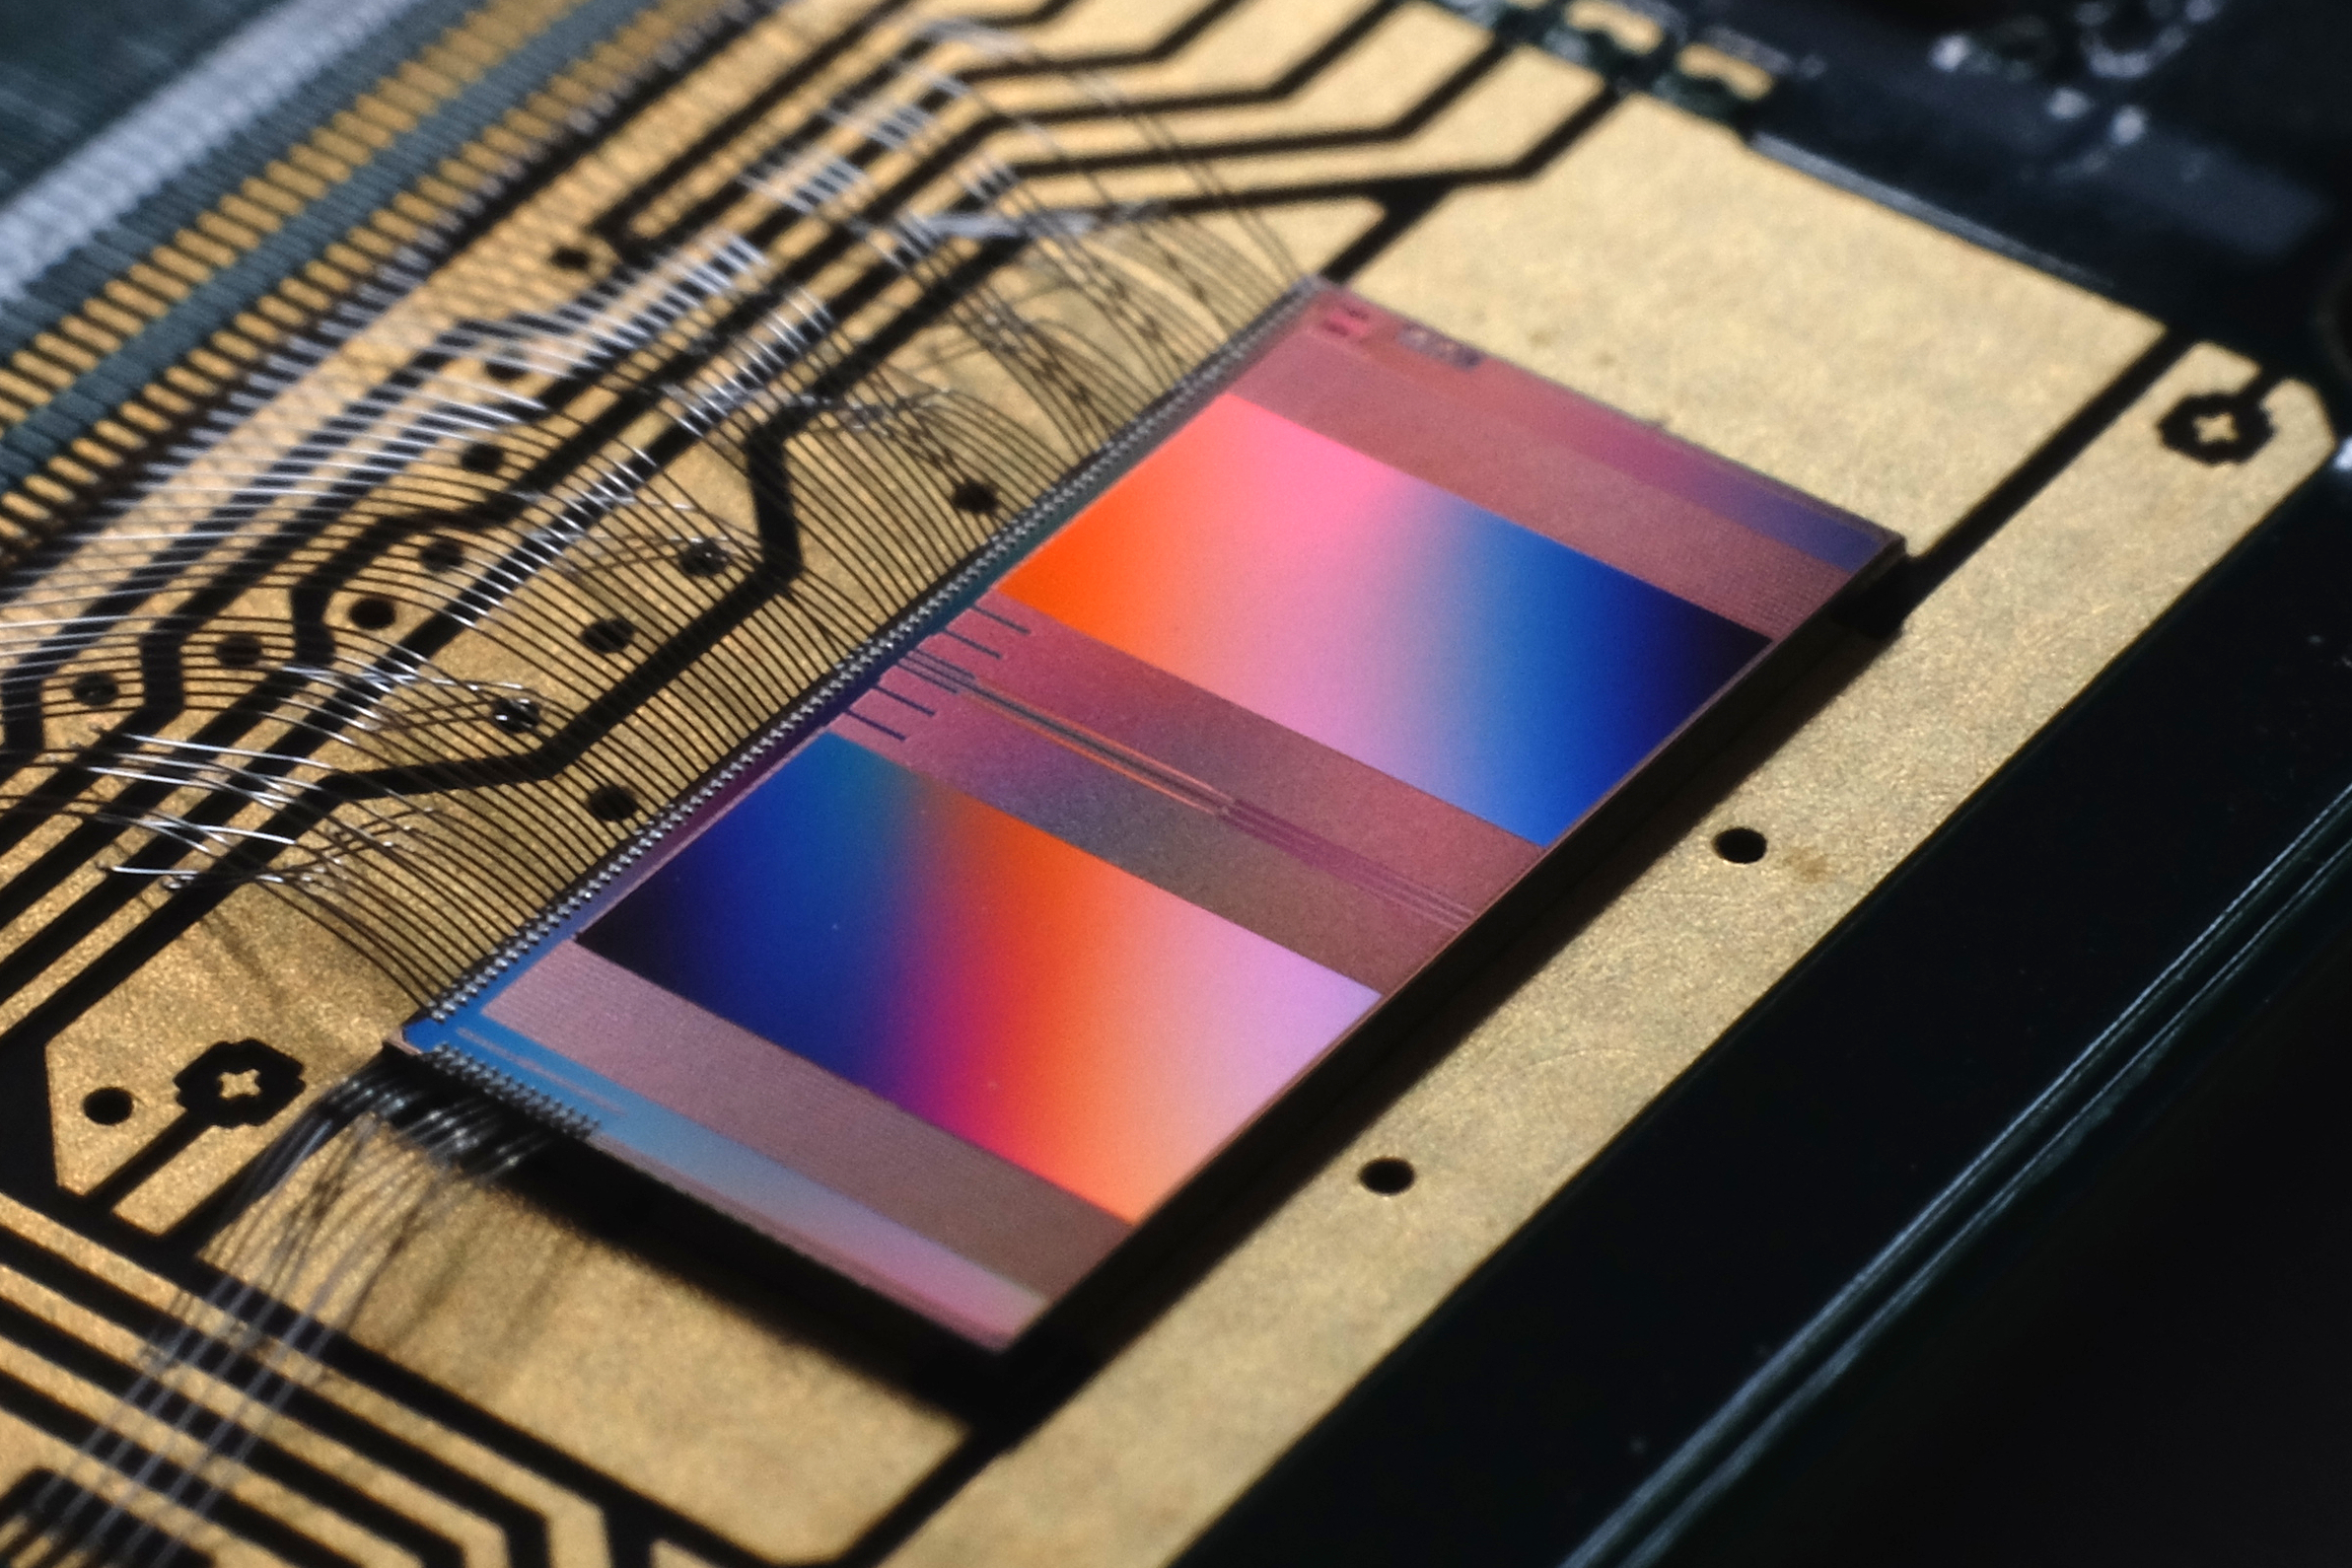
\includegraphics[width=0.4\textwidth]{figures/HXcloseup.JPG}
	\caption[Close-up of the newest \gls{bss2} single chip.]{Close-up of the newest \gls{bss2} single chip. The analog core of the neuromorphic chip is bonded before a protective cover is placed over it. Picture taken by M{\"u}ller, 2020.} 
	\label{hxcloseup}
\end{wrapfigure}

Certain tasks, such as pattern recognition, are quite difficult to solve with traditional computing methods.  Biologically inspired computing has provided a range of efficient approaches to successfully tackle these problems. In the same way, biology has also been the key inspiration for a new \emph{neuromorphic} hardware design. As it's paradigm, neuromorphic hardware is designed to be robust to malfunctioning sectors, energy efficient and adaptive. 

The experimental implementation of the presented learning strategies in \cref{neuralcoding} is done on \glsfirst{bss2}, a mixed-signal accelerated emulation platform for spiking neural networks which is funded by the EU's Human Brain Project (HBP) and is based in Heidelberg.

The \gls{bss2} platform is based upon a complete redesign of the \gls{hicann} chip from its predecessor \acrshort{bss1}. By using a smaller manufacturing process (\SI{65}{\nano \m} instead of \SI{180}{\nano \m}) several new features could be included on the new core - the \gls{hx}. The analog mixed-signal neuromorphic chip with 512 \gls{adex} neuron circuits and 256 possible synaptic connections per neuron is especially designed to investigate various on-chip plasticity algorithms. Therefore it features two \glspl{ppu}, on-chip event routing and the HAGEN extension. The latter is an early realization of a neuromorphic system which basically implements analog matrix multiplication on-chip (\citealp{schemmel2020accelerated}).

The new features have been tested step by step on smaller prototype systems, e.g. on the \gls{dls} the newly designed \gls{lif} neuron was tested. To avoid unnecessary costs, the size was reduced to $32$ neurons and a corresponding $32 \times 32$ synapse array allows all to all connectivity. Besides the Hagen extension and the \gls{adex} neuron, the main features of the \gls{bss2} platform, such as the \gls{ppu}, are already available on the prototyped versions.

%The experiments conducted within this thesis are done either on the \gls{hx} or the \gls{dls}. In the following section the individual parts of the chip are discussed.
%The manufacturing has been outsourced to the Taiwan Semiconductor Manufacturing Company (TSMC) using a standardized $65 \si{nm}$ low-power and low-leakage CMOS technology.

%refs: ibm http://www.research.ibm.com/articles/brain-chip.shtml
% coral board:
% Loihi:

\subsection{Architecture of \gls{bss2}}
\begin{figure}
	\begin{subfigure}[c]{0.5\textwidth}
		\centering
		\caption{}
		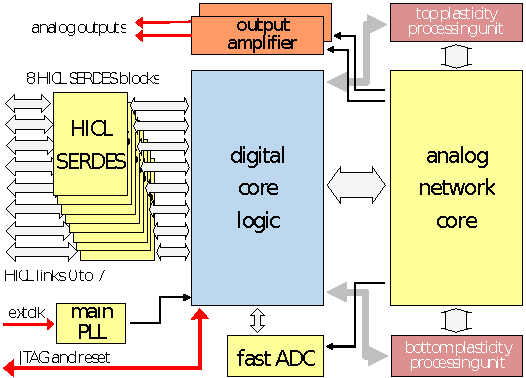
\includegraphics[width=0.9\textwidth]{figures/bss2architecture_wtext.pdf}
		\label{hxstructure}
	\end{subfigure}	
	\begin{subfigure}[c]{0.5\textwidth}
		\centering
		\caption{}
		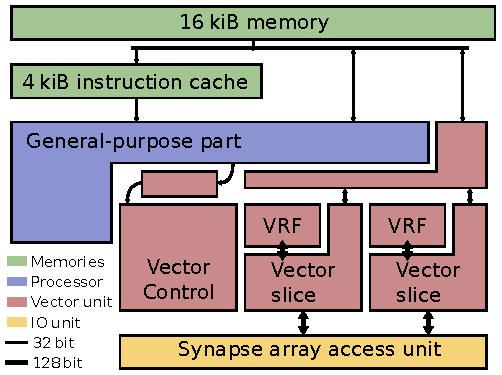
\includegraphics[width=0.9\textwidth]{figures/ppu_overview.pdf}
		\label{hxppu}
	\end{subfigure}
	\caption[Overview of the architecture on \gls{bss2}]{Overview of the architecture on \gls{bss2}. (\subref{hxstructure}): The neurmorphic platform is divided into a digital and analog core which is connected to an external host via an FPGA. Two plasticity processing units provide computational power for on-chip training.  Figure taken from \citealp{schemmel2017internal} (\subref{hxppu}): The plasticity processing units are divided into a general purpose part which is based on a 32-bit architecture and a vector unit, that enables efficient parallel data processing of analog parameters and observables. Figure taken from \citealp{friedmann2016hybridlearning}}
\end{figure}

The design of the \gls{hx} chip can be divided into an \emph{analogue} and \emph{digital} core (c.f. figure \ref{hxstructure}). The external communication is established by an \gls{fpga} accessing eight serial Low Voltage Differential Signaling (LVDS) link. The interface handles read/write instructions and manages spike event data in both directions.

The analogue core contains the physical implementation of the \gls{lif} and the \gls{adex} neuron model respectively (c.f. \citealp{aamir2018dls2neuron} and \citealp{aamir2018mixed}). The biological time constants of neurons and synapses are usually in the order of 1 to 100 milliseconds. The \textit{in-silico} implementation of the neuron models create a temporal speed-up compared to their \textit{in-vivo} counterpart, leading to chip time constants of a few microseconds. This acceleration is possible due to the supra-threshold dynamics of CMOS transistors. 

The analog neuron model parameters in both chips are tunable by setting bias currents over an 10-bit \gls{dac}, which allows to control and adjust each neuron individually (\citealp{hock13analogmemory}). The 10-bit spike counter of the \gls{dls} (one per neuron) has been replaced by a 8-bit counter in the \gls{hx}. 

\begin{figure}
	\centering
	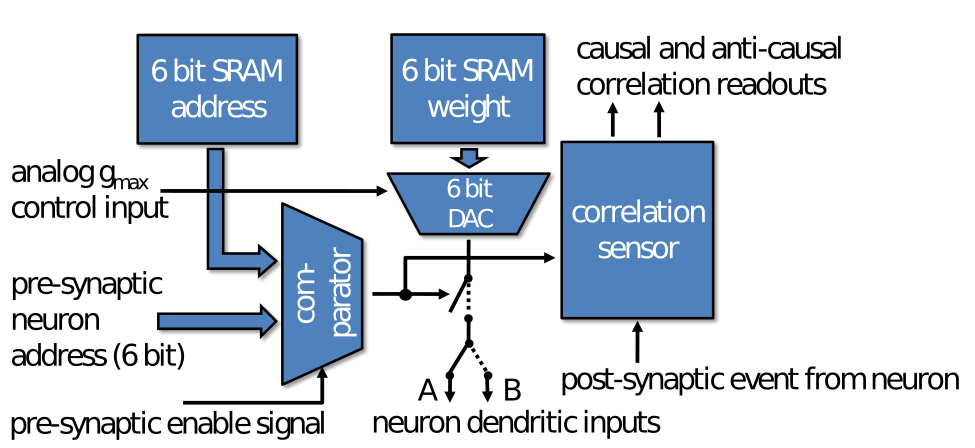
\includegraphics[width=0.8\textwidth]{figures/synapse.png}
	\caption[Synapse circuit overview on \gls{dls}]{Synapse circuit overview on \gls{dls}. Synapse drivers inject the presynaptic activity row-wise as either inhibitory or excitatory spikes. The 6-bit addresses of the presynaptic neuron is compared at each synapse with a local 6-bit address. If the addresses match, the spike is relayed to the corresponding neuron at the bottom of the synapse grid. The synaptic strength can be configured by a 6-bit weight. The two correlation sensors (causal and anti-causal) record \gls{stdp} traces. Figure from \citealp{friedmann2016hybridlearning}.}
	\label{synapseschematics}
\end{figure}

The neurons can be connected by a grid of $512 \times 256$ synapses ($32 \times 32$ on the prototypes). The activity of presynaptic neurons is injected row-wise by dedicated synapse drivers as either excitatory or inhibitory spikes. Each synapse has access to a 6-bit decoder address and compares it to a 6-bit label of the incoming spikes (see \cref{synapseschematics}). If they match, the spike is relayed to the corresponding neuron at the bottom of the synapse grid. The efficacy is thereby configured by a 6-bit weight.


In addition, two correlation sensors per synapse (causal and anti-causal) record \gls{stdp} traces and store them in dedicated capacitors. These analog observables can then row-wise readout by the \gls{ppu} using a \gls{cadc} with a total of 1024 \gls{cadc} channels (one channel per correlation sensor per synapse). Unlike for previous prototypes, the \gls{hx} has access to further observables such as the membrane potential and opens up new possibilities for implementation of plasticity rules. 

As an additional debugging and observation tool, a \gls{madc} can be accessed from the digital core to readout any available analog observables. However, the \gls{madc} readout is limited to a single observable making it not suitable for efficiently parallelized computing.

When training a highly accelerated analog system, such as \gls{bss2}, a fast computation of any plasticity rule is indispensable. To provide sufficient computational power, the chip is equipped with two \glspl{ppu}, each containing a general-purpose unit that is extended with a special function unit implementing \gls{simd} operations. The special function unit has vector-wise access to the synapse array as well as to the results of the \gls{cadc} and will be further referred to as \emph{vector unit}.

Apart from the dedicated spike counters, the digital neuron back end registers any spiking event and transfers them to the digital core logic, where the events are merged with any activity coming from the noise spike generators or \glspl{ppu} as well as from an external source. The events are then rerouted back into the synapse grid accordingly, enabling recurrent connections and multilayer network structures.

%The communication with an external host is streamed out to the controlling Field Programmable Gate Array (FPGA). The existing FPGA solution developed for \gls{bss1} was simply transfered to \gls{bss2}.
%The link between chip and external host is established via an \gls{fpga} accessing eight serial Low Voltage Differential Signaling (LVDS) links. This interface handles read/write instructions and manages spike event data in both directions. %The FPGA grants access for the PPU to greater memory storages than the one provided on-chip. Access to large training datasets is vital for most learning tasks.